%%
%% edengths.tex - LaTeX2e thesis driver
%%
%% Copyright (C) 1998 George Taylor
%% Copyright (C) 2010-2021 Mathew Topper <damm_horse@yahoo.co.uk>
%%
%% This file is part of the University of Edinburgh, Department of
%% Engineering LaTeX2e thesis template.
%% 
%%
%%   ABOUT
%%
%% This is the driver file for a Latex2e template which corresponds to the
%% regulations regarding layout of a thesis submitted within the University
%% of Edinburgh.

%%%% LOAD DOCUMENT CLASS

\documentclass[12pt,crest,nopardent,msfonts,fancychap,hyper,nomencl]{edengths}

%% Class options go in the square brackets above
%% i.e. \documentclass[options]{edengths}

%% Default report class options are:
%% (These are automatically included)
%%
%% a4paper
%% openright - Start chapters on righthand side pages
%% titlepage - Title should be on it's own page
%%


%% Standard available report class options are:
%%
%% 10pt
%% 11pt
%% 12pt
%% draft
%% final
%% fleqno
%% leqno
%% oneside
%% twoside

%% edengths class specific options:
%%
%% subsubnos - Enable numbering of subsubsections (note: these don't
%%             appear in the contents)
%% nosans    - Don't use sans serif fonts
%% nopardent - Remove paragraph indent and add a line skip
%% msfonts   - Use MS fonts rather than latex default
%% fancychap - Use fancy chapter headings like jthesis
%% crest     - Use a crest on the front page
%% labels    - Print labels in spine margin.
%% hyper     - Use the hyperref package to put clickable links into 
%%             the document. Use \autoref{fig:example} now instead of,
%%             say, figure~\ref{fig:example}. Settings are in
%%             edengfmt.tex.
%% nomencl   - Use the nomencl package. Example of it's usage are in
%%             front/nomencl.tex. The Nomenclature is called from
%%             front/frontmatr.tex

%% ADDITIONAL FORMATTING can be done in 'edengfmt.tex' where the page
%% dimensions, header/footers, table of contents and the names of 
%% the bibliography and other formatting settings can be altered.
%% IN PARTICULAR THE LINE SPACING IS SET IN 'edengfmt.tex' AND
%% THE HYPERREF OPTIONS ARE SET HERE TOO. THIS SETS THE NAME OF
%% THE PDF, FOR EXAMPLE.

%% The class file should automatically detect pdflatex and provide
%% the right options.

%%%% LOAD USER DEFINED PACKAGES.

%% These are in ``packages.tex'' file and is automatically loaded
%% by the class file

%%%% LOAD USER DEFINED COMMANDS.

%%
%% defintns.tex - User defined commands for edengths.tex
%%
%% Copyright (C) 2010-2017 Mathew Topper <damm_horse@yahoo.co.uk>
%%
%%
%%   ABOUT
%%
%% This file contains the user defined commands for a Latex2e template which
%% corresponds to the regulations regarding layout of a thesis submitted within
%% the University of Edinburgh.

%%%%%%%%%%%%%%%%%%%%%%%%%%%%%%%%%%%%%%%%%%%%%%%%%%%%%%%%%%%%%%%%%%%%%%%%%%
%%%%%%%%%%             Define your commands here              %%%%%%%%%%%%
%%%%%%%%%%%%%%%%%%%%%%%%%%%%%%%%%%%%%%%%%%%%%%%%%%%%%%%%%%%%%%%%%%%%%%%%%%

%% New commands can be written using
%%    \newcommand{command}[inputs]{definition}.
%% In the definition the inputs are accessed with #1, #2, etc.
%%
%% If you want to override an existing command use \renewcommand instead
%% of \newcommand. \newcommand with give an error if command is already
%% defined.

%% If you are concerned that your command might override a default
%% you can use \providecommand which will ignore the new command if
%% a command of that name already exists.

%%%%% Some Example Maths Definitions (only use in maths mode)

\newcommand{\pdif}[2]{\frac{\partial #1}{\partial #2}}
%% ie \pdif{x}{t} would give partial x over t.

\newcommand{\dpdif}[2]{\dfrac{\partial #1}{\partial #2}}
%% inline partial derivative ie for $\dpdif{x}{t}$.
%% (\dfrac needs amsmath package)

\newcommand{\Ddif}[2]{\frac{D #1}{D #2}}
%% Material derivative

\newcommand{\spdif}[2]{\frac{\partial^{2} #1}{\partial #2^{2}}}
%% second partial derivative.

\newcommand{\altspdif}[3]{\frac{\partial^{2} #1}{\partial #2 \partial #3}} 
% mixed second partial i.e. \altspdif{x}{z}{t} = d2x / dzdt

\newcommand{\ndif}[2]{\frac{\mathrm{d} \, #1}{\mathrm{d} #2}}
%% ordinary differential.

\newcommand{\sndif}[2]{\frac{\mathrm{d} \,^{2} #1}{\mathrm{d} #2^{2}}}
%% ordinary second differential.


%%%% SET THE PATH FOR DIAGRAMS.

\graphicspath{{chapter1/}{chapter2/}{chapter3}{chapter4/}}
% {chapter_5/}{chapter_6/}{appendix/}}

%%%% PATH TO CREST

%% If you're not using the default crest files add the path here.
%% The default files are found in the 'front' directory.
%% Note: latex needs a eps file, while pdflatex needs pdf or jpg.
% \crestfile{/path/to/crest.pdps}

%%%% TITLE DETAILS

%% Author
\author{Chuanli Huang}

%% Title
\title{Spatial Organisation and Dynamics of Centromeric Protein CENP-A and Shugoshin}

%% Qualification (Defaults to \textit{Doctor of Philosphy})
% \qualification{}

%% University (Defaults to \textsc{The University of Edinburgh})
% \university{}

%% Year of submission
\date{2023}

%% NOTE - IF YOUR USING hyper THEN THE ABOVE DETAILS NEED SET IN
%% edengfmt.tex AS WELL.

%%%% CHAPTERS TO INCLUDE

%% You may restrict which chapters are compiled using \includeonly
%% appendix/edengapp must be in the list if appendicies are included.

% \includeonly{front/frontmtr, chapter1/chapter1}
% \includeonly{chapter2/chapter2, chapter3/chapter3}
% \includeonly{chapter6/chapter6, appendix/edengapp,
%              appendix/appendx1 appendix/appendix2}

%%%% START DOCUMENT

\begin{document}
% \setcounter{tocdepth}{3}
%%%% FRONT MATTER

%%
%% frontmtr.tex - LaTeX2e thesis class
%%
%% Copyright (C) 2010-2017 Mathew Topper <damm_horse@yahoo.co.uk>
%%
%%
%%   ABOUT
%%
%% This is the frontmatter file for a Latex2e template which corresponds to the
%% regulations regarding layout of a thesis submitted within the University
%% of Edinburgh.
%%
%% The special formatting in the class requires the use of a particular command 
%% to call the front matter for everything before the table of contents. 
%% Just supply the path to the file containing the pre content front matter.
%% 

\makeprecontent{front/precntnt.tex}

%%%% TABLES AND LISTS

%% Table of contents
\tableofcontents

%% List of figure
% \listoffigures

%% List of tables
% \listoftables

%% List of figures and tables
\listoffiguresandtables

%% Make the nomenclature. This command won't do anything if nomencl option
%% is not declared.
\printnomenclature

%% Custom front matter chapters can be added using \input{frontchapter.tex}
%% For the correct title behaviour use the \frontchapter{title} command instead
%% of \chapter{title} at the start.


%%%% START MAIN BODY TEXT

%% Call the edengths wrapper.
\startbody

%% The template will work with part definitions (starred or otherwise), but note
%% that nameref and autoref may not work properly for referencing them.
% \part{The Fellowship of the Thing}

% \chapter{Introduction}
\section{Centromere is the specialised locus for chromosome segregation}

 The growth, healing and reproduction of all living organisms rely on cell division. Delivering an intact genome to the daughter cell challenges every dividing cell. Eukaryotes package their genomes into chromosomes, which must be replicated and segregated equally during each cell division. Severe diseases, such as cancer, genetic disorder and miscarriage, could arise if chromosome segregation is compromised \citep{Jallepalli2001ChromosomeMystery, Draviam2004ChromosomeStability, Wasielak-Politowska2022ChromosomeAging, Losada2014CohesinBeyond}. 
 
 Centromere is the specialised locus for chromosome segregation, where the chromosome is physically attached to the spindle \citep{Westhorpe2015AMaintenance, McKinley2015TheFunction, Talbert2020WhatCentromere, Fukagawa2014}. First described by \cite{Flemming1882ZellsubstanzZelltheilung} as primary constriction, it is visualised as the intersection point of the iconic X-shaped mitotic chromosome under a microscope. Lack of centromere, or being acentric, leads to chromosome loss during cell division. Although the appreciation of centromere function has been established since its discovery, the molecular feature underneath remained elusive due to the species-to-species variations and the complexity of players involved. \cite{Darlington1936TheEnquiry} therefore recommended defining the centromere in terms of the function rather than the form. Nevertheless, advances in molecular biology shed light on the form of centromere. In most species, the centromeric DNA sequence plays an important but not definitive role in centromere specification \citep{Hoffmann2020, Harrington1997FormationMicrochromosomes, Catania2015SequenceChromatin, Iwata-Otsubo2017, Kasinathan2018Non-B-FormCentromeres, Shukla2018CentromereCycle, Logsdon2019, Murillo-Pineda2020}. It is instead determined epigenetically by the histone H3 variant CENP-A \citep{Warburton1997ImmunolocalizationCentromeres, Vafa1997ChromatinPlate, Earnshaw1985ThreeChromosome, Liu2006MappingCells, Regnier2005CENP-ABubR1, Heun2006, Mendiburo2011, Barnhart2011, Logsdon2015}. The macromolecular protein complex consisting of around 100 subunits, kinetochore, is formed on the centromere to mediate the physical connection between the chromosome and spindle microtubules and act as a signalling hub to monitor the interaction \citep{Musacchio2017AFunction, McAinsh2022TheKinetochores, Cheeseman2014TheKinetochore, Hara2018KinetochoreExit}. Apart from the progress in the form of centromere, the strategies centromere adopts to execute its function have also been elucidated over the years \citep{Tanaka2013, Zhou2020EmergentChromosomes}. In the following sections, the form and function of the centromere will be described in more detail. 

\section{The form of centromere}
\subsection{The genetics}

The structure of centromeric DNA and its functional importance varies dramatically between species. Based on the chromosomal distribution, centromeres are classified as monocentromere, where the centromere is localised at a restricted region of the chromosome, and holocentromere, where the centromere spreads the entire length of the chromosome. Depending on size, the monocentromere can be further divided into point centromere, which contains a short DNA sequence of just over 100 bp, and regional centromere, which could be up to megabases long. The importance of underlying DNA sequences to centromere function could also be very different, ranging from pure genetic to mainly epigenetic. 

Point centromere, with a notable example budding yeast \textit{Saccharomyces cerevisiae}, is the simplest form and the first investigated at the molecular level. A budding yeast centromere consists of three elements \citep{Carbon1984StructuralCEN3}: CDEI, an 8-bp sequence that binds Cfb1 for H3 nucleosome eviction \citep{Niedenthal1993Cpf1I, Henikoff2011EpigenomeResolution}; CDEII, an AT-rich, around 80-bp sequence accommodating a single centromeric nucleosome containing Cse4, the budding yeast CENP-A, for kinetochore assembly \citep{Furuyama2007CentromereYeast, Henikoff2014TheVivo, Krassovsky2012TripartiteYeast} and CDEIII, a 25-bp sequence bound by the CBF3 complex \citep{Yan2018ArchitectureKinetochore}, which recruits the Cse4 chaperon Scm3, the budding yeast HJURP, for Cse4-containing nucleosome deposition \citep{Stoler2007Scm3Localization, Camahort2007Scm3Kinetochore}. Centromere specification is strictly genetic in this organism \citep{Clarke1980IsolationChromosomes, J1986SingleCerevisiae, Kingsbury1991Centromere-dependentVitro}, which could be explained by its unique centromere biology that factors for Cse4 nucleosome deposition are recruited by specific DNA sequences. This is in line with the observation that the exact sequences of CDEI and CDEIII are conserved across all 16 centromeres of budding yeast \citep{Clarke1998Centromeres:Eukaryotes, Baker2005GeneticCerevisiae}. As for the centromeric nucleosome accommodating sequence CDEII, only the length and AT abundance are conserved, supporting the notion from regional centromeres that CENP-A nucleosome binding does not require specific DNA sequences \citep{Bensasson2011EvidenceCentromeres}. The phylogeny indicated that point centromere species evolved from regional centromere species and this transition coincided with the emergence of 2-micron plasmid, a multicopy circular DNA capable of self-propagating in budding yeast \citep{Malik2009MajorComplexity}. Intriguingly, the 2-micron plasmid also uses a single locus called \textit{STB} to assemble a partitioning complex, which includes components of segregation machinery for normal chromosomes such as Cse4 and cohesin, for its association with the spindle microtubule \citep{Rizvi2018TheCerevisiae, Huang2011Evolution, Ghosh2007FaithfulSisters}. The outstanding resemblance led to the hypothesis that the point centromere is the domestication of the self-propagating locus of parasitic plasmids \citep{Malik2009MajorComplexity}. 

The regional centromere is the most common type of centromere. A typical regional centromere is AT-rich and possesses a modular structure composed of a CENP-A-nucleosome-accommodating central core flanked by heterochromatic domains called peri-centromere. The central core usually contains satellite DNA, short sequences repeated a large number of times, whereas the peri-centromere has less patterned sequences \citep{Talbert2020WhatCentromere, McKinley2015TheFunction, Wong2020LessonsChromosomes, Muller2019TheArchitecture}. As one of the fastest-evolving loci across the genome, the precise sequence of the centromere is extremely diverse among species \citep{Melters2013ComparativeEvolution}. Notably, due to the incompatibility of second-generation sequencing and repetitive sequence, deciphering the centromeric DNA sequence has been challenging. In fission yeast \textit{Schizosaccharomyces pombe}, the central core consists of non-repetitive \textit{cc} and inverted repeats \textit{imr} while the peri-centromere possess less ordered \textit{otr} composed of \textit{dg} and \textit{dh} repeats \citep{Chikashige1989CompositeSites, Clarke1993StructureCentromeres, Murakami1991StructureRegion, Nakaseko1986ChromosomeYeast, Nakaseko1987AChromosomes., Steiner1993CentromeresLoci}. Fruit fly \textit{Drosophila melanogaster} has a central core made up of a retroelement-enriched island flanked with AATAT and AAGAG satellites, and peri-centromeric chromatin containing mixed different types of short satellites that are neither conserved among chromosomes nor specific to the centromere \citep{Talbert2018SimpleSpecies, Wong2020LessonsChromosomes, Chang2019IslandsCentromeres}. House mouse \textit{Mus musculus} centromeres are close to telomeres, which is termed acrocentric. The central core and the peri-centromere consist of 120-bp minor satellites and 234-bp major satellites, respectively \citep{Komissarov2011TandemlyGenome, Kuznetsova2006High-resolutionDNA}. Primate including human \textit{Homo sapiens} central core contains 171-bp monomers, named $\alpha$-satellite, arranged into HOR arrays of different lengths, whereas the flanking peri-centromere is built with less structured monomeric $\alpha$-satellites that are less recognisable \citep{Maio1971DNAAethiops, Rosenberg1978HighlySIMIANSIMIANSIMIANSIMIANSIMIAN, Manuelidis1978ComplexDNAs, Manuelidis1978ChromosomalDNAs, Aldrup-MacDonald2014TheGenomics, Logsdon2021The8}. Unlike the point centromere, the centromeric DNA sequence is neither sufficient nor necessary for the function of the regional centromere \citep{McKinley2015TheFunction}. The former was indicated by the observations that the dicentric chromosomes due to the fusion of two normal chromosomes only assembled centromeric proteins, such as CENP-A, at one of the two endogenous centromeres \citep{Earnshaw1985ThreeChromosome, Steiner1994AYeast, Higgins2005EngineeredPlasticity, Sato2012EpigeneticChromosomes, Sullivan1995IdentificationCentromeres, Lange2009IsodicentricPalindromes}. The latter was evidenced by the fact the ectopic centromere, neocentromere, can form on chromosomal regions whose sequences bear little similarity with the canonical centromeres \citep{Marshall2008Neocentromeres:Evolution, Voullaire1993ACentromere, Tyler-Smith1999TransmissionGenerations, Amor2004HumanProgress}. The epigenetic notion was later confirmed by the elucidation of the requirement of CENP-A for centromere function and localisation \citep{Warburton1997ImmunolocalizationCentromeres, Vafa1997ChromatinPlate, Liu2006MappingCells, Regnier2005CENP-ABubR1, Heun2006, Mendiburo2011, Barnhart2011, Logsdon2015, Logsdon2019}. However, experimental results that cloned regional centromeric sequences were sufficient to support the inheritance of exogenous DNA suggest a contribution of sequence to \textit{de novo} centromere formation \citep{Hahnenberger1989ConstructionPombe., Haaf1992IntegrationSegregation, Harrington1997FormationMicrochromosomes, Ikeno1998ConstructionChromosomes}. This could partially be explained by the presence of the sequence-specific DNA-binding centromeric protein CENP-B \citep{Masumoto1989ASatellite., Muro1992CentromereBox., Earnshaw1985IdentificationScleroderma}. CENP-B is not essential for the centromere function as evidenced by that CENP-B knockout mice are still viable \citep{Kapoor1998TheMice, Perez-Castro1998CentromericAbnormalities, Hudson1998CentromereWeights}. But the centromere of the Y chromosome, which lacks CENP-B binding sequences called CENP-B box, failed to generate HACs \textit{in vivo} \citep{Harrington1997FormationMicrochromosomes, Grimes2002-SatelliteFormation}, consistent with the idea that centromeric DNA sequences facilitate the establishment of a functional centromere. The molecular mechanism was later uncovered that CENP-B interacts with both CENP-A and the CCAN component CENP-C to facilitate CENP-A deposition and kinetochore assembly \citep{Chardon2022CENP-B-mediatedCentromeres, Fachinetti2013, Fachinetti2015, Fujita2015StableNucleosome}. As mentioned above, the repetitiveness of centromeric sequences is a conserved feature in various regional centromere species and therefore evolutionarily preferred. Moreover, newly positioned centromeres from speciation, the ENCs, tend to gradually acquire repetitive sequences over time \citep{Rocchi2011CentromereMammals, Kasai2003ChromosomeEvolution}. The hypothesised mode of action is that younger sequences were inserted at the central core, pushing the old sequences towards the flank \citep{Locke2011ComparativeGenomes, Piras2010UncouplingEquus, Ventura2001CentromereEvolution, Kalitsis2012TheCentromere}, which was supported by the recently revealed complete human centromere sequences \citep{Logsdon2021The8}. The evolutionary preference for repetitive sequences also implied its importance to centromere function. It is speculated that tandem repeats might prevent the CENP-A domains from sliding along the centromere over cell cycles \citep{Nergadze2018BirthDomains}. 

Holocentromere refers to the situation where a diffused centromere extends along the whole length of the chromosome instead of a localised one \citep{Guerra2010NeocentricsRules}. It is often seen in flowering plants, insects, arachnids, and nematodes, including the model organism roundworm \textit{Caenorhabditis elegans} \citep{Wong2020LessonsChromosomes}. In mitosis, the holocentromere resides at the poleward faces of the chromosome whereas there is less of a common feature for meiosis \citep{Maddox2004HoloerElegans, Buchwitz1999AElegans, Marques2016HolocentromereHolocentromeres}. At the DNA sequence level, satellites and retrotransposons are enriched in the genome of holocentromere species but they lack an outstanding pattern as in regional centromere species \citep{Kang2016DifferentialElimination, Heckmann2013TheOrganization, Marques2016RestructuringPubera}. In beak-sedge \textit{Rhynchospora pubera} and \textit{C. elegans}, CENP-A nucleosomes do indicate a preferred association with certain DNA sequences \citep{Marques2016HolocentromereHolocentromeres, Gassmann2012AnElegans, Steiner2014HolocentromeresHotspots}. But the fact that these sequences are also actively transcribed suggests the possibility that CENP-A nucleosomes are preferentially loaded at these sites due to their accessibility created by the transcription factors. Indeed, when assessing the importance of DNA sequences for centromere formation in \textit{C. elegans}, it was found that the inheritance of WACs and generation of functional holocentromeres were independent of the DNA sequences used \citep{Stinchcomb1985ExtrachromosomalElegans, Yuen2011RapidEmbryos}. Interestingly, holocentromere has emerged multiple times independently in evolution, termed as convergent evolution in Genetics \citep{Guerra2019MonocentricFamily, Drinnenberg2014RecurrentInsects, Melters2012HolocentricAnalysis}, suggesting a selective force favouring the phenotype. It is unclear what the driver is but one hypothesis is that holocentromere can prevent the loss of fragmented chromosomes due to ionising radiation \citep{Zedek2018HolocentricLand}. Besides the three types of centromere mentioned above, there exists another variety where a few large distinct centromeric domains co-exist on a chromosome, called meta-polycentromere, which is recognised as the intermediate of holocentromere evolution \citep{Neumann2012StretchingDomains}. 

\begin{figure}[htbp]
  \centering
  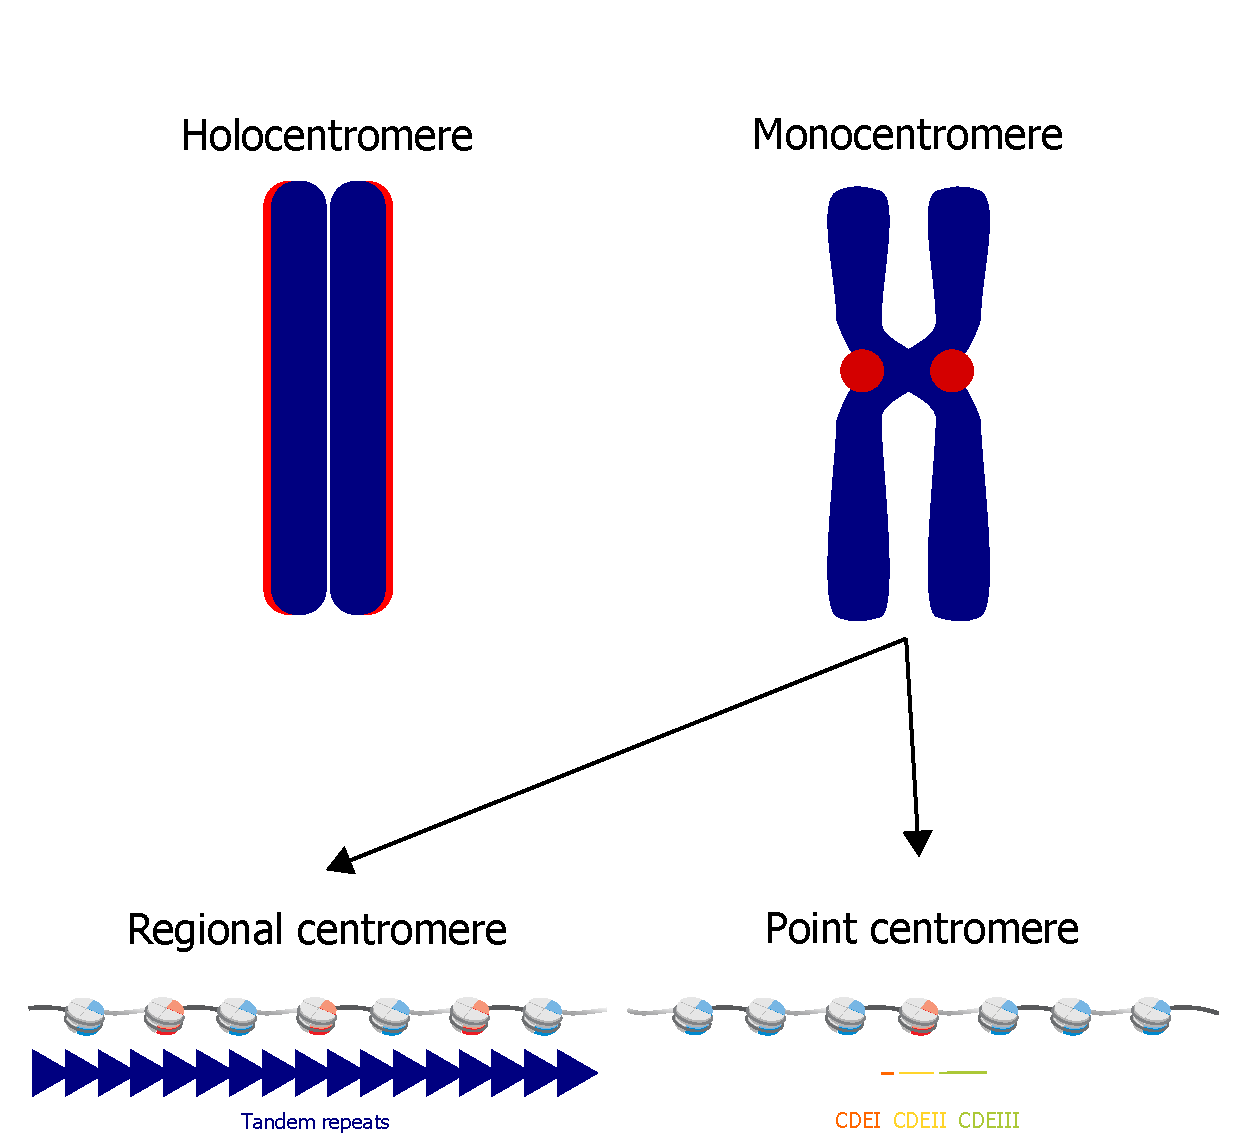
\includegraphics[width=0.9\textwidth]{chapter1/figures/centromere types.pdf}
  \caption[Different types of centroemres]{Different types of centroemres. Broadly, centromeres can be classified into holocentromere or monocentromere, depending on whether a diffused or localised centromere (red) is assembled on the chromosome (blue) under a microscope. Based on the length of DNA sequences and the number of CENP-A nucleosomes, monocentromere can be further divided into regional centromere or point centromere. A regional centromere usually possesses repetitive DNA sequences up to megabases in length and a large number of CENP-A nucleosomes. A point centromere is only composed of over 100 bp DNA sequences and one single CENP-A nucleosome. }
  \label{fig:cenTypes}
\end{figure}

Another common feature of centromeric DNA is the presence of non-B form DNA \citep{Kasinathan2018Non-B-FormCentromeres}, which refers to DNA structures other than the canonical one, such as hairpins and i-motifs. The former has been observed in humans, \textit{Drosophila melanogaster}, old-world monkeys and budding yeast while the latter has been seen in \textit{Drosophila dodeca} and humans \citep{Koch2000NeocentromeresDNA, Ferrer1995CentromericStructures, Catasti1994UnusualCentromeres}. <10-bp dyad symmetries found in many organisms are thought to be responsible for the formation of non-B form DNA. Notably, it is not the case for great apes and mice \citep{Kasinathan2018Non-B-FormCentromeres}. Nevertheless, non-B form DNA can still be detected by permanganate-seq in both species \citep{Kouzine2017Permanganate/S1Genome, Kouzine2013GlobalLymphocytes}. This was attributed to an alternative mechanism where their unique CENP-B boxes are bound by CENP-B, which is thought to induce DNA bending and the formation of non-B form DNA. In line with the idea, the human Y chromosome, which lacks CENP-B boxes, does possess short dyad symmetries \citep{Kasinathan2018Non-B-FormCentromeres}. The extent of effect and mechanism by which non-B form DNA contributes to centromere formation are not known. But it is speculated to facilitate HJURP localisation because the Holliday junction that HJURP binds \textit{in vitro} \citep{Kato2007ActivationCells} might represent short cruciforms enriched at centromeres \textit{in vivo} \citep{Kasinathan2018Non-B-FormCentromeres}. 

\nomenclature{CDE}{Centomere DNA Element}
\nomenclature{CBF}{Centromeric DNA Binding Factor}
\nomenclature{ENC}{Evolutionarily New Centromere}
\nomenclature{HOR}{Higher-Order Repeat}
\nomenclature{HAC}{Human Artificial Chromosome}
\nomenclature{WAC}{Worm Artificial Chromosome}
\nomenclature{i-motif}{intercalated motif}

\subsection{The epigenetics}

As mentioned above, early work with dicentric chromosomes and neocentromeres implied an epigenetic nature of the centromere. In most organisms, the DNA sequences are neither sufficient nor necessary for centromere function. The defining feature of a centromere is instead attributed to the presence of CENP-A-containing nucleosomes. Discovered as the antigen recognised by the 'anti-centromere' antibodies from patients of the autoimmune disease CREST syndrome, CENP-A is found to be enriched at the centromere \citep{Earnshaw1985IdentificationScleroderma}. Subsequent work identified CENP-A to be a variant of histone protein H3 \citep{Palmer1987AHistones, Palmer1990TheNuclei, Palmer1991PurificationHistone., Palmer1985KinetochoreMononucleosomes, Sullivan1994HumanCentromere., Buchwitz1999AElegans, Henikoff2014TheVivo, Takahashi2000RequirementYeast}. Extensive evidence pointed to the determining role of CENP-A in centromere specification. Apart from the canonical centromeres, it is always present at both the active centromeres of dicentric chromosomes \citep{Earnshaw1985ThreeChromosome} and neocentromeres \citep{Marshall2008Neocentromeres:Evolution}. The assembly of the kinetochore, the centromere effector, is strictly dependent on CENP-A \citep{Fachinetti2013, Liu2006MappingCells, Regnier2005CENP-ABubR1}. Moreover, artificial tethering of CENP-A to ectopic loci is sufficient to generate functional centromeres that mediate kinetochore-microtubule interactions and direct chromosome segregation \citep{Heun2006, Mendiburo2011, Barnhart2011, Logsdon2015, Logsdon2019, Roure2019}. 

The distinct biochemical characteristics of CENP-A form H3 have been suggested to account for its ability to confer centromere specification and kinetochore assembly. At the sequence level, CENP-A possesses an N-terminal tail not only largely different from H3 \citep{Sullivan1994HumanCentromere.} but also poorly conserved among species \citep{Goutte-Gattat2013PhosphorylationFunction} and a histone-fold domain that bears 62\% identity with H3. The first loop and second $\alpha$-helix of the histone-fold domain are collectively called CATD for their necessity in the centromeric localisation of CENP-A \citep{Black2007}. Consistently, the chimeric protein of H3 introduced with CATD is capable of being enriched at the centromere \citep{Black2007a}. The dependence of centromere targeting on CATD has been attributed to its interaction with the CENP-A chaperone HJURP \citep{Zhou2011StructuralScm3, Bassett2012, Hu2011StructureHJURP, Shuaib2010HJURPCentromeres}, which is responsible for the deposition of new CENP-A. This region has also been found to directly bind the CCAN component CENP-N \citep{Logsdon2015, Carroll2010, Carroll2009} and, together with the extreme C-terminus, mediate the interaction with the kinetochore assembly 'blueprint' CENP-C \citep{Carroll2010, Kato2013Spt6H3, Guse2011, Walstein2021}. At the structural level, CENP-A nucleosomes are more compact compared to H3 nucleosomes due to the physical properties of CATD \citep{Black2004, Sekulic2010}. The importance of this unique structure to centromere formation is implicated by the result that mutating residues within CATD that are responsible for the structural difference from H3 nucleosomes severely compromised the centromeric localisation of CENP-A \citep{Sekulic2010}. Furthermore, chromatin with CENP-A nucleosomes has a more condensed structure, likely via CENP-C and CENP-N \citep{Panchenko2011, Geiss2014, Zhou2022}. 

As with other epigenetics marks, CENP-A nucleosomes are challenged by cell cycle events and have to be properly propagated at the same locus over generations. This is important because errors in centromere propagation will be directly translated into inaccurate chromosome segregation, which leads to genome instability \citep{McClintock1939TheMeiosis, Koshland1987ACerevisiae}. The molecular mechanisms by which CENP-A is propagated are still under active research. The current knowledge of this topic will be introduced in Chapter 2 in detail. In brief, CENP-A nucleosomes are diluted in S phase because of DNA replication and replenished in anaphase or the next G1 of each cell cycle. The replenishment of new CENP-A nucleosomes depends on a positive feedback loop, consisting of CENP-C, HJURP, the MIS18 complex and deposited CENP-A, and a permissive chromatin environment. Mechanisms exist to ensure the resistance of CENP-A nucleosomes to chromatin remodelling events other than DNA replication, resulting in an extremely low turnover rate. The specificity of CENP-A to the centromere is mediated by 'sculpting' mechanisms, which selectly destabilise CENP-A nucleosomes outside centromeric chromatin. 

\nomenclature{CREST}{Calcinosis, Raynaud phenomenon, Esophageal dysmotility, Sclerodactyly and Telangiectasia}
\nomenclature{CATD}{CENP-A-Targeting Domain}

\subsection{The kinetochore}

Proteins carry out nearly all cellular functions. The same applies to the centromere, where the macromolecular protein assembly formed \textit{in situ} called kinetochore, which was originally an equivalent term to centromere \citep{Sharp1921IntroductionCytology, Darlington1936TheEnquiry} but later assigned to the protein complex, is responsible to execute its functions \citep{McAinsh2022TheKinetochores, McKinley2015TheFunction, Musacchio2017AFunction}. Moreover, the formation of a kinetochore in turn reshapes the spatial conformation of centromeric and peri-centromeric chromatin \citep{McAinsh2022TheKinetochores}. Thus, understanding the assemblage of the kinetochore is the key to building up the connection between the form and function of the centromere.

To achieve the highly-demanding, complicated functions of the centromere (to be introduced in Chapter 1 Section 1.3), the kinetochore has evolved an astonishing complexity. For example, in humans, multiple copies of about 100 different proteins are arranged into several self-organising subassemblies to constitute the kinetochore \citep{Cheeseman2014TheKinetochore}. \cite{McAinsh2022TheKinetochores} classified the kinetochore into four subassemblies (Figure~\ref{fig:KTSchematics}), ordered by their proximity to the underlying DNA, namely subassembly I, the CENP-A nucleosomes themselves and the DNA-binding CENP-B; subassembly II, the protein complex called CCAN that recognises CENP-A nucleosomes and stays at the centromere independent of the cell cycle stage, which can also be addressed as ICEN or the inner kinetochore; subassembly III, the critical interface that mediates the interaction with the microtubules called KMN-S network, which can also be termed as the outer kinetochore and subassembly IV, a fibrous corona-shaped structure facilitating the proper microtubule binding, which is consisted of RZZ-S complexes, motor proteins and SAC components. On top of this, another layer of complexity exists that the composition and stoichiometry of the kinetochore show abundant dynamics in response to the kinetochore-microtubule attachment status and the cell cycle stages. For instance, subassembly IV is only assembled on kinetochores unattached to microtubules and the presence window of subassembly III is from prophase to anaphase in animal cells \citep{Hara2020DynamicsProgression}. The components and regulations of each subassembly will be discussed in the following paragraphs with the exception of subassembly I, as they have been introduced in the previous sections. 

\begin{figure}[htbp]
  \centering
  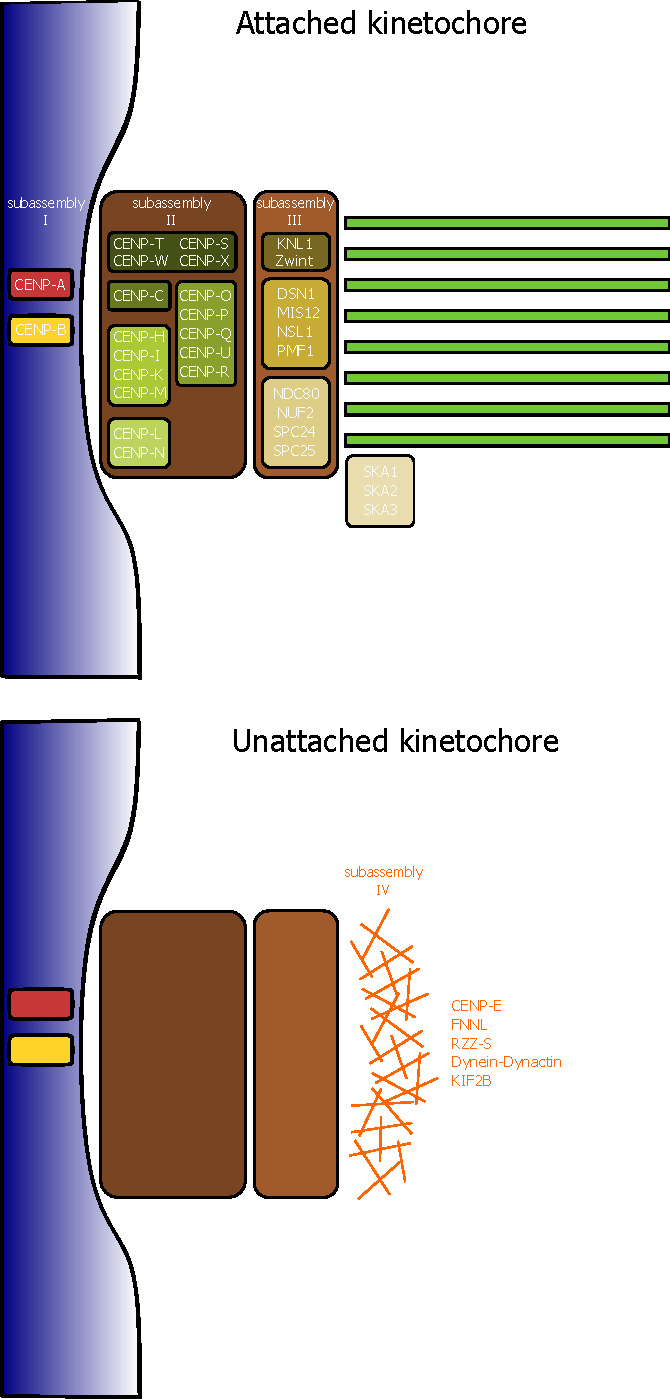
\includegraphics[width=0.9\textwidth]{chapter1/figures/kinetochore.pdf}
  \caption[Schematics of human kinetochore]{Schematics of human kinetochore. The human kinetochore is divided into four subassemblies as described by \cite{McAinsh2022TheKinetochores}. Moving away from centromeric chromatin, subassembly I contains CENP-A and CENP-B. Subassembly II, the inner kinetochore, consists of five subcomplexes, namely CENP-C, CENP-LN, CENP-HIKM, CENP-TWSX and CENP-OPQUR. Subassembly III, the outer kinetochore, is composed of KNL1, MIS12, NDC80 and SKA complexes. On unattached kinetochores, subassembly IV, the corona, forms, which comprises CENP-E, FNNL complex, RZZ-S complex, DD and KIF2B. }
  \label{fig:KTSchematics}
\end{figure}

In human cells, subassembly II, or the CCAN, is composed of 16 different proteins and can be further divided into five subcomplexes \citep{Foltz2006, Izuta2006ComprehensiveCells, Okada2006}. Central to its assembly is CENP-C \citep{Milks2009DissectionAssembly, Przewloka2011CENP-CAssembly}. Although classified in subassembly II, CENP-C is recognised as the 'blueprint' \citep{Walstein2021, Klare2015CENP-CKinetochores} of the whole kinetochore because it sequentially, from N- to C-terminus, contains a MIS12 complex (assembly III) binding site \citep{Screpanti2011DirectKinetochore, Gascoigne2011, Petrovic2016StructureKinetochores}, CCAN subcomplexes (assembly II) binding sites \citep{Klare2015CENP-CKinetochores, McKinley2015, Pentakota2017DecodingCENP-N, Nagpal2015} and CENP-A nucleosomes (assembly I) binding sites \citep{Carroll2010, Kato2013ACENP-C}. With the scope of CCAN, CENP-C interacts with CENP-HIKM and CENP-LN \citep{Klare2015CENP-CKinetochores, McKinley2015, Pentakota2017DecodingCENP-N, Nagpal2015}. Recent cryo-EM data on human CCAN bound to a CENP-A nucleosome revealed that, alongside the CENP-A nucleosome, the CCAN excluding CENP-C forms a gate-like structure wrapping the linker DNA, with CENP-C connecting the two structures. Within the gate-like structure, CENP-OPQUR and CENP-HIKM formed two pillars; CENP-LN formed the arc and CENP-TWSX formed the base \citep{Yatskevich2022StructureNucleosome, Pesenti2022StructureOrganization}. Despite the low level of sequence conservation, budding yeast CCAN, Ctf19 complex, indicated a highly similar structure to human CCAN by cryo-EM \citep{Yatskevich2022StructureNucleosome, Pesenti2022StructureOrganization, Hinshaw2019TheYeast, Yan2019StructureNucleosome}, suggesting a potential generality of eukaryotic kinetochore assembly principles and that the large kinetochores of higher eukaryotes might simply be multiple copies of budding yeast kinetochores \citep{Walstein2021, McAinsh2022TheKinetochores}. However, the importance of the CCAN is compromised by the non-essentiality of the components. In budding yeast, only 3 out of 14 components are required for cell viability \citep{DeWulf2003HierarchicalSubcomplexes, Fernius2009EstablishmentCsm3, Measday2002Ctf3pKinetochore, Ortiz1999AKinetochore, Pot2003Ch14pKinetochore}. In human cells, variable results existed due to the acuteness and completeness of protein depletion and the types of cells used \citep{Foltz2006, McKinley2015, Nguyen2021DifferentialPathways, Pesenti2018ReconstitutionNDC80, Raaijmakers2018BUB1Compromised}. The non-essentiality of the CCAN components and varied requirements of each component for different species might be due to the complexity of the network allowed a large degree of freedom and led to flexibility throughout evolution. 

Sometimes referred to as the KMN-S network, subassembly III is built from four subcomplexes, KNL1, MIS12, NDC80 and SKA complexes \citep{DeWulf2003HierarchicalSubcomplexes, Theis2009ComparativeDivision, Bharadwaj2004IdentificationComplex, McCleland2003TheActivity, Desai2003KNL-1Elegans, Obuse2004AZwint-1, Wigge2001TheSegregation, Westermann2003ArchitectureCore, Cheeseman2004ATension, Cheeseman2006TheKinetochore, Nekrasov2003InteractionsCerevisiae, Pinsky2003AnKinase, Kline2006, Welburn2009TheMotility, Gaitanos2009StableSka3/C13Orf3}. It is localised on subassembly II the inner kinetochore, facing the opposite direction of DNA, hence is also called the outer kinetochore, and directly mediates the interaction between the kinetochore and microtubules. The KNL1 complex is the signalling hub of the cell cycle checkpoint monitoring the status and correctness of kinetochore-microtubule attachment, which is termed SAC (to be introduced in Chapter 1.3.1). It is a heterodimer composed of KNL1 and ZWINT, with the structure and function of the former well studied whereas that of the latter largely remained unknown. From N- to C-terminus, the KNL1 protein possesses a PP1 binding motif that might be under the phospho-regulation by Aurora B \citep{Liu2010RegulatedKinase, Rosenberg2011KNL1/Spc105Checkpoint, Roy2019}, MELT motifs whose phosphorylation by MPS1 forms docking sites for the key SAC signalling proteins BUB1-BUB3 complex \citep{Cheeseman2004ATension, Primorac2013Bub3Signaling, Shepperd2012, Yamagishi2012MPS1/Mph1Components, Vleugel2013ArrayedSegregation, London2012}, which then recruits MAD1-MAD2 complex and BUB3-BUBR1-PP2A complex \citep{Suijkerbuijk2012IntegrationAttachments, Kruse2013DirectProgression, Krenn2012StructuralInteraction}, a ZWINT-binding motif predicted to form a coiled-coil structure \citep{Petrovic2010TheAssembly} and RWD domains interacting with the stalk of MIS12 and NSL1 \citep{Petrovic2014ModularOrganization}. The delicate interplay among kinases and phosphatases present on KNL1 is central to SAC signalling \citep{Saurin2018KinaseKinetochore}. The MIS12 complex forms the linkage connecting subassembly II and the other subcomplexes of subassembly III. Four structural paralogs, DSN1, MIS12, NSL1 and PMF1, compose the Y-shaped complex \citep{Petrovic2010TheAssembly, Petrovic2016StructureKinetochores, Dimitrova2016StructureAssembly, Hornung2011MolecularComplex, Maskell2010MolecularComplex}. The tips of the Y interact with the CCAN \citep{Screpanti2011DirectKinetochore} while the stalk binds both the KNL1 and NDC80 complexes \citep{Petrovic2014ModularOrganization}. The interaction between the MIS12 complex and CCAN relies on the direct binding of MIS12 protein to CENP-C, which requires the phosphorylation of DSN1 by Aurora B which exposes the binding site \citep{Kim2015, Akiyoshi2013TheYeast, Bonner2019EnrichmentAssembly, Hara2018MultipleKinetochores, Rago2015DistinctCENP-T, Zhou2017PhosphorylationMitosis}. This requirement has been proposed to prevent kinetochore assembly by non-centromeric CENP-C. The NDC80 complex, together with the SKA complex, is responsible for the capture of spindle microtubules \citep{Cheeseman2006TheKinetochore, Wimbish2020Hec1/Ndc80Interface, DeLuca2006KinetochoreHec1}. It consists of an NDC80-NUF2 and an SPC24-SPC25 heterodimer. The two dimers possess a very similar structure composed of a globular head and a coiled-coil stalk \citep{Wei2006StructureDomain, Wei2005MolecularComponent, Wei2006TheAttachment, Ciferri2005ArchitectureKinetochore, Ciferri2008ImplicationsComplex}, except that NDC80-NUF2 has a break in the stalk, which is believed to provide rotational freedom \citep{Tang2013Ndc80Motif}. The SPC24-SPC25 dimer binds both the MIS12 complex and the CCAN through the interaction between its RWD domains and MIS12 protein or CENP-T. On the opposing end, the CH domain of the NDC80-NUF2 dimer mediates the interaction with microtubules. The NDC80 complex undergoes jackknifing in the absence of microtubule binding \citep{Roscioli2020, Scarborough2019TightMicrotubules}. Evidence has been reported linking this conformational change to the attachment-sensing function of SAC \citep{Wan2009ProteinSite, Aravamudhan2015TheSignalling}. In metazoa, subassembly III of attached kinetochores further contains the SKA complex to enhance microtubule binding \citep{Welburn2009TheMotility, Gaitanos2009StableSka3/C13Orf3, Theis2009ComparativeDivision}. The SKA complex is a W-shaped complex dimerised from trimers comprising SKA1, SKA2 and SKA3, with the microtubule-binding domain of SKA1 located at the tip of the W \citep{Abad2014StructuralComplex, Jeyaprakash2012StructuralInterface, Schmidt2012TheProtofilaments}. The interaction between SKA3 and coiled coils of the NDC80 complex has been shown to facilitate microtubule binding \citep{Abad2016Ska3Domain, Chan2012AuroraInteraction, Helgeson2018HumanAttachments, Zhang2017Ska3Progression}. Although lacking direct orthologs, budding yeast has a functional equivalent to the SKA complex, named the Dam1 complex. It is a heterodecamer that is able to assemble a ring-like structure with other fifteen copies \citep{Jenni2018StructureInterface, Miranda2005TheMicrotubules, Ramey2011TheMicrotubule, Westermann2005FormationComplex}. Two Dam1 complex rings are present on each kinetochore \citep{Kim2017TheRings}. Similar to the SKA complex, the DAM1 complex associates with the kinetochore in the presence of microtubules \citep{Li2002TheKinetochore} and strengthens their interactions \citep{Lampert2013MolecularComplexes, Lampert2010TheComplex, Tien2010CooperationB}. 

First discovered by EM, subassembly IV, or the corona, is a diffuse fibrous structure specific to unattached kinetochores of metazoan cells \citep{Jokelainen1967TheCells}. It is highly dynamic and undergoes expansion or shrinkage depending on the attachment status of the kinetochore \citep{Kops2020CrowningSegregation}. Known proteins showing corona localisation include the RZZ complex, Spindly, DD, CENP-E, CENP-F, MAD1-MAD2 complex and Cyclin B \citep{McAinsh2022TheKinetochores}. The RZZ complex, composed of ROD, ZW10 and ZWILCH, is recognised as the core because its depletion but not the others led to a complete loss of the corona \citep{Rodriguez-Rodriguez2018DistinctExpansion, Kops2005ZW10Kinetochore, Silio2015KNL1-BubsKinetochores, Varma2013SpindleKinetochores, Auckland2020CENP-FCargoes, Currie2018Bub1Cells}. Spindly is recruited to dimerised RZZ complexes via the interaction with ROD \citep{Mosalaganti2017StructureSpindly, Pereira2018Self-AssemblyAttachment, Raisch2022StructureKinetochores}, which requires the farnesylation of Spindly that releases it from autoinhibition \citep{Sacristan2018DynamicMitosis}. The motor proteins DD are subsequently recruited to the complex by Spindly \citep{Mosalaganti2017StructureSpindly}. However, the mechanism by which the RZZ-S complex itself assembles on subassembly III is unknown. Some of the corona-localised proteins have RZZ-S-independent localisation mechanisms \citep{Ciossani2018TheKinases, Rodriguez-Rodriguez2018DistinctExpansion}. The kinesin CENP-E and CENP-F are distantly related paralogs and are recruited via the kinase domain (or the pseudokinase domain for BUBR1) of SAC components BUB1 and BUBR1, which are another pair of paralogs \citep{Ciossani2018TheKinases, Berto2018DisentanglingKinetochores}. Corona-localised MAD1-MAD2 complexes are recruited in a manner independent of the conventional BUB1-dependent pathway \citep{Pereira2018Self-AssemblyAttachment}, suggesting that they represent a distinct pool. Although still elusive, the corona-associated Cyclin B might be responsible for recruiting this pool \citep{Allan2020CyclinCheckpoint}. The expansion of the corona requires the RZZ-S complex whose ROD and ZWILCH are phosphorylated by MPS1 \citep{Rodriguez-Rodriguez2018DistinctExpansion, Sacristan2018DynamicMitosis, Pereira2018Self-AssemblyAttachment}, whereas the shrinkage depends on DD and Spindly \citep{Sacristan2018DynamicMitosis, Gassmann2010RemovalCells, Howell2001CytoplasmicInactivation}. The apparent negative feedback might exist to allow prompt disassembly once proper microtubule attachment is established. The corona is believed to ensure the speedy and accurate establishment of proper kinetochore-microtubule attachment \citep{Kops2020CrowningSegregation}. Through dynamical expansion and shrinkage, it could facilitate lateral capture of unattached kinetochores by astral microtubules, lateral to end-on attachment conversion, microtubule nucleation from the unattached kinetochore and SAC signalling. 

The kinetochore further affects the structural organisation of centromeric and peri-centromeric chromatin. Due to the fact that methods to study the chromatin localisation of proteins and chromosomal conformation rely heavily on sequencing-based technologies, evidence supporting the argument is mainly from the point centromere species budding yeast, whose centromeric and peri-centromeric DNA sequences are non-repetitive. The SMC complex cohesin is found to be enriched at the core centromere and the two peri-centromere borders \citep{Eckert2007TheTension, Fernius2009EstablishmentCsm3, Fernius2013Cohesin-DependentEstablishment, Glynn2004Genome-WideCerevisiae, Weber2004TheBinding}. It is targeted to the centromere by the direct interaction between the cohesin loader Scc2-Scc4 and the CCAN component Ctf19 phosphorylated by DDK \citep{Hinshaw2015StructuralLoading, Hinshaw2017TheComplex}. Later chromosomal conformation study confirmed that an intrachromosomal loop was formed on each side of the core centromere, physically connecting it to the peri-centromeric borders \citep{Paldi2020ConvergentPericentromeres}. This special conformation appeared to be functional as artificial enlarging of the centromeric loops of merely one chromosome was sufficient to increase chromosome segregation errors \citep{Paldi2020ConvergentPericentromeres}. Apart from this, the kinetochore-localised kinase Bub1 recruits the peri-centromeric protein shugoshin Sgo1 and it in turn recruits another SMC complex condensin to the peri-centromeric chromatin, which has been proposed to generate a back-to-back geometry of sister kinetochores that facilitates proper kinetochore-microtubule interactions \citep{Indjeian2007, Verzijlbergen2014}. 

\nomenclature{ICEN}{Interphase CENtromere complex}
\nomenclature{KMN-S}{Knl1, Mis12, Ndc80 and Ska}
\nomenclature{RZZ-S}{Rod-Zw10-Zwilch-Spindly}
\nomenclature{FNNL}{CenpF-Nde1-Ndel1-Lis1}
\nomenclature{EM}{Electron Microscopy}
\nomenclature{MELT}{methionine(M)-glutamic acid(E)-leucine(L)-threonine(T)}
\nomenclature{RWD}{RING finger-containing proteins, WD repeat-containing proteins, and DEAD (DEXD)-like helicases}
\nomenclature{CH}{Calponin Homology}
\nomenclature{DD}{Dynein-Dynactin}
\nomenclature{DDK}{Dbf4-Dependent Kinase}
\nomenclature{SMC}{Structural Maintenance of Chromosomes}

\section{The function of centromere}

The major function, if not the sole one, of the centromere is to segregate chromosomes faithfully. To accomplish this non-trivial task, it adopts a range of delicate strategies. \textbf{a)} chromosomes are attached to the spindle microtubules through the 'search and capture' principle, where microtubules dynamically grow and shrink to find kinetochores and establish attachment once encountered. Kinetochores promote the occurrence of the stochastic event via several mechanisms, such as localising themselves to limited space, changing geometric architecture according to the attachment status (Chapter 1 Section 1.2.3) and nucleating non-spindle microtubules in proximity to facilitate the growth of spindle microtubules. Detailed information on this field can be found in the review by \cite{Renda2021RoleMorphogenesis}. \textbf{b)} During mitosis, the kinetochores of sister chromatids have to be attached to microtubules from the opposite poles of the spindle, which is termed bi-orientation. It has been estimated that bi-orientated kinetochores are under the force of hundreds of \si{\pico\newton} exerted by microtubules \citep{Ye2016ChromosomeKinetochore}. A special architecture is used by the kinetochore to resist such force \citep{Suzuki2014TheStretch}. \textbf{c)} Apart from bi-orientation, which is desired for accurate chromosome segregation, other types of kinetochore-microtubule attachment can be formed during the error-prone process of 'search and capture' \citep{Tanaka2010Kinetochore-microtubuleBi-orientation}. Two mechanisms are known to promote bi-orientation by the centromere. First, as described in Chapter 1 Section 1.2.3, it introduces an intrinsic bias towards bi-orientation by forming a back-to-back geometry of the sister kinetochores. \textbf{d)} Second, if the geometry failed its job, the centromere could identify and resolve the undesired kinetochore-microtubule attachment while halting the cell cycle until the proper one is established \citep{Marston2015}. \textbf{e)} Centromeric cohesion is essential for the bi-orientation of sister chromatids (to be explained in Chapter 1 Section 1.3.2). The centromere has been found to play an important role in establishing cohesion locally, thereby facilitating accurate chromosome segregation \citep{Tanaka2013}. \textbf{f)} In some organisms, with the notable example of budding yeast, the centromere advances its own replication timing, which has been proposed to allow early kinetochore assembly and efficient establishment of attachment to microtubules \citep{Tanaka2013}. \textbf{g)} Another process crucial for the fidelity of chromosome segregation is the compaction of chromatin into mitotic chromosomes, the chromosome condensation \citep{Piskadlo2016NovelCondensation}. The condensation signals have been proposed to be emitted from the centromere and then propagated throughout the chromosome \citep{Leonard2015, Wilkins2014AMitosis, Kruitwagen2018, Hendzel1997Mitosis-specificCondensation, Oliveira2007CondensinChromosomes}, indicating a new dimension where the centromere contributes to proper chromosome segregation. Considering the relevance to the research projects (Chapter 2 and 3) and the fact that some concepts have been mentioned in the texts above, only selected strategies that the centromere adopts to ensure accurate chromosome segregation will be introduced in the following sections. 

\subsection{Correcting erroneous kinetochore-microtubule attachment}

Except for bi-orientation, or amphitelic attachment, other aberrant attachments could occur during the capture of chromosomes by the spindle, including monotelic, syntelic and, in organisms having more than one microtubule per kinetochore, merotelic attachment \citep{Tanaka2010Kinetochore-microtubuleBi-orientation}. To ensure faithful chromosome segregation, centromere exploits an error correction mechanism to resolve such aberrant attachments \citep{Tanaka2022SWAPCorrection}. The outstanding challenge for error correction is to distinguish incorrect attachments from correct ones \citep{Lampson2011SensingFunction}. A unique outcome of bi-orientated sister chromatids is the presence of tension, which is generated by the resistance of cohesion antagonising the bi-directional pulling of microtubules \citep{Nicklas1997HowChromosomes}. Ever since Nicklas' micromanipulation experiments \citep{Nicklas1969CHROMOSOMEChromosomes, Nicklas1963AMovement}, tension has been recognised as the hallmark of bi-orientation used by the cell \citep{McVey2021AuroraSegregation}. The ability of cells to monitor and interpret the status of tension is hereafter termed tension sensing (Figure~\ref{fig:tensionSensing}). 

Tension is found to stabilise kinetochore-microtubule interaction \citep{Nicklas1969CHROMOSOMEChromosomes}. This suggests that a trial-and-error mechanism underlies error correction, where an attachment is unstable and it allows the formation of new ones until tension is established \citep{Nicklas1997HowChromosomes, Tanaka2010Kinetochore-microtubuleBi-orientation, Krenn2015TheSignaling}. At the molecular level, various proteins have been indicated to participate in error correction \citep{Tanaka2022SWAPCorrection} but the central role is attributed to the Aurora B kinase \citep{Krenn2015TheSignaling, Lampson2011SensingFunction, McVey2021AuroraSegregation, Hindriksen2017TheLocalization}. Aurora B is a serine/threonine kinase (consensus motif [RK]x[TS][ILV]) \citep{Cheeseman2002Phospho-regulationIpl1p, Francisco1994TypeSegregation} constituting the CPC together with INCENP, Survivin and Borealin \citep{Gassmann2004BorealinSpindle, Romano2003CSC-1ICP-1, Cooke1987TheMitosis.}. CPC has been found to comprise two distinct modules, connected by the scaffold protein INCENP \citep{Carmena2012TheMitosis}. One regulates the localisation of the complex, consisting of the N-terminal CEN-box of INCENP, Survivin and Borealin \citep{Jeyaprakash2011StructuralComplex, Jeyaprakash2007StructureTogether}, and the other one delivers the catalytic activity, containing the C-terminal IN-box of INCENP and the Aurora B kinase \citep{Kang2001FunctionalSegregation, Bishop2002PhosphorylationActivity, Sessa2005MechanismHesperadin}. Aurora B was first discovered in a budding yeast genetic screen for chromosome segregation errors, or the 'increase in ploidy' phenotype (thus the gene is named \textit{IPL1} in the organism) \citep{Chan1993IsolationYeast.}. Subsequent work identified it as a kinase that can phosphorylate kinetochore components to regulate microtubule binding and hence is important error correction \citep{Cheeseman2002Phospho-regulationIpl1p, Francisco1994TypeSegregation, Biggins1999TheYeast, Tanaka2002EvidenceConnections}. Evidence from \textit{Drosophila}, \textit{C. elegans} and vertebrates further confirmed the conclusion \citep{Giet1999Aurora/Ipl1p-relatedKinases}. Later work revealed that multiple kinetochore substrates are phosphorylated by Aurora B in the absence of tension, including NDC80, KNL1, DSN1 and CENP-C \citep{DeLuca2006KinetochoreHec1, Welburn2010AuroraInterface, Zhou2017PhosphorylationMitosis, Bonner2019EnrichmentAssembly}. It is believed that together they enabled a graded response to variable levels of tension \citep{Welburn2010AuroraInterface}. The regulation by Aurora B phosphorylation is best characterised for NDC80. The unstructured, positive charge of the unstructured N-terminal tail of NDC80 is important for microtubule binding \citep{Ciferri2008ImplicationsComplex, Wei2006StructureDomain, Umbreit2012TheDynamics}. Aurora B phosphorylates this region upon a lack of tension, reducing the positive charge. This decreases its affinity for microtubules and caused the release of the attachment \citep{DeLuca2006KinetochoreHec1, DeLuca2011TemporalMitosis, Ciferri2008ImplicationsComplex, Cheeseman2006TheKinetochore}. Aurora B can further modulate attachment by regulating the conformation of microtubule-depolymerizing kinesin MCAK through phosphorylation \citep{Andrews2004AuroraCentromere, Lan2004AuroraActivity}. The centromere regulates the error correction process by controlling the localisation of the CPC \citep{McVey2021AuroraSegregation}. However, apart from this general statement, this area of research is still vague. It is complicated by the detection of CPC at multiple sub-locations around the broad centromeric region \citep{Liang2020Centromere-localizedSegregation, Fuller2008MidzoneGradient, Hadders2020UntanglingMitosis, Broad2020AuroraCells} and the fact that regulating kinetochore-microtubule interaction is only one of the many functions of CPC \citep{Hengeveld2017InnerSilencing, Afonso2019SpatiotemporalCrosstalk, Liang2020Centromere-localizedSegregation, Hadders2020UntanglingMitosis, Broad2020AuroraCells}. It is unclear which pool of CPC is phosphorylating the kinetochore components mentioned above and how it is able to respond to tension. 

Despite the existence of the opposite view \citep{Etemad2015KinetochoremicrotubuleCheckpoint, Tauchman2015StableCells, Kuhn2019MammalianManner, Magidson2016UnattachedCells}, compelling evidence suggested that tensionless attachment also causes a delay in cell cycle progression \citep{Biggins2001TheCheckpoint, Pinsky2005TheKinetochores, Uchida2009KinetochoreCheckpoint, Li1995MitoticCheckpoint, Shonn2000RequirementMeiosis, Stern2001LackYeast, King2007Ipl1p-dependentKinetochores, Maresca2009IntrakinetochoreActivity}. One likely advantage of this is to allow the error correction sufficient time \citep{Marston2015}. The delay has been found to depend on the SAC \citep{Indjeian2005a, Pinsky2005TheKinetochores}, one of the checkpoints monitoring whether certain criteria are met before allowing cells to enter the next stage of the cell cycle. SAC is the metaphase checkpoint that prevents anaphase onset by emitting inhibitory signals from kinetochores with aberrant attachment \citep{London2014, Musacchio2011SpindleDecade, Lara-Gonzalez2021SpindleKinetochores, McAinsh2023PrinciplesSignalling}. The inhibitory signal is generated by a cascade of kinetochore-localised events. It is initiated by localising the key SAC kinase MPS1 to the microtubule-binding outer kinetochore component NDC80 \citep{Pachis2018LeaderMitosis}. \textit{In vitro} studies indicated a preference of MPS1 for NDC80 unattached by microtubules over attached one \citep{Ji2015KinetochoreNdc80C, Hiruma2015CompetitionSignaling}, which is consistent with the task of SAC. Localised MPS1 can phosphorylate the threonine of MELT motifs of the outer kinetochore signalling hub KNL1, which recruits the BUB1-BUB3 complex \citep{London2012, Shepperd2012, Yamagishi2012MPS1/Mph1Components, Primorac2013Bub3Signaling}. This provides the platform for the production of the inhibitory signal mentioned above, which is named the MCC. The MCC is a hetero-tetramer, composed of MAD2, BUBR1, BUB3 and CDC20 \citep{Musacchio2015TheDynamics, Kops2020EvolutionaryEukaryotes}, that aims to sequester the APC/C co-activator CDC20, whose binding to APC/C is required for the E3 ubiquitin ligase APC/C to mark cell cycle proteins for degradation and thus initiate anaphase \citep{Sudakin2001CheckpointMAD2, Hardwick2000MAD3Mad2p, Alfieri2016MolecularCheckpoint, Izawa2015TheAPC/C, Tsang2023AlternativeDuration}. MCC components are recruited separately to different domains of BUB1. From N- to C-terminus, BUB1 interacts with its kinase-catalytically-deficient paralog BUBR1 in the form of the heterodimer with BUB3, which also interacts with CDC20 \citep{Suijkerbuijk2012ThePseudokinase, Tromer2016Phylogenomics-guidedCheckpoint, Overlack2015ACheckpoint, Alfieri2016MolecularCheckpoint}; MAD1-MAD2 hetero-tetramer that a MAD1 dimer is bound by two 'closed' (C)-MAD2, whose interaction with BUB1 depends on the phosphorylation of CD1 domain by MPS1 \citep{London2014Mad1Checkpoint, Ji2017ASignaling, Zhang2017Bub1Signalling, Fischer2021MolecularBub1}; and CDC20 by the ABBA motif \citep{DiFiore2015TheRegulators}. The MCC is then produced on this platform in the following steps. First, an 'open' (O)-MAD2 is recruited to the MAD1-C-MAD2 complex by dimerising with C-MAD2. Second, the O-MAD2 is converted to C-MAD2 via a conformational change with the help of CDC20 \citep{Mapelli2007MADSignaling, Mapelli2007TheCheckpoint, DeAntoni2005TheCheckpoint}. Third, the transition of MAD2 entraps CDC20 and stabilises the interaction with BUBR1-BUB3 \citep{Piano2021CDC20Complex, Lara-Gonzalez2021AKinetochores, Fischer2022JuxtapositionAssembly, Alfieri2016MolecularCheckpoint}. This leads to a 'handover' of CDC20 from BUB1-BUB3 to BUBR1-BUB3, completing the formation of the soluble MCC. It is widely accepted that SAC is activated by unattached kinetochores \citep{London2014, Musacchio2011SpindleDecade, Lara-Gonzalez2021SpindleKinetochores, Musacchio2015TheDynamics}. However, whether a lack of tension is also a direct trigger of SAC is under debate over a long period of time \citep{McVey2021AuroraSegregation, McAinsh2023PrinciplesSignalling}. From a simplism point of view, the absence of, or reduced, tension destabilised the kinetochore-microtubule attachment because of Aurora B kinase activity, naturally generating unattached kinetochores, which activates the SAC. Therefore, the effect should be indirect. However, recent evidence supports a model where Aurora B directly interferes with and enhances SAC signalling. Although the mechanism remains elusive, the localisation of MPS1 to the kinetochore requires Aurora B kinase activity \citep{Ji2015KinetochoreNdc80C, Saurin2011AuroraMitosis, Nijenhuis2013AB}. Aurora B further phosphorylates the RVSF motif of KNL1 to inhibit PP1 binding, whose recruitment is responsible for the de-phosphorylation of MELT motifs and is believed to be key to SAC silencing \citep{Liu2010RegulatedKinase, Roy2019}. Moreover, BUB1 is also reported to be phosphorylated by Aurora B, which is important for MAD1 binding \citep{Roy2022AuroraSignaling}. Thus, it is likely that SAC monitors both unattached kinetochores and a lack of tension. 

\begin{figure}[htbp]
  \centering
  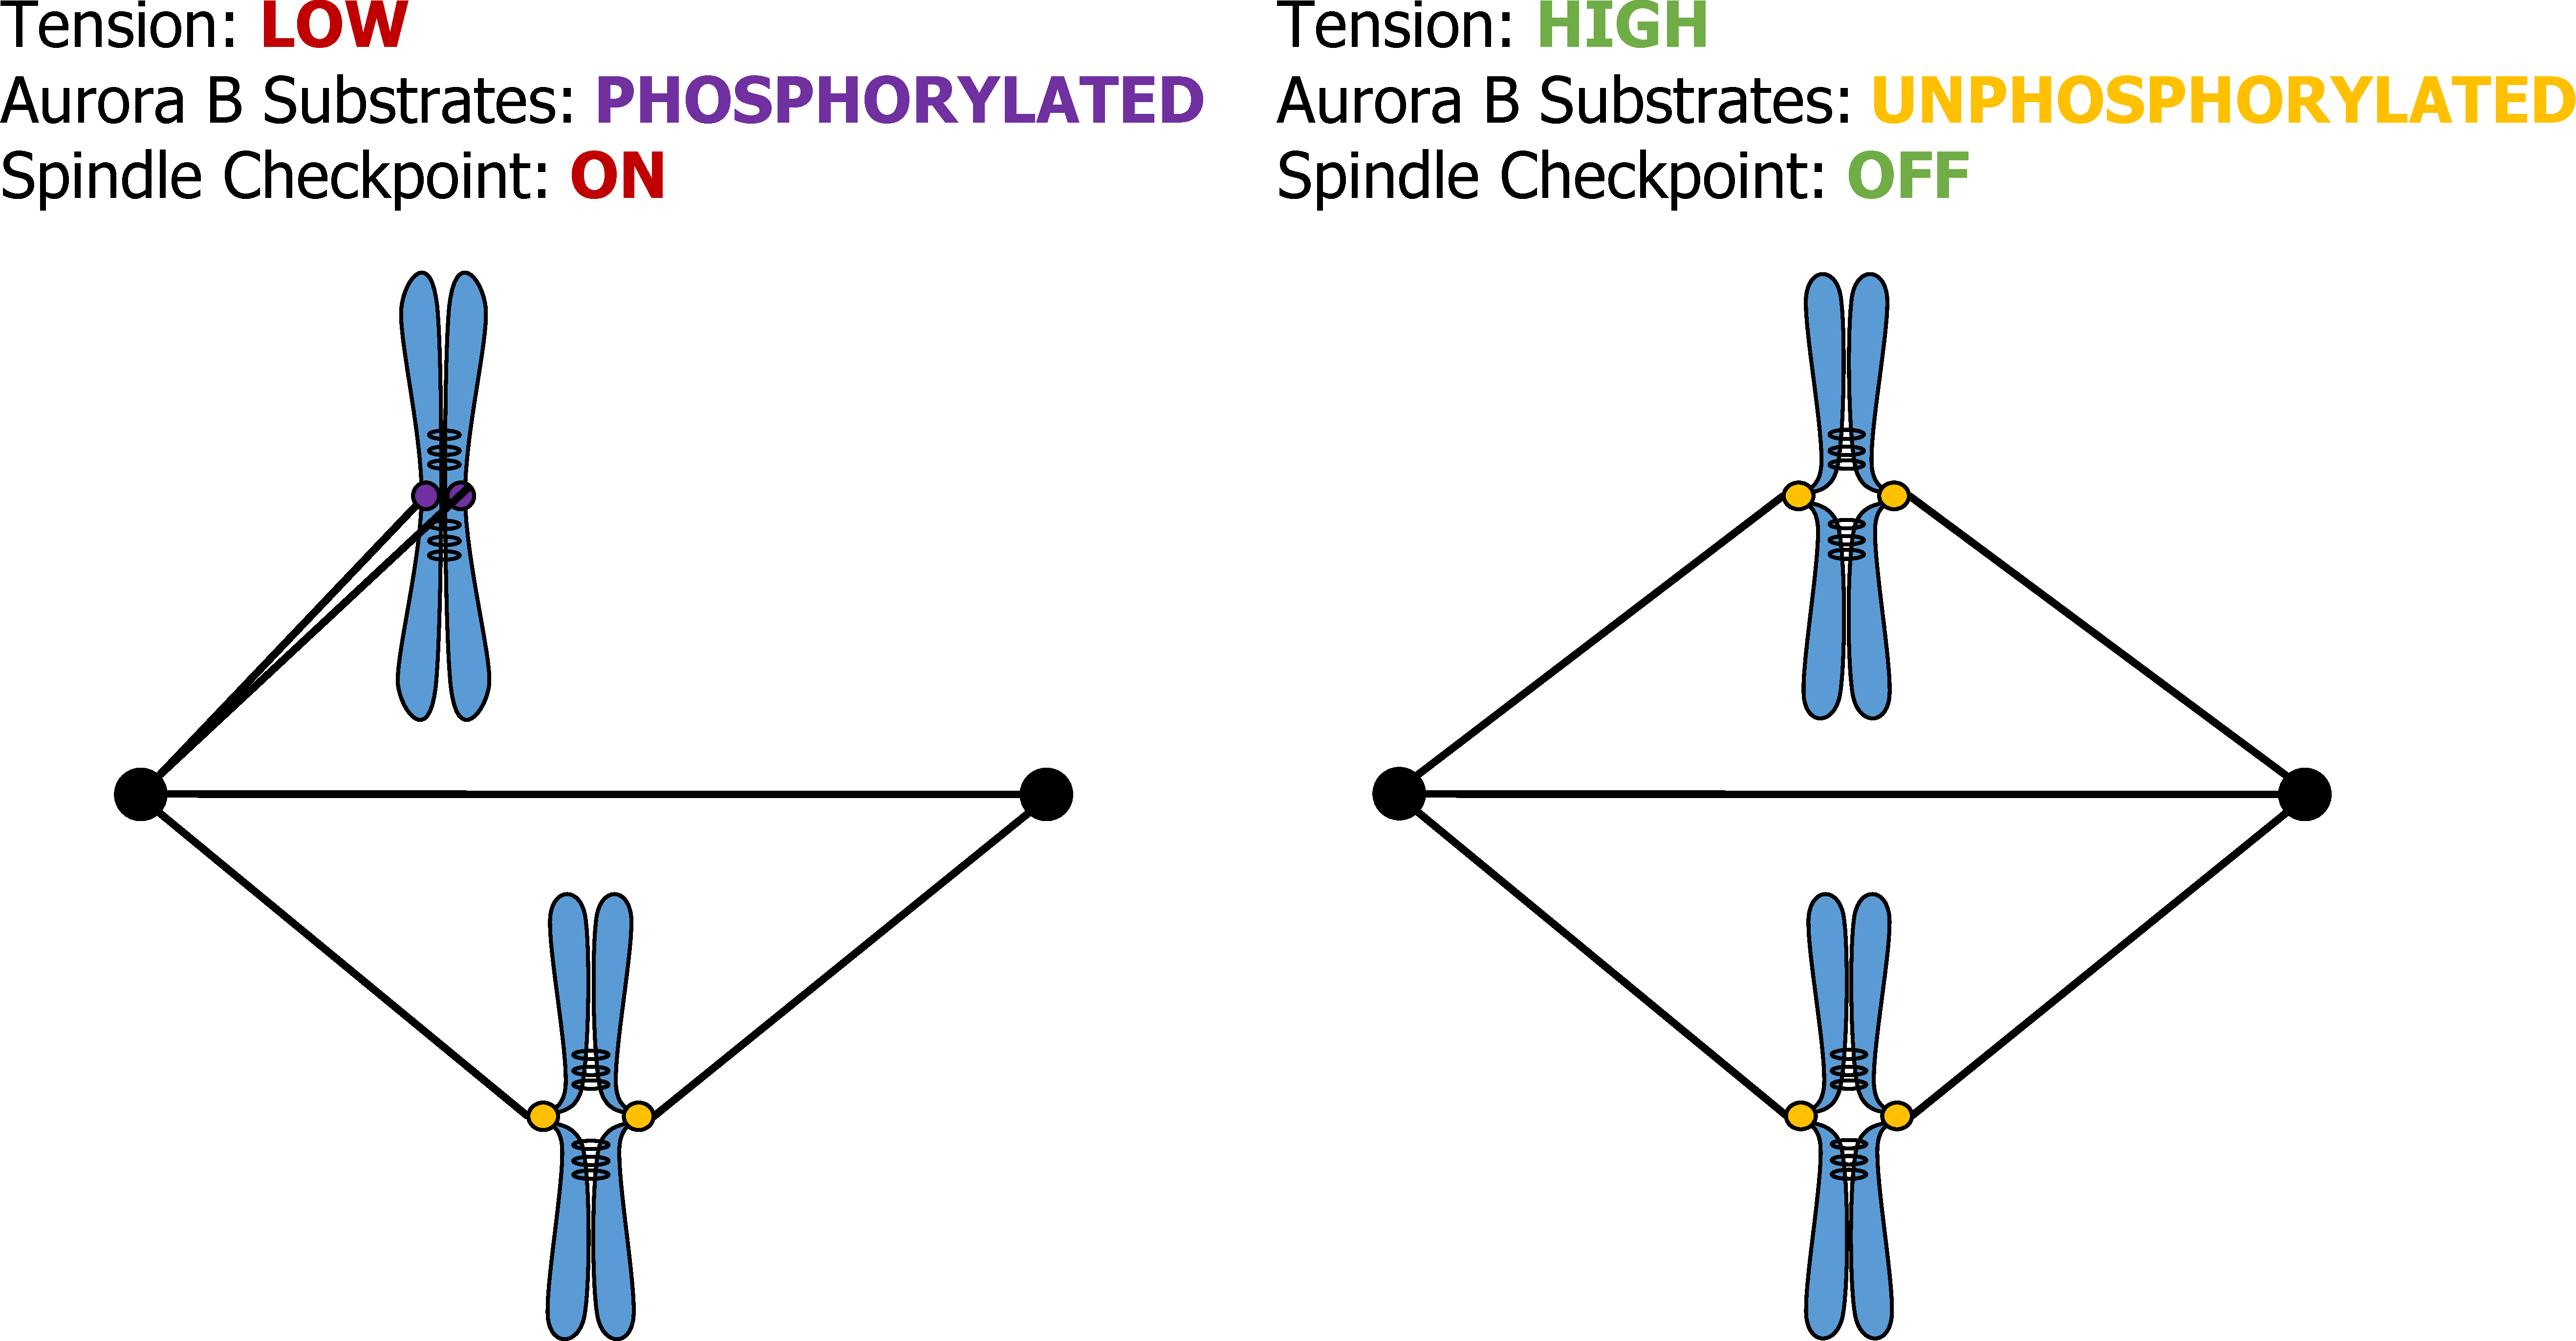
\includegraphics[width=0.9\textwidth]{chapter1/figures/tension sensing schematics.pdf}
  \caption[Tension sensing of the centromere is important for resolving aberrant kinetochore-microtubule attachment]{Tension sensing of the centromere is important for resolving aberrant kinetochore-microtubule attachment. Left: aberrant kinetochore-microtubule attachment is low in tension. The absence of tension triggers the error correction machinery, where the Aurora B kinase phosphorylates kinetochore components to destabilise the erroneous kinetochore-microtubule attachment, enabling new attachment. Error correction can also activate the SAC to prevent anaphase onset by either generating unattached kinetochores or enhancing SAC signalling. Right: Once all pairs of sister chromatids are under tension, The Aurora B substrates are de-phosphorylated. which stabilises the correct kinetochore-microtubule interaction and silences the SAC. }
  \label{fig:tensionSensing}
\end{figure}

\nomenclature{INCENP}{INner CENtromere Protein}
\nomenclature{APC/C}{Anaphase Promoting Complex or Cyclosome}
\nomenclature{ABBA}{cyclin A, BUBR1, BUB1 and Acm1}
\nomenclature{KEN}{lysine(K)-glutamic acid(E)-asparagin(N)}
\nomenclature{CD1}{Conserved Domain 1}

\subsection{Facilitating local cohesion}

Cohesin is the ring-shaped tetramer that is responsible for organising chromosomal architecture \citep{Nasmyth2009Cohesin:Mechanisms, Nasmyth2011Cohesin:Gates, Massari2023ChromosomeATPase}. In mitosis, it is composed of two rod-shaped SMC family members SMC1 and SMC3, the kleisin subunit RAD21 and the associated protein SA1/2. The two SMC proteins bind each other, forming the hinge, and the kleisin RAD21 connects them by their head domains, leading to a ring-like structure for cohesin. Despite that the respective mechanisms are still under active research, cohesin has been found to organise chromosomes by two distinct modes of action, namely extruding intra-molecular loops and generating sister chromatid cohesion. Centromeric cohesion is essential to the establishment of bi-orientation. As mentioned above, bi-orientation is promoted by geometry-induced bias and error correction, both of which require the existence of centromeric cohesion \citep{Tanaka2013}. Indeed, in both vertebrates and yeasts, cohesin is enriched at the peri-centromeric region and the centromere is important for establishing this local cohesion \citep{Tanaka1999IdentificationArms, Blat1999CohesinsRegion, Lengronne2004CohesinTranscription, Laloraya2000ChromosomalMcd1p, Glynn2004Genome-WideCerevisiae}. 

In vertebrates, the centromere concentrates cohesin locally by preventing its removal from the chromatin. Cohesin loaded onto the chromatin can be removed by a WAPL-dependent pathway, called the prophase pathway. In S phase, cohesin is acetylated in the SMC3 subunit and further bound by PDS5, sororin and WAPL \citep{Rankin2005SororinVertebrates, Schmitz2007SororinInterphase, Shintomi2009ReleasingSgo1, Lafont2010SororinCohesion, Nishiyama2010SororinWapl, Song2012CohesinMachinery, Hara2014, Ladurner2016SororinChromatidcohesion}. The association between PDS5 and sororin blocks WAPL from directly interacting with PDS5 \citep{Nishiyama2010SororinWapl, Liu2013}. However, in prophase, mitotic kinases CDK1 and Aurora B phosphorylate multiple sites of sororin, resulting in its disengagement from PDS5 \citep{Rankin2005SororinVertebrates, Shintomi2009ReleasingSgo1, Nishiyama2010SororinWapl, Dreier2011RegulationPhosphorylation, Nishiyama2013AuroraSororin}. WAPL is then able to associate with PDS5, together with the phosphorylation of SA2 by PLK, and promote cohesin removal \citep{Sumara2002TheKinase, Hauf2005DissociationSA2, McGuinness2005ShugoshinCells, Kueng2006WaplChromatin}. At the centromere, the peri-centromeric protein SGO1 antagonises this process by two separate mechanisms. First, SGO1 phosphorylated at T346 competes with WAPL for SA2 and RAD21 binding \citep{Liu2013, Hara2014, Garcia-Nieto2023StructuralProtection}. Second, SGO1 recruits PP2A-B56 to de-phosphorylate SA2 and sororin, causing the re-association of the latter to PDS5 and abolishing WAPL's binding \citep{Kitajima2006a, Tang2006a, Xu2009StructureInteraction, Dreier2011RegulationPhosphorylation, Nishiyama2013AuroraSororin, Hara2014}. As a result, cohesin is spared from the prophase pathway at the centromere and forms local enrichment. 

In yeasts, the centromeric enrichment of cohesin is due to promoted local loading. Cohesin loading is mediated by the SCC2-SCC4 complex, which is hence also called the cohesin loader \citep{Ciosk2000CohesinsProteins, Gillespie2004Scc2Extracts, Watrin2006HumanProgression, Tonkin2004NIPBLSyndrome}. In budding yeast, DDK-dependent phosphorylation of the inner kinetochore component Ctf19 provides a docking site for the cohesin loader Scc2-Scc4 complex, resulting in the targeted loading of cohesin at the centromere \citep{Hinshaw2015StructuralLoading, Hinshaw2017TheComplex, Fernius2009EstablishmentCsm3, Fernius2013Cohesin-DependentEstablishment, Natsume2013KinetochoresRecruitment}. Notably, there is no detectable prophase pathway in budding yeast \citep{Indjeian2005a}. The mechanism is not conserved in fission yeast \citep{PeytonJones2022CohesinPombe}. Although details remain to be elucidated, the peri-centromeric heterochromatin plays an important role. The heterochromatin protein HP1 ortholog Swi6 recruits DDK, which is required for the local enrichment of cohesin \citep{Bailis2003Hsk1Dfp1Centromeres}. The interaction between Swi6 and SA1/2 ortholog Psc3 is also found to be important for this process \citep{Nonaka2001RecruitmentYeast, Bernard2001RequirementCentromeres, Yamagishi2008}. 

\subsection{Initialising chromosome condensation}

In both mitosis and meiosis, the long thin chromosome strands are re-organised into the iconic thick rod-shaped structures exemplified by cell biology textbooks, which is termed chromosome condensation \citep{Antonin2016ChromosomeMitosis, Piskadlo2016NovelCondensation}. It has been proposed to benefit chromosome segregation in various aspects, including spatial compaction, individualisation of sister chromatids and enabling favourable physical properties \citep{Antonin2016ChromosomeMitosis, Piskadlo2016NovelCondensation, Beseda2020MitoticVariability, Takahashi2019FoldingChromosomes}. However, similar to the centromere, despite the cytological and functional appreciation, the form of chromosome condensation (how chromatin is organised in this situation) and how the form achieves the functions still remain elusive. The current model emphasises two distinct pathways for chromosome condensation, with one being the looping of DNA strands mediated by condensin and the other being the intrinsic attraction between nucleosomes regulated by histone PTMs. \cite{Kruitwagen2015a} defined the former as 'compaction' and the latter as 'contraction'. Emerging evidence points to a positive role of the centromere in both pathways of chromosome condensation, suggesting a novel way by which the centromere facilitates accurate chromosome segregation \citep{Leonard2015, Wilkins2014AMitosis, Kruitwagen2018, Hendzel1997Mitosis-specificCondensation, Oliveira2007CondensinChromosomes, Chan2004CondensinDivisions, Hagstrom2002C.Meiosis, Maddox2006MolecularAssay, Maddox2007FunctionalChromatin, Wenda2021MitoticElegans}. 

Condensin is the pentameric protein complex composed of two SMC subunits, SMC2 and SMC4, and three auxiliary subunits, CAP-D2/3, CAP-G/2 and CAP-H/2 \citep{Hirano2012Condensins:Functions, Kalitsis2017CondensinGenome}. It is highly conserved and structurally similar to the cohesin complex \citep{Davidson2021GenomeComplexes}. SMC2 and SMC4 interact at one end called the hinge and their other ends called the heads are linked by the kleisin subunit CAP-H/H2, forming a ring-like structure. This structural similarity brings the possibility that condensin might entrap DNA as cohesin does, which is supported by the evidence from budding yeast \citep{Cuylen2011CondensinLinks, Ganji2018Real-timeCondensin}. The role of condensin in chromosome condensation is discovered because its depletion resulted in a delay in the process \citep{Hagstrom2002C.Meiosis, Kaitna2002TheMeiosis, Hudson2003CondensinChromosomes}. The mechanism of action is unclear but it is known that condensin is capable of introducing positive supercoils of DNA \citep{Hirano2012Condensins:Functions}. It has also been speculated that condensin could multimerise, evidenced by that multiple \textit{Escherichia coli}'s SMC proteins aggregated in proximity under the microscope \citep{Badrinarayanan2012InProteins} and that condensin complexes purified from chicken \textit{Gallus gallus} DT40 cells showed populations with different molecular weights \citep{Barysz2015Three-dimensionalModelling}. The multimerisation of condensin is suggested to give rise to higher-order structures of chromatin, such as the flower petal structure, further facilitating chromosome condensation \citep{Piskadlo2016NovelCondensation, Kalitsis2017CondensinGenome}. 

The notion that there exist non-condensin-mediated chromosome condensation pathways came from the observation that depletion of condensin did not completely, if at all, abolish chromosome condensation \citep{Hudson1998CentromereWeights, Gerlich2006CondensinCells, Vagnarelli2006CondensinMitosisb, Kireeva2004VisualizationStructure, Hagstrom2002C.Meiosis}. A series of evidence implicated that inter-nucleosomal interactions might be the alternative to condensin, which is under the regulation of a cascade of histone modifications. It is well characterised by \textit{in vitro} experiments that the acid patch of H2A-H2B could attract the H4 tail from another nucleosome \citep{Robinson200830nmEviction, Shogren-Knaak2006HistoneInteractions}. Subsequent work from budding yeast \citep{Wilkins2014AMitosis, Kruitwagen2015a} indicated that the acetylation of H4-K16 inhibits this interaction. In mitosis, the phosphorylation of H3-T3 by Haspin kinase recruits the CPC to further phosphorylate H3-S10. The latter is then read by the de-acetylase Hst2, which removes H4-K16ac to enable the intrinsic interaction between H4 and neighbouring H2A-H2B. 

Centromere has been indicated to regulate chromosome condensation. Defected chromosome condensation was observed when the holo-centromere of \textit{C. elegan} was disrupted by depleting CENP-A or the loader KNL-2 \citep{Chan2004CondensinDivisions, Maddox2006MolecularAssay, Hagstrom2002C.Meiosis, Maddox2007FunctionalChromatin}. In line with this, the chromatin level of condensin II was further found to depend on KNL-2 \citep{Wenda2021MitoticElegans}. In regional and point centromere species, chromosome condensation is suggested to be initialised at the centromere and then propagated to the chromosome arms \citep{Kruitwagen2018}. H3-pS10, the contraction indicator, was found to localise at the centromere initially and then spread to the rest of the genome at a similar pace with chromosome condensation in Indian muntjac \textit{Muntiacus muntjak} \citep{Hendzel1997Mitosis-specificCondensation}. Whereas in \textit{D. melanogaster} and budding yeast, it is the compaction that was found to propagate, where condensin was first detected at the centromere and then the distant loci \citep{Oliveira2007CondensinChromosomes, Leonard2015}. \cite{Kruitwagen2018} further found in budding yeast that chromosome condensation is regulated by the centromere autonomously in a CPC-dependent manner and that its propagation requires signalling cascades involving Sgo1 and Hst2. Thus, the centromere might contribute to chromosome condensation via both compaction and contraction. 

\section{Aims of the study}

The spatial organisation and dynamics of proteins are common practices that biological systems employ to dramatically increase their complexity given a certain amount of genetic information, which enables the remarkable richness of behaviours required to meet the tough challenges they face. There is no exception for the centromere, where its function of ensuring accurate chromosome segregation is partially, if not primarily, realised by regulating the spatial organisation of critical proteins. Mechanistic explanations for many of these fascinating processes are still lacking. In this work, we chose to study the mechanisms behind the spatial organisation and dynamics of two key centromeric proteins, CENP-A and Shugoshin, with a wishful ambition that they might be interrelated and cooperatively contribute to our understanding of tension sensing. 

\subsection{Building a theoretical model for the spatial organisation of CENP-A nucleosomes}

The identity of a centromere is determined epigenetically by the presence of nucleosomes containing the H3 variant CENP-A \citep{Warburton1997ImmunolocalizationCentromeres, Vafa1997ChromatinPlate, Earnshaw1985ThreeChromosome, Liu2006MappingCells, Regnier2005CENP-ABubR1, Heun2006, Mendiburo2011, Barnhart2011, Logsdon2015, Logsdon2019}. A qualitative model has emerged from experimental data that the propagation of CENP-A nucleosomes mainly depends on a self-templating positive feedback loop involving CENP-C, MIS18 complex and CENP-A nucleosome chaperon HJURP \citep{McKinley2015, Stirpe2022}. Nevertheless, it fails to explain a list of interesting phenomena of CENP-A spatial organisation. The centromere shows around 50-fold higher enrichment of CENP-A nucleosomes over chromosome arms \citep{Bodor2014}. It is not known what causes the difference. Despite the relative enrichment, the proportion of CENP-A nucleosomes to total nucleosomes is surprisingly low at the centromere \citep{Bodor2014, Schittenhelm2010}. How is homeostasis maintained at such a low value remains unclear. Moreover, the spatial pattern of CENP-A nucleosomes at the centromere is non-random, where small clusters of CENP-A nucleosomes are found to be interspersed with canonical H3 nucleosomes \citep{Blower2002ConservedHumans, Dunleavy2011H3.3Phase., Kyriacou2018}. How this pattern is formed is beyond the territory of the current paradigm. Compared to experimental approaches, theoretical deduction possesses advantages in uncovering the basic principles behind observations due to rigorous mathematical expression \citep{Fidelman1985TheModeling}. Thus, we decided to build a theoretical model for the spatial organisation of CENP-A nucleosomes on chromatin, attempting to answer these questions. 

\subsection{Investigating the molecular mechanisms underlying the tension-dependent re-localisation of Shugoshin}

Shugoshin is a peri-centromeric adaptor protein crucial for accurate chromosome segregation \citep{Marston2015, Zhang2020FunctioningMitosis}. Interestingly, it exhibits rich dynamics in terms of spatial organisation in various species, where the localisation is dependent on tension, a mechanical force \citep{Huang2007, Lee2008, Liu2013, Asai2020, Lee2008, Gomez2007, Eshleman2014, Nerusheva2014, Paldi2020ConvergentPericentromeres, Clarke2005, Kawashima2007}. This re-localisation has been implicated to participate in important cellular processes, such as cohesin de-protection, tension sensing and potentially chromosome condensation \citep{Indjeian2005a, Nerusheva2014, Su2021SumoylationAnaphase, Lee2008, Liu2013, Leonard2015, Kruitwagen2018}. Abolishing such re-localisation caused a delay in cell cycle progression and errors in chromosome segregation \citep{Su2021SumoylationAnaphase, Liu2013}. However, the underlying molecular mechanisms are still elusive. Hence, we aimed to construct a qualitative model for the tension-dependent re-localisation of Shugoshin using experimental approaches. We chose to use the model organism budding yeast for its unique advantages specific to this topic. A budding yeast kinetochore can only bear a single microtubule \citep{Biggins2013TheKinetochore}. This benefits research involving tension in that complicated kinetochore-microtubule attachment modes such as merotelic attachment are excluded, resulting in a straightforward interpretation of results \citep{Tanaka2010Kinetochore-microtubuleBi-orientation}. Moreover, unlike mammals, budding yeast encodes only one Shugoshin variant \textit{SGO1} \citep{Marston2015}, which further simplifies the question. 

\subsection{Exploring the potential link between the chromatinic pattern of CENP-A nucleosomes and tension sensing}

The concept that tension is the clue for the bi-orientation of sister chromatids sensed by cells has been established for over 60 years. The phosphorylation statuses of Aurora B substrates at the kinetochore have been recognised as the readout for tension sensing. However, the key question 'How does tension regulate these phosphorylations?', or the plain language version 'How is tension sensed?' has been troubling the field. A number of models that are neither mutually exclusive nor can be easily proven with current experimental techniques have been proposed \citep{McVey2021AuroraSegregation}. Among them, one model has gained particular popularity, where the CPC is physically separated from its kinetochore substrates in response to tension due to altered localisation. The CPC is localised to the inner centromere during prometaphase and metaphase. Although there exists controversy, two distinct recruitment arms are believed to determine this localisation, one being through the binding of Survivin to the phosphorylation of H3-T3 by the Haspin kinase while the other one being through multipartite interactions between CPC subunits and SGO1 recruited by the phosphorylation H2A-T120 by BUB1 \citep{Abad2022MechanisticCPC}. The tension-dependent re-localisation of shugoshin provides a possible explanation for how the localisation of the CPC could respond to tension \citep{Nerusheva2014}. This reasoning is supported by the experimental data from budding yeast that \textit{sgo1} mutants failed to conduct error correction, which implied the incapability of tension sensing \citep{Indjeian2005a}. 

Form follows function. Tension sensing must be enabled by the unique properties of the centromere. The non-random distribution of CENP-A nucleosomes might underlie them. The point centromere species budding yeast has only one CENP-A nucleosome per chromosome \citep{Biggins2013TheKinetochore}. The kinetochore assembled by it loads cohesin \textit{in cis} to organise the peri-centromeric chromatin into special conformations, which is important for Sgo1's chromatin localisation and faithful chromosome segregation \citep{Paldi2020ConvergentPericentromeres, Fernius2009EstablishmentCsm3, Fernius2013Cohesin-DependentEstablishment, Hinshaw2015StructuralLoading, Hinshaw2017TheComplex, Natsume2013KinetochoresRecruitment}. The current view of the kinetochore of a regional centromere species holds that it is composed of multiple copies of the unit module equivalent to a budding yeast kinetochore \citep{Walstein2021}. It is possible that, in higher eukaryotes, the distinct islands of CENP-A nucleosomes are responsible for the assembly of individual unit modules of the kinetochore, shaping the conformation of surrounding chromatin. This spatial structure might be required to localise Shuogoshins properly and provide special mechanical properties. Shugoshins are thus prepared for their tension-dependent re-localisation to facilitate tension sensing as described above. Therefore, this work also aimed to explore the potential link between the chromatinic pattern of CENP-A nucleosomes and tension sensing. 
% \chapter{Building a theoretical model for the dynamics and self-organization of centromeres}

\section{Introduction}

The centromere identity is epigenetically determined by the histone H3 variant CENP-A in organisms with regional centromeres \citep{Warburton1997ImmunolocalizationCentromeres, Vafa1997ChromatinPlate, Earnshaw1985ThreeChromosome, Liu2006MappingCells, Regnier2005CENP-ABubR1, Heun2006, Mendiburo2011, Barnhart2011, Logsdon2015}. Contrary to the epigenetic nature, the chromosomal position of a centromere is inherited over generations of cells with astonishing fidelity and only changes if viewed from an evolutionary timescale \citep{Amor2004HumanProgress, Murphy2005DynamicsMaps}. This implies the existence of strategies ensuring the propagation, maintenance and specificity of CENP-A at centromeres. Indeed, various delicate molecular mechanisms conserved across species have been found. 

DNA replication during the S phase inevitably dilutes the number of CENP-A nucleosomes in one chromosome at least by half, where full conservation of old CENP-A is assumed. Therefore, the propagation of CENP-A nucleosomes over generations relies on the deposition of new CENP-A into the chromatin. A conserved positive feedback mechanism has emerged across different species, where old CENP-A is read by proteins that can recruit the CENP-A specific chaperon to deposit new CENP-A \citep{Stirpe2022, McKinley2015}. In vertebrates, CENP-A binds the CCAN protein CENP-C and together they recruit the Mis18 complex, consisting of Mis18$\alpha$, Mis18$\beta$ and Mis18BP1 \citep{Westhorpe2015AMaintenance, Moree2011CENP-CAssembly, Dambacher2012CENP-CChromatin, French2017XenopusAssembly, Wang2014MitoticHJURP, Pan2019MechanismLicensing}. The CENP-A chaperon HJURP bearing CENP-A-H4 heterodimer is then targeted to the centromere by the Mis18 complex \citep{Foltz2009, Dunleavy2009}. CENP-B, the centromeric protein that binds the 17-bp DNA motif CENP-B box, is reported to reinforce this process by stabilising CENP-C \citep{Fachinetti2015, Hoffmann2020, Chardon2022CENP-B-mediatedCentromeres, Masumoto1989ASatellite., Suzuki2004CENP-BLocalization} and is believed to be the 'safety net' for the positive feedback loop \citep{Berg2020}. Similarly, in fission yeast, its Mis18 complex, composed of Mis16, Mis18 and Eic1, and the CENP-A chaperon Scm3 are required for the assembly of its CENP-A ortholog Cnp1 at the centromere \citep{Pidoux2009FissionChromatin, Hayashi2004Mis16Centromeres, Williams2009FissionChromatin}, albeit the requirement for Cnp3, the fission yeast CENP-C, is not conserved \citep{Subramanian2014Eic1Assembly}. Mis18 complex and HJURP orthologs are not found in \textit{Drosophila}. But their functions are combined in one single protein CAL1, which possesses the CENP-A chaperon activity and can self-target to the centromere by interacting with CENP-C and \textit{Drosophila} CENP-A CID \citep{Chen2014, MedinaPritchard2020, Phansalkar2012EvolutionaryDrosophila, Roure2019, Schittenhelm2010}. Additional factors are required for CID deposition in this system, including the FACT complex \citep{Chen2015EstablishmentTranscription} and CAF1 \citep{Furuyama2006Chaperone-mediatedVitro, Boltengagen2016AMelanogaster}. Even in point centromere species budding yeast, whose centromeres are determined genetically, this mechanism is partially conserved. The CBF3 complex recognises the centromeric sequence CDEIII and recruits the chaperon Scm3 to deposit the CENP-A ortholog Cse4 \citep{Camahort2007Scm3Kinetochore, Guan2021StructuralFormation, Cho2011Ndc10Yeast, Mizuguchi2007NonhistoneNucleosomes, Zhou2011StructuralScm3, Meluh1998Cse4pCerevisiae}. Although the exact timing might range from late M to early G1 phase, a common feature of CENP-A deposition shared by various species is that it happens outside the S phase, unlike canonical histone proteins \citep{Fukagawa2014, McKinley2015TheFunction, Stirpe2022}. Consistent with this feature, in vertebrates, the centromeric localisation of HJURP and Mis18BP1 is prevented by CDK1/2-dependent phosphorylation, whose activity is elevated in mitosis and reduced in interphase \citep{Silva2012, Spiller2017MolecularDeposition, Stankovic2017}. The deposition machinery is further regulated by PLK1, which phosphorylates Mis18BP1 and promotes its localisation to the centromere \citep{McKinley2014Polo-likeCentromeres}. Apart from the positive feedback loop and phospho-regulation, proper deposition of CENP-A requires centromeric transcription \citep{Bergmann2012EpigeneticFunction, Catania2015SequenceChromatin, Cardinale2009HierarchicalModifier, Choi2011IdentificationCentromeres, Nakano2008InactivationModifiers, Zhu2018HistoneChromosomes}. It is reasoned that transcription facilitates new CENP-A deposition by evicting embedded non-CENP-A nucleosomes \citep{Chen2015EstablishmentTranscription, Choi2011IdentificationCentromeres, Bobkov2018, Bergmann2012EpigeneticFunction, Bobkov2020, Choi2017TheH3, Prasad2011NewCentromeres}. 

Similar to other epigenetic marks, the maintenance of CENP-A nucleosomes is challenged by chromatin remodelling activities such as replication and transcription. Yet, CENP-A possesses unusual stability that it does not turn over once incorporated into the chromatin \citep{Falk2015, Jansen2007, Bodor2013, Smoak2016Long-TermIdentity}. In replication, this has been attributed to the recycling of disrupted CENP-A-H4 heterodimer by HJURP interacting with MCM2 of the replication fork \citep{Zasadzinska2018, Zasadzinska2013DimerizationDeposition, Huang2015AForks} in a similar manner to the retention of canonical H3 by Asf1$\alpha$ \citep{Richet2015StructuralFork, Clement2015MCM2Fork}. This resulted in the conservative partition of existing CENP-A nucleosomes between the newly replicated sister chromatids \citep{Falk2015, Jansen2007, Bodor2013}. Due to the temporal separation of replicative dilution and new CENP-A deposition, the gaps generated are then filled by another histone H3 variant H3.3 as the placeholder \citep{Dunleavy2011H3.3Phase.}. As mentioned above, transcription can lead to the eviction of incorporated nucleosomes. The general chaperon FACT complex and Spt6 have been proposed to travel with RNA Pol II and reassemble CENP-A nucleosomes dissembled due to transcription \citep{Bobkov2020, Jeronimo2019HistoneModifications, Kato2013Spt6H3, Boltengagen2016AMelanogaster}.

Counter-intuitively, the majority of CENP-A nucleosomes are localised on chromosome arms \citep{Bodor2014}. This could be due to the random deposition of CENP-A caused by the large quantity and the promiscuity to general histone chaperons. Nevertheless, the centromeric enrichment is still over 50-fold higher than arms \citep{Bodor2014}. Apart from the isolation of CENP-A deposition from canonical histone proteins mentioned above, nucleosome eviction by replication, gene expression regulation and PTMs are used to improve the specificity of CENP-A at the centromere. Replication is the main mechanism to remove ectopic CENP-A nucleosomes \citep{Nechemia-Arbely2019, Wang2021PhosphorylationCycle}, with the centromeric ones being proposed to be protected by the CCAN \citep{Nechemia-Arbely2019}. In human and fission yeast cells, CENP-A transcription coincides with their respective deposition timings \citep{Shelby1997AssemblySites, Takahashi2000RequirementYeast, Aristizabal-Corrales2019CellFormation}. Moreover, it has been observed that the expression of CENP-A outside the normal time window would lead to ectopic incorporation in different organisms \citep{Aristizabal-Corrales2019CellFormation, Heun2006, Tomonaga2005CentromereAneuploidy, Au2008AlteredCerevisiae, Olszak2011, McGovern2012CentromereCancer, Athwal2015CENP-ACells, Shrestha2021, Moreno-Moreno2019TheCycle}. Among the various  PTM-based mechanisms for regulating CENP-A localisation, ubiquitin-mediated protein degradation is the most common one \citep{Stirpe2022}. In human \citep{Maehara2010CENP-AMitoses, Lomonte2001DegradationICP0}, \textit{Drosophila} \citep{Moreno-Moreno2019TheCycle, Bade2014TheManner} and budding yeast \citep{Ranjitkar2010AnDomain, Au2013AProteolysis, Mishra2015Pat1Ubiquitination, Zhou2021MolecularPsh1} cells, ubiquitination has been reported to remove CENP-A outside the centromeric regions. 

Despite that extensive studies have been conducted on the molecular biology of centromere specification and propagation, our understanding of the system is compromised due to the absence of a mechanistic mathematical model. The different enrichment of CENP-A nucleosomes at centromeres and arms implicated the existence of two stable equilibrium states, or bi-stability, in the system. Positive feedback is known for its capability to generate bi-stability in biological systems \citep{Mitrophanov2008PositiveSystems, Ferrell2013FeedbackCycle}. It is tempting to hypothesise that the molecular mechanism of CENP-A deposition is sufficient to explain the difference in enrichment between centromeres and arms. Yet, the signal amplifier, or 'all or nothing', nature of positive feedback loops contrasts the low density of CENP-A nucleosomes at centromeres, where they only account for about 1 in 25 nucleosomes \citep{Bodor2014, Schittenhelm2010}. CENP-A further possesses intriguing features in terms of spatial localisation on the chromatin. Rather than distributed homogeneously, the CENP-A nucleosomes are visualised as distinct clusters on an extended chromatin fibre \citep{Blower2002ConservedHumans, Dunleavy2011H3.3Phase., Kyriacou2018}. It would be interesting to understand the mechanism behind this pattern formation. Therefore, this project aims to build a theoretical model describing the dynamics and spatial patterns of CENP-A, with the expectation to recapitulate the key characteristics of the system, including bi-stability, low density at the higher steady state and the maintenance of island patterns. 

\nomenclature{CENP-A}{CENtromere Protein A}
\nomenclature{CCAN}{Constitutive Centromere Associated Network}
\nomenclature{HJURP}{Holliday JUnction Recognition Protein}
\nomenclature{CID}{Centromere IDentifier}
\nomenclature{FACT}{Facilitates Chromatin TranscripTion}
 
\section{Methods}
\subsection{The model}

Inspired by the classic theoretical model for epigenetics \citep{Dodd2007, Micheelsen2010TheoryLandscapes}, we decided to use a CA-like, 1D, rule-based stochastic model for the CENP-A system. As a starting point, we developed a basic model, where the molecular knowledge of CENP-A propagation and maintenance is described in its simplest manner. The assumptions used for the basic model are as follows: 

(1) A certain number of sequentially placed nucleosomes composed of either canonical H3 or CENP-A nucleosomes was considered to represent the centromere. Because the lengths of centromeres vary largely among species and even between different chromosomes in the same species, we did not set a fixed value for the number of nucleosomes. As will be shown in the later section, this variable only provides a minor effect on the model's behaviours. Periodic boundary conditions were used to avoid potential artefacts from boundaries. 

(2) At each time step, CENP-A nucleosomes are first replenished and then diluted (Figure~\ref{fig:basicmodelschematics}B). This is because CENP-A is deposited at the interphase while diluted at the S phase in most species. The two processes will be referred to as 'replenishment' and 'dilution' in the following texts for convenience. We assume no loss of CENP-A except replicative dilution as the ultra-low turnover rate of CENP-A nucleosomes mentioned above. 

(3) For replenishment, H3 nucleosomes were converted to CENP-A nucleosomes because of pre-existing CNEP-A nucleosomes in proximity (Figure~\ref{fig:basicmodelschematics}A). Notably, the positive feedback of CENP-A deposition was simplified as its local self-promoting property in this case. The detailed algorithm of this process will be described in the following implementation sub-section. 

(4) For dilution, CENP-A nucleosomes were assumed to be randomly distributed to daughter centromeres as observed in wet-lab experiments (Figure~\ref{fig:basicmodelschematics}A). 

\begin{figure}[htbp]
  \centering
  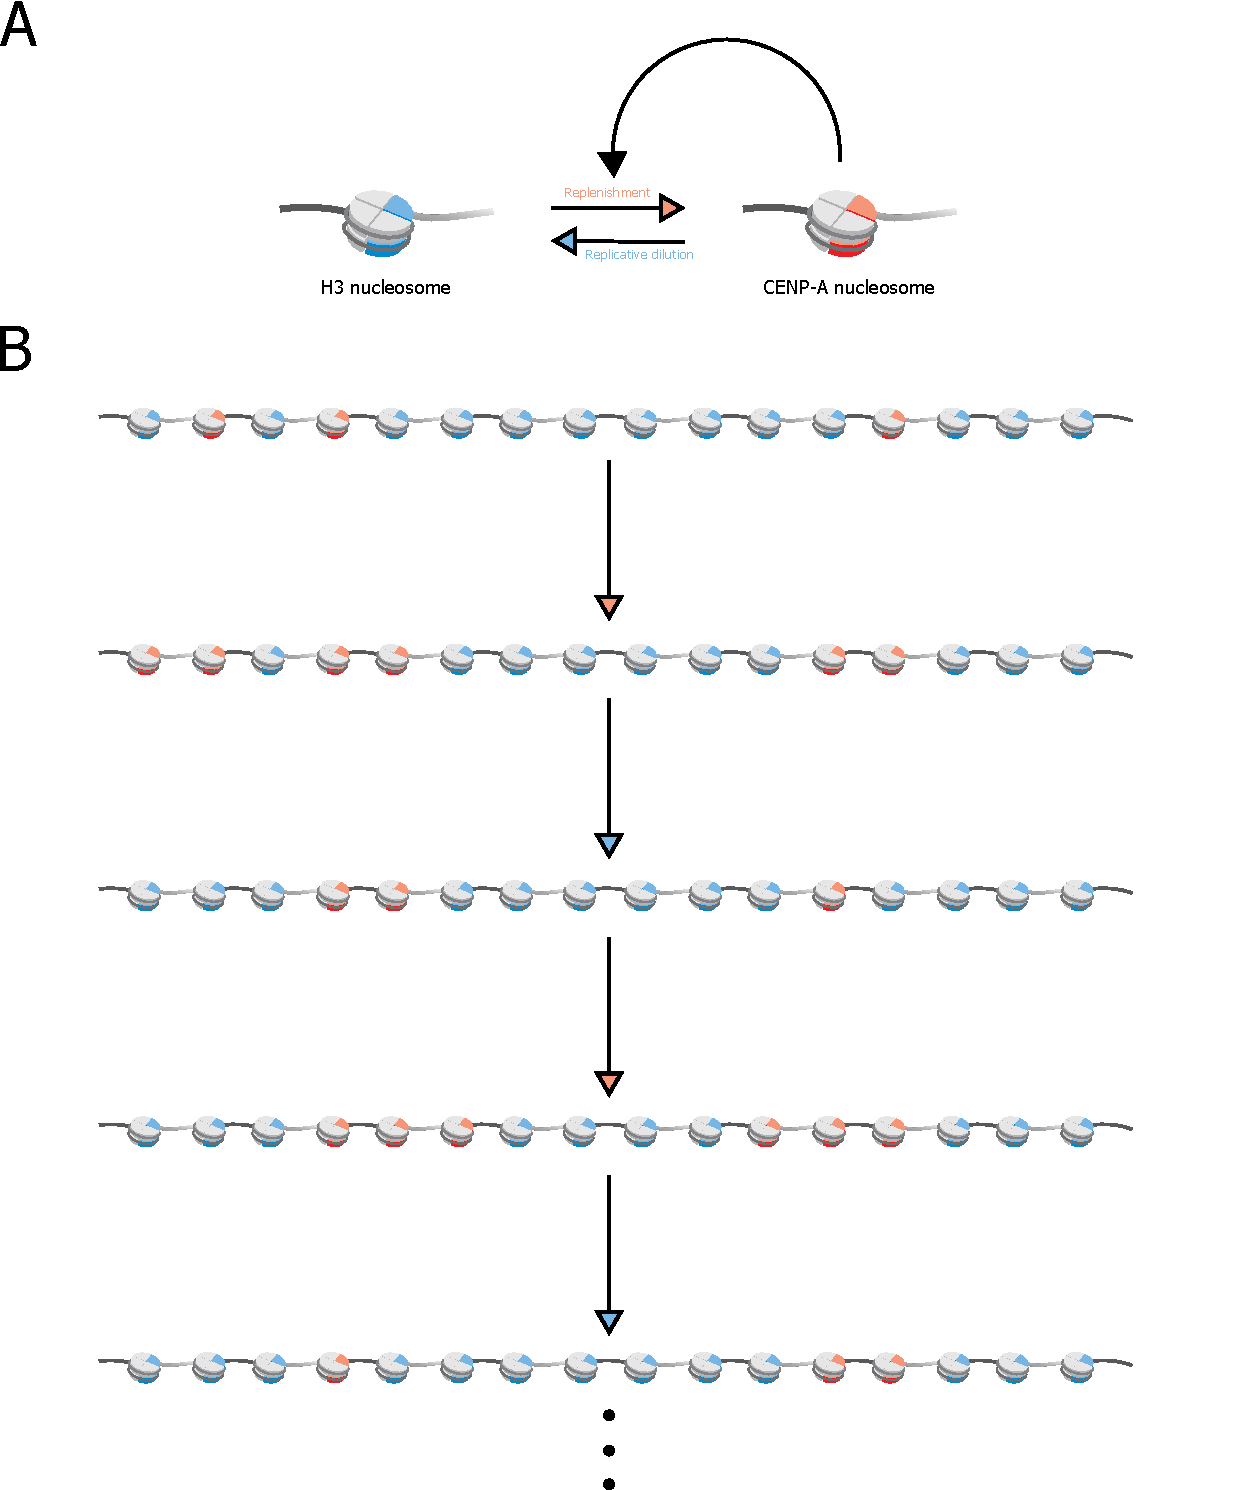
\includegraphics[width=0.9\textwidth]{chapter2/figures/the model.pdf}
  \caption[Schematics of the basic model]{Schematics of the basic model. (A) Schematics of the interchange between CENP-A and H3 nucleosomes. CENP-A nucleosomes are converted to H3 nucleosomes due to replicative dilution. H3 nucleosomes are converted to CENP-A nucleosomes by replenishment, where pre-existing CENP-A nucleosome facilitates the conversion of H3 nucleosomes locally. (B) An example of the evolution of the basic model. The array of nucleosomes undergoes replenishment and dilution at each cell cycle. }
  \label{fig:basicmodelschematics}
\end{figure}

\nomenclature{CA}{Cellular Automata}
\nomenclature{1D}{one-Dimensional}

\subsection{Implementation}

The model describes the centromere as a 1D array of a certain number, denoted by $NN$, of cells with two states, either 1, representing the CENP-A nucleosome or 0, representing the H3 nucleosome.

\subsubsection{Initialisation}

To unbiasedly initialize such an array, a stochastic approach is used. a 1D array of 0 was first created. Each 0 in the array then has a probability of the arbitrary initial CENP-A density, denoted by $\rho_{0}$, to be converted to 1. A typical array was exemplified in Figure~\ref{fig:array}. The density and spatial pattern of CENP-A are used as read-outs of the state of the  array. Density is calculated by dividing the sum of the array, which equals the number of 1s in the array, by the length of the array. As a mimicry of CENP-A imaging data from biological experiments, spatial pattern is visualized by plotting the array with 1 as white and 0 as black. \\

\begin{figure}[htbp]
  \centering
  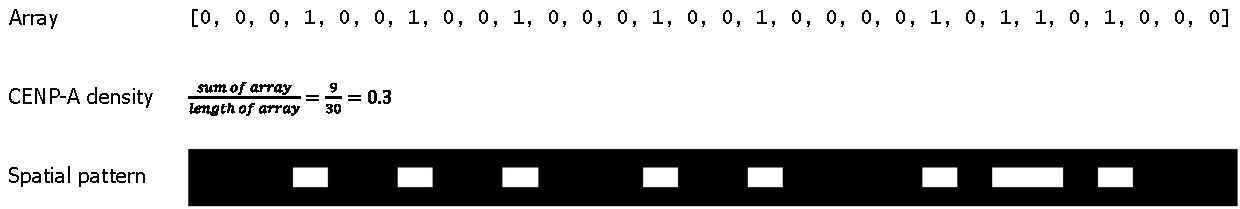
\includegraphics[width=0.9\textwidth]{chapter2/figures/the array.pdf}
  \caption[The implementation of the basic model]{The implementation of the basic model. The centromere is described as a finite 1D array composed of only 0 and 1, with 0 representing the H3 nucleosome and 1 representing the CENP-A nucleosome. The density of CENP-A is calculated by dividing the sum of the array by the length, or the number of cells, of the array. The spatial pattern of CENP-A distribution is visualised by colouring 1 as white and 0 as black. }
  \label{fig:array}
\end{figure}

\subsubsection{Replenishment}

As with other CA models, our model updates the state of a cell by a state-transition function that reads the states of neighbour cells. To describe the replenishment, where new CENP-A nucleosomes replace H3 nucleosomes due to pre-existing CENP-A and the CENP-A nucleosomes do not turn over, we set the state-transition function as such: 
\begin{align*}
    & P_{0\rightarrow 1}=\alpha\sum_{i=-n}^{n} x_if_i \\
    & P_{1\rightarrow 0}=0 
\end{align*}
where $\alpha$ is an arbitrary parameter denoting the loading efficiency, $n$ denotes the size of the neighbourhood, $x$ is the state of the cell $i$ and $f$ is the weight function, which is a Gaussian function with a mean of 0 and a standard deviation of n/3 ($f\sim Gaussian(\mu=0, \sigma=\frac{n}{3}$) used to model the assumption that the probability of interaction decreases with physical distance. 

To enable more flexibility of replenishment, we allowed it to happen multiple rounds before dilution. The number of rounds was denoted by $rr$. 

\subsubsection{Dilution}

Ideally, one array should be divided into two daughter arrays during each dilution event. Yet, the number of arrays would grow exponentially with the simulation steps, as would the computational time required. To simulate the evolution of the array for more steps, only one of the daughter arrays was tracked. Hence, replicative dilution is modelled by the process where each 1 in the array has a probability of 0.5 to be converted to 0, which leads to the following state-transition function: 
\begin{align*}
    & P_{0\rightarrow 1}=0 \\
    & P_{1\rightarrow 0}=0.5
\end{align*}
The parameters of the basic model were summarised in Table~\ref{tab:parameters}. \\

\begin{table}[htbp]
\centering
\caption{The parameters of the basic model}
\label{tab:parameters}
\begin{tabular}{cl}
\hline
\textbf{Parameters} & \multicolumn{1}{c}{\textbf{Description}} \\ \hline
$NN$                  & The number of nucleosomes                \\
$\rho_{0}$               & The initial density of CENP-A            \\
$\alpha$               & The  loading efficiency                  \\
$n$                   & The size of neighbourhood                \\
$rr$                  & The number of replenishment rounds      \\ \hline
\end{tabular}
\end{table}

\section{Results}
\subsection{The basic model exhibits two types of behaviour}

We started by experimenting with different combinations of parameters and classifying behaviours of the basic model based on CENP-A density evolution maps (Figure~\ref{fig:modelBehaviour}A and B left). A density evolution map presents how CENP-A density changes over time. In general, two types of behaviour were observed. First, the density eventually
reaches 0 (Figure~\ref{fig:modelBehaviour}A). Due to the fact that new CENP-A nucleosomes require old CENP-A nucleosomes to be recruited, once the density reaches 0, it will stay at 0. We named this type of behaviour ‘dead’. The second type is where CENP-A density is fluctuating around a value less than 0.5 after a number of generations (Figure~\ref{fig:modelBehaviour}B). We called this type of behaviour ‘stabilized’. The maximal value of density cannot be greater than 0.5 because we update the array by first replenishing and then diluting it. Then we sought to visualise the evolution of the CENP-A spatial pattern of the two behaviours by stacking spatial patterns according to generation. We termed this plot spatial pattern kymograph (Figure~\ref{fig:modelBehaviour}A and B right). For the ‘dead’ type behaviour, CENP-A nucleosomes formed inheritable aggregates, or islands, which could diverge or be combined. But all the islands vanished eventually. For the ‘stabilized’ behaviour, the islands could be seen in the first several time steps. After that, the islands joined each other and formed random-like distribution of CENP-A. Given the auto-amplification property of CENP-A deposition, the existence of ‘stabilized’ behaviours, where CENP-A density can be stabilised before saturation, is surprising. We reasoned that this is because as the density of CENP-A nucleosome increases, the number of H3 nucleosomes decreases, leading to a reduced room for new CENP-A to be deposited. This counteracts auto-amplification and results in a steady state. 

We next attempted to systematically view how model behaviours change with parameters. Due to the predictable positive effect on the CENP-A density of $rr$, I fixed it and ran simulations with different combinations of the loading efficiency $\alpha$ ranging from 0 to 1 with a step size of 0.02 and the range of local deposition $\sigma$ ranging from 0 to 10 with a step size of 0.2. Each simulation was conducted for 500 time steps and assigned to either ‘dead’ or ‘stabilised’ type based on whether the average density of the first 100 time steps is less or greater than the last 100 time steps. The result showed that the two behaviours fall into two separate phases (Figure~\ref{fig:modelBehaviour}C). Both $\alpha$ and $\sigma$ were positively correlated to the ‘stabilized’ behaviour. Interestingly, the boundary between the two phases can roughly be described by a reciprocal function.

To quantitatively visualise the transition from the 'dead' to 'stabilised' behaviour, we wanted to investigate how the asymptotic CENP-A nucleosome density responds to changes in $\alpha$. Therefore, I ran long simulations (10,000 time steps) of the model with $\alpha$ ranging from 0.4 to 1 with a step size of 0.01. The average of the last 2,000 time steps was used as the read-out of the asymptotic density. As shown in Figure~\ref{fig:modelBehaviour}D, the asymptotic density stayed at 0 and does not change with $\alpha$ at the beginning. After around $\alpha$=0.5, it started to increase according to $\alpha$ and formed a concave curve saturating at above 0.4. To better quantify the transition, I decided to simulate with longer time steps and finer resolution of $\alpha$. I then conducted simulations of 100,000 time steps and $\alpha$ ranging from 0.5 to 0.53 with a step size of 0.003. The result was nearly identical to the 10,000-step simulation with data points roughly on the same curve (Figure~\ref{fig:modelBehaviour}D). 

\begin{figure}[htbp]
  \centering
  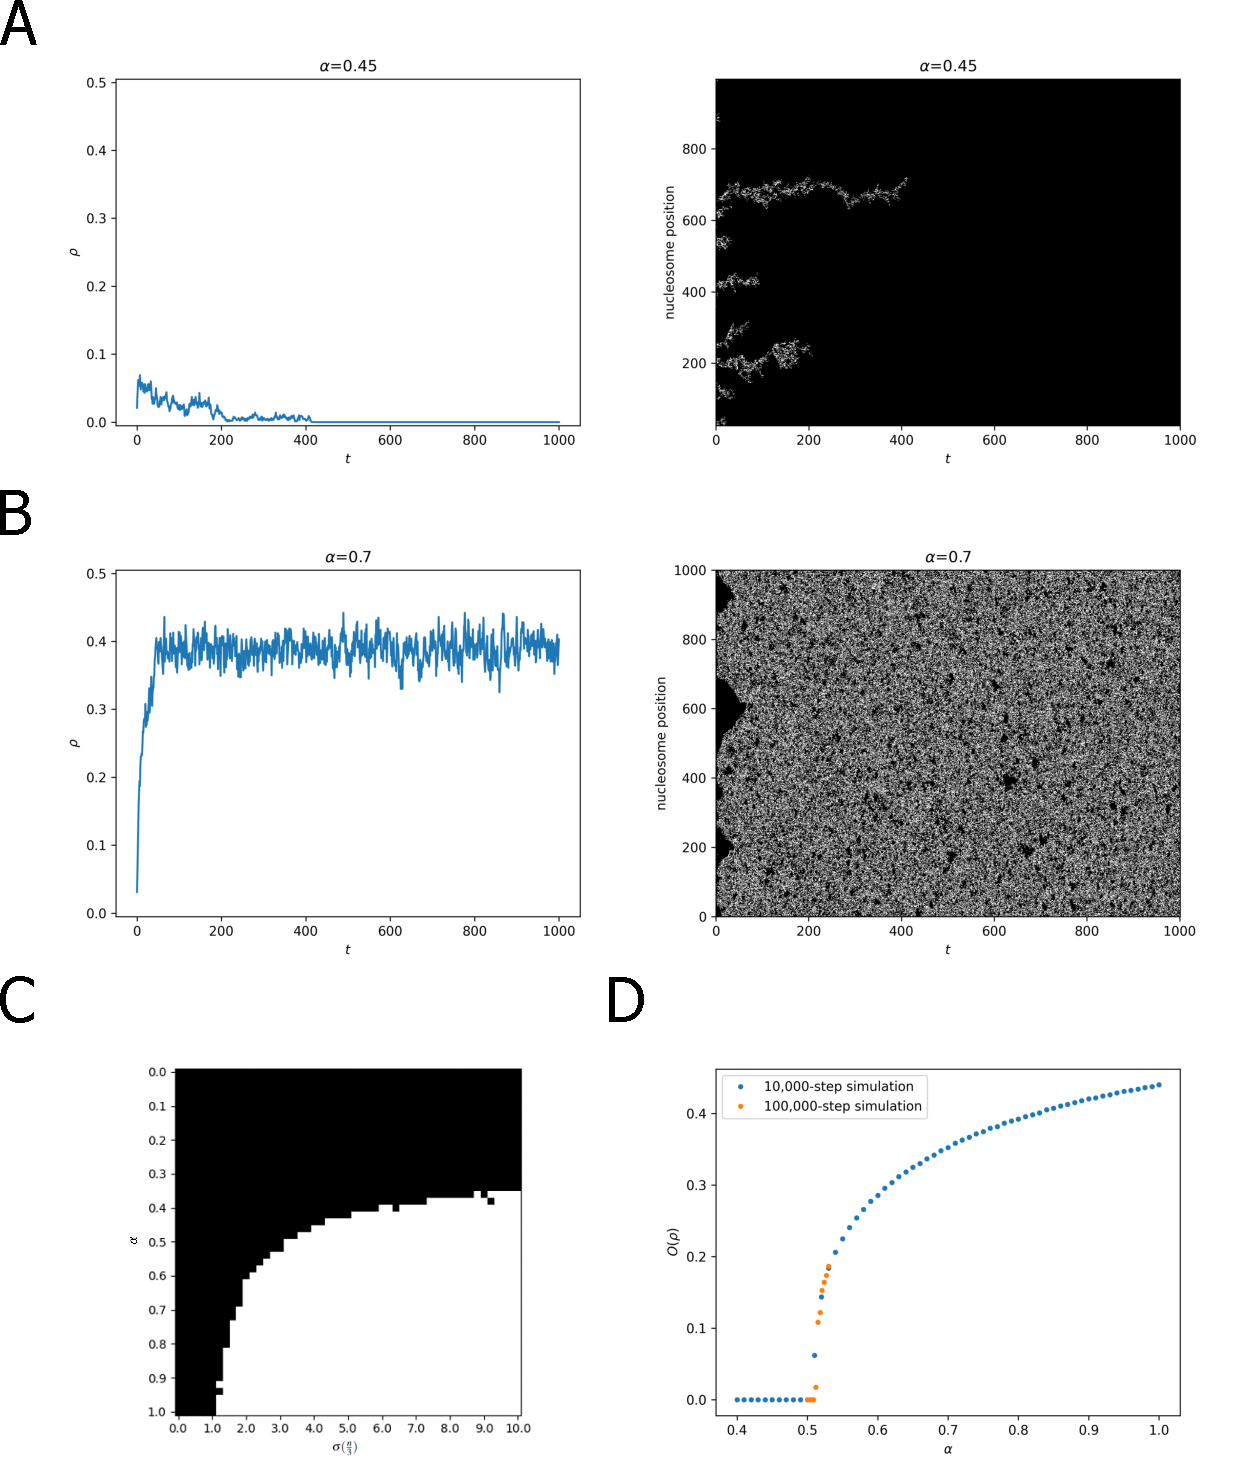
\includegraphics[width=0.9\textwidth]{chapter2/figures/model_behaviour.pdf}
  \caption[Typical behaviours of the basic model.]{Typical behaviours of the basic model. The simulations were conducted at $NN$=1000, $\rho_{0}$=0.02, $\sigma$=3, $rr$=3 if not otherwise stated. (A) The density evolution map and spatial pattern kymographs of a representative ‘dead’ behaviour ($\alpha$=0.45). (B) The density evolution map and spatial pattern kymographs of a representative ‘stabilised’ behaviour ($\alpha$=0.7). (C) Phase diagram of the model behaviour as a function of $\alpha$ and $\sigma$. Black represents the ‘dead’ behaviour and white represents the ‘stabilised’ behaviour for a specific parameter set. (D) Asymptotic density as a function of $\alpha$. 10 simulations were run for 10,000 (blue) or 100,000 time steps (orange) and the average density of the last 2,000 time steps was plotted as the asymptotic density. }
  \label{fig:modelBehaviour}
\end{figure}

We further tested if other factors might change the behaviours of the basic model. Generally, different simulations with the same parameter set generated qualitatively similar results (Figure~\ref{fig:parameterTest}A), suggesting that stochasticity is not important in determining the model behaviour. The number of nucleosomes also had little effect on the asymptotic density, though the smaller number showed a higher noise (Figure~\ref{fig:parameterTest}B). The initial value matters if the system has more than one steady state. To test it, I simulated the model from various initial densities. However, they all approached the same asymptotic value eventually (Figure~\ref{fig:parameterTest}C), indicating the model is likely to possess only one steady state. Note that the curves of high initial density appeared to be non-smooth in the first time step. This is because, independent of the initial value, they were all reduced to 0.5 after the first time step due to saturation. 

\begin{figure}[htbp]
  \centering
  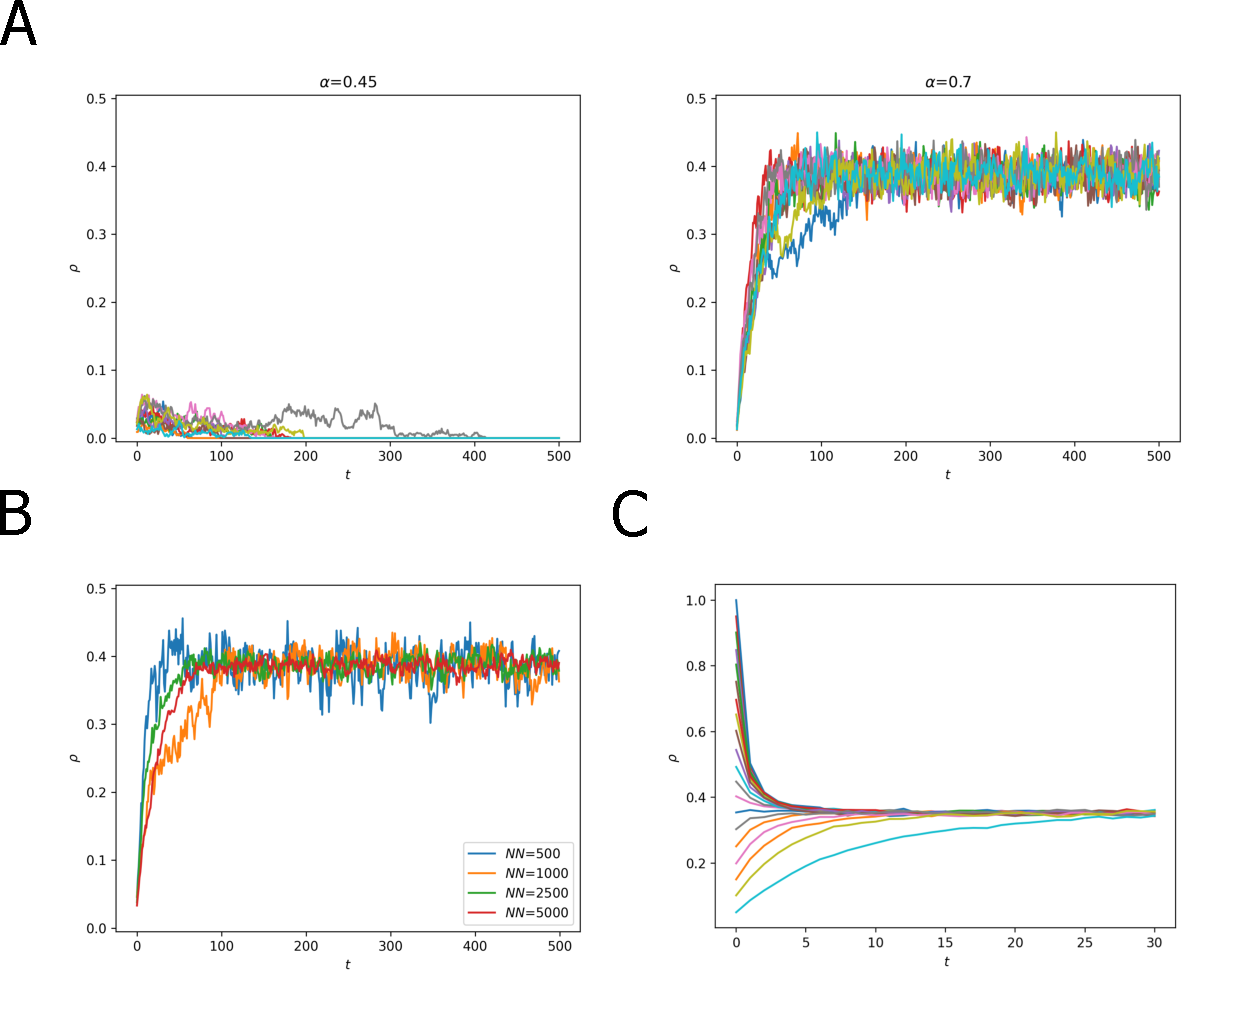
\includegraphics[width=0.9\textwidth]{chapter2/figures/parameter_test.pdf}
  \caption[The model behaviours are insensitive to stochasticity, nucleosome number and initial density.]{The model behaviours are insensitive to stochasticity, nucleosome number and initial density. The simulations were conducted at $NN$=1000, $\rho_{0}$=0.02, $\alpha$=0.7, $\sigma$=3, $rr$=3 if not otherwise stated. (A) The density evolution maps of different simulations of the representative ‘dead’ or 'stabilised' behaviour. 10 simulations were conducted for each behaviour, shown in different colours. (B) The density evolution map of the representative ‘stabilised' behaviour with different $NN$s. (C) The density evolution map of the representative ‘stabilised' behaviour with different $\rho_{0}$s. For each $\rho_{0}$, 100 simulations with $NN$=200 were conducted for 30 time steps. Each colour represents the average of 100 simulations. }
  \label{fig:parameterTest}
\end{figure}

In summary, the basic model (Figure~\ref{fig:basicmodelschematics}A) has two possible outcomes, with either all CENP-A nucleosomes being eventually lost or the density being maintained at a value much higher than that of the real biological systems. Moreover, in the second case, CENP-A nucleosome distribution is obviously different from the ‘islands’ pattern seen in extended chromatin experiments. Hence, we concluded that local deposition only is not sufficient to recapitulate the CENP-A dynamics \textit{in vivo}.

\subsection{Mean-field approximation is able to qualitatively explain the simulation results}

By simulating the old model and analyzing the results, we had a qualitative view of the basic model. To analyze the model
quantitatively, I wanted to apply analytical methods. Given the similarity between our model to CA, I chose mean-field
approximation as suggested by \citep{Sayama2013IntroductionSystems}. Instead of specific states of the system, mean-field approximation re-describes the dynamics of the system as how individual cells interact with the ’average state’ and how the ’average state’ itself changes over time. 

As mentioned above, the CENP-A nucleosome was expressed as cell state 1 whereas the H3 nucleosome was expressed as cell state 0 for the convenience of calculation. After applying mean-field approximation, the system now only has one state variable $\rho_{t}$, the density of 1s at time step t. To monitor its evolution, one needs to enumerate all possible scenarios of individual CA cells interacting with $\rho_{t}$ and their probabilities (Table~\ref{tab:MFAscenariosBasic}). Here, I started with one round of replenishment for simplicity. I identified 4 possible scenarios:

\begin{table}[htbp]
\centering
\caption{Possible scenarios of an individual cell in a one-round replenishment event}
\label{tab:MFAscenariosBasic}
\begin{tabular}{cccc}
\hline
\textbf{Scenario} & \textbf{Current state} & \textbf{Updated state} & \textbf{Probability} \\ \hline
(1) & 1                        & 0                      & 0                    \\
(2) & 1                        & 1                      & $\rho_{t}$                    \\
(3) & 0                        & 1                      & $(1 - \rho_{t})P_{0\rightarrow 1}(\rho_{t})$     \\
(4) & 0                        & 0                      & $(1 - \rho_{t})(1 - P_{0\rightarrow 1}(\rho_{t}))$ \\ \hline
\end{tabular}
\end{table}


(1) The cell state is 1 at time step t and will become 0 at time step t+1. The probability of finding a cell of 1 is simply $\rho_{t}$. But due to the assumption that CENP-A nucleosomes are not removed from the chromatin other than during dilution, the probability of this scenario is $\rho_{t} \times 0 = 0$. 

(2) The cell state is 1 at time step t and will stay 1 at time step t+1. For the same reason as above, the probability of this scenario is $\rho_{t} \times 1 = \rho_{t}$. 

(3) The cell state is 0 at time step t and will become 1 at time step t+1. Since the binary nature of cell state, the probability of finding a cell of 0 is $1 - \rho_{t}$. Then for this scenario to happen, one needs to consider the 0 to 1 state-transition function at $\rho_{t}$, which was denoted as $P_{0\rightarrow 1}(\rho_{t})$. Therefore, the probability of this scenario can be expressed as $(1 - \rho_{t})P_{0\rightarrow 1}(\rho_{t})$. 

(4) The cell state is 0 at time step t and will stay 0 at time step t+1. The occurrence of this scenario is equivalent to 
the fact that scenario (3) does not happen. Hence the probability of this scenario can be expressed as $(1 - \rho_{t})(1 - P_{0\rightarrow 1}(\rho_{t}))$.


After one round of replenishment, the density 1s equals the sum of the updated state of each scenario weighted by its respective probability. Hence, the one-round replenish function R can be written as:
\begin{equation}\label{eq:1}
\begin{split}
                R(\rho_{t})
                &= 0 \times 0 + 1 \times \rho_{t} + 1 \times (1 - \rho_{t})P_{0\rightarrow 1}(\rho_{t}) \\
                & + 0 \times (1 - \rho_{t})(1 - P_{0\rightarrow 1}(\rho_{t})) \\
                &=\rho_{t} + (1 - \rho_{t})P_{0\rightarrow 1}(\rho_{t})
\end{split}
\end{equation}
With the consideration that there is always a cell of 0 in the middle (position 0), the 0 to 1 state-transition function at $\rho_{t}$, $P_{0\rightarrow 1}(\rho_{t})$, can be calculated as follows: 
\begin{equation}\label{eq:2}
\begin{split}
                P_{0\rightarrow 1}(\rho_{t})
                &=\alpha(\rho_{t}f(-n)+\rho_{t}f(-n+1)\\
                &\quad+\ldots+0\cdot f(0)+\ldots+\\
                &\quad \rho_{t}f(n-1)+\rho_{t}f(n))\\
                &=\alpha(1-f(0))\rho_{t}
\end{split}
\end{equation}
Substitute $P_{0\rightarrow 1}(\rho_{t})$ in Equation~\ref{eq:1} with Equation~\ref{eq:2}, one can obtain:
\begin{equation}\label{eq:3}
                R(\rho_{t}) = \rho_{t} + (1 - \rho_{t})\alpha(1 - f(0))\rho_{t}
\end{equation}
By defining a new parameter $\omega = \alpha(1 - f(0))$, Equation~\ref{eq:3} becomes:
\begin{equation}\label{eq:4}
                R(\rho_{t}) = -\omega \rho_{t}^{2} + (1 + \omega) \rho_{t}
\end{equation}
The density of 1 at the next time step t+1 can then be calculated by implementing multiple rounds of replenishment as the recursion of function R and dilution as a halving of density:
\begin{equation}\label{eq:5}
                \rho_{t+1} = \frac{R^{rr}(\rho_{t})}{2}
\end{equation}
Combining Equation~\ref{eq:4} and Equation~\ref{eq:5}, the mean-field approximation of the basic model can be expressed as:
\begin{equation}\label{eq:6}
\begin{split}
            &\rho_{t+1} = \frac{R^{rr}(\rho_{t})}{2} \\
            &R(\rho_{t}) = -\omega \rho_{t}^{2} + (1 + \omega) \rho_{t}
\end{split}
\end{equation}
where $\omega = \alpha(1 - f(0))$. 

With the mathematical formulation of the basic model, we were able to analyse how the model behaviour was determined. To identify the existence of steady states and understand their changes according to $\alpha$, I started with the iterative map, or Cobweb plot, of the mean-field approximation with $\alpha$ ranging from 0 to 1 (Figure~\ref{fig:meanFieldApproximation}A). The Cobweb plot showed $\rho_{t+1}$ as a function of $\rho_{t}$. Its intersections with $y=x$ were therefore the fixed points of the model. Their stability can be assessed by the first-order derivative $y'$ at that point. If $\lvert y' \rvert \le 1$, the fixed point is stable. As shown in the Cobweb plot, the system’s fixed point(s) depends on $\alpha$. Low $\alpha$ has only one stable fixed point at $\rho_{t}$=0 while it becomes unstable for higher $\alpha$. Meanwhile, a non-zero stable fixed point starts to appear. To systematically study the effect of $\alpha$ on the steady state(s) of the system, I constructed the bifurcation diagram, where the fixed densities were plotted as a function of $\alpha$ (Figure~\ref{fig:meanFieldApproximation}B). The bifurcation diagram indicated that the fixed density stayed at 0 and did not change with $\alpha$ at the beginning. However, after around $\alpha$=0.3, the fixed density started to become positively correlated to $\alpha$. In mathematical terminology, the system undergoes saddle-node bifurcation as $\alpha$ increases. Interestingly, contrary to the simulation results that the asymptotic density is either 0 or a much higher value, the non-zero stable fixed point by the mean-field approximation can be very close to 0. We reasoned that it might be because the systems with small fixed densities were prone to stochasticity that could lead to 0 density and they would stay at 0 once reached there. Thus, in simulations, small fixed densities were unable to be observed. Next, I wanted to compare the predicted fixed densities by mean-field approximation with the asymptotic densities from the simulations. As shown in Figure~\ref{fig:meanFieldApproximation}C, the prediction showed a similar trend as the simulation data, albeit there were quantitative differences. Therefore, I concluded that mean-field approximation is capable of qualitatively describing the system. 

\begin{figure}[htbp]
  \centering
  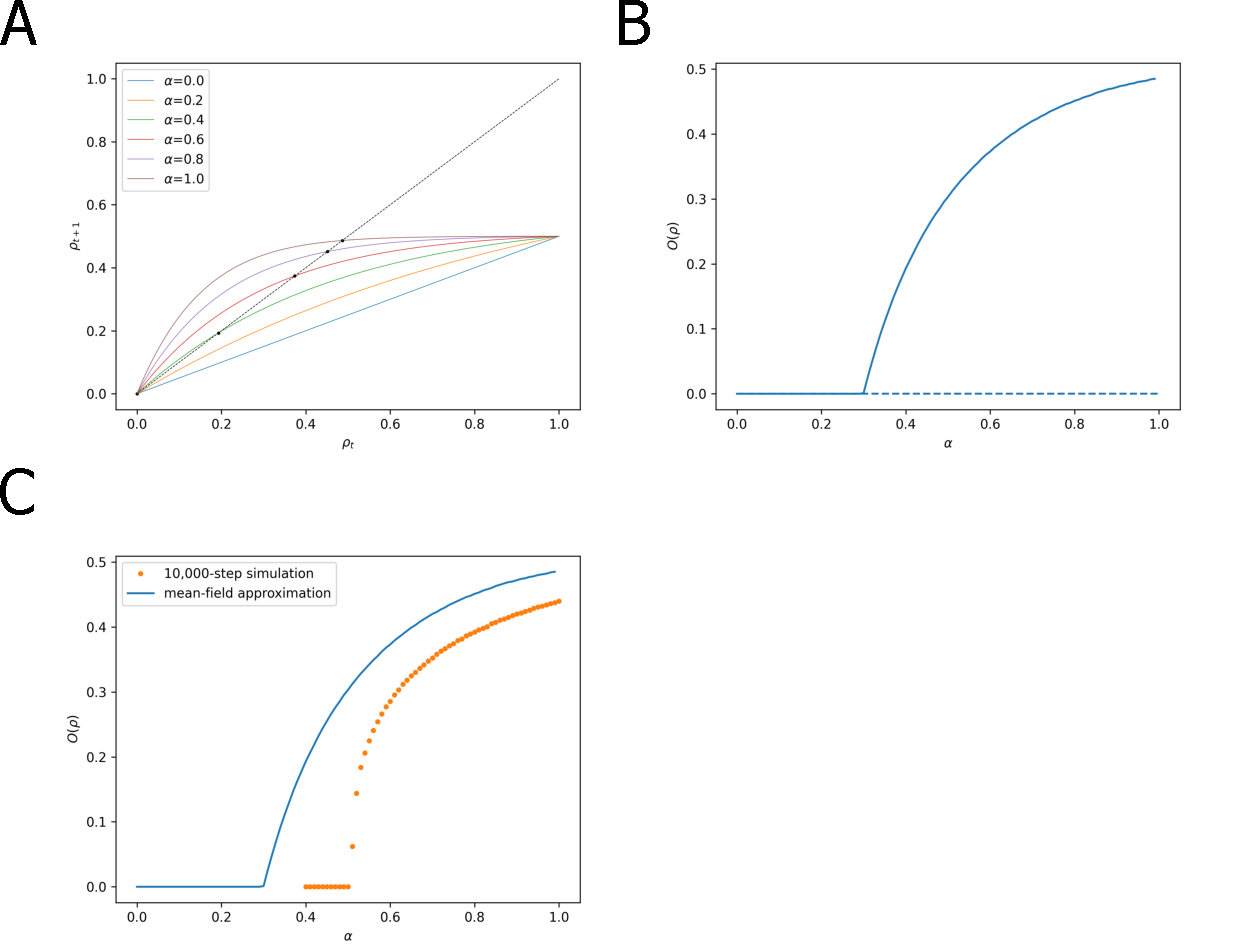
\includegraphics[width=0.9\textwidth]{chapter2/figures/mean-field_approximation.pdf}
  \caption[Mean-field approximation of the basic model]{Mean-field approximation of the basic model. $rr$=3 was used if not otherwise stated. (A) Cobweb plot of the basic model. The mean-field approximations of the basic model with different $\alpha$s were shown as coloured curves. Their intersections with $y = x$ represent fixed points, which were indicated as black dots. (B) Bifurcation diagram of the basic model. The fixed densities were plotted as a function of $\alpha$. The stable branch was shown as the solid line where as the unstable one was shown as the dotted line. (C) Comparison between the prediction of mean-field approximation and the simulation. The asymptotic densities were plotted as a function of $\alpha$. The stable branch of mean-field approximation was shown as the blue curve. The 10,000-step simulations were shown as orange dots.}
  \label{fig:meanFieldApproximation}
\end{figure}

\subsection{Global cooperative deposition generates bi-stability but cannot maintain the higher steady state at a low density}

As both behaviours of the basic model could not recapitulate CENP-A dynamics in real biological systems, we decided to introduce new mechanisms to the system. 

\begin{table}[htbp]
\centering
\caption{Possible scenarios of an individual cell in a one-round replenishment event}
\label{tab:MFAscenariosCoop}
\begin{tabular}{cccc}
\hline
\textbf{Scenario} & \textbf{Current state} & \textbf{Updated state} & \textbf{Probability} \\ \hline
(1) & 1                        & 0                      & 0                    \\
(2) & 1                        & 1                      & $\rho_{t}$                    \\
(3) & 0                        & 1                      & $(1 - \rho_{t})\rho_{t}P_{0\rightarrow 1}(\rho_{t})$     \\
(4) & 0                        & 0                      & $(1 - \rho_{t})(1 - \rho_{t}P_{0\rightarrow 1}(\rho_{t}))$ \\ \hline
\end{tabular}
\end{table}

\begin{equation}\label{eq:7}
\begin{split}
            &\rho_{t+1} = \frac{R^{rr}(\rho_{t})}{2} \\
            &R(\rho_{t}) = -\omega \rho_{t}^{3} + \omega \rho_{t}^{2} + \rho_{t}
\end{split}
\end{equation}
where $\omega = \alpha(1 - f(0))$. 

\subsection{Arbitrary number control leads to the formation of few CENP-A clusters}
\subsection{Spontaneous conversion can recapitulate the island pattern but not bi-stability}

\begin{table}[htbp]
\centering
\caption{The additional parameter(s) of the spontaneous conversion model}
\label{tab:parametersSpontaneousConversion}
\begin{tabular}{cl}
\hline
\textbf{Parameters} & \multicolumn{1}{c}{\textbf{Description}} \\ \hline
$\eta$                  & The rate of spontaneous conversion      \\ \hline
\end{tabular}
\end{table}

\begin{equation}\label{eq:8}
\begin{split}
            &\rho_{t+1} = \frac{R^{rr}(\rho_{t})}{2} + \eta \\
            &R(\rho_{t}) = -\omega \rho_{t}^{2} + (1 + \omega) \rho_{t}
\end{split}
\end{equation}
where $\omega = \alpha(1 - f(0))$. 
\section{Discussion}

% \chapter{Investigating the Molecular Mechanisms of Tension-dependent Re-localisation of Shugoshin}

\section{Introduction}
Centromere executes its function of coordinating chromosome segregation partially by controlling the subcellular location of critical regulators. A remarkable example is the tension-dependent re-localisation of shugoshin. 

To be segregated into different daughter cells later, sister chromatids need to be bipolarly attached to the spindle in mitosis or meiosis II, which is called bi-orientation \citep{Tanaka2010Kinetochore-microtubuleBi-orientation}. Bi-oriented sister chromatids come under tension due to the counteraction between the resistance of cohesion and the pulling of microtubules. Cells sense a lack of tension and destabilise erroneous microtubule-kinetochore attachment, a process termed error correction, meanwhile delaying cell cycle progression until tension is generated \citep{Nicklas1997HowChromosomes, Nicklas1994, Tanaka2010Kinetochore-microtubuleBi-orientation}. The conserved shugoshin protein family is important for the establishment of tension \citep{Watanabe2005, Clift2011, Gutierrez-Caballero2012Shugoshins:Centromere, Marston2015, Zhang2020FunctioningMitosis}. The name itself, 'guardian spirit' in Japanese, comes from its well-conserved canonical function of cohesion protection in meiosis I \citep{Lister2010Age-relatedSgo2, Llano2008Shugoshin-2Mice, Lee2008, Rattani2013Sgol2Oocytes, Marston2004a, Kitajima2004a, Katis2004, Rabitsch2004TwoII, Kerrebrock1992TheDifferentiation, Cromer2013CentromericInterkinesis, Zamariola2014SHUGOSHINsThaliana, Wang2011OsSGO1Meiosis, Hamant2005AFunctions, Ma2021MeikinI, Miyazaki2017HierarchicalI}. In vertebrates, shugoshin also protects centromeric cohesion from Wapl-mediated cohesin removal pathway in mitosis \citep{Rivera2009ShugoshinExtracts, Shintomi2009ReleasingSgo1, Huang2007, Tang2006a, McGuinness2005ShugoshinCells, Kitajima2005, Salic2004VertebrateMitosis, Liang2019ACells}. Shugoshin further assists cohesion protection by directly sequestering separase with the SAC component Mad2 \citep{Rattani2013Sgol2Oocytes, Hellmuth2020Securin-independentShugoshinMAD2, Orth2011ShugoshinMad2}. Apart from cohesion protection, shugoshin additionally promotes bi-orientation by facilitating error correction \citep{Meppelink2015Shugoshin-1Bi-orientation, Huang2007, Peplowska2014, Nerusheva2014, Verzijlbergen2014, Tsukahara2010a, Yamagishi2010, Hadders2020UntanglingMitosis, Broad2020AuroraCells, Kawashima2007, Vanoosthuyse2007, Rivera2012} and, at least in yeast, contributing to the geometry of the centromeric region biased towards a shape where sister kinetochores are more easily captured by microtubules from the opposite spindle poles \citep{Indjeian2007, Haase2012Bub1Dynamics, Verzijlbergen2014, Peplowska2014, Sane2021ShugoshinDisassembly}. Despite different molecular details in various species, all these functions are implemented by shugoshin acting as an adaptor recruiting different effector proteins to the centromeric region, including PP2A-B' \citep{Xu2009StructureInteraction, Ueki2021AMitosis}, CPC \citep{Abad2022MechanisticCPC}, MCAK \citep{Tanno2010} and condensin \citep{Verzijlbergen2014, Yahya2020}. 

Interestingly, the location of shugoshin has been found to change in response to tension across species. Human Sgo1 and Sgo2 redistribute from the inner centromere towards the kinetochore upon tension establishment in mitosis \citep{Huang2007, Lee2008, Liu2013, Asai2020}. Mouse Sgo2 follows the same pattern in meiosis II \citep{Lee2008, Gomez2007}. In budding yeast, tension removes its only shugoshin protein Sgo1 from peri-centromere \citep{Eshleman2014, Nerusheva2014, Paldi2020ConvergentPericentromeres}. Although the effect of tension has not been directly studied, locations are different between metaphase and anaphase for \textit{Drosophila} MEI-S332 (mitosis and meiosis II) and fission yeast Sgo2 (mitosis) \citep{Clarke2005, Kawashima2007}, raising the possibility that they also undergo tension-dependent re-localisation. 

Re-localisation of shugoshin is functionally relevant. It has been proposed as key to tension sensing \citep{Marston2015}. Screening in budding yeast identified Sgo1 being required to delay anaphase onset in the absence of tension \citep{Indjeian2005a}. Later, it was shown to be due to its role in preventing SAC silencing \citep{Jin2013TheAttachment}. Given the function of Sgo1 to support CPC localisation, it was reasoned that tension-dependent re-localisation of Sgo1 triggers the removal of CPC from the centromere, leading to SAC silencing \citep{Nerusheva2014}. In support of this model, artificially tethering Sgo1 to the kinetochore caused prolonged metaphase \citep{Su2021SumoylationAnaphase}. In mammals, the re-localisation is thought to inactivate cohesin protection \citep{Lee2008}. Indeed, impaired human Sgo1 re-localisation increased lagging chromosomes in anaphase \citep{Liu2013}. Besides, at least in budding yeast, the re-localisation of shugoshin might be the signal for chromosome condensation. The key condensation player condensin spreads from the centromere to chromosome arms in a tension-dependent manner \citep{Leonard2015}. As its interactor with a similar response to tension, Sgo1 potentially mediates the spread. Consistent with this idea, mitotic chromosome condensation is abolished in \textit{sgo1} mutant \citep{Kruitwagen2018}. 

It is well established across species that the SAC component Bub1 kinase at the kinetochore phosphorylates threonine 120 of histone H2A (serine 121 in yeast) around centromeric chromatin, providing a high-affinity marker for shugoshin \citep{Rivera2012, Boyarchuk2007Bub1Centromere, Williams2017Bub1Kinetochores, Kitajima2005, Perera2010, Tang2004, Fernius2007Bub1Mitosis, Kiburz2005, Kawashima2010a}. Nevertheless, the localisation of shugoshin is further regulated by complicated, not fully understood, interplay of various factors through reversible PTMs. In human cells, a step-wise recruitment model of Sgo1 has been proposed \citep{Liu2013, Liu2013a, Liu2015}. Sgo1 is first recruited proximal to the kinetochore due to direct binding to nucleosomes with H2A-pT120. Pol II-mediated centromeric transcription then disengages Sgo1 from nucleosomes, allowing it to reach the inner centromere. Finally, Sgo1 phosphorylated at threonine 346 by CDK is captured by cohesin there. A number of other factors supporting shugoshin localisation have been reported in different species, including HP1 \citep{Yamagishi2008, Kang2011, Perera2010}, CPC \citep{Huang2007, Tanno2010, Rivera2012, Kawashima2007, Boyarchuk2007Bub1Centromere, Resnick2006INCENPDrosophila}, PP2A \citep{Tang2006a}, CENP-A \citep{Petty2018ConnectingCheckpoint, Eot-Houllier2018AuroraFatigue, Mishra2018BuddingChromatin} and H3 \citep{Buehl2018a, Luo2016}, while Polo kinase \citep{Clarke2005}, SET \citep{Qu2019SETSegregation, Krishnan2017Phospho-H1Mitosis}, KAT2A \citep{Petty2018ConnectingCheckpoint} and PP2A \citep{Nerusheva2014} were suggested to de-localise it. 

The mechanism of shugoshin tension-dependent re-localisation is less well understood. \cite{Nerusheva2014} attempted to address it in budding yeast, yet questions are left to be answered. It was proposed that reduced Bub1 activity at peri-centromere by tension leads to the de-phosphorylation of its substrate(s), thus resulting in the removal of Sgo1 (Figure~\ref{fig:naive}). How Bub1 activity in a particular area is regulated by tension remains to be elucidated. Due to technical difficulties, it was unable to directly monitor H2A-pS121 by that time, leaving the effect of tension on it untested. Moreover, this model predicts the existence of at least one phosphatase antagonizing Bub1. Although it was found that PP2A-B' (Rts1 in budding yeast) negatively regulates Sgo1 enrichment at the peri-centromere, whether it is responsible for Sgo1 de-localisation is unclear. The human model emphasizes phospho-regulation of shugoshin interaction with cohesin by tension underlying its movement from the inner centromere to the kinetochore-proximal region \citep{Liu2013, Liu2015}. It is interesting to explore if this mechanism could be conserved in budding yeast as well. Besides, the exact localisation of human H2A-pT120 by IF is inconsistent in the literature, with reports arguing it covers both the inner centromere \citep{Yamagishi2010} and the kinetochore proximity or it is usually only at the latter \citep{Liu2013}. Due to the repetitive nature of human centromere, the two arguments could not be distinguished by sequence-based technology such as ChIP. Whereas budding yeast can be used to address this question for its point centromere structure. 

\begin{figure}[htbp]
  \centering
  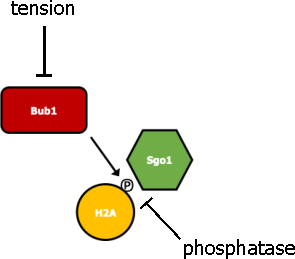
\includegraphics[width=0.3\textwidth]{figures/naive model.pdf}
  \caption[Proposed budding yeast model of tension-dependent re-localisation of Sgo1]{Proposed budding yeast model of tension-dependent re-localisation of Sgo1. Tension causes a reduction of Bub1 phosphorylation capability at peri-centromere, resulting in the de-phosphorylation of the substrates (H2A-S121 is used as an example here) by the counteracting phosphatase. Sgo1 is therefore de-localised from the peri-centromere.}
  \label{fig:naive}
\end{figure} 

\nomenclature{SAC}{Spindle Assembly Checkpoint}
\nomenclature{CPC}{Chromosome Passenger Complex}
\nomenclature{PP2A}{Protein Phosphatase 2A}
\nomenclature{MCAK}{Mitotic Centromere-Associated Kinesin}
\nomenclature{SET}{SET nuclear proto-oncogene}
\nomenclature{CDK}{Cyclin-Dependent Kinase}
\nomenclature{Pol II}{RNA Polymerase II}
\nomenclature{HP1}{Heterochromatin Protein 1}
\nomenclature{KAT2A}{lysine AcetylTransferase 2A}
\nomenclature{PTM}{Post Translational Modification}
\nomenclature{ChIP}{Chromatin ImmunoPrecipitation}
\nomenclature{IF}{ImmunoFluorescence}


\section{Results}
\subsection{Whether tension pulls Bub1 away from the peri-centromere border is inconclusive}
It is unclear how tension inhibits Bub1 activity at the peri-centromere. One possibility is that kinetochore-localised Bub1 is pulled away from its substrates at the peri-centromere because of tension \citep{Nerusheva2014}. This hypothesis is further supported by the study on peri-centromeric chromatin conformation showing that tension reduces the interaction between the core centromere and peri-centromeric borders \citep{Paldi2020ConvergentPericentromeres}, where Sgo1 mainly localises revealed by ChIP-seq \citep{Verzijlbergen2014, Deng2018}. 

To test this idea, I first wanted to measure FRET between Bub1 and nucleosomes. If the hypothesis is true, the FRET signal should decrease in the presence of tension. hence, I constructed a strain bearing \textit{BUB1-mNG HTB1-mCherry pMET-CDC20}. To validate the method, cells were synchronized in G1 and released into a metaphase arrest without tension by nocodazole, as this condition is expected to give a higher FRET signal. Unfortunately, it was unable to detect any FRET signal between Bub1 and Htb1, leaving the method usable (Figure~\ref{fig:FRET}). The problem is possibly due to the low expression of Bub1 protein and the small size of budding yeast. 
\nomenclature{FRET}{Förster Resonance Energy Transfer}

\begin{figure}[htbp]
  \centering
  \includesvg[width=0.6\textwidth]{figures/Bub1-mNG Htb1-mCherry FRET.svg}
  \caption[Representative image of FRET between Bub1-mNG and Htb1-mCherry of metaphase cells without tension]{Representative image of FRET between Bub1-mNG and Htb1-mCherry of metaphase cells without tension. Bleed-through from both fluorophores to the FRET channel are subtracted. }
  \label{fig:FRET}
\end{figure} 

As an alternative approach, I decided to directly measure the distance between Bub1 and peri-centromeric borders, which is expected to increase by tension. To this end, I labelled one peri-centromeric border of chromosome I using the Tet-On system, with a tetO array on the locus and tetR-tdTomato under a constitutive promoter. Cells bearing \textit{BUB1-mNG pMET-CDC20} and the labelled peri-centromeric border of chromosome I were synchronized in G1 and released into methionine-containing media for a metaphase arrest with tension. Time-lapse live-cell imaging was performed since the G1 release. Bub1-mNG appears as one focus as cells enter the S phase, indicated by the appearance of small buds. This is due to centromere clustering in budding yeast \citep{Taddei2012StructureNucleus}. All kinetochores  are seen together as one dot under current light microscopes. Bub1-mNG then splits into two foci due to sister kinetochores separating by tension. On the other hand, tetR-tdTomato stays as one focus from the beginning of imaging. Occasionally, it splits into two foci after the separation of Bub1-mNG foci (Figure~\ref{fig:periCEN}A). The distance between Bub1-mNG and tetR-tdTomato focus $L$ was measured. After the separation of Bub1-mNG, there could be two $L$s in one cell. I arbitrarily named the shorter one as $L_{1}$ and the longer one as $L_{2}$. The inter-kinetochore distance measured from the distance between Bub1-mNG dots was used as the indicator of tension. Before Bub1-mNG separation, $L$ ranges from 0.01 to 1.19 \si{\micro\metre} with a median of 0.32 \si{\micro\metre}. After Bub1-mNG separation, $L_{1}$ and $L_{2}$ together gave a data set showing a slight increase, ranging from 0.01 to 1.24 \si{\micro\metre} with a median of 0.40 \si{\micro\metre}. However, if analysed individually, $L_{1}$ is not correlated with the inter-kinetochore distance ($R^2 = 0.03$) despite $L_{2}$ shows a moderated correlation ($R^2 = 0.59$) (Figure~\ref{fig:periCEN}B).This result suggests the distance between one of the Bub1-mNG foci and the peri-centromere border is independent of tension, arguing against the hypothesis of Bub1 being pulled further away from its substrates at the peri-centromere. Whereas the other Bub1-mNG focus does become further, favouring the hypothesis. Therefore, whether tension pulls Bub1 away from the peri-centromere border is inconclusive. 


\begin{figure}[htbp]
  \centering
  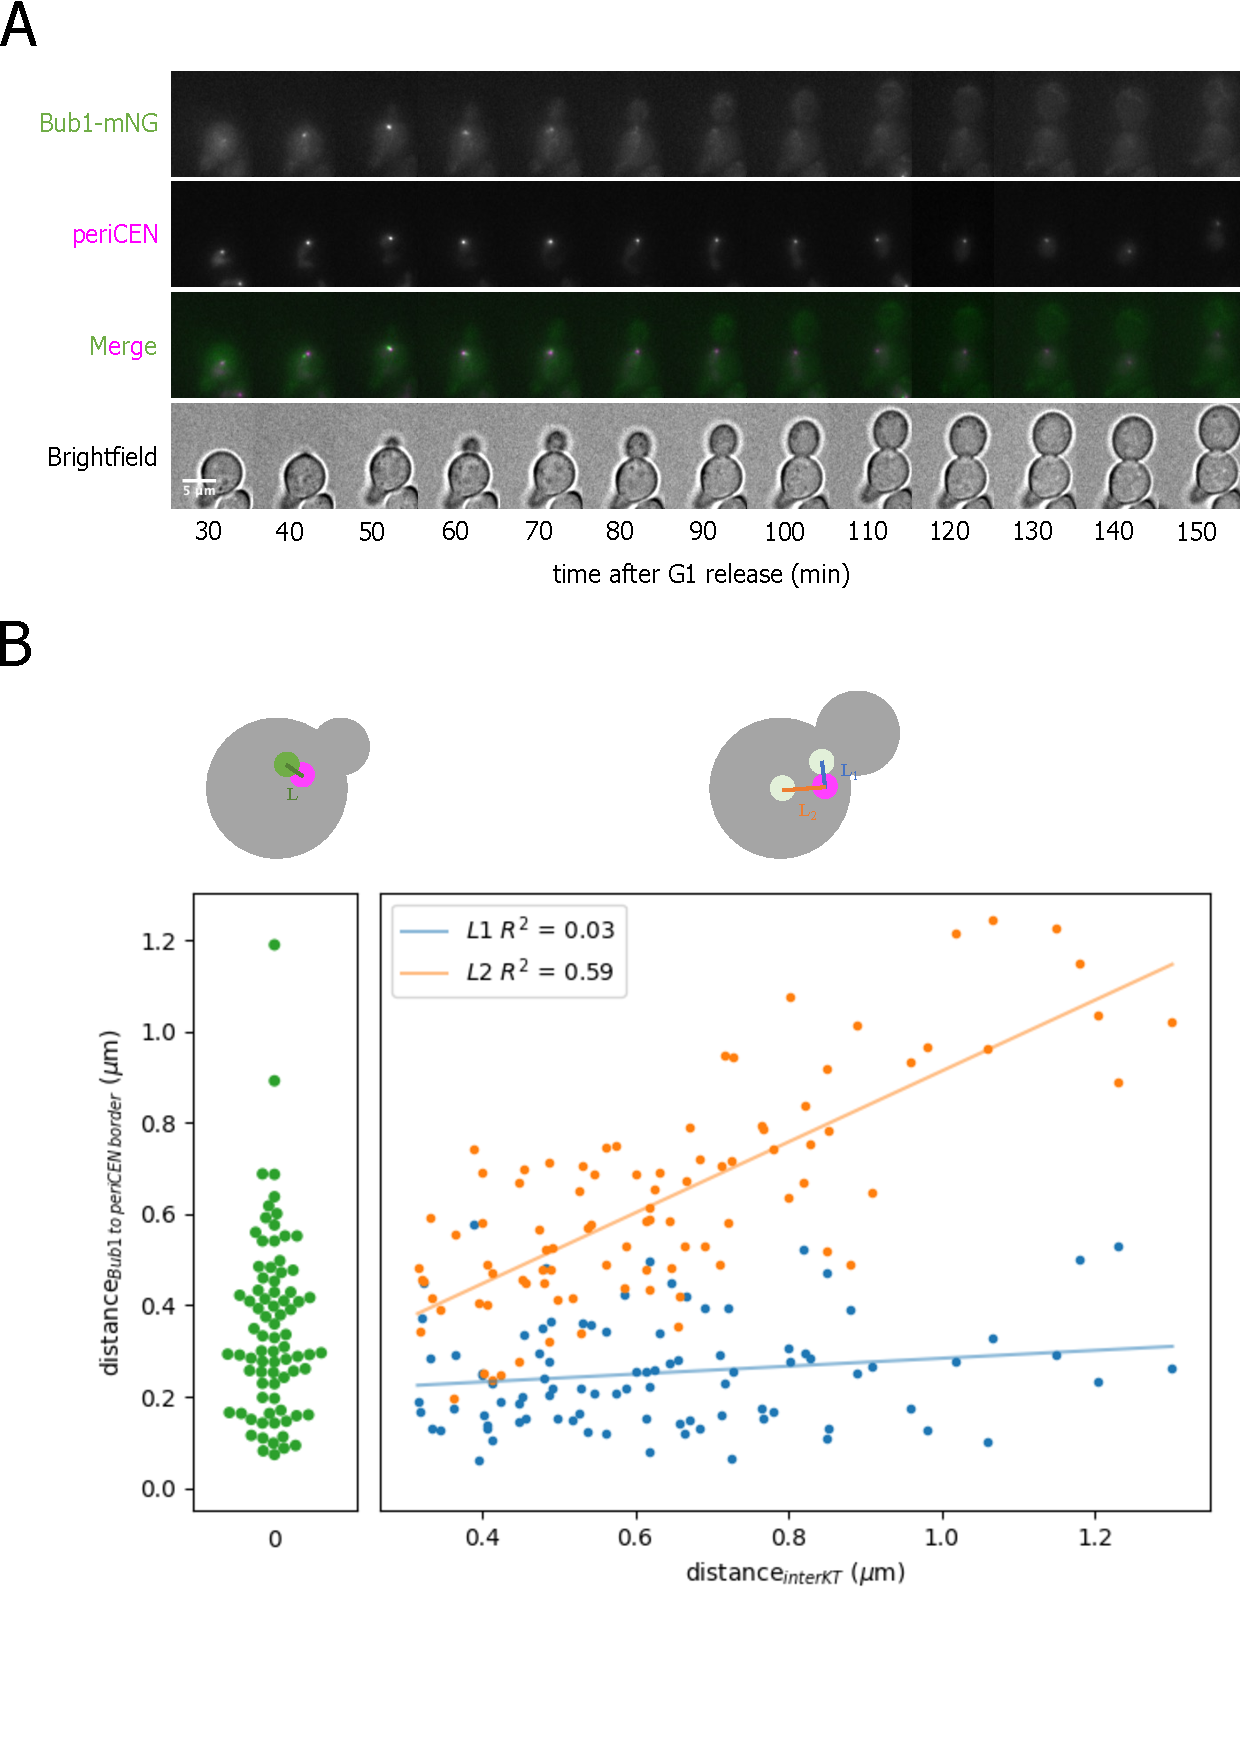
\includegraphics[width=0.9\textwidth]{figures/Bub1-mNG peri-cen.pdf}
  \caption[The shorter distance between Bub1 and peri-centromere is independent of the inter-kinetochore distance]{The shorter distance between Bub1 and peri-centromere is independent of the inter-kinetochore distance. (A) Montage of representative time-lapse imaging. (B) Scatter plot showing the relation of Bub1-to-peri-centromere distance and inter-kinetochore distance. N=30 cells were followed over time and quantified for $L$ (the distance before Bub1-mNG separation), $L_{1}$ (the shorter distance after Bub1-mNG separation) and $L_{2}$ (the longer distance after Bub1-mNG separation), which are presented in green, orange and blue, respectively. The line with the same colour represents the model of simple linear regression. }
  \label{fig:periCEN}
\end{figure} 

\nomenclature{mNG}{mNeonGreen}

\subsection{Bub1 is de-localised from the kinetochore by tension}
During data analysis of the previous experiment, I noticed a reduction in fluorescence intensity of Bub1-mNG foci as they separate to an extent that they are barely visible at the end of imaging. This cannot be simply explained by photo-bleaching because tdTomato is supposed to have a shorter bleaching time than mNG, yet it remains visible (Figure~\ref{fig:periCEN}A). The observation raises the possibility that the kinetochore localisation of Bub1 could be under the regulation of tension, leading to the physical separation from its substrates. The idea that Bub1 localisation could be regulated by tension has been implicated in literature \citep{Asai2020, Proudfoot2019, Jin2017PrematureCerevisiae}. To test this, I wanted to quantify the dynamics of the amount of Bub1 at the kinetochore as well as the inter-kinetochore distance. Since Bub1-mNG becomes indistinguishable from the background after separation, I chose to use the outer-kinetochore protein Mtw1 as a more reliable measure of the inter-kinetochore distance. I constructed a strain bearing \textit{BUB1-mNG MTW1-tdTomato pMET-CDC20}. Time-lapse live-cell imaging was again performed since the G1 release (Figure~\ref{fig:bub1mtw1}A). As expected, Bub1-mNG follows the same dynamics as in the previous experiment. While Mtw1-tdTomato appears as one focus at the start of imaging and then splits into two foci as the cell cycle progresses (Figure~\ref{fig:bub1mtw1}B). Further quantification showed that the fluorescence intensity of kinetochore Bub1-mNG peaks at 60 \si{\minute} since G1 release, with an over 2-fold decrease at 70 \si{\minute}, coinciding with the beginning of Mtw1-tdTomato foci separation (Figure~\ref{fig:bub1mtw1}C). This indicates that kinetochore-localised Bub1 is reduced upon the establishment of bi-orientation. 

\begin{figure}[htbp]
  \centering
  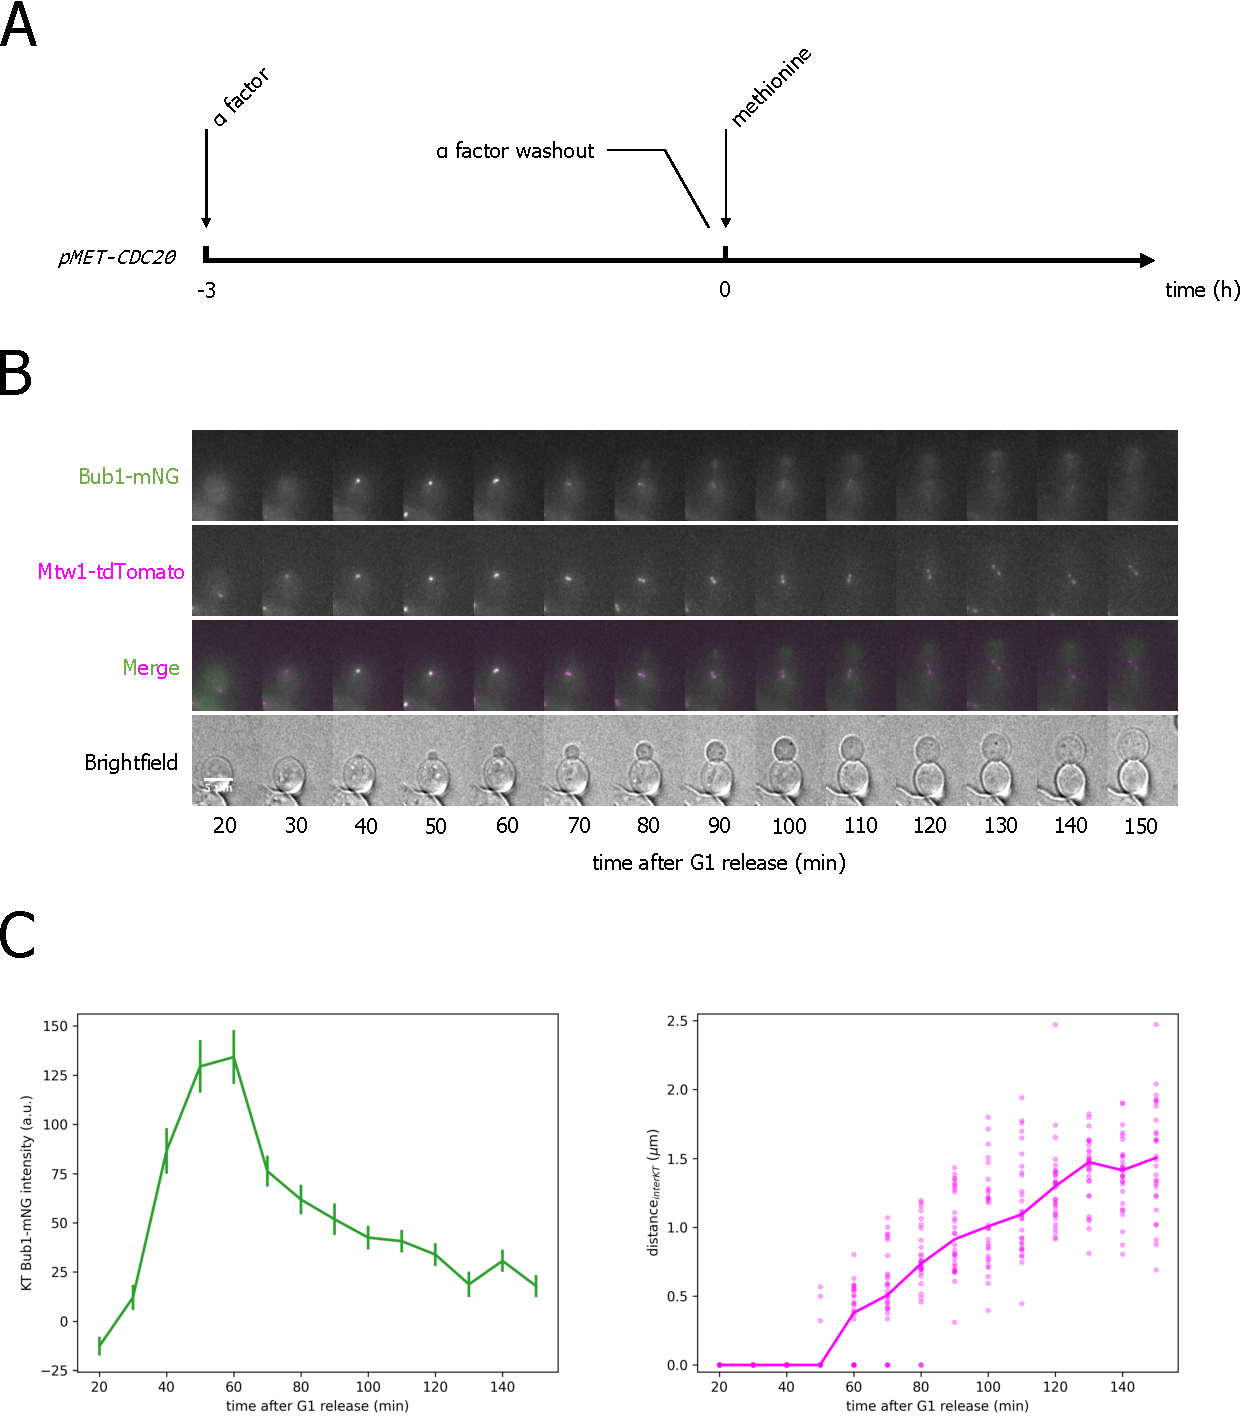
\includegraphics[width=0.9\textwidth]{figures/Bub1-mNG vs Mtw1-td.pdf}
  \caption[Kinetochore-localised Bub1 is reduced upon bi-orientation]{Kinetochore-localised Bub1 is reduced upon bi-orientation. (A) Schematics of experimental procedures. (B) Montage of representative time-lapse imaging. (C) N=30 cells were followed over time and quantified for kinetochore Bub1-mNG fluorescence intensity and inter-kinetochore distance. Left panel: mean fluorescence intensity of Bub1-mNG at the kinetochore as a function of time. The error bar represents the standard error. Right panel: Median inter-kinetochore distance as a function of time. Individual data points are shown as dots. }
  \label{fig:bub1mtw1}
\end{figure} 

I then sought to test whether the reduction in Bub1 kinetochore localisation is due to protein degradation or re-localisation. Human Bub1 is degraded by APC in anaphase \citep{Qi2007KEN-box-dependentComplex/cyclosome} but it is not known in budding yeast. Hence, I performed a synchronised mitotic time course experiment followed by western blotting to check Bub1 protein expression. Cells bearing \textit{BUB1-6HA} were synchronised in G1 and released into rich media. $\alpha$ factor was added 60 \si{\minute} after the release to arrest cells in the next G1 (Figure~\ref{fig:bub1timecourse}A). Tubulin IF was used to examine the progression of the cell cycle. At 75 \si{\minute} after G1 release, over 80\% of cells were in metaphase while most cells were in anaphase at 90 and 105 \si{\minute} (Figure~\ref{fig:bub1timecourse}B). Western blotting with anti-HA antibody showed Bub1 protein level reached its apex at 90 \si{\minute} and started to decrease since 105 \si{\minute} (Figure~\ref{fig:bub1timecourse}C), suggesting Bub1 is degraded in late anaphase in budding yeast. Therefore, protein degradation could not be the reason for reduced Bub1 kinetochore localisation in metaphase in the previous experiment. Interestingly, Bub1 experienced changes in electrophoretic mobility at the early stage of the cell cycle, indicating its phosphorylation status might be actively regulated. As this is beyond the scope of my project, this was not investigated further. 

\begin{figure}[htbp]
  \centering
  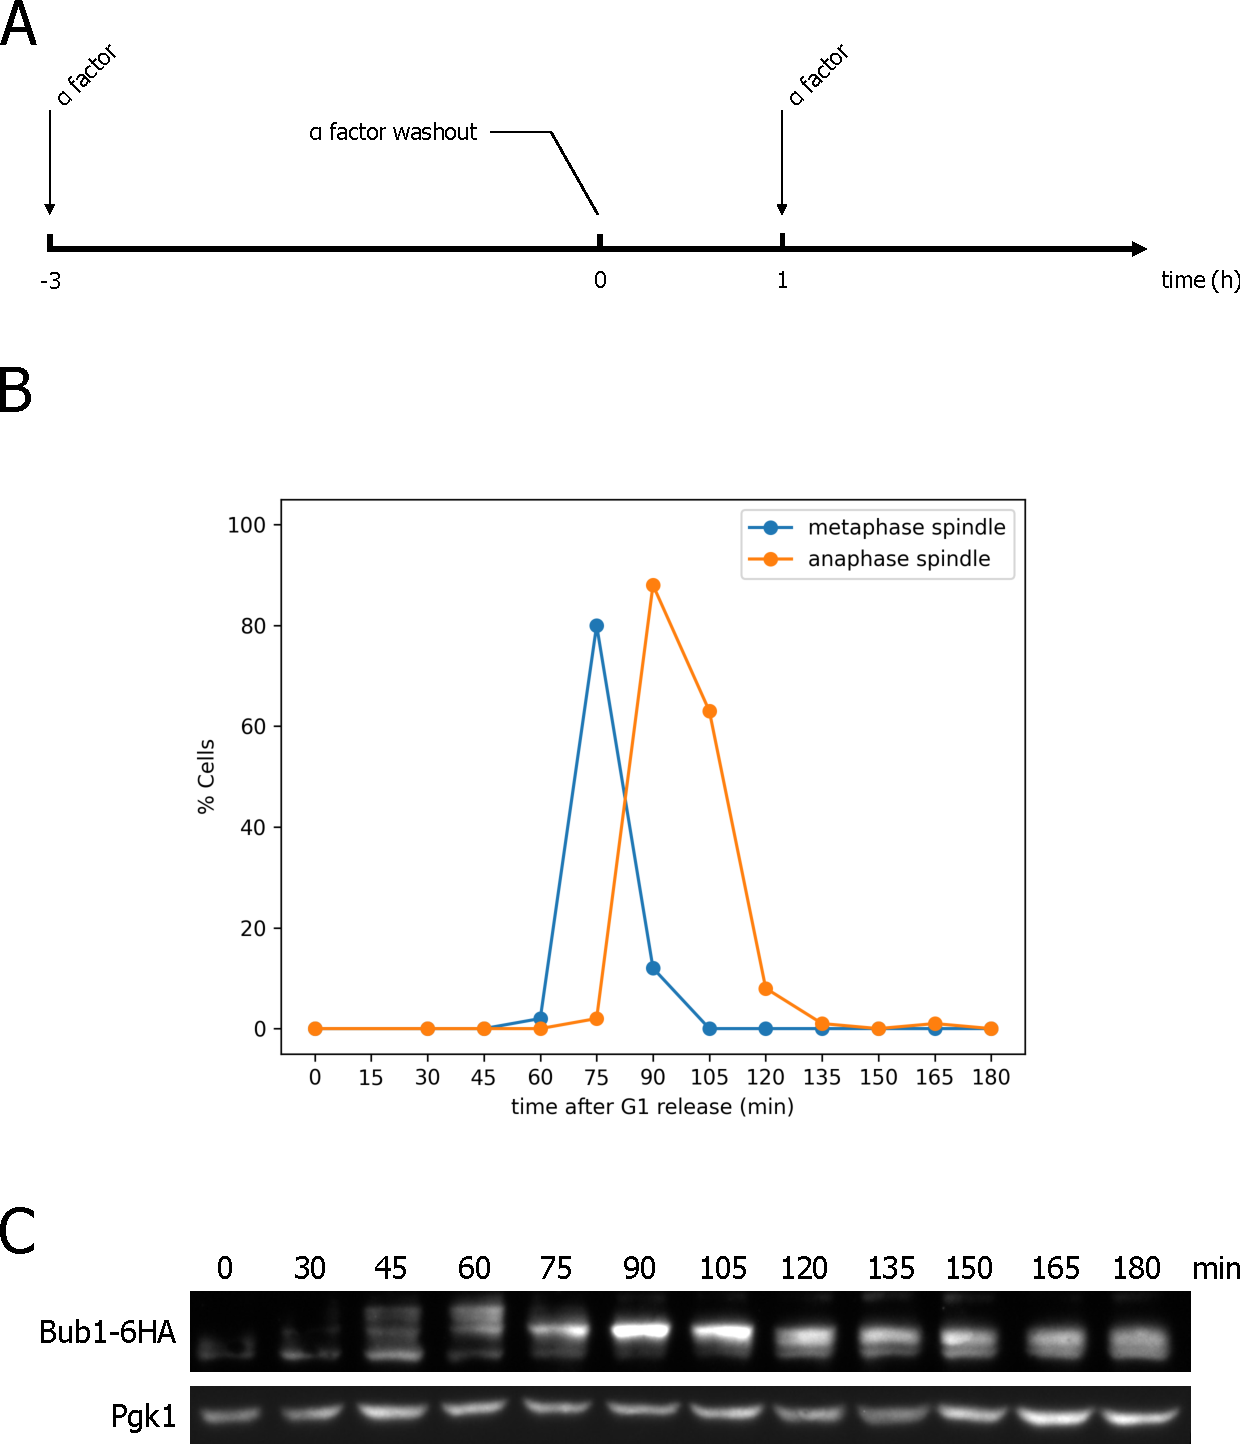
\includegraphics[width=0.9\textwidth]{chapter3/figures/Bub1-6HA time course.pdf}
  \caption[Bub1 is not degraded until anaphase]{Bub1 is not degraded until anaphase. (A) Schematics of experimental procedures. (B) The proportion of cells with metaphase or anaphase spindle over time by tubulin IF. (C) Western blotting with anti-HA antibody to detect Bub1 protein. Pgk1 was used as the loading control.}
  \label{fig:bub1timecourse}
\end{figure} 

The experiments above suggest that Bub1 is re-localised from the kinetochore upon bi-orientation. Given that both tension and kinetochore-microtubule attachment are established in this case, it is unkown whether tension is required for Bub1 de-localisation besides attachment. To abolish tension without disrupting attachment, I decided to disable sister chromatid cohesion by depleting the kleisin subunit Scc1 of the cohesin complex. Cells from Figure~\ref{fig:bub1mtw1} with or without additional \textit{pMET-SCC1} were synchronised in G1. Methionine was added 45 \si{\minute} before releasing to pre-clean Scc1 in the \textit{pMET-SCC1} strain. Live-cell imaging was performed to quantify kinetochore Bub1-mNG fluorescence intensity and inter-kinetochore distance (Figure~\ref{fig:bub1metscc1}A). As expected, the \textit{pMET-SCC1} strain exhibited increased inter-kinetochore distance ($\sim$2.5 \si{\micro\metre} towards the end of the experiment) compared to the wild type ($\sim$1.5 \si{\micro\metre} towards the end of the experiment), indicating a reduction in sister chromatid cohesion. Unlike the wild type, the signal of kinetochore Bub1-mNG is maintained at a similar value after 60 \si{\minute} from G1 release in the \textit{pMET-SCC1} strain (Figure~\ref{fig:bub1metscc1}B and C), suggesting Bub1 is not removed from the kinetochore in the absence of tension while no additional disruption was applied on attachment. To rule out the potential artefacts from \textit{pMET-SCC1} causing an increase in Bub1 expression, I used western blotting to check the Bub1 protein expression level in the wild type and the \textit{pMET-SCC1} strain arrested in metaphase by methionine depletion. No obvious difference was observed (Figure~\ref{fig:bub1metscc1}D). Hence, the kinetochore localisation of Bub1 is reduced by tension. 

\begin{figure}[htbp]
  \centering
  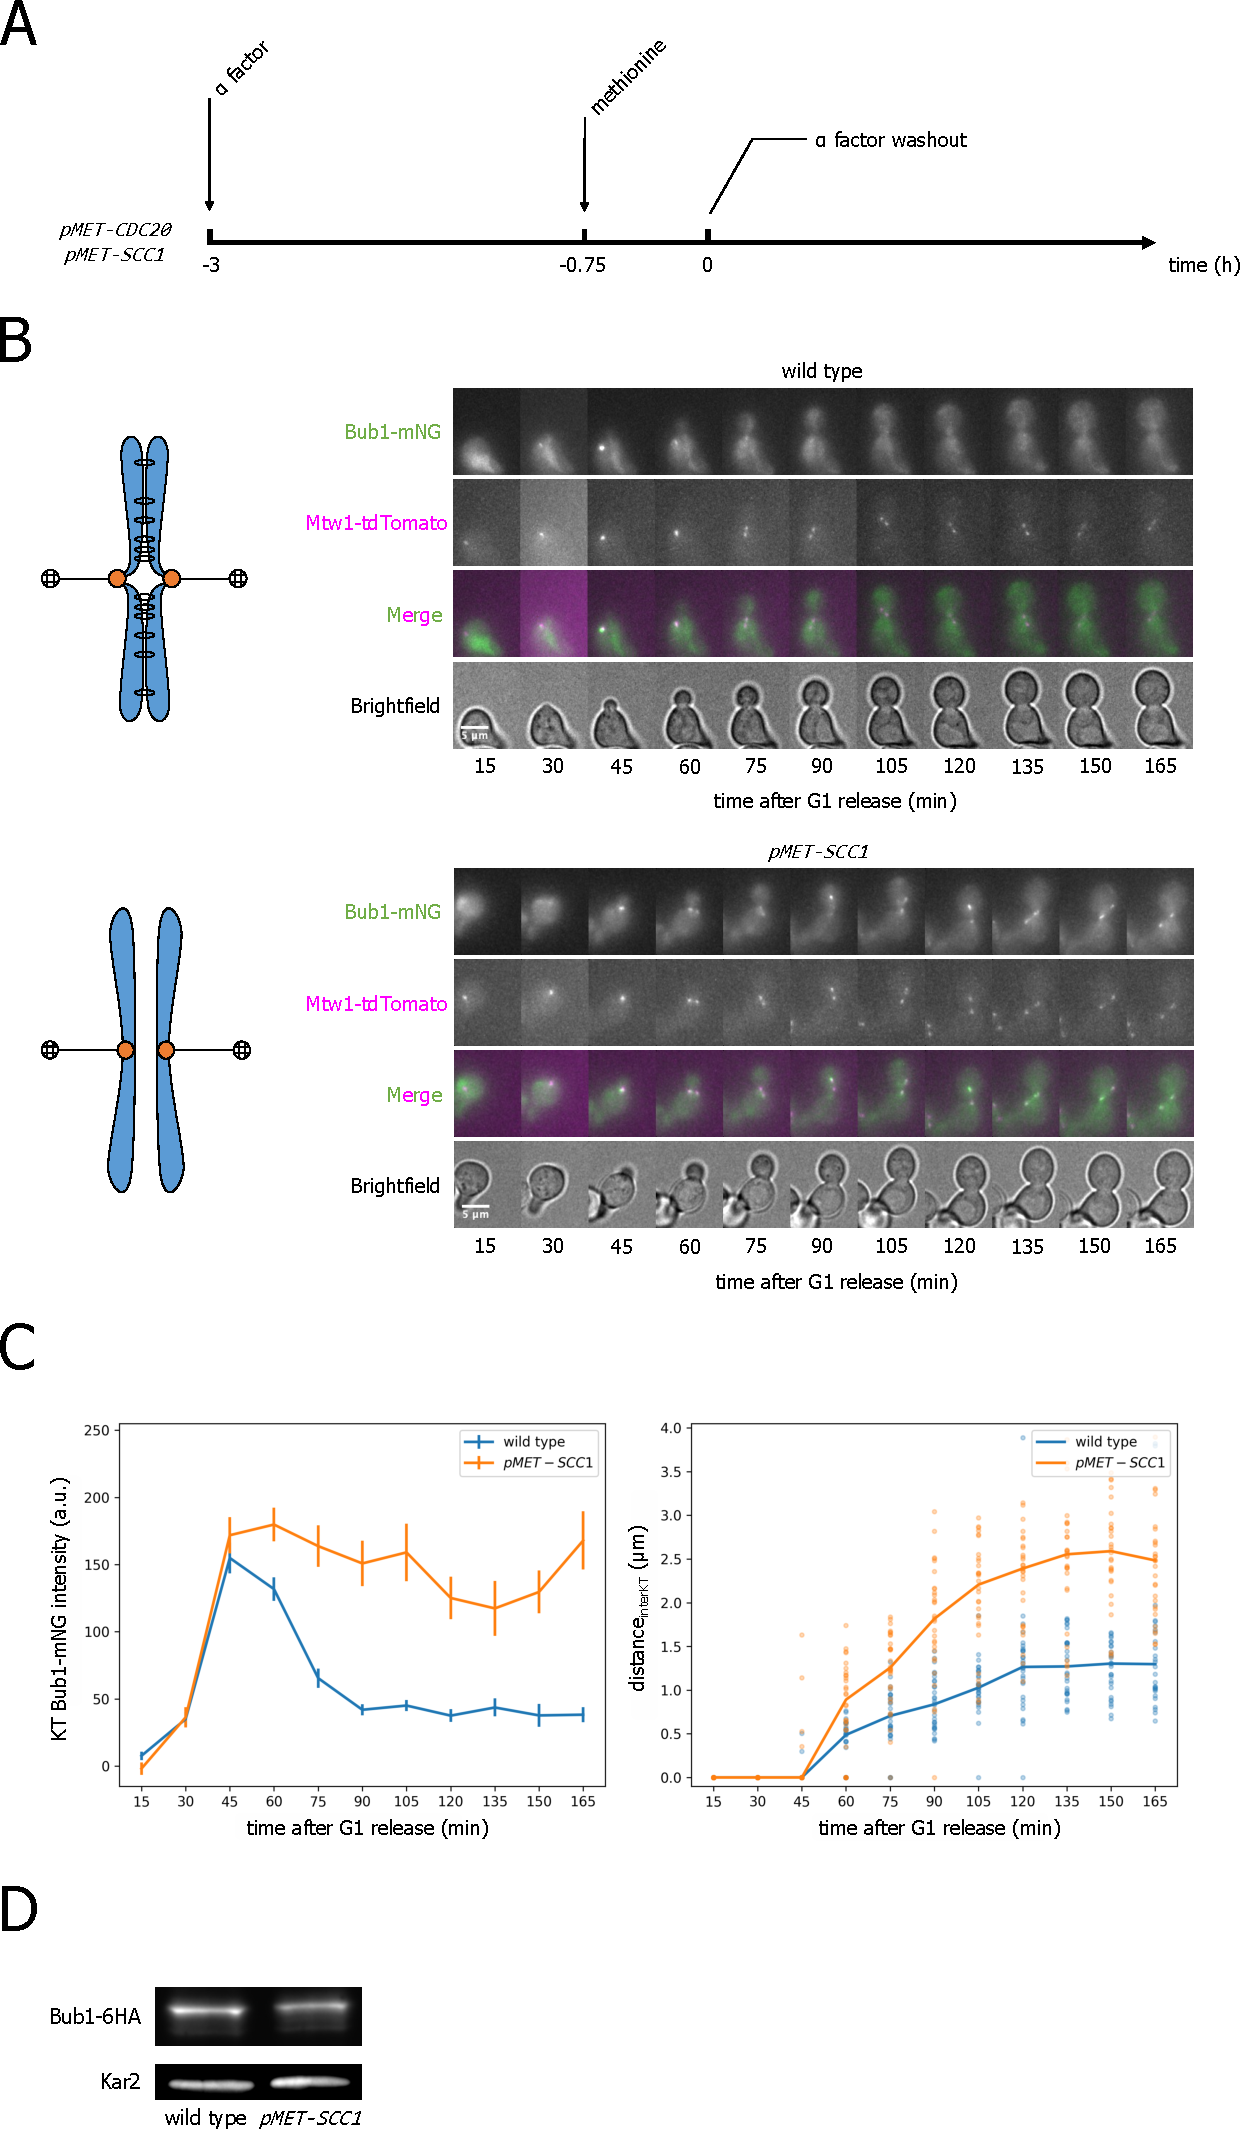
\includegraphics[width=0.9\textwidth]{chapter3/figures/Bub1-mNG pMET-SCC1.pdf}
  \caption[Tension is required for Bub1 re-localisation from the kinetochore]{Tension is required for Bub1 re-localisation from the kinetochore. (A) Schematics of experimental procedures. (B) Montage of representative time-lapse imaging. Cartoons on the left indicate the status of sister chromatids. (C) N=30 cells for each strain were followed over time and quantified for kinetochore Bub1-mNG fluorescence intensity and inter-kinetochore distance. Left panel: mean fluorescence intensity of Bub1-mNG at the kinetochore as a function of time. The error bar represents the standard error. Right panel: Median inter-kinetochore distance as a function of time. Individual data points are shown as dots. The wild type is shown in blue and \textit{pMET-SCC1} is shown in orange. (D) Western blotting with anti-HA antibody to detect Bub1 protein. Kar2 was used as the loading control. }
  \label{fig:bub1metscc1}
\end{figure} 

\subsection{Bub1 removal is sufficient for rapid de-localisation of Sgo1}
\cite{Nerusheva2014} have shown with ChIP-qPCR that Bub1 depletion abolishes Sgo1 localisation at the peri-centromere in the absence of tension, suggesting Bub1 removal triggers Sgo1 de-localisation. However, the 1 \si{\hour} time resolution of the experiment was not fine enough to explain the fast kinetics of Sgo1 re-localisation, where the transition from focused to diffused signal happens within 15 \si{\minute}. To repeat this result with an independent method as well as to improve the time resolution, I sought to repeat this experiment with microscopy. \textit{SGO1-EGFP MTW1-tdTomato pMET-CDC20} strain with additional AID system to deplete Bub1 (\textit{BUB1-3V5-AID} P$_{ADH1}$\textit{-OsTIR1-9MYC}) was synchronised in G1 and then released into nocodazole-containing media for a metaphase arrest without tension. Since Bub1 is a component of SAC, the media also does not contain methionine to prevent anaphase onset when Bub1 is depleted. Auxin NAA was then added to induce Bub1 depletion, with imaging started immediately (Figure~\ref{fig:bub1aid}A). Consistent with previous research, nocodazole-arrested cells showed large buds and signals of 2 or 3 dots for both Sgo1-EGFP and Mtw1-tdTomato \citep{Richmond2013Slk19Attachment}. In contrast to the control where DMSO was added (-NAA), Sgo1-EGFP foci disappeared after the addition of NAA (+NAA) (Figure~\ref{fig:bub1aid}C). Survival analysis indicated that the probability for cells to have a Sgo1-EGFP dot-signal started to decrease since NAA was added, with less than 20\% at 30 \si{\minute} afterwards (Figure~\ref{fig:bub1aid}D). To verify the depletion of Bub1 as well as characterising its kinetics, I performed western blotting on time course samples of cells treated identically as in the imaging experiment. The level of Bub1 protein became largely reduced at 20 \si{\minute} and barely detectable from 30 \si{\minute} after adding NAA (Figure~\ref{fig:bub1aid}E), similar to the dynamics of Sgo1 de-localisation shown in Figure~\ref{fig:bub1aid}D. This suggests a very quick response of Sgo1 localisation to Bub1 depletion, which could explain the fast re-localisation of Sgo1 previously observed \citep{Nerusheva2014}. Therefore, it is possible that the tension-dependent re-localisation of Sgo1 results from the de-localisation of Bub1 from the kinetochore by tension. 

\nomenclature{AID}{Auxin-Inducible Degron}
\nomenclature{NAA}{Naphthalene Acetic Acid}
\nomenclature{DMSO}{DiMethyl SulfOxide}

\begin{figure}[htbp]
  \centering
  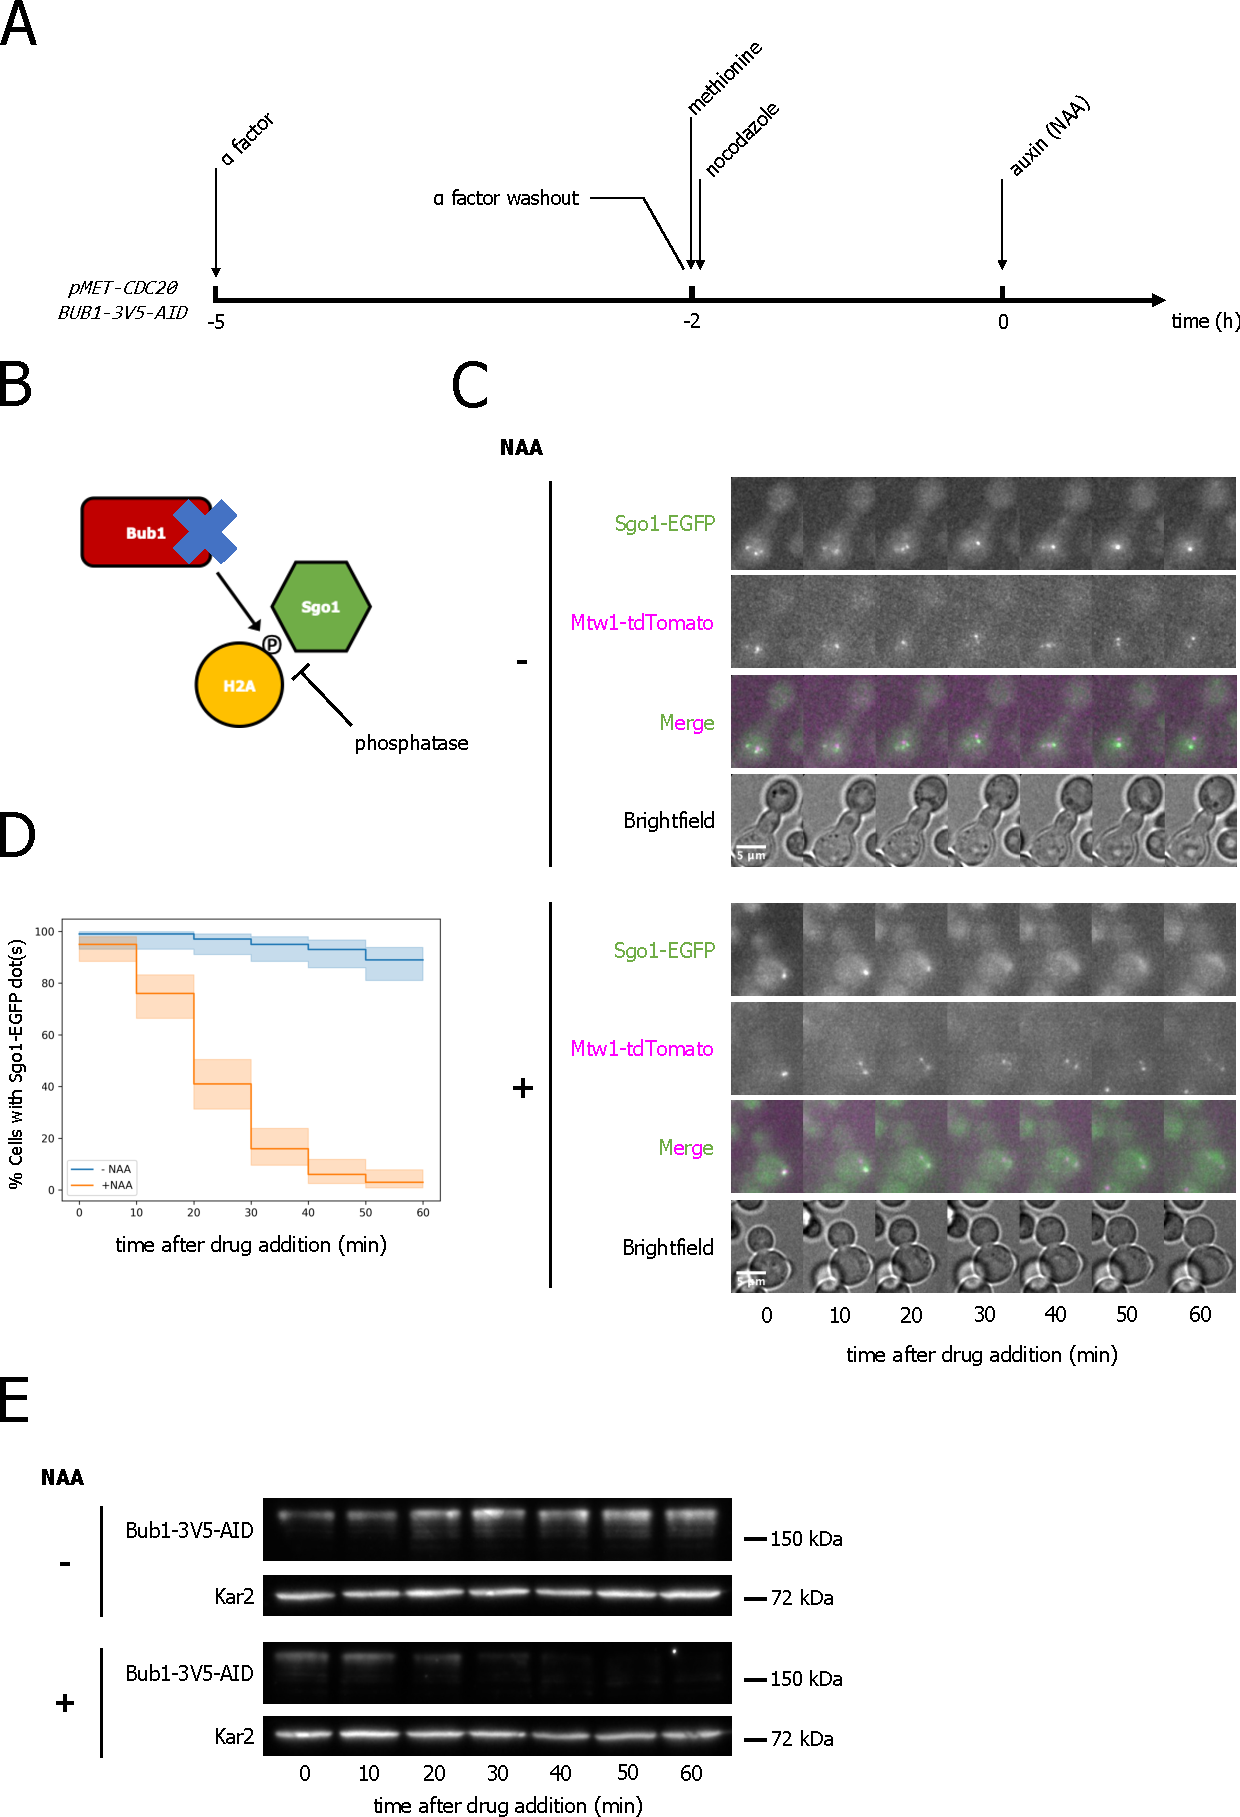
\includegraphics[width=0.9\textwidth]{chapter3/figures/Bub1-3V5-AID.pdf}
  \caption[Sgo1 is de-localised promptly upon Bub1 depletion in the absence of tension]{Sgo1 is de-localised promptly upon Bub1 depletion in the absence of tension. (A) Schematics of experimental procedures. (B) Schematics of experimental concept. (C) Montage of representative time-lapse imaging. (D) Survival analysis of the duration of focused Sgo1-EGFP signal. N=100 cells for each strain were followed over time and quantified for the duration of the Sgo1-EGFP signal being focused. Solid lines are Kaplan-Meier survival estimates. The shaded area in the same colour is the 95\% confidence limit of the estimate. (E) Western blotting with anti-V5 antibody to detect Bub1 protein. Kar2 was used as the loading control.}
  \label{fig:bub1aid}
\end{figure} 

\subsection{Bub1 re-localisation is earlier than Sgo1 re-localisation}
The data so far have suggested a model where Bub1 and Sgo1 re-localise sequentially. If this is true, there could be a difference in the timing of their re-localisation. To test it, a strain with the two proteins tagged with fluorescence proteins of different colours should be used in the ideal situation. However, none of Bub1 or Sgo1 tagged with various RFPs gave good enough signals under our microscope, possibly due to a combination of low abundance and cell-cycle-dependent expression of the two proteins. For example, Sgo1 tagged with the brightest RFP in the lab tdTomato is visible as dots in cells arrested with nocodazole but not in an unperturbed cell cycle because tdTomato has a maturation time beyond the time Sgo1 can be detected in a mitotic time course \citep{Indjeian2005a}. Instead, I could only image Bub1-mNG and Sgo1-EGFP in separate strains and use the inter-kinetochore distance measured from Mtw1-tdTomato as the internal control for timing. Standard G1 to metaphase live-cell imaging was carried out (Figure~\ref{fig:bub1sgo1}A). The inter-kinetochore distances are indistinguishable between the two strains (Figure~\ref{fig:bub1sgo1}B), suggesting a similar progress of tension establishment. Kinetochore Bub1-mNG fluorescence intensity was quantified as in the previous experiments. Due to the fact that Sgo1-EGFP is close to but does not co-localise with the kinetochore, it was not able to define the ROI to quantify fluorescence intensity. Therefore, Sgo1-EGFP was only scored for whether the signal can be counted as focused or not. Consistent with the speculation, the dynamics of Sgo1-EGFP and Bub1-mNG were similar except for a 15 \si{\minute} delay of Sgo1-EGFP in both the increase and decrease (Figure~\ref{fig:bub1sgo1}B), supporting the idea that Bub1 removal from the kinetochore triggers the de-localisation of Sgo1. 

\nomenclature{ROI}{Region Of Interest}

\begin{figure}[htbp]
  \centering
  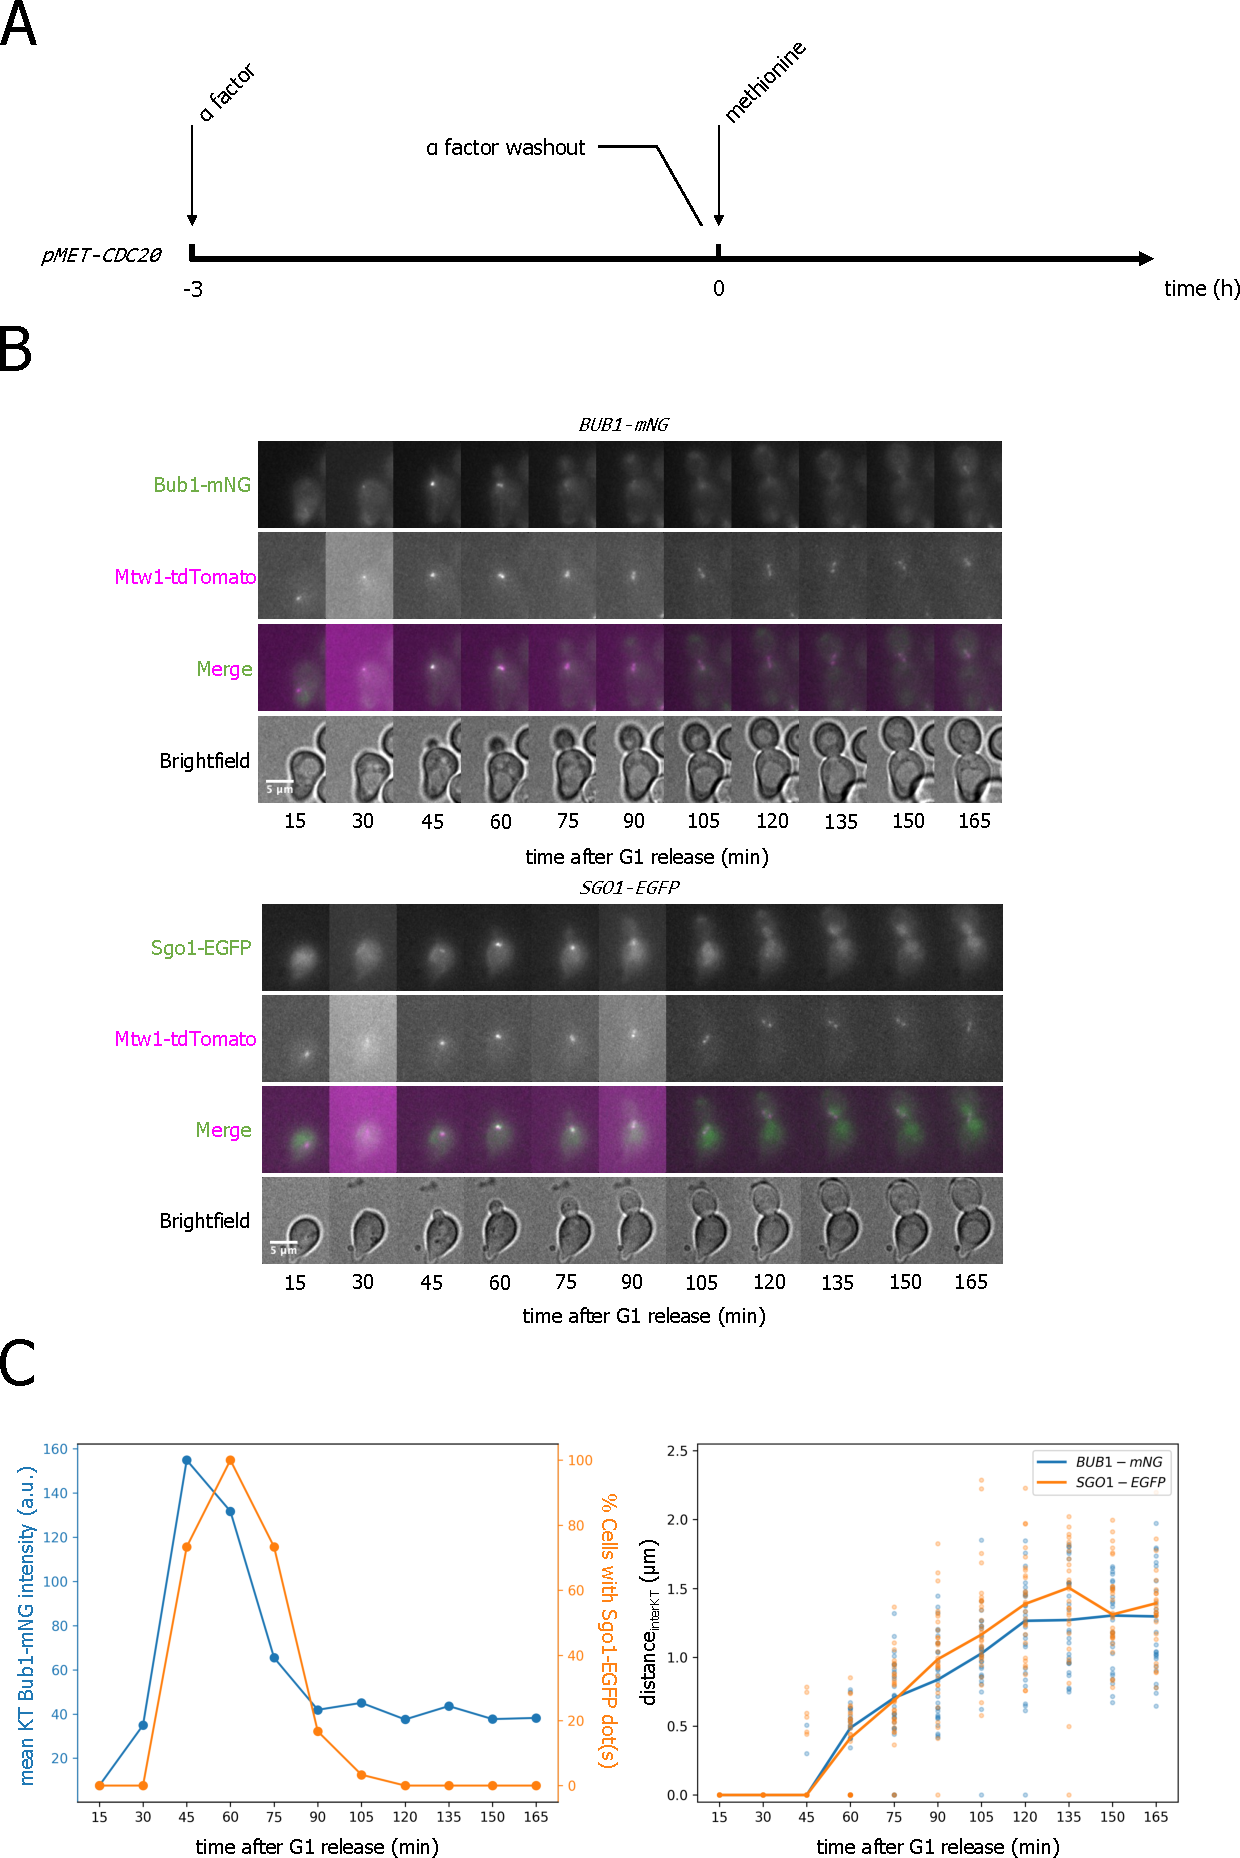
\includegraphics[width=0.9\textwidth]{chapter3/figures/Bub1-mNG Sgo1-EGFP.pdf}
  \caption[Bub1 is re-localised earlier than Sgo1]{Bub1 is re-localised earlier than Sgo1. (A) Montage of representative time-lapse imaging. (B) N=30 cells for each strain were followed over time and quantified. Left panel: mean fluorescence intensity of Bub1-mNG at the kinetochore and percentage of cells with Sgo1 foci as a function of time. Right panel: Median inter-kinetochore distance as a function of time. Individual data points are shown as dots. The \textit{BUB1-mNG} strain is shown in blue and the \textit{SGO1-EGFP} strain is shown in orange.}
  \label{fig:bub1sgo1}
\end{figure} 

\subsection{The continued presence of Bub1 is required to maintain H2A-pS121}
Our naive model argues that the phosphorylation status of the key substrate(s) determining Sgo1 localisation should be regulated by the kinase-phosphatase balance between Bub1 and unknown phosphatase(s) (Figure~\ref{fig:naive}). Therefore, the substrate(s) is expected to be phosphorylated in the absence of tension and de-phosphorylated when existing Bub1 is depleted as in the previous experiment (Figure~\ref{fig:ph2abub1aid}B). Given the demonstrated role of H2A-pS121 in localising Sgo1 to the peri-centromere \citep{Kawashima2010a, Fernius2007Bub1Mitosis, Nerusheva2014}, I hypothesised that it is the key Bub1 substrate being regulated. To directly monitor the phosphorylation status of H2A-S121, I ordered phospho-specific antibodies from Genscript. Western blotting using these antibodies indicated that they are able to distinguish phosphorylated H2A-S121 from unphosphorylated one as there is a less-than-17-\si{\kilo\dalton} band bright in wild type but extremely dim in Bub1 kinase-dead mutant (\textit{bub1$\Delta$K}) or H2A phospho-null mutant (H2A-S121A) arrested by nocodazole (Figure~\ref{fig:abtest}). 

\begin{figure}[htbp]
  \centering
  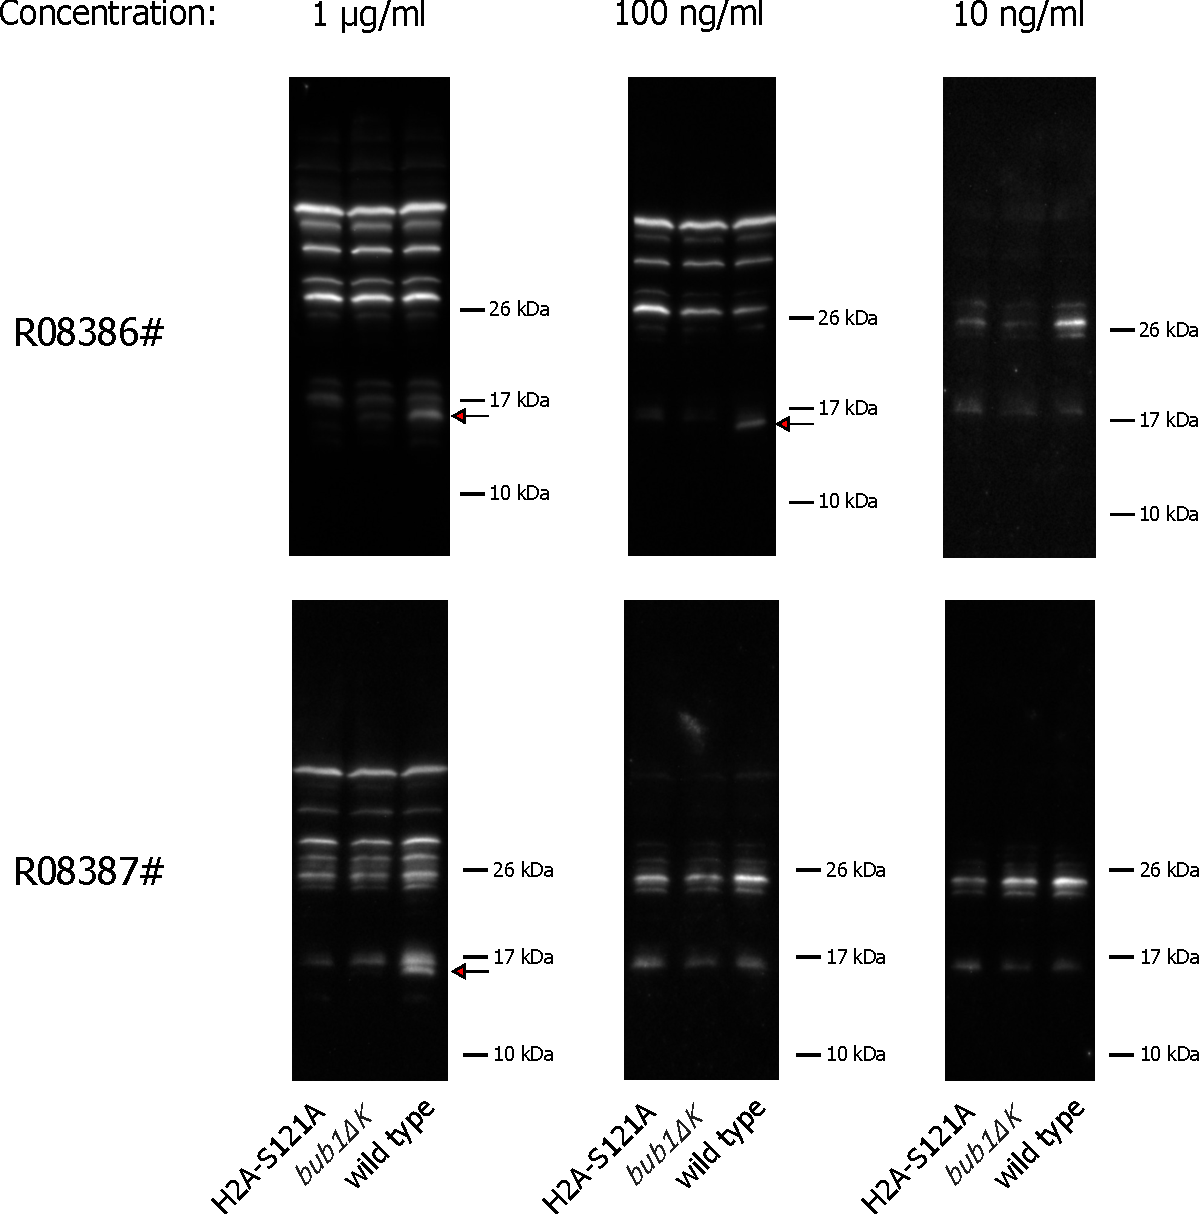
\includegraphics[width=0.9\textwidth]{chapter3/figures/pH2A ab test.pdf}
  \caption[Validation of phospho-specific antibodies for H2A-pS121]{Validation of phospho-specific antibodies for H2A-pS121. Western blotting on H2A-S121A, \textit{bub1$\Delta$K} or wild type arrested by nocodazole using anti-Hta2-pS122 antibodies generated from host R08386\# or R08387\# (GenScript) at 1 \si{\micro\gram/\milli\litre}, 100 \si{\nano\gram/\milli\litre} or 10 \si{\nano\gram/\micro\litre}. Red arrows indicate the specific bands. }
  \label{fig:abtest}
\end{figure} 

To test whether H2A is indeed de-phosphorylated at S121 upon Bub1 depletion, I conducted western blotting on samples from the experiment of Figure~\ref{fig:bub1aid} (Figure~\ref{fig:ph2abub1aid}A). The specific band is maintained within the scope of the experiment in -NAA samples. In contrast, it is reduced in +NAA samples in spite of the increase in the intensity of the non-specific band above (Figure~\ref{fig:ph2abub1aid}C), suggesting that H2A-pS121 is being de-phosphorylated due to Bub1 depletion. Hence, the continued presence of Bub1 is required to maintain H2A-pS121, favouring the naive model and the idea that H2A-pS121 is the key substrate. Due to the non-ideal specificity of the antibody over unphosphorylated H2A-S121, it is difficult to interpret the kinetics of the de-phosphorylation. 

\begin{figure}[htbp]
  \centering
  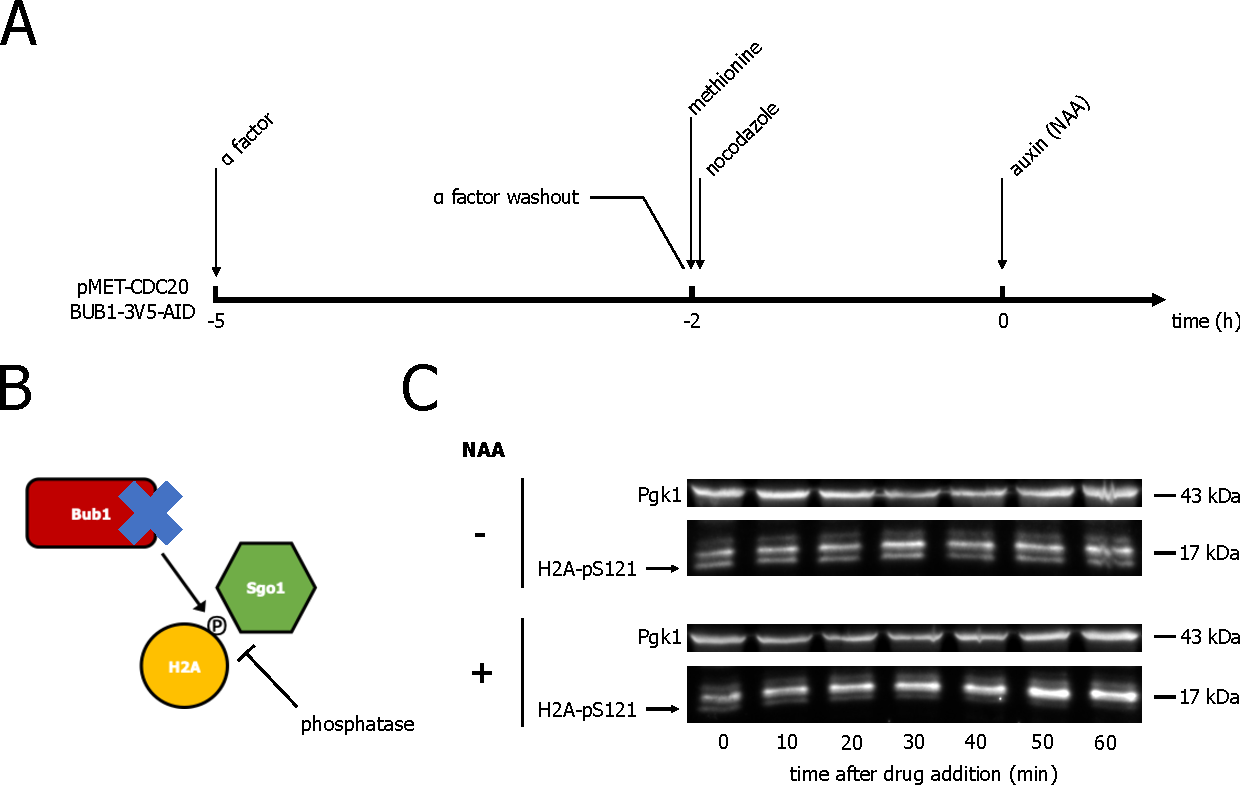
\includegraphics[width=0.9\textwidth]{chapter3/figures/pH2A Bub1-AID.pdf}
  \caption[Bub1 depletion leads to a reduction in H2A-S121 phosphorylation in the absence of tension]{Bub1 depletion leads to a reduction in H2A-S121 phosphorylation in the absence of tension. (A) Schematics of experimental procedures. (B) Schematics of experimental concept. (C) Western blotting with anti-H2A-pS121 antibody to detect the phosphorylation status of H2A. Pgk1 was used as the loading control.}
  \label{fig:ph2abub1aid}
\end{figure} 

\subsection{Total cellular H2A-pS121 level is independent of tension}
\label{subsec:totalph2aindten}

Since tension de-localises Bub1 from the kinetochore, physically separating it from its substrate H2A at the peri-centromere, I hypothesised that the phosphorylation of H2A-S121 would be lost or at least reduced by tension. Therefore, I arrested wild type strain, the control strain used for imaging and the negative control \textit{bub1$\Delta$K} in the presence or absence of tension (Figure~\ref{fig:ph2atension}A). Western blotting against H2A-pS121 was conducted as before. Surprisingly, tension did not decrease the intensity of the specific band for both wild type and the imaging strain (Figure~\ref{fig:ph2atension}B), indicating the level of total cellular H2A-pS121 is independent of tension. It seems that tension even increased the specific band intensity for the imaging strain. However, I believe it is due to the variation in the blotting process, as the intensity of the non-specific band is also reduced in the no tension sample compared to the tension sample. 

\begin{figure}[htbp]
  \centering
  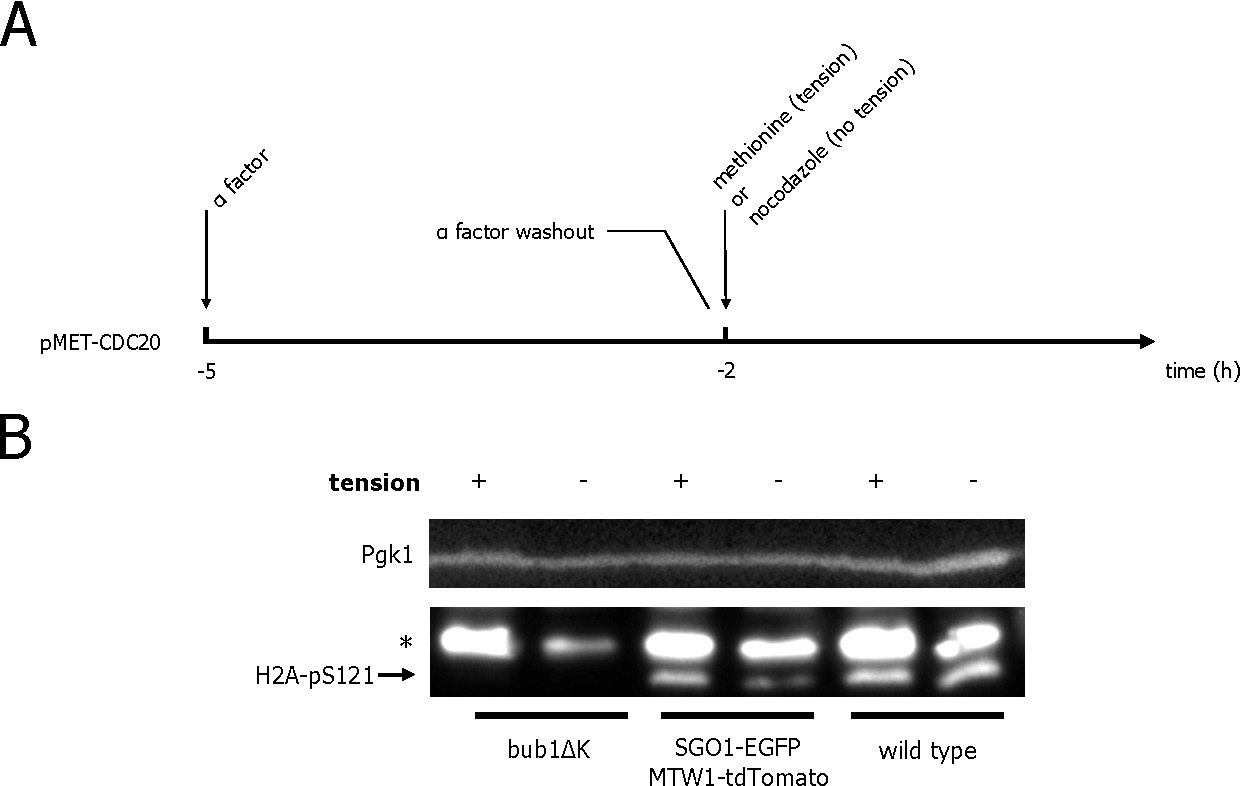
\includegraphics[width=0.9\textwidth]{chapter3/figures/pH2A tension.pdf}
  \caption[Total cellular H2A-pS121 level is independent of tension]{Total cellular H2A-pS121 level is independent of tension.(A) Schematics of experimental procedures. (B) Western blotting with anti-H2A-pS121 antibody to detect the phosphorylation status of H2A. Pgk1 was used as the loading control. The asterisk represents the non-specific band.}
  \label{fig:ph2atension}
\end{figure}

To validate this unexpected result, I turned to a different approach where H2A-pS121 were monitored over the entire cell cycle. Cells bearing \textit{PDS1-HA} were synchronised in G1 and released into rich media as described in the previous synchronised mitotic time course experiment (Figure~\ref{fig:ph2atimecourse}A). Tubulin IF indicated that most cells were in metaphase at 75 \si{\minute} after G1 release while in anaphase at 90 and 105 \si{\minute} (Figure~\ref{fig:ph2atimecourse}B). Western blotting with anti-HA and anti-H2A-pS121 was then performed on the time course samples. The securin Pds1 peaked at 75 \si{\minute} and became barely visible at 90 \si{\minute}, consistent with the cell cycle stages information from the tubulin IF. The H2A-pS121 band was comparable from 60 to 90 \si{\minute}, with a sharp reduction at 105 \si{\minute}, suggesting the level of H2A-pS121 is maintained during the metaphase-anaphase transition, therefore verifying the previous result. The reason that the non-specific bands here appeared differently from the previous experiments is likely due to the fact that I used a large protein gel in this western blotting for better protein resolution. Interestingly, the dynamics of H2A-pS121 level over the cell cycle are qualitatively similar to that of Bub1 protein level (Figure~\ref{fig:bub1timecourse}). 

\begin{figure}[htbp]
  \centering
  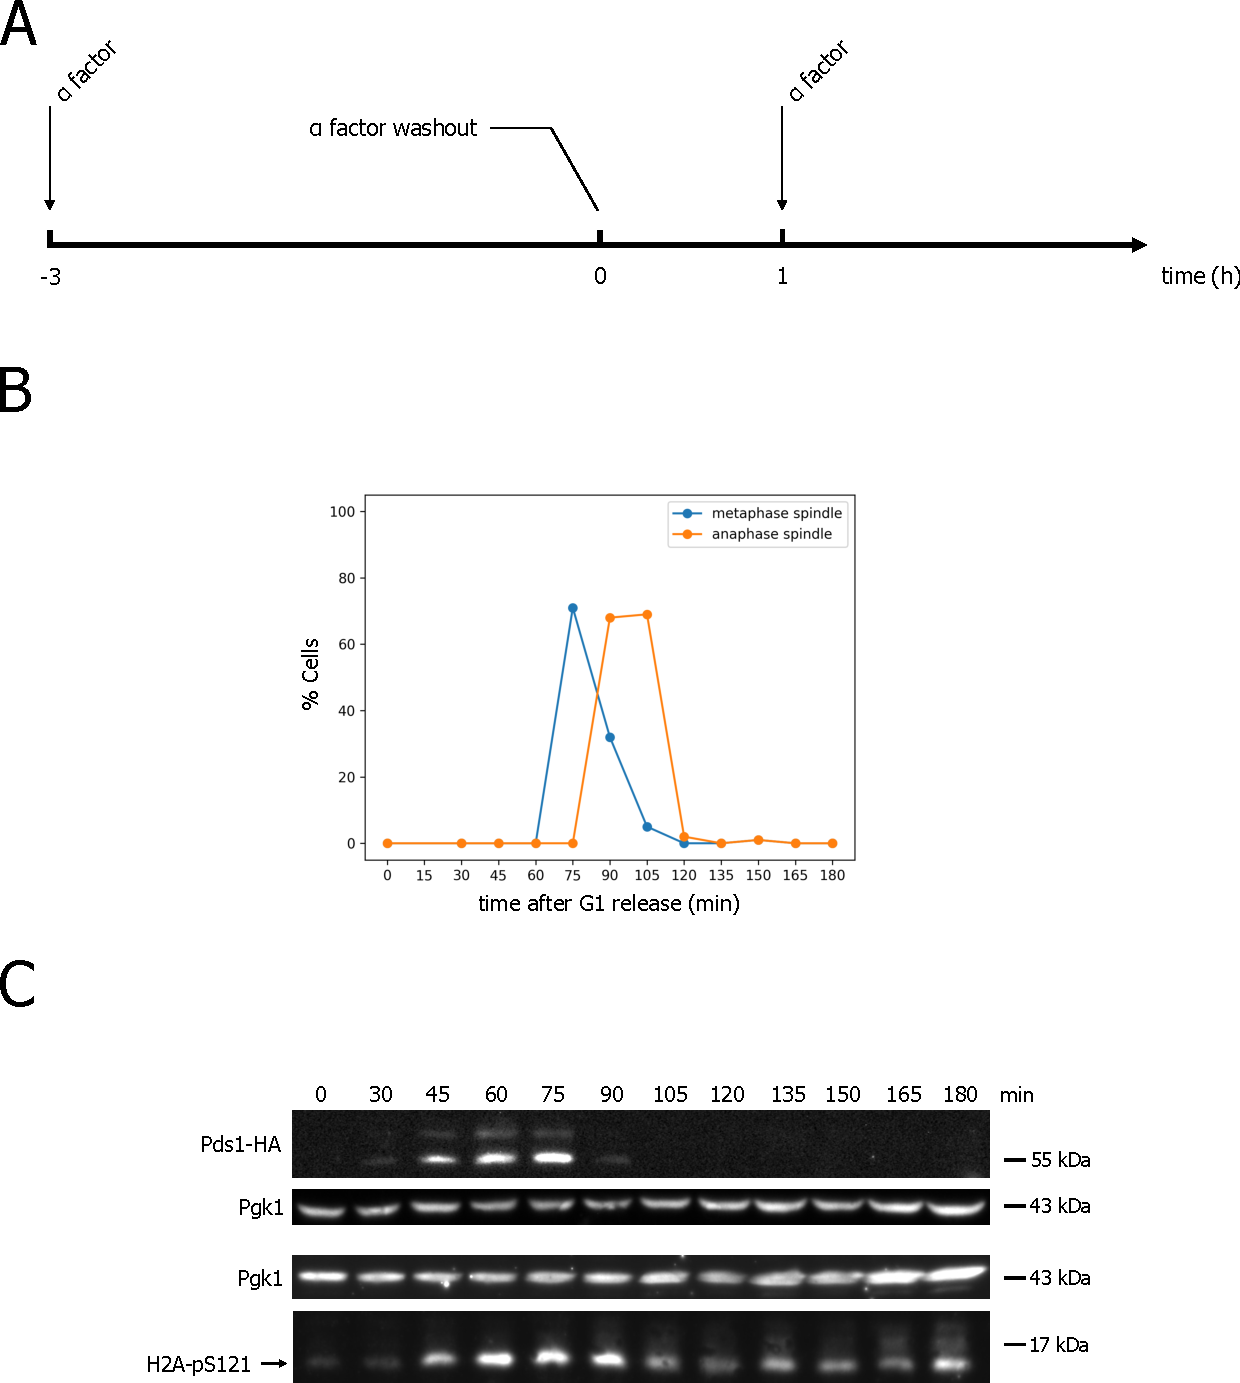
\includegraphics[width=0.9\textwidth]{chapter3/figures/pH2A mitotic time course.pdf}
  \caption[H2A-pS121 level is maintained during metaphase-anaphase transition]{H2A-pS121 level is maintained during metaphase-anaphase transition. (A) Schematics of experimental procedures. (B) The proportion of cells with metaphase or anaphase spindle over time by tubulin IF. (C) Upper: western blotting with anti-HA antibody to detect Pds1 protein. Pgk1 was used as the loading control. Lower: western blotting with anti-H2A-pS121 antibody to detect the phosphorylation status of H2A. Pgk1 was used as the loading control.}
  \label{fig:ph2atimecourse}
\end{figure}

\subsection{Tension re-distributes H2A-pS121 from the centromere to the chromosome arm}

Intuitively, the total level of H2A-pS121 being unaffected by tension contradicts the previous finding that its maintenance requires continued Bub1 and Bub1 is de-localised from the kinetochore upon tension. However, one possibility that can explain both is that de-localised Bub1 reaches and phosphorylates H2A molecules other than the ones localised at the peri-centromere whereas the previously phosphorylated ones at the peri-centromere started to be de-phosphorylated, resulting in a change in the localisation of H2A-pS121 but not the total level. To test this hypothesis, we sought to conduct either IF or ChIP using the H2A-pS121 phospho-specific antibody. Considering the poor specificity of the antibody, I turned to ChIP because it is supposed to provide a better signal-to-noise ratio. 

First, I carried out a test ChIP-qPCR to determine whether the antibody can be used for ChIP as well as the optimal fixing time. tension-less metaphase wild type or \textit{bub1$\Delta$K}, the negative control, cells arrested by nocodazole were fixed for 10, 20, 30 and 60 \si{\minute}. Samples were then subject to ChIP with the anti-H2A-pS121 antibody and qPCR was used to determine the enrichment at the centromere, chromosome arm and peri-centromere of chromosome IV. Signals were detected at the centromere and peri-centromere in wild type but not in \textit{bub1$\Delta$K}, showing that the antibody is capable of ChIP application. Consistent with the localisation in vertebrates by IF experiments \citep{Ricke2012, Kawashima2010a, Liu2013a, Williams2017Bub1Kinetochores, Zhang2020FunctioningMitosis, Liang2019ACells, Lee2008, Liu2015}, H2A-pS121 enrichment is vastly reduced on the chromosome arm in wild type. The fixing time does not seem to be important for this particular experiment. I decided to use 10 \si{\minute} as it should cross-link fewer irrelevant proteins to the DNA in theory and therefore reduce the likelihood of potential artefacts. 

\begin{figure}[htbp]
  \centering
  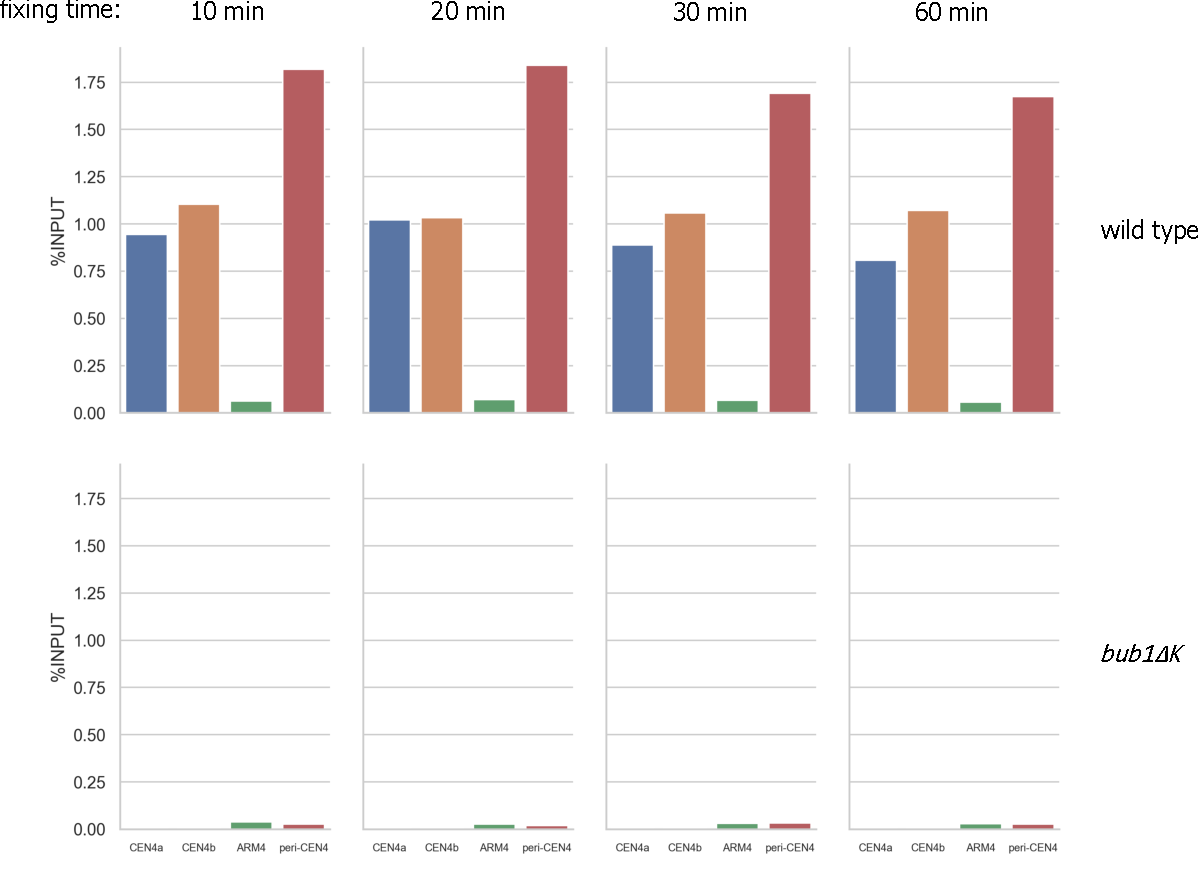
\includegraphics[width=0.9\textwidth]{chapter3/figures/pH2A test ChIP-qPCR.pdf}
  \caption[The H2A-pS121 phospho-specific antibody can be used for ChIP]{The H2A-pS121 phospho-specific antibody can be used for ChIP. Wild type and \textit{bub1$\Delta$K} cells arrested in metaphase without tension were fixed for 10, 20, 30 and 60 minutes, respectively, and subjected to H2A-pS121 ChIP-qPCR at 4 different loci, with two at the centromere, one at chromosome arm and one at the peri-centromere of chromosome IV. }
  \label{fig:ph2atestchipqpcr}
\end{figure}

Next, I conducted a formal H2A-pS121 ChIP-seq experiment. To be able to compare signals between samples, a wet calibration method was used, where the genome from another species, fission yeast in this case, was mixed with the budding yeast genome in the experiment \citep{Hu2015BiologicalChIP-seq}. Wild type cells were arrested in metaphase with or without tension (Figure~\ref{fig:ph2achipseqchecking}A). Tubulin IF indicated that they have good synchronisation. 98\% cells from the tension sample displayed metaphase spindle while none of the cells from the no tension sample showed a spindle (Figure~\ref{fig:ph2achipseqchecking}B). Western blotting was used to examine the level of H2A-pS121 in the two samples. Consistent with the previous results (Subsection~\ref{subsec:totalph2aindten}), both samples showed comparable band intensities (Figure~\ref{fig:ph2achipseqchecking}C). ChIP-processed samples were further checked by qPCR for the enrichment of budding and fission yeast's loci to ensure quality. Similar to the test qPCR, the no tension sample showed high signals at the centromere and peri-centromere but not on the chromosome arm. Consistent with the idea that tension might affect the localisation of H2A-pS121, the tension sample had low signals at all three loci (Figure~\ref{fig:ph2achipseqchecking}D). The amount of fission yeast cells used for calibration is the same between samples. Therefore, it is expected that both of them should give equal enrichment at a given locus. Indeed, the signals were comparable between samples at the centromere core and outer repeat of fission yeast (Figure~\ref{fig:ph2achipseqchecking}E). 

\begin{figure}[htbp]
  \centering
  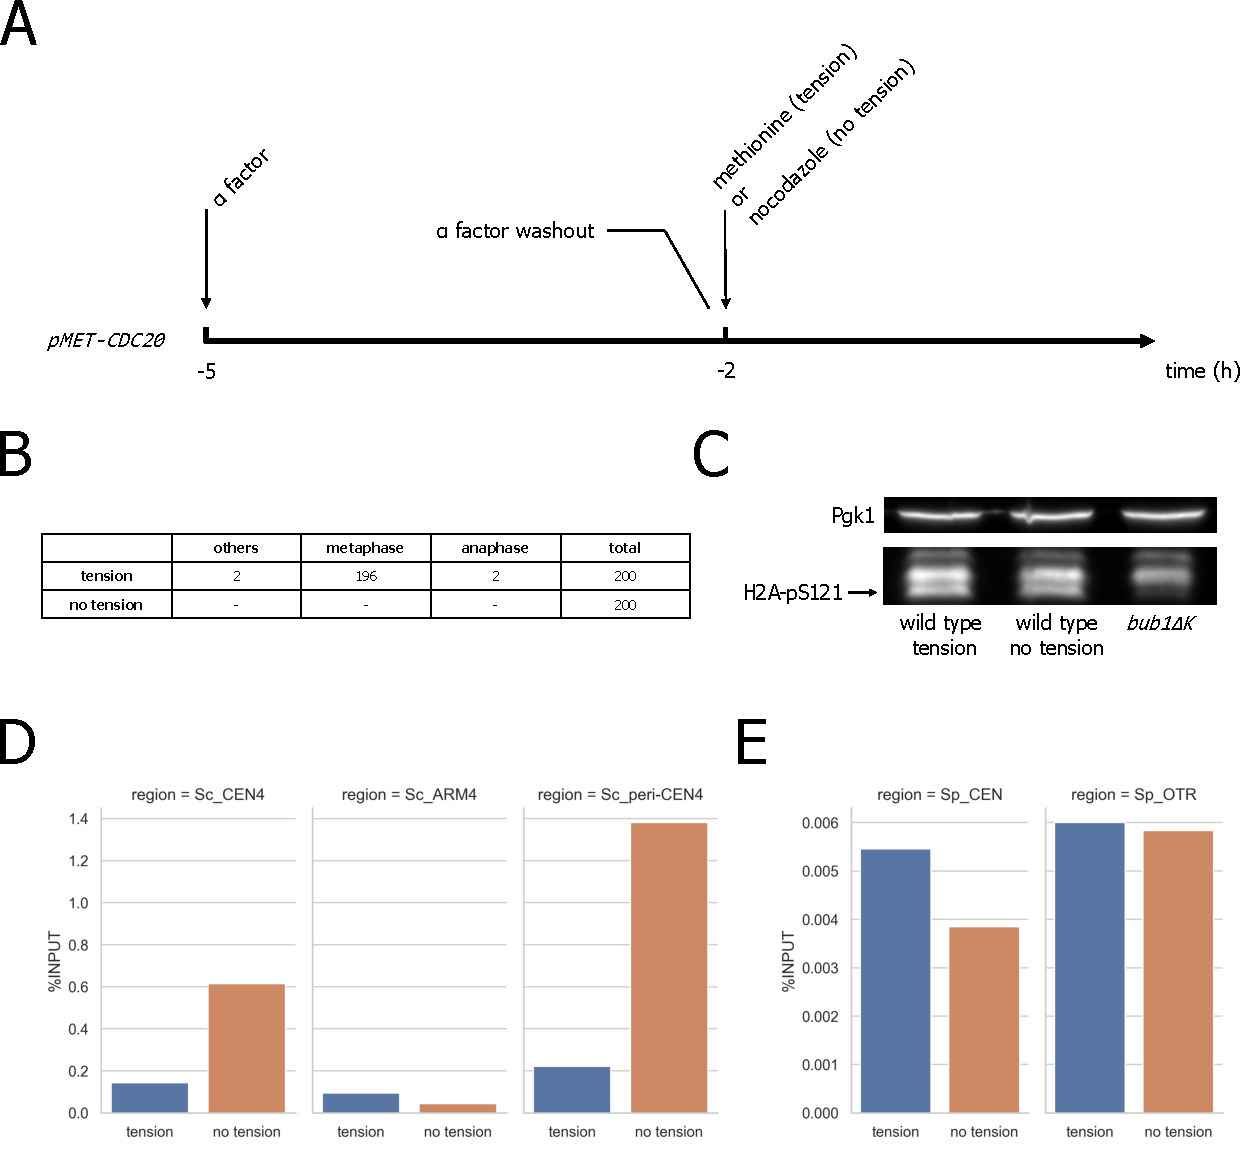
\includegraphics[width=0.9\textwidth]{chapter3/figures/checking.pdf}
  \caption[Quality control of calibrated H2A-pS121 ChIP-seq]{Quality control of calibrated H2A-pS121 ChIP-seq. (A) Schematics of experimental procedures. (B) Spindle morphology count by tubulin IF. (C) Western blotting with anti-H2A-pS121 antibody to detect the phosphorylation status of H2A. Pgk1 was used as the loading control. (D) H2A-pS121 ChIP-qPCR at the chromosome IV centromere, chromosome arm and peri-centromere of \textit{S.cerevisiae}. (E) H2A-pS121 ChIP-qPCR at chromosome I centromere core and outer repeat of \textit{S.pombe}. }
  \label{fig:ph2achipseqchecking}
\end{figure}

With quality control conducted, I proceeded with the ChIP samples and set up sequencing. The enrichment profile of a representative chromosome, chromosome IV, is shown in Figure~\ref{fig:ph2achipseq2nd}A. H2A-pS121 has a bell-shaped distribution at the centromere in both the tension and no tension sample. However, quantitatively, consistent with the result from qPCR, the signals were massively reduced in the tension sample. In contrast, on the chromosome arm, the signals were higher for the tension sample, supporting the hypothesis. This is confirmed by the pile-up of all 16 chromosomes. At centromeres, the signals of the tension sample were about a quarter of that of the no tension sample, whereas, on the arms, the former showed a roughly one-fold increase from the latter (Figure~\ref{fig:ph2achipseq2nd}B). To provide a more quantitative view, I categorised sequencing reads as either at centromeres or on the chromosome arms. Although the total number was similar, only 18\% of reads were assigned to the centromeres in the tension sample while the number is 63\% in the no tension sample (Figure~\ref{fig:ph2achipseq2nd}C). Hence, we concluded that the establishment of tension caused a re-distribution of H2A-pS121 from the centromere to the chromosome arm. 

\begin{figure}[htbp]
  \centering
  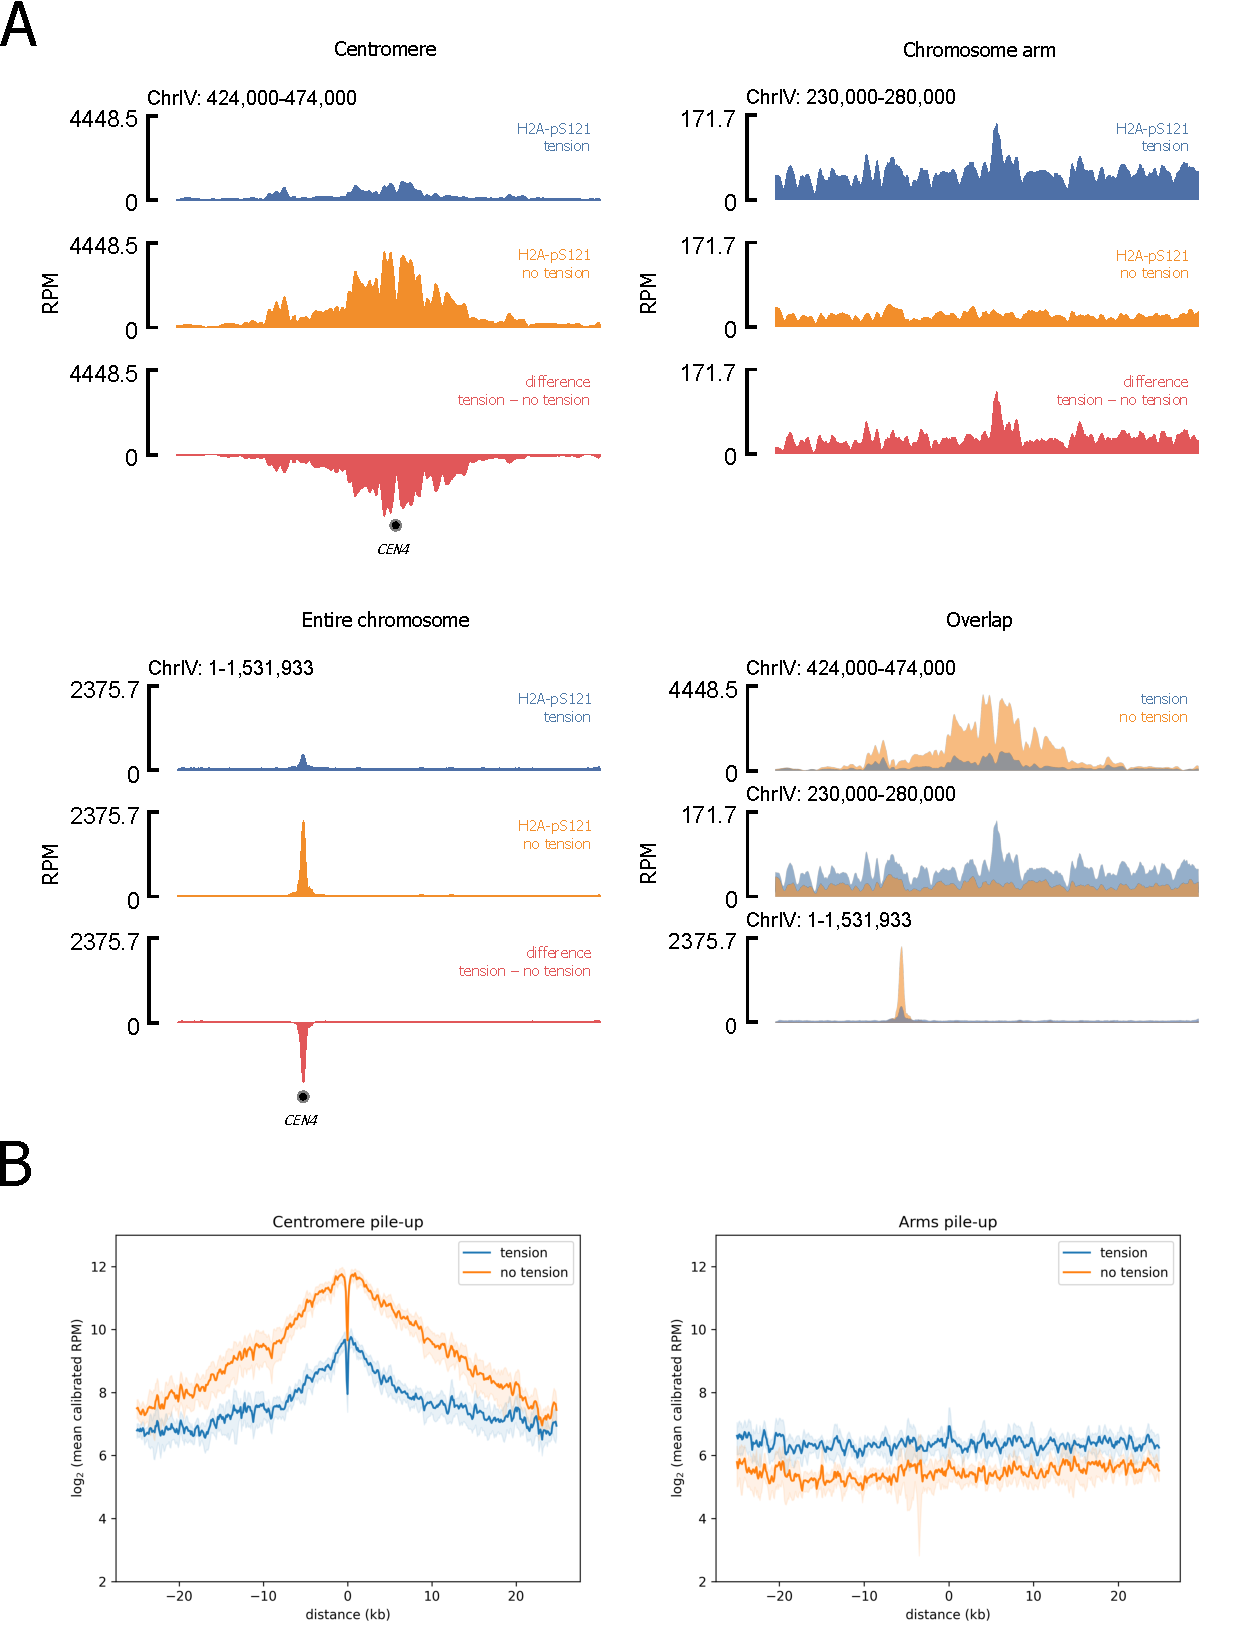
\includegraphics[width=0.9\textwidth]{chapter3/figures/pH2A ChIP-seq_1st.pdf}
\end{figure}

\begin{figure}[t]
  \centering
  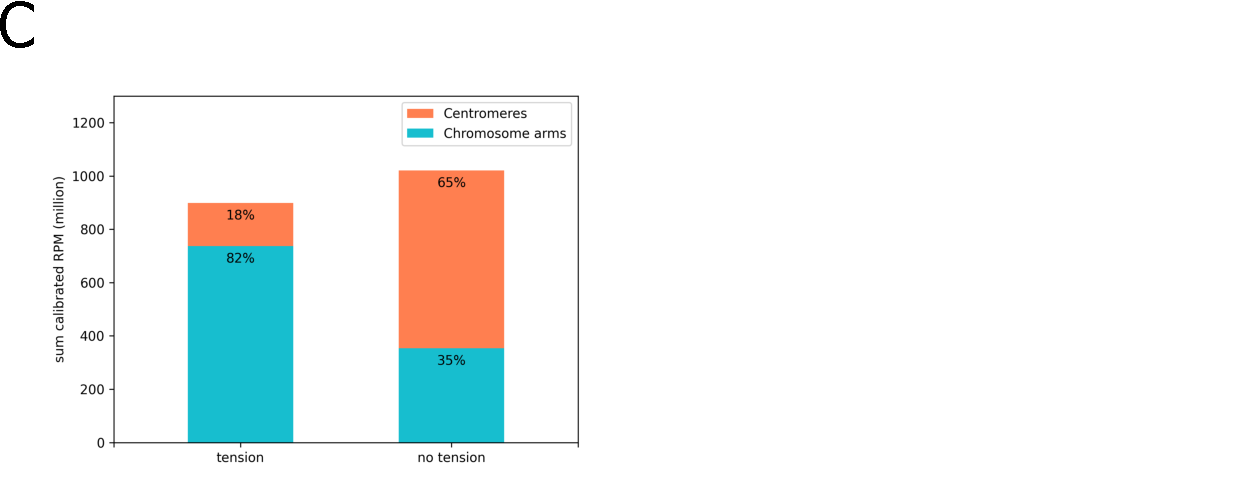
\includegraphics[width=0.9\textwidth]{chapter3/figures/pH2A ChIP-seq_2nd.pdf}
  \caption[H2A-pS121 is re-distributed from centromere to chromosome arm upon the establishment of tension]{H2A-pS121 is re-distributed from centromere to chromosome arm upon the establishment of tension. (A) Calibrated H2A-pS121 ChIP-seq profiles of cells arrested in metaphase with or without tension and their difference (tension - no tension) at the 50kb region around the centromere of chromosome IV (upper left), a 50kb region on the left arm of chromosome IV (upper right) and the entire chromosome IV (bottom left). The overlapped profiles are shown in the bottom right. (B) Pile-up of centromeres and chromosome arms. Left: the 50kb regions around the centromeres of all 16 chromosomes. Right: the 50kb regions around chromosome arms (80kb left to the centromere) of all 16 chromosomes. (C) The number of sequencing reads assigned to centromeres (the 50kb-region flanking the core centromere) or chromosome arms in each sample. }
  \label{fig:ph2achipseq2nd}
\end{figure}

\subsection{Sgo1 cannot be concentrated at the peri-centromere in H2A phospho-mimic mutant}

The re-distribution of H2A-pS121 upon tension points to a possibility that it triggers Sgo1 re-localisation. If it is true, The H2A phospho-mimic mutant whose mark for Sgo1 localisation spreads along the entire chromosome, and thus mimicking the tension situation, should lose its Sgo1 enrichment at peri-centromere in the absence of tension. However, \cite{Nerusheva2014} reported an opposite result and, combined with other results, eventually reached the conclusion that Bub1 has substrates other than H2A important for Sgo1 localisation. Due to a lack of supporting evidence from other species and the difficulty of making H2A mutants in budding yeast, I decided to verify the results by first sequencing the original strains used in the research. Surprisingly, The H2A phospho-mimic mutants turned out to be wild type for the HTA1 locus (Figure~\ref{fig:h2as121dseq}), consistent with the observation that strains with H2A-S121D mutations always show the same phenotype as wild type in the paper. 

\begin{figure}[htbp]
  \centering
  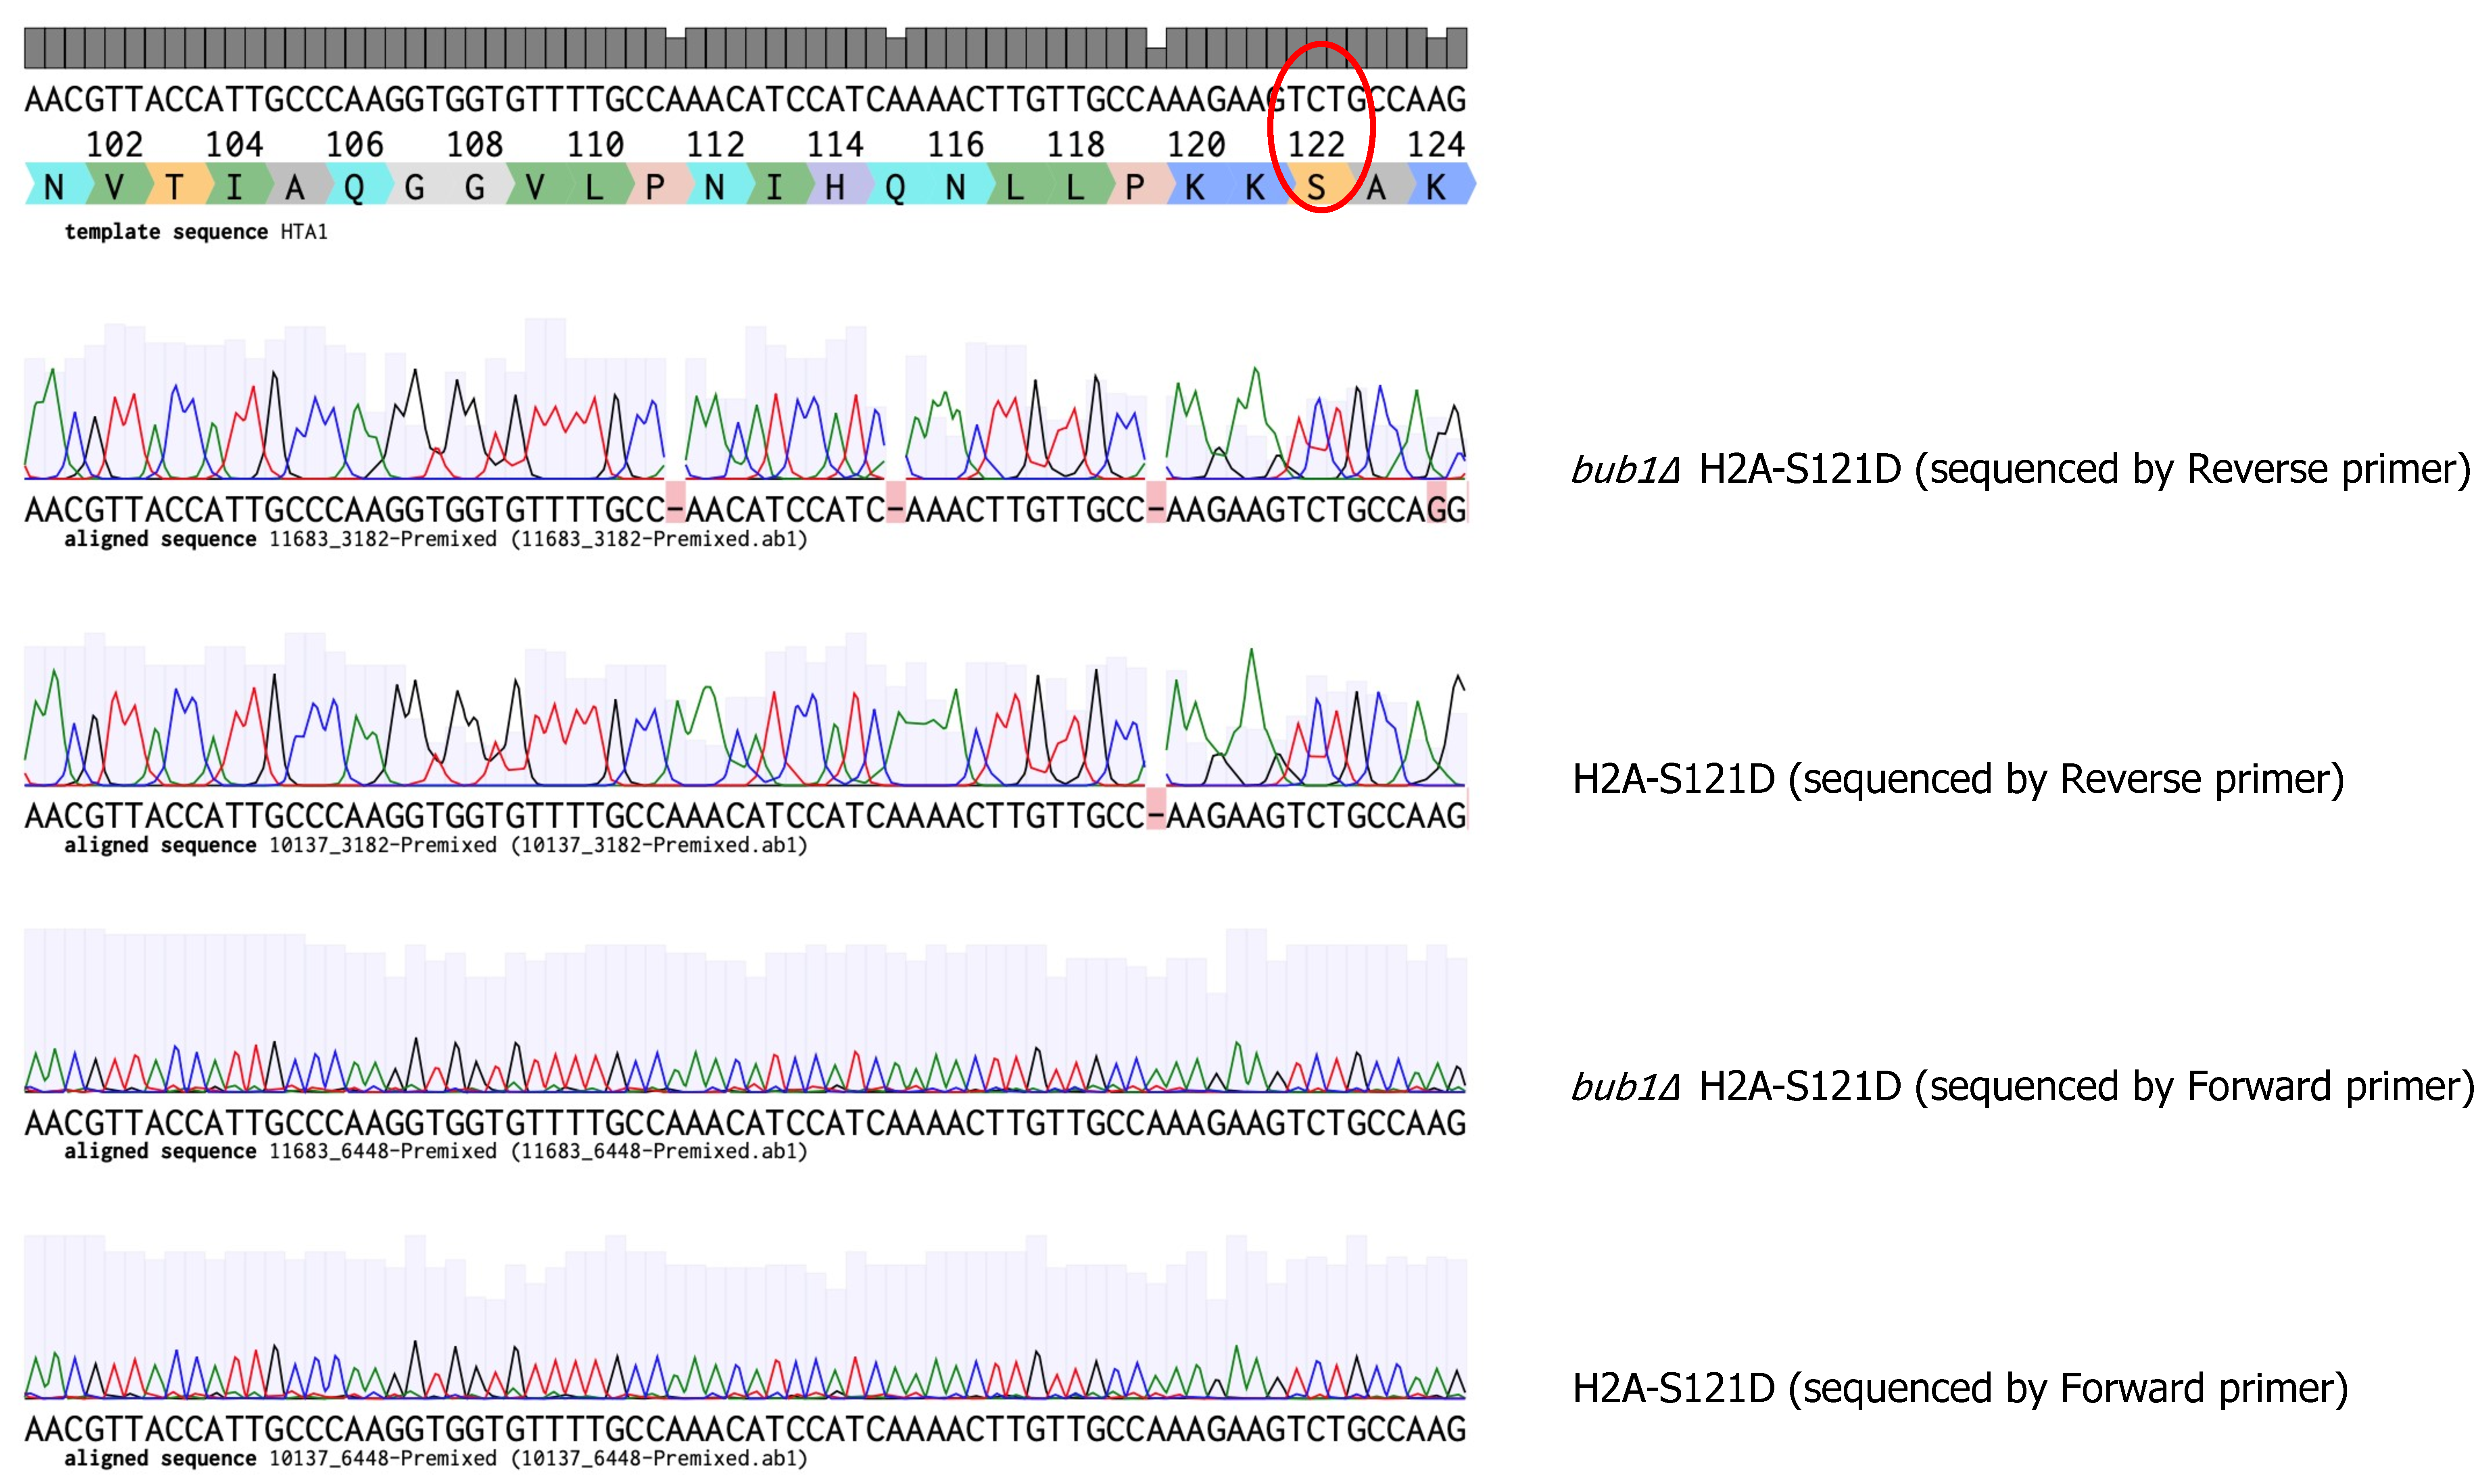
\includegraphics[width=0.9\textwidth]{chapter3/figures/nerusheva_sequencing.pdf}
  \caption[H2A phopho-mimic mutants used in \citep{Nerusheva2014} bear wild type sequence]{Phopho-mimic mutants used in \citep{Nerusheva2014} bear wild type sequence. The red circle indicates the expected mutation site.}
  \label{fig:h2as121dseq}
\end{figure}

To test whether Sgo1 localisation is altered in H2A phospho-mimic mutants, I re-constructed the strain and repeated the Sgo1-6HA ChIP-qPCR experiment by \cite{Nerusheva2014}. The standard cell harvesting procedure comparing tension with no tension conditions was performed on no tag, wild type, H2A-S121A, as a negative control, and H2A-S121D (Figure~\ref{fig:sgo1chiph2amutants}A). Tubulin IF indicated synchronised metaphase arrest in the tension samples and an absence of spindle in the no tension samples (Figure~\ref{fig:sgo1chiph2amutants}B). Western blotting showed comparable Sgo1 expression in wild type, H2A-S121A and H2A-S121D but not in no tag (Figure~\ref{fig:sgo1chiph2amutants}C). Samples then underwent ChIP processing and qPCR was used to determine the enrichment at the chromosome arm, peri-centromere and centromere of chromosome IV (Figure~\ref{fig:sgo1chiph2amutants}D). As expected, Sgo1 exhibited increased association with chromatin at the centromeric/ peri-centromeric region but not on the arm in wild type without tension. However, this increase was abolished in H2A-S121A or H2A-S121D, suggesting Sgo1 cannot be enriched at peri-centromere even in the absence of tension, supporting the idea that the phospho-mimic mutant resembles the scenario with established tension regarding Sgo1 localisation (Figure~\ref{fig:sgo1chiph2amutants}E). 

\begin{figure}[htbp]
  \centering
  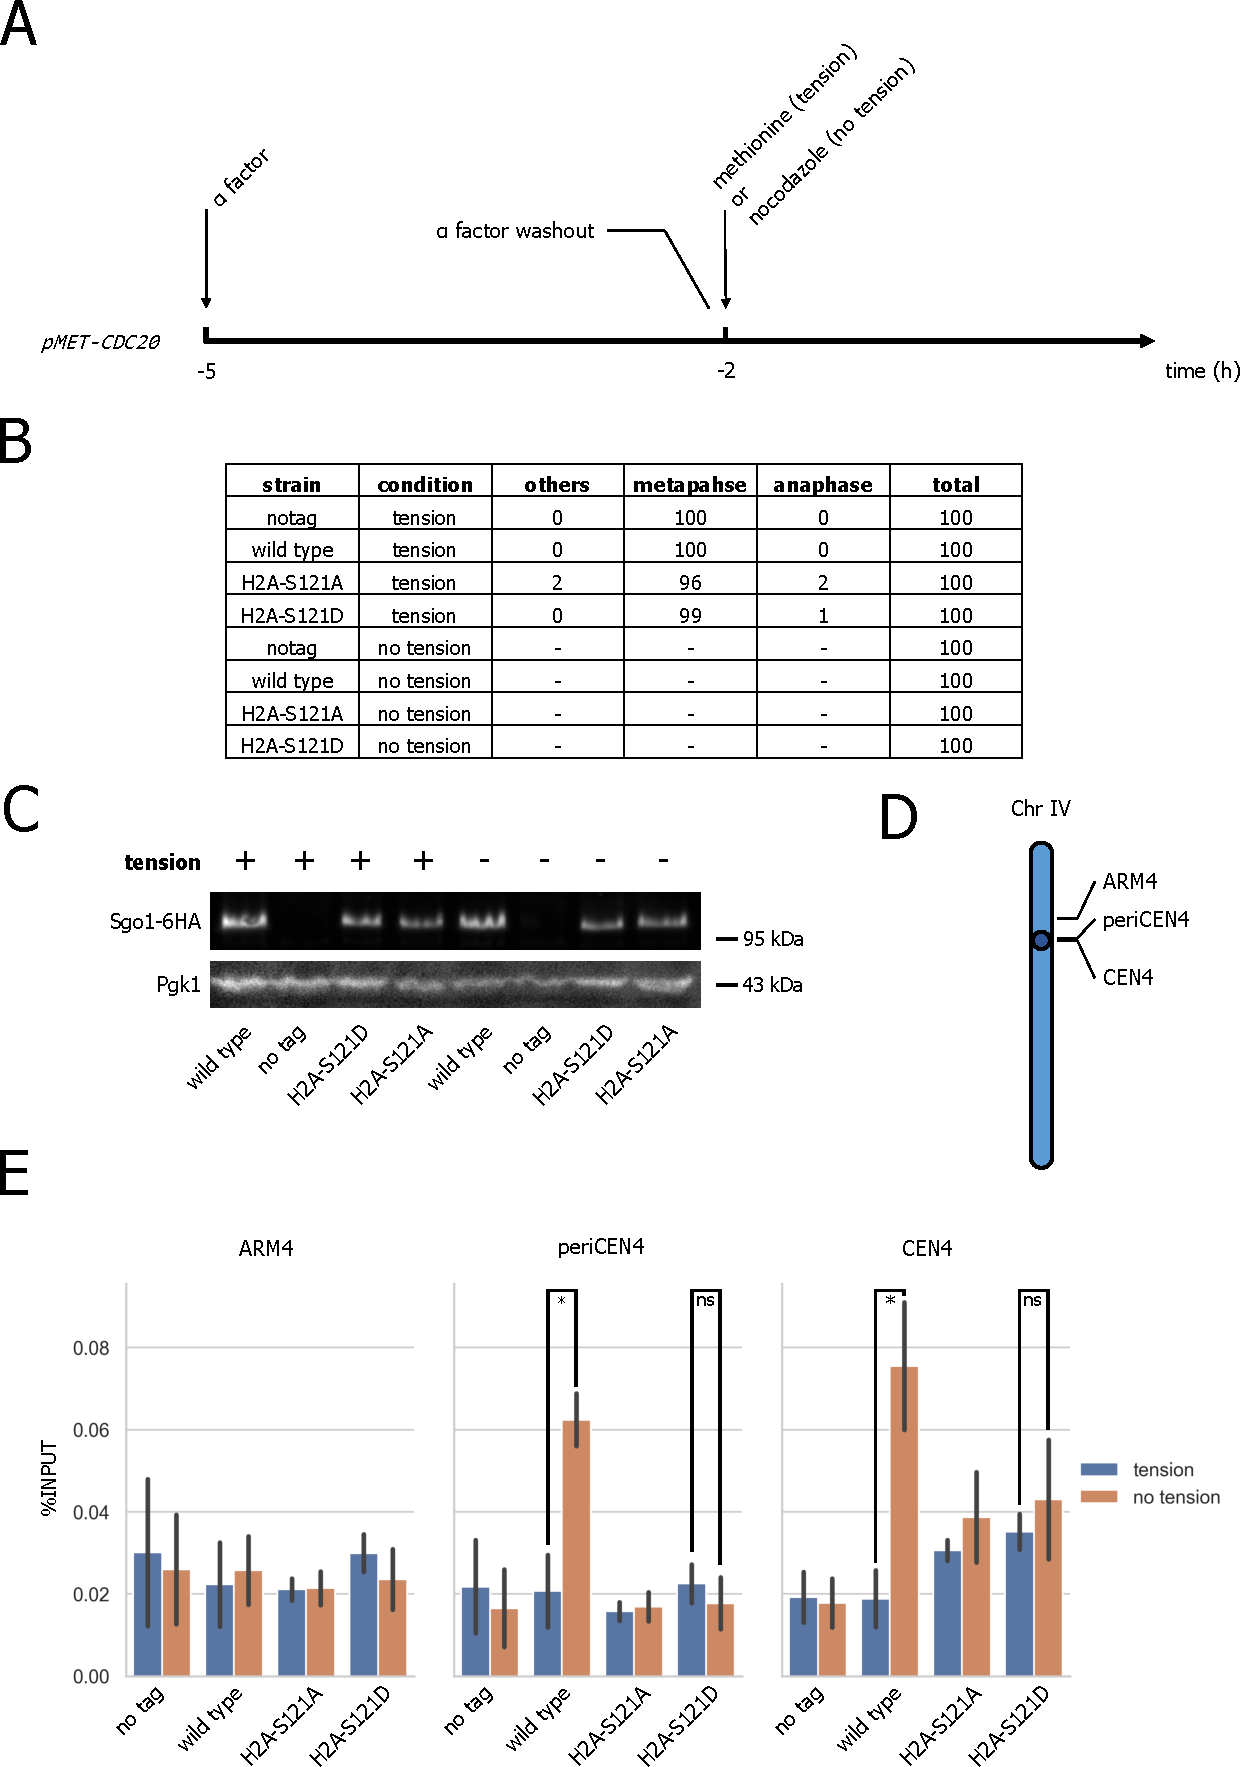
\includegraphics[width=0.9\textwidth]{chapter3/figures/Sgo1 in H2A mutants ChIP.pdf}
  \caption[Sgo1 association with chromatin remains low regardless of tension in H2A phospho-mimic mutant]{Sgo1 association with chromatin remains low regardless of tension in H2A phospho-mimic mutant. (A) Schematics of experimental procedures. (B) Spindle morphology count by tubulin IF. (C) Western blotting with anti-HA antibody to detect the expression level of Sgo1-6HA. Pgk1 was used as the loading control. (D) Schematics showing the locations of loci used for the ChIP-qPCR experiment. (E) Sgo1-6HA ChIP-qPCR on the chromosome arm, the peri-centromere and the core centromere of chromosome IV. The mean of 3 experimental repeats is shown, with the error bar representing standard error. The two-tailed independent t-test is used to calculate statistical significance. (*) P<0.05; (ns) not significant.}
  \label{fig:sgo1chiph2amutants}
\end{figure}

Due to the apparent contradiction with the previous result, I sought to validate the result with microscopy. Therefore, I constructed H2A mutants bearing genetic constructs for imaging, \textit{SGO1-EGFP MTW1-tdTomato}. Cells were imaged following the standard approach of synchronised G1 to metaphase live-cell imaging (Figure~\ref{fig:sgo1imagingh2amutants}A). Unlike wild type, where Sgo1-EGFP appeared as foci at least once in the cell cycle, both of the H2A phospho-mutants could only show Sgo1-EGFP as a 'cloud' signal (Figure~\ref{fig:sgo1imagingh2amutants}B and C). Again, this 'cloud' signal resembles what it looks like in wild type after the establishment of tension, judged by the separation of kinetochore foci. Western blotting showed similar Sgo1 expression levels in the three strains used, ruling out the possibility that the loss of Sgo1-EGFP foci is because of reduced protein abundance (Figure~\ref{fig:sgo1imagingh2amutants}D). Therefore, I concluded that Sgo1 cannot be concentrated at the peri-centromere in H2A phospho-mimic mutant. 

\begin{figure}[htbp]
  \centering
  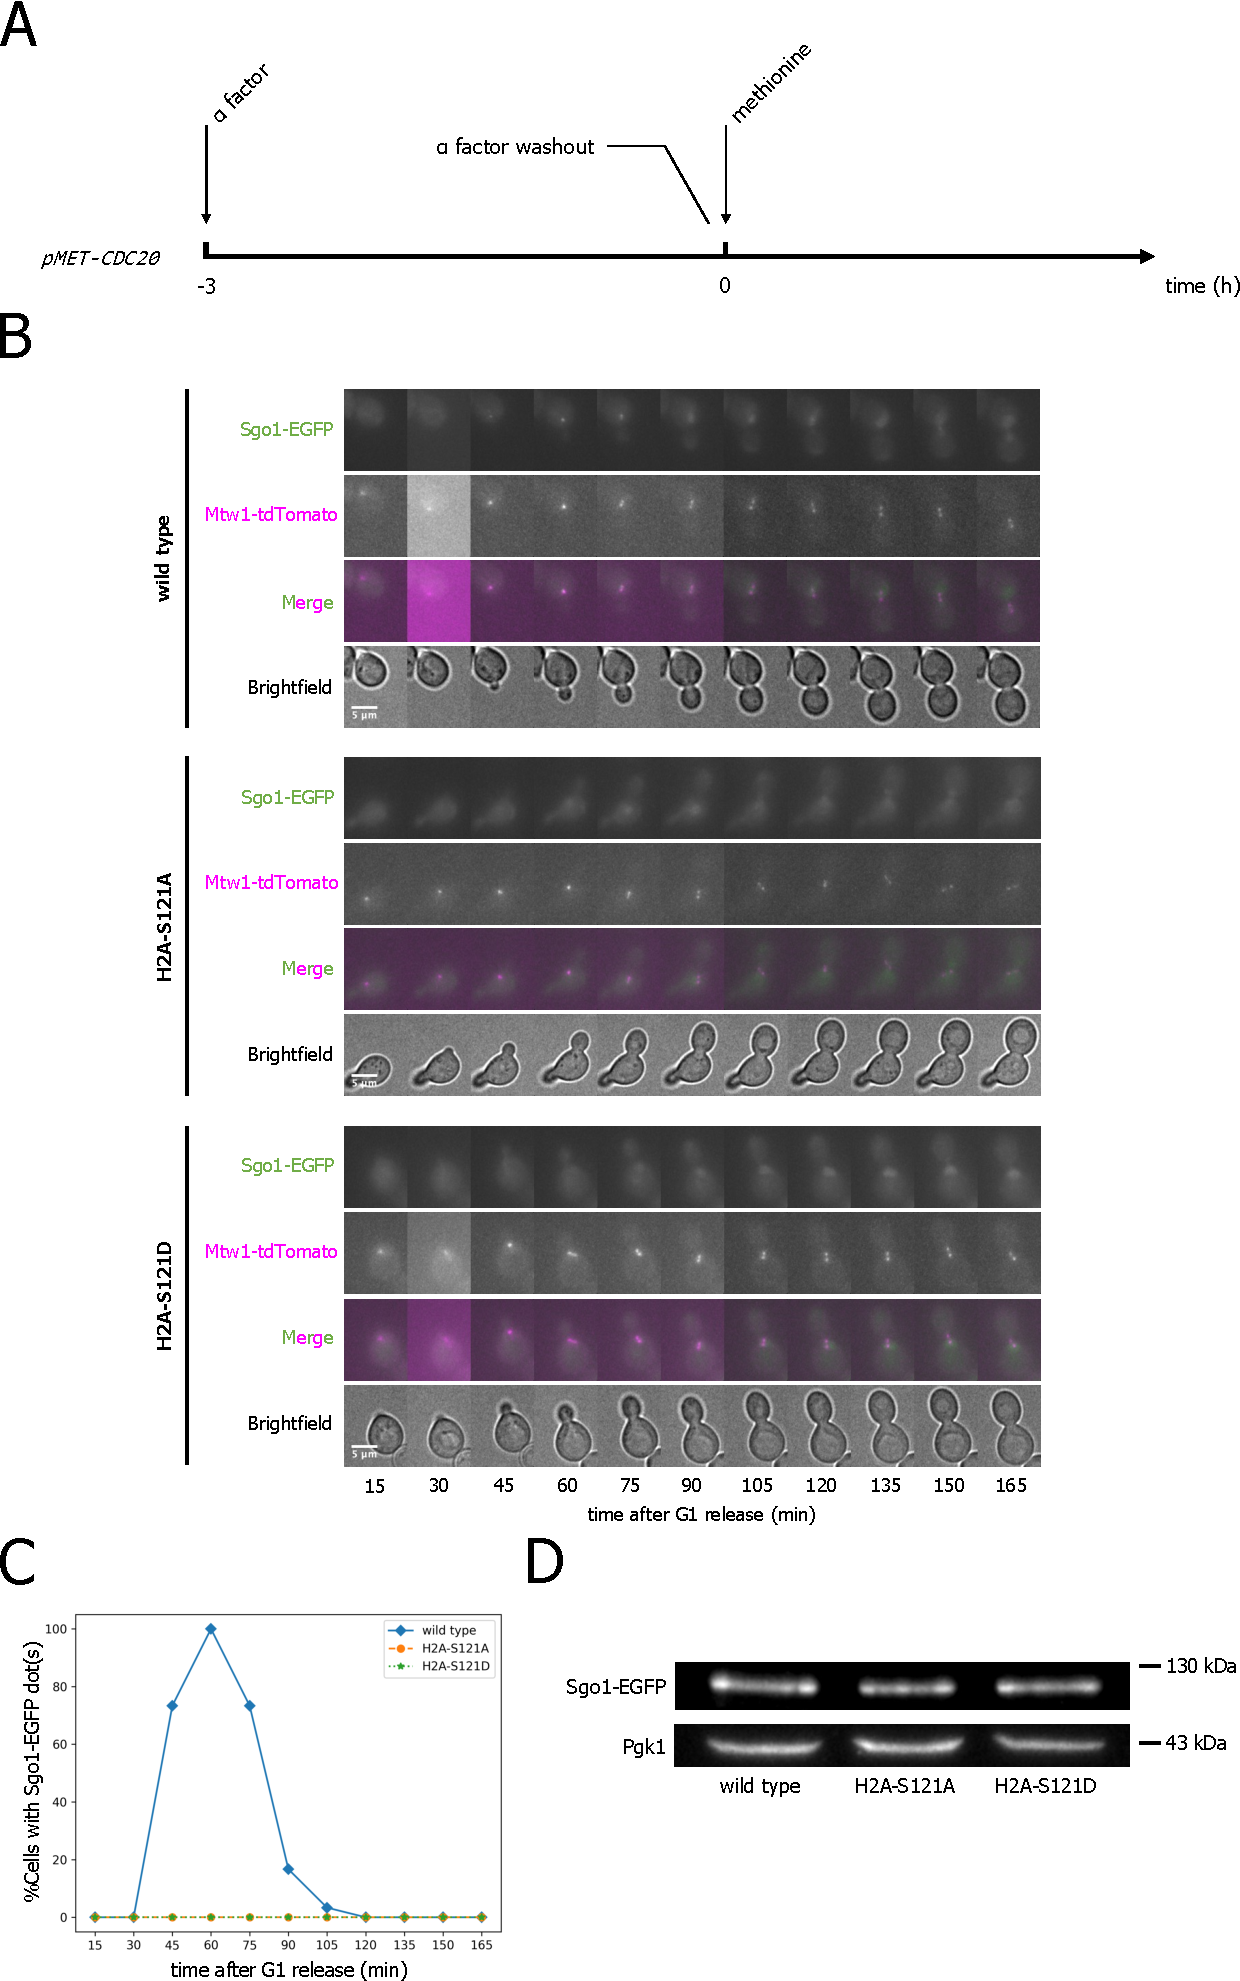
\includegraphics[width=0.9\textwidth]{chapter3/figures/Sgo1 in H2A mutants imaging.pdf}
  \caption[Sgo1 peri-centromere enrichment is abolished in H2A phospho-mimic mutant]{Sgo1 peri-centromere enrichment is abolished in H2A phospho-mimic mutant. (A) Schematics of experimental procedures. (B) Montages of representative time-lapse imaging. (C) N=30 cells for each strain were followed over time and quantified. The percentage of cells with Sgo1-EGFP foci was shown as a function of time. (D) Western blotting on cells arrested in metaphase without tension using anti-GFP antibody to detect the expression level of Sgo1-EGFP. Pgk1 was used as the loading control.}
  \label{fig:sgo1imagingh2amutants}
\end{figure}

\subsection{\textit{sgo1$\Delta$} suppresses the growth defect of PP1 temperature-sensitive mutants at their restrictive temperatures}

The working model predicts the existence of one or more phosphatases constantly de-phosphorylating H2A-pS121. We hypothesised PP1 to be one possible candidate. PP1 is a major serine/ threonine phosphatase ubiquitous in eukaryotes and regulates a large number of cellular processes, including SAC silencing and tension sensing \citep{Shi2009Serine/threonineStructure, Cannon2010FunctionCerevisiae, Pinsky2009ProteinYeast, Pinsky2006Glc7/proteinGlc7, London2012, Meadows2011SpindleMotors, Nijenhuis2014NegativeSignal, Rosenberg2011KNL1/Spc105Checkpoint, Liu2010RegulatedKinase, Posch2010Sds22Mitosis, Jin2013TheAttachment}. A functional PP1 enzyme usually consists of a catalytic subunit, which is highly conserved across species, and a regulatory subunit controlling the localisation, substrate specificity, or activity of the catalytic subunit or serves as the substrate itself. The recognition of the catalytic subunit is majorly through the RxVxF motif, and is often accompanied by an additional MyPhoNE or SILK motif \citep{Hendrickx2009DockingPhosphatase-1}. Budding yeast has a single gene encoding the catalytic subunit called \textit{GLC7} \citep{Cannon2010FunctionCerevisiae}. Consistent with its role in SAC silencing, inactivating Glc7 by using temperature-sensitive mutants results in prolonged metaphase arrest and therefore inviability \citep{Andrews2000TypeCerevisiae, MacKelvie1995ThePhosphatase}. 

I started by checking if \textit{SGO1} has genetic interaction with \textit{GLC7}. It has been shown that not allowing Sgo1 re-localisation upon tension by tethering Sgo1 to the kinetochore also arrests cells in metaphase \citep{Su2021SumoylationAnaphase}. If PP1 is the phosphatase that de-phosphorylates H2A-pS121, the growth defect from Glc7 inactivation could be partially attributed to impaired Sgo1 removal. Hence, depleting Sgo1 should be able to relieve it. To test this idea, I constructed double mutants of \textit{sgo1$\Delta$} and \textit{GLC7} temperature-sensitive alleles, either \textit{glc7-10} or \textit{glc7-12}, and carried out spot assay. As reported in previous research \citep{MacKelvie1995ThePhosphatase, Andrews2000TypeCerevisiae}, at their respective restrictive temperatures, 37 \si{\celsius} for \textit{glc7-10} and 34 \si{\celsius} for \textit{glc7-12}, both single mutants were inviable. However, when combined with \textit{sgo1$\Delta$} as double mutants, both strains showed a slight increase in viability (Figure~\ref{fig:growthassay}A), supporting the idea that PP1 is involved in Sgo1 re-localisation from the peri-centromere. 

To verify this result, I wanted to test if \textit{bub1$\Delta$K} mutant, which has unphosphorylated H2A and cannot localise its Sgo1, could phenocopy \textit{sgo1$\Delta$} in restoring the viability of \textit{GLC7} temperature-sensitive mutants. To our surprise, the double mutants indicated the same, if not less, viability compared to \textit{glc7-10} or \textit{glc7-12} single mutant (Figure~\ref{fig:growthassay}B). This finding argues against the hypothesis. However, it has been reported in humans that Bub1 kinase activity is required for cellular processes other than localising Sgo1 \citep{Tang2004, Nyati2015TheSignaling, Li2018TheReplication, Zhang2020FunctioningMitosis}. We reasoned that the loss of other functions of Bub1 kinase might outweigh the benefit of removing Sgo1 from the peri-centromere in the double mutants here. 

\begin{figure}[htbp]
  \centering
  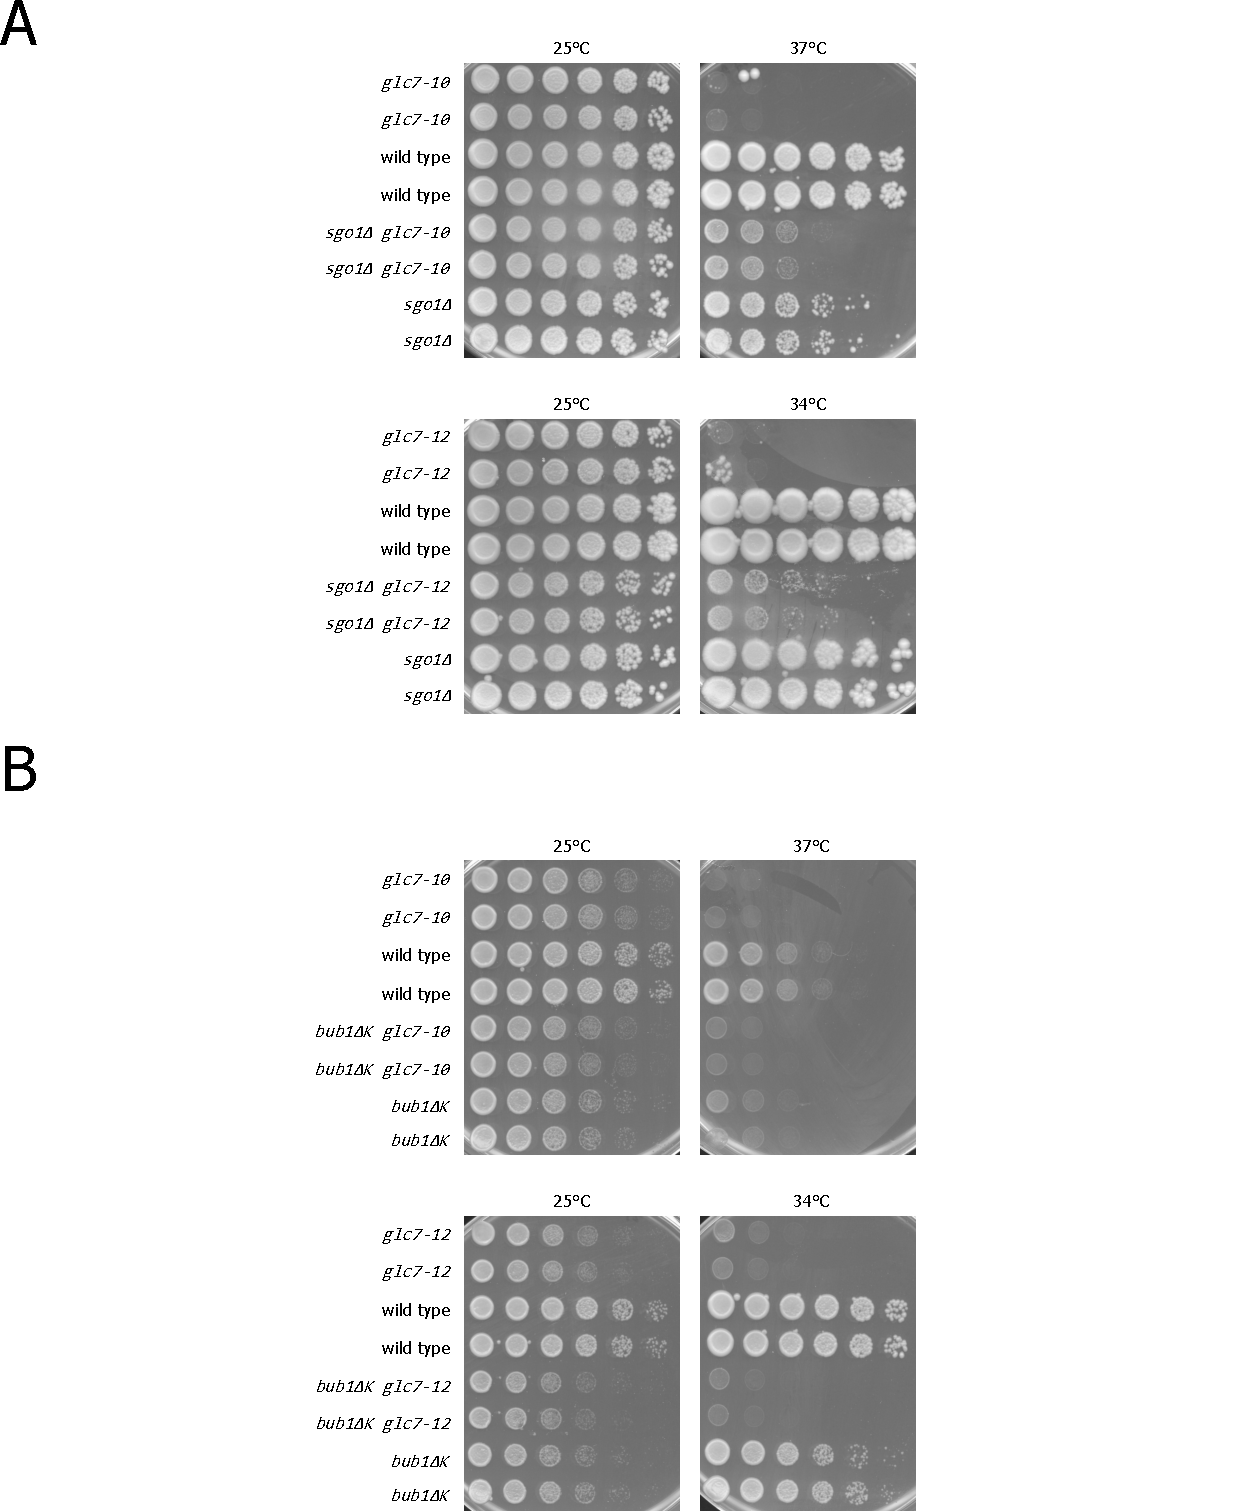
\includegraphics[width=0.9\textwidth]{chapter3/figures/glc7 mutants growth assaay.pdf}
  \caption[\textit{sgo1$\Delta$} but not \textit{bub1$\Delta$K} suppresses the temperature sensitivity of \textit{glc7-10} and \textit{glc7-12} mutant]{\textit{sgo1$\Delta$} but not \textit{bub1$\Delta$K} suppresses the temperature sensitivity of \textit{glc7-10} and \textit{glc7-12} mutant. (A) Serial dilutions of wild type, \textit{sgo1$\Delta$} and \textit{glc7-10} or \textit{glc7-12} single and double mutants spotted on rich medium at room or restrictive temperature. (B) Serial dilutions of wild type, \textit{bub1$\Delta$K} and \textit{glc7-10} or \textit{glc7-12} single and double mutants spotted on rich medium at room or restrictive temperature. The duplications represent technical repeats. }
  \label{fig:growthassay}
\end{figure}

\nomenclature{PP1}{Protein Phosphatase 1}

\subsection{PP1 is required for Sgo1 re-localization}

With the results from the spot assay, I wanted to study the localisation of Sgo1 upon Glc7 inactivation to test whether PP1 is required for Sgo1 removal from the peri-centromere. I first constructed the strain with genetic constructs for Sgo1 imaging (\textit{SGO1-EGFP MTW1-tdTomato pMET-CDC20}) and \textit{glc7-12}, whose restrictive temperature is lower than \textit{glc7-10} and thus might be more compatible with live-cell imaging. the standard G1 to metaphase arrest with tension imaging was conducted except that cells were shifted to 34 \si{\celsius} immediately after G1 release to inactivate PP1 (Figure~\ref{fig:sgo1glc712}A). 

In terms of the inter-kinetochore distance, wild type was similar as in the previous experiments, albeit escaped the arrest induced by Cdc20 depletion near the end of imaging, possibly due to the elevated temperature. Whereas in \textit{glc7-12}, it was stabilised at a much shorter distance, around 0.5 \si{\micro\metre}, over time (Figure~\ref{fig:sgo1glc712}B and C), consistent with the previous report that \textit{glc7-12} cells were arrested in metaphase with short spindles \citep{MacKelvie1995ThePhosphatase}. Interestingly, similar to some of other \textit{GLC7} mutants \citep{Black1995A1, Andrews2000TypeCerevisiae}, many \textit{glc7-12} cells showed elongated bud morphology. The elevated temperature reduced the imaging quality yet the Sgo1-EGFP foci remained distinguishable from the background. Strikingly, in contrast to wild type, Sgo1-EGFP was retained as foci till the end of the experiment in \textit{glc7-12}. Quantification showed that the percentage of \textit{glc7-12} having Sgo1-EGFP foci increased over time and reached nearly 100\% (Figure~\ref{fig:sgo1glc712}B and C), suggesting that Sgo1 cannot be de-localised from the peri-centromere without functional PP1. 

The shortened inter-kinetochore distance in \textit{glc7-12} raised the possibility that Sgo1 is not re-localised because of reduced tension. To test if enough tension was generated in \textit{glc7-12}, I sought to compare the inter-kinetochore distance at which Sgo1 is removed in wild type and the maximum that \textit{glc7-12} could reach. Technically, for individual wild type cell, I identified the first frame that Sgo1-EGFP foci disappeared and recorded its distance between Mtw1-tdTomato foci, which I referred to as wild type$_{removal}$; while for individual \textit{glc7-12} cell, I followed it over time and selected the longest distance its Mtw1-tdTomato foci ever separated, which I named as \textit{glc7-12}$_{maximum}$. As shown in Figure~\ref{fig:sgo1glc712}D, \textit{glc7-12}$_{maximum}$ was slightly larger than wild type$_{removal}$, indicating that \textit{glc7-12} had reached inter-kinetochore distances where Sgo1 is supposed to be de-localised. Therefore, I concluded that the retention of Sgo1 in \textit{glc7-12} cannot be simply explained by the reduced tension. Western blotting further confirmed that this retention is not due to an altered Sgo1-EGFP expression in \textit{glc7-12} (Figure~\ref{fig:sgo1glc712}E). 

\begin{figure}[htbp]
  \centering
  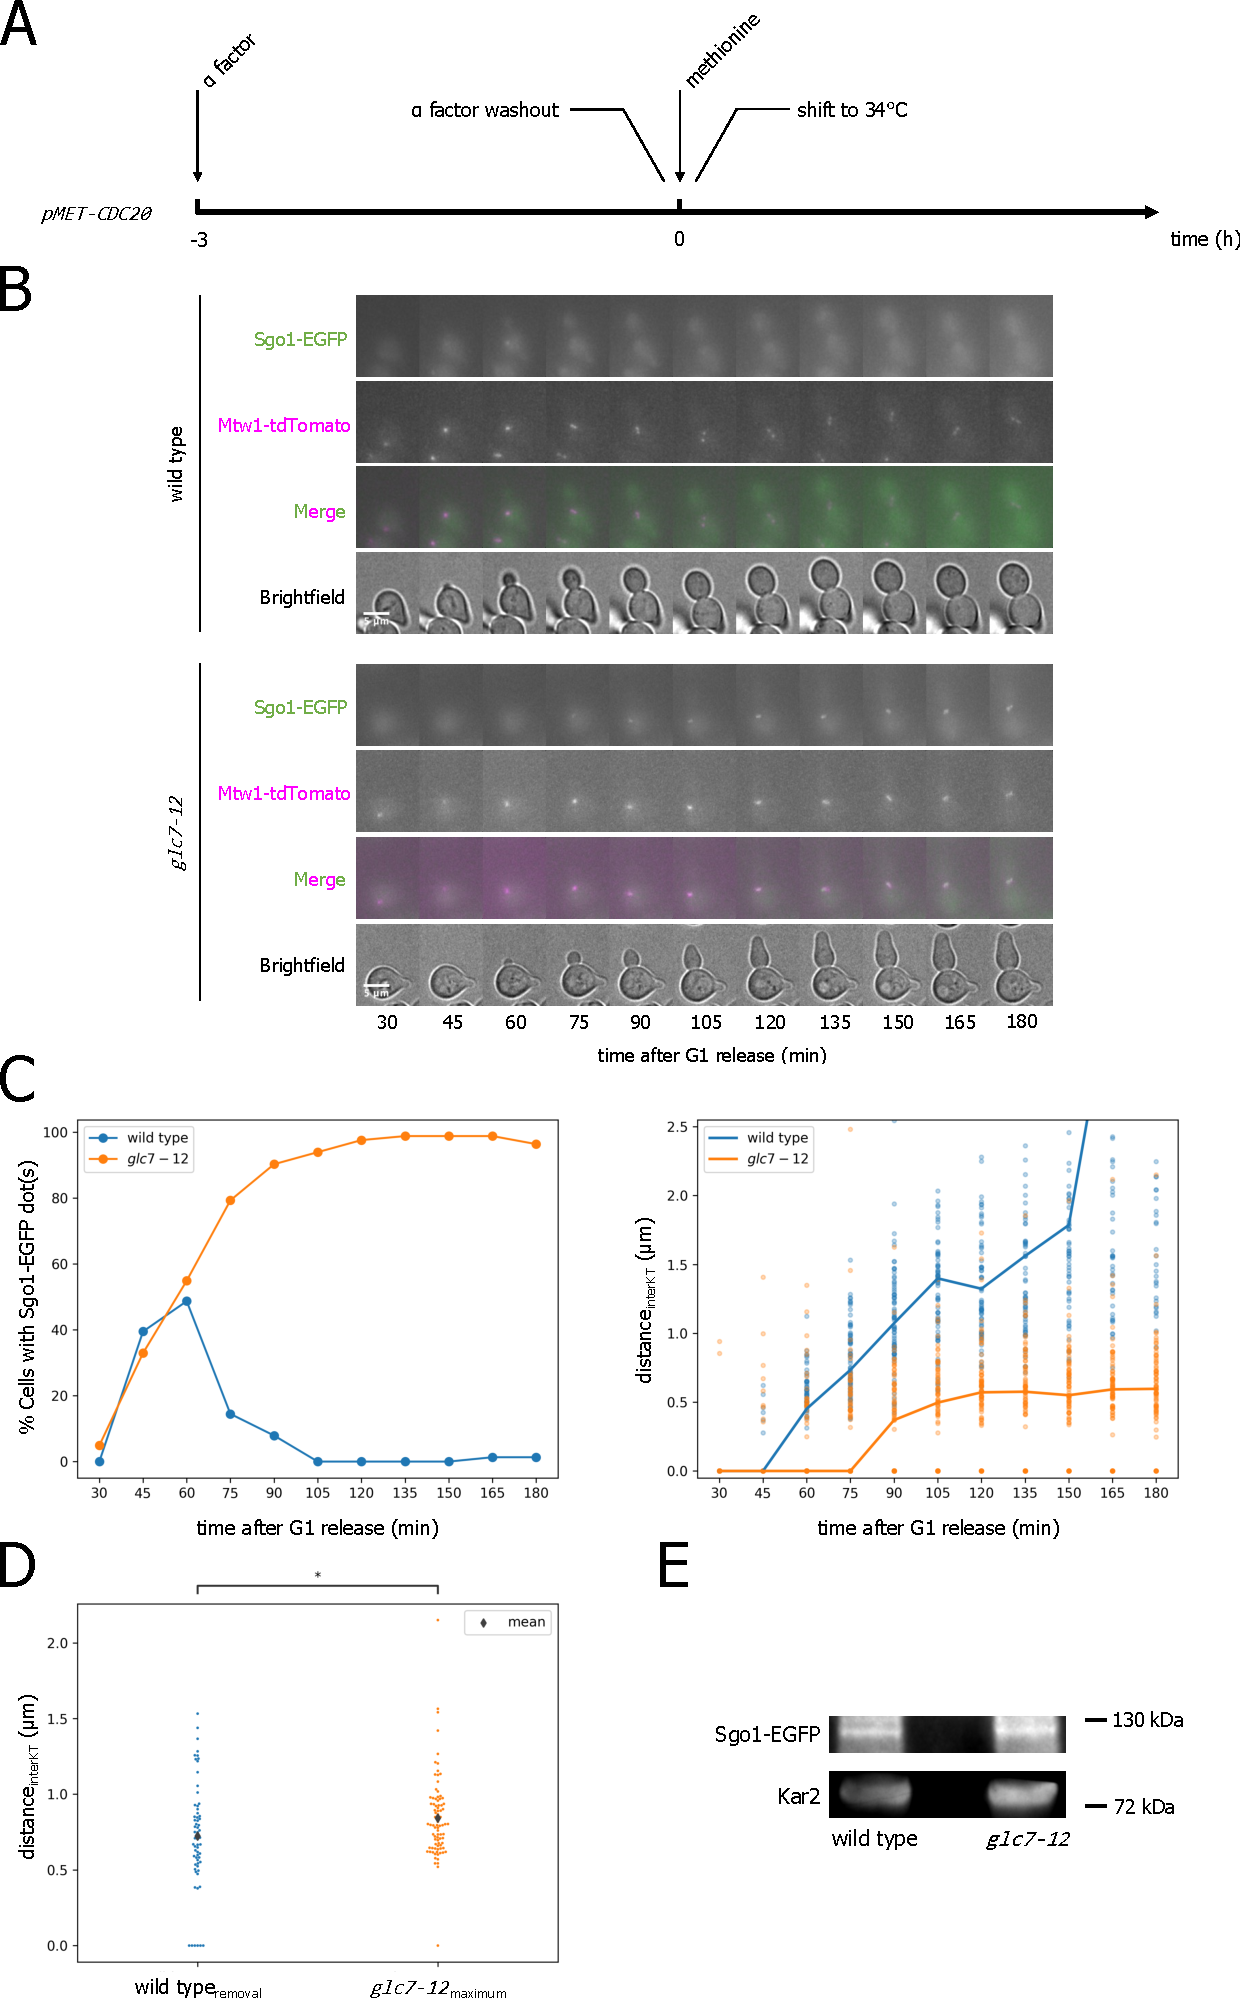
\includegraphics[width=0.9\textwidth]{chapter3/figures/Sgo1 glc7-12.pdf}
  \caption[Sgo1 is not de-localised from peri-centromere in \textit{glc7-12} at restrictive temperature]{Sgo1 is not de-localised from peri-centromere in \textit{glc7-12} at restrictive temperature. (A) Schematics of experimental procedures. (B) Montages of representative time-lapse imaging. (C) N=100 cells for each strain were followed over time and quantified. Top panel: the percentage of cells with Sgo1-EGFP foci was shown as a function of time. Bottom panel: median inter-kinetochore distance as a function of time. Individual data points are shown as dots. (D) Comparison between the inter-kinetochore distance at which Sgo1 is removed in wild type (wild type$_{removal}$) and the maximum that \textit{glc7-12} could reach (\textit{glc7-12}$_{maximum}$). The two-tailed independent t-test was used to calculate statistical significance. (*) P<0.05 (E) Western blotting on cells arrested in metaphase without tension using anti-GFP antibody to detect the expression level of Sgo1-EGFP. Kar2 was used as the loading control.}
  \label{fig:sgo1glc712}
\end{figure}

To verify the result, I repeated the experiment in \textit{glc7-10} background (Figure~\ref{fig:sgo1glc710}A). Consistently, Sgo1-EGFP was maintained as foci within the scope of the experiment (Figure~\ref{fig:sgo1glc710}B), supporting the conclusion that PP1 is required for Sgo1 re-localisation. Notably, this experiment's imaging quality was better compared to the one for \textit{glc7-12}. This is unexpected as it was conducted at an even higher temperature. I suspect it might be related to the fact there is immersion oil optimised for imaging at 37 \si{\celsius} but not 34 \si{\celsius}. 

\begin{figure}[htbp]
  \centering
  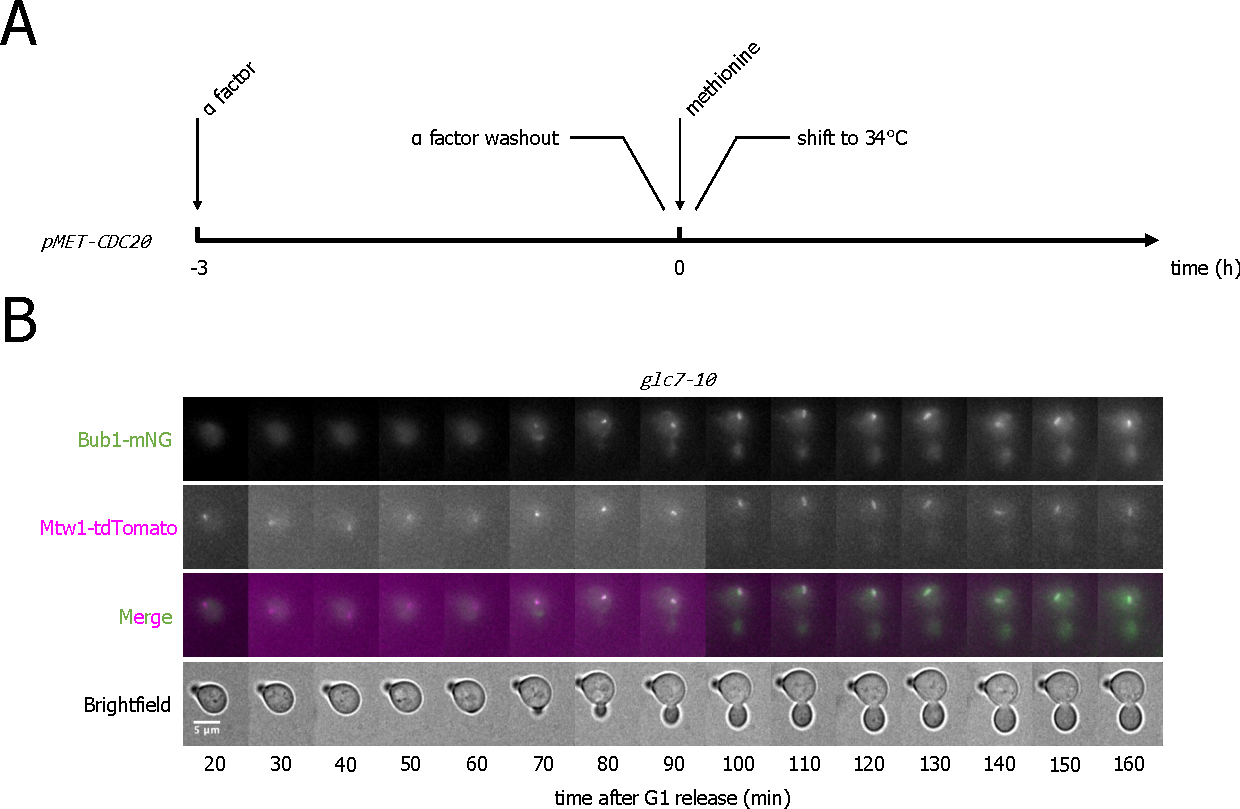
\includegraphics[width=0.9\textwidth]{chapter3/figures/Sgo1 glc7-10.pdf}
  \caption[Sgo1 is not de-localised from peri-centromere in \textit{glc7-10} at restrictive temperature]{Sgo1 is not de-localised from peri-centromere in \textit{glc7-10} at restrictive temperature. (A) Schematics of experimental procedures. (B) Montages of representative time-lapse imaging.}
  \label{fig:sgo1glc710}
\end{figure}

\subsection{PP1-inactivation-caused retention of Sgo1 depends on Bub1}

Next, we wondered whether PP1 is the phosphatase counteracting Bub1 in terms of localising Sgo1. If so, we expected that Sgo1 localisation should be maintained in the absence of both Bub1 and PP1 (Figure~\ref{fig:bub1aidglc712}B). To test this idea, I repeated the 
Bub1 depletion experiment of Figure~\ref{fig:bub1aid} but in the \textit{glc7-12} genetic background. Cells were synchronised in G1 at RT and released to media containing methionine and nocodazole at the restrictive temperature for a metaphase arrest with inactivated PP1 and no tension. NAA was then added to deplete Bub1. Microscopy was used to monitor the localisation of Sgo1 (Figure~\ref{fig:bub1aidglc712}A). Cells showed abnormal bud morphology, indicating successful inactivation of PP1. Unlike the control, Sgo1-EGFP quickly lost its foci signal in the +NAA group with similar dynamics to the previous experiment in Figure~\ref{fig:bub1aid} (Figure~\ref{fig:bub1aidglc712}C and D), suggesting PP1 does not directly counteract Bub1 to de-localise Sgo1. The depletion of Bub1 was not checked in this experiment because Sgo1 peri-centromere localisation was abolished when NAA was added, indicating that Bub1 was depleted as expected. 

\begin{figure}[htbp]
  \centering
  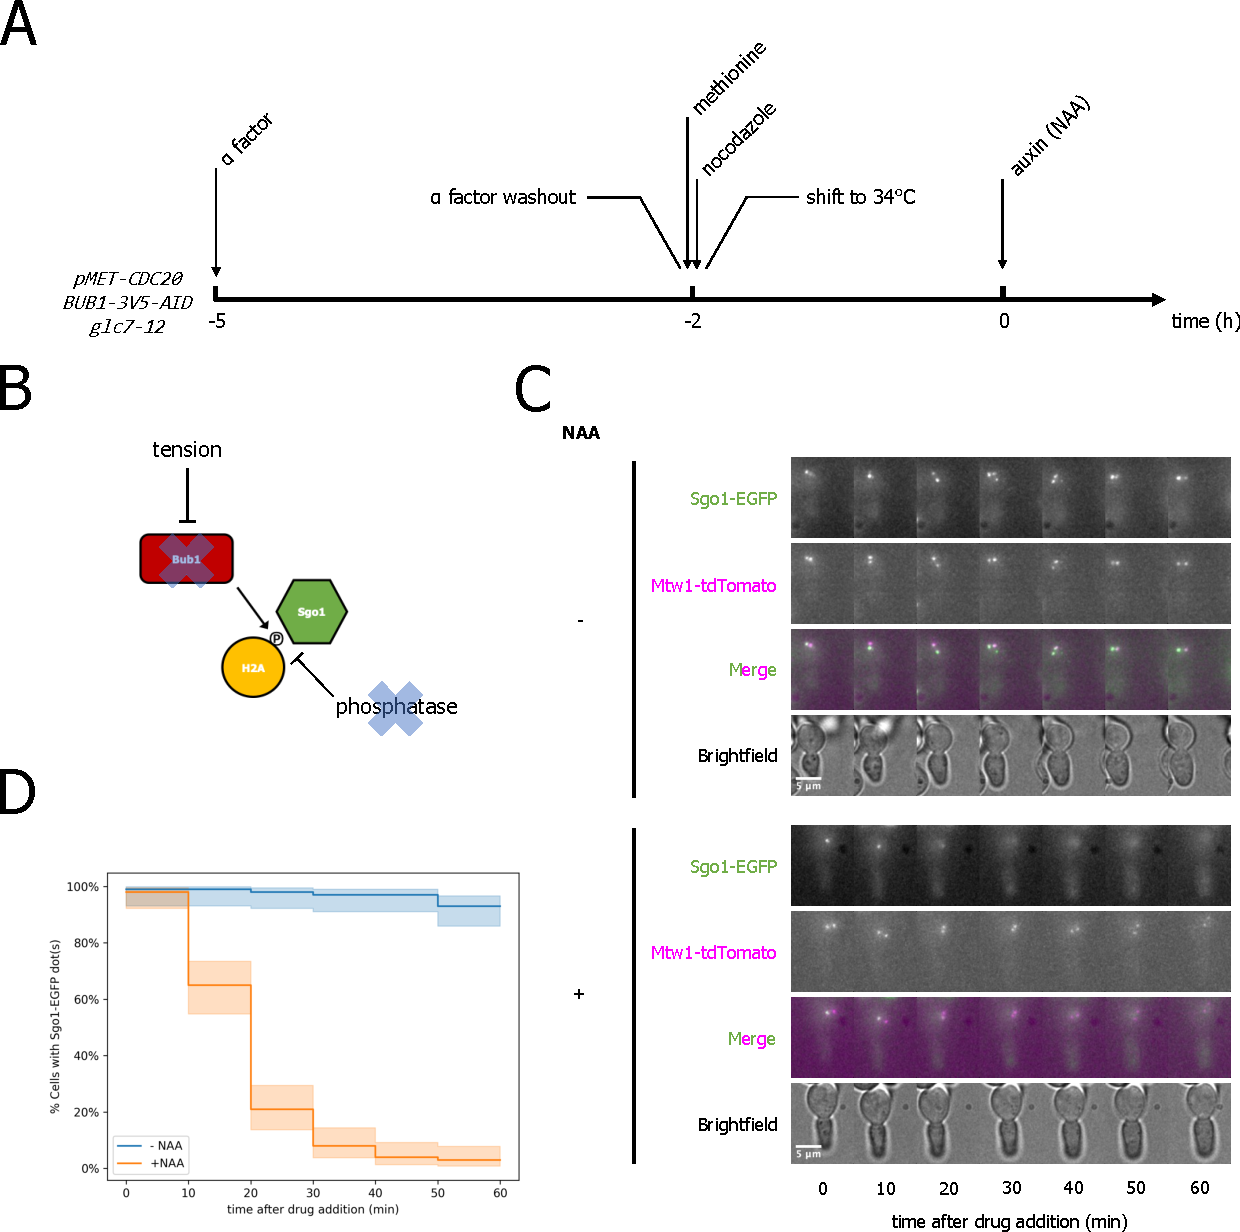
\includegraphics[width=0.9\textwidth]{chapter3/figures/Bub1-AID glc7-12.pdf}
  \caption[PP1 inactivation does not rescue the prompt de-localisation of Sgo1 upon Bub1 depletion in the absence of tension.]{PP1 inactivation does not rescue the prompt de-localisation of Sgo1 upon Bub1 depletion in the absence of tension. (A) Schematics of experimental procedures. (B) Schematics of experimental concept. (C) Montages of representative time-lapse imaging. (D) Survival analysis of the duration of focused Sgo1-EGFP signal. N=30 cells for each strain were followed over time and quantified for the duration of the Sgo1-EGFP signal being focused. Solid lines are Kaplan-Meier survival estimates. The shaded area in the same colour is the 95\% confidence limit of the estimate.}
  \label{fig:bub1aidglc712}
\end{figure}

\subsection{PP1 is required for Bub1 re-localization}

 It has been reported in budding yeast that PP1 could de-phosphorylate the MELT motifs of Spc105, the ortholog of human KNL1, which are important for Bub1 kinetochore localisation \citep{London2012, Roy2019}. We reasoned that the observation that Sgo1 cannot be de-localised upon PP1 inactivation could be due to the retention of Bub1 at the kinetochore in the same condition. To verify this idea, I wanted to study the localisation of Bub1 when PP1 is inactivated. A synchronised G1 to metaphase live-cell imaging at the restrictive temperature of \textit{glc7-12} was performed (Figure~\ref{fig:bub1glc712}A). In wild type, the dynamics of kinetochore-localised Bub1-mNG was as previously described, which was largely reduced at 75 \si{\minute} after G1 release, corresponding to the separation of Mtw1-tdTomato foci. As expected, the drop was not observed in \textit{glc7-12} (Figure~\ref{fig:bub1glc712}B and C), indicating Bub1 de-localisation from the kinetochore upon tension is impaired when PP1 is inactivated. Consistent with the previous experiment, the stabilised inter-kinetochore distance in \textit{glc7-12} was about 0.5 \si{\micro\metre}. Western blotting indicated reduced Bub1 expression in \textit{glc7-12} compared to wild type, probably due to cell death and poorer cell cycle synchronisation. However, it still ruled out the possibility that the increased kinetochore Bub1-mNG fluorescence intensity was because of elevated Bub1 protein level in \textit{glc7-12}. Therefore, combined with the result in the previous section, I concluded that PP1 is required for Sgo1 re-localization due to its role in de-localising Bub1 from the kinetochore. 

\begin{figure}[htbp]
  \centering
  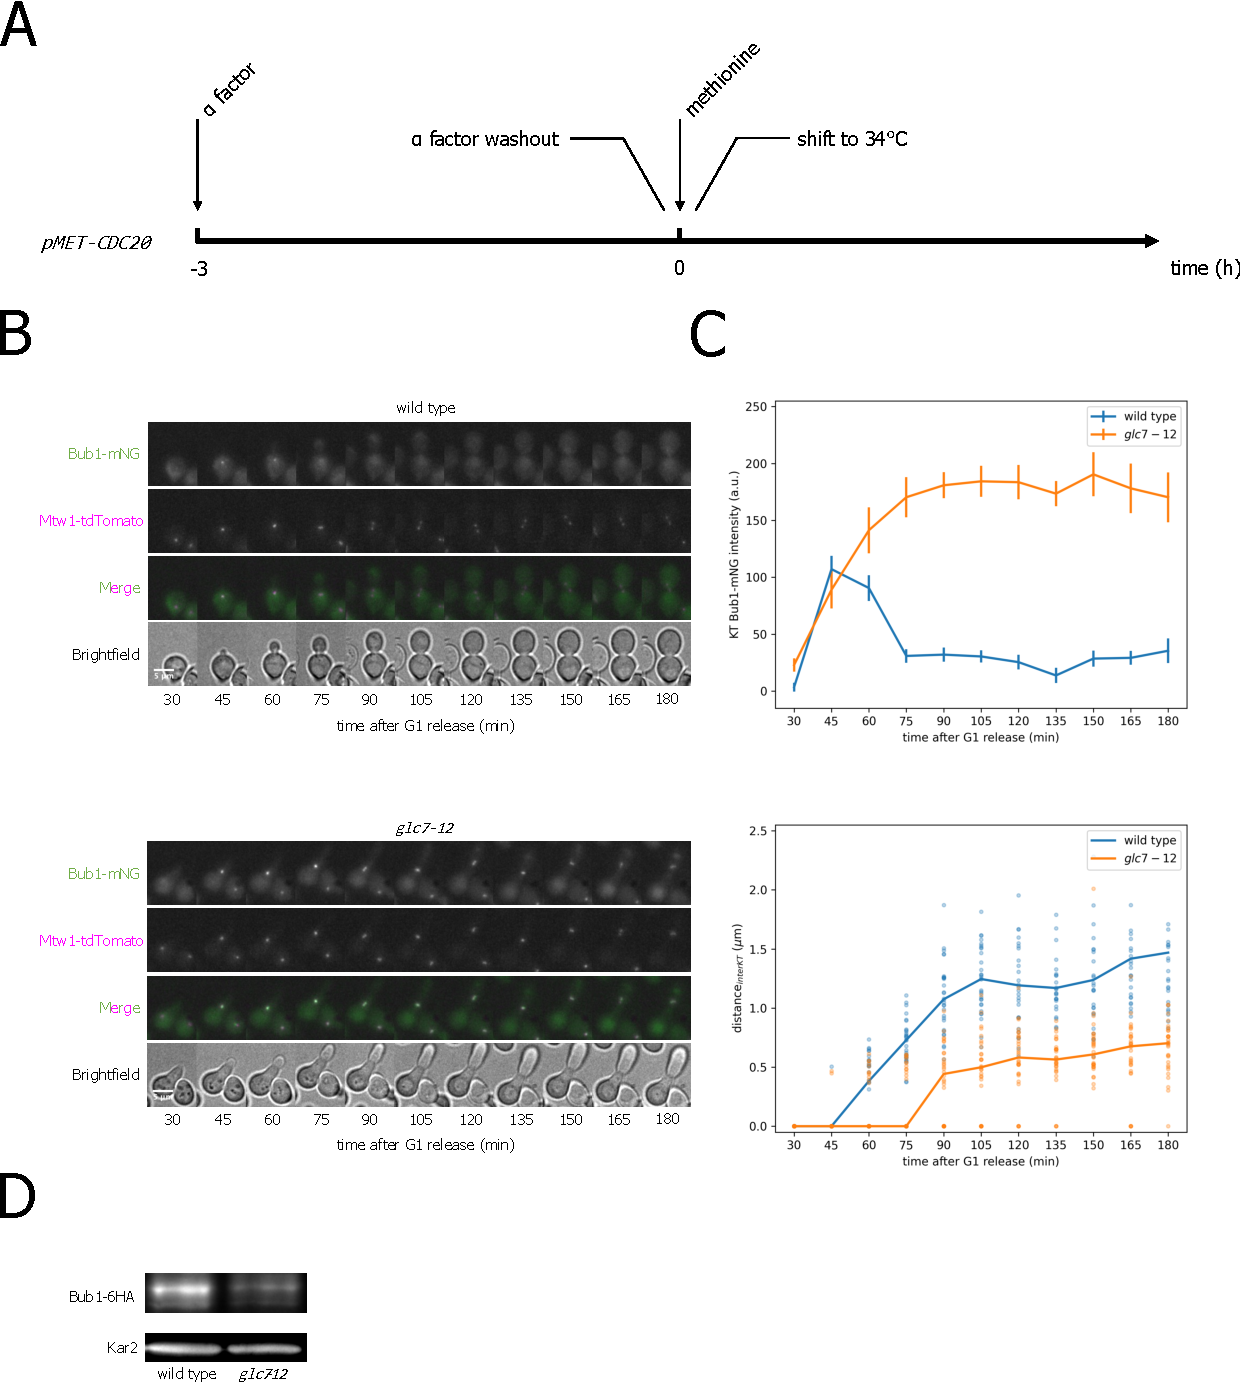
\includegraphics[width=0.9\textwidth]{chapter3/figures/Bub1 glc7-12.pdf}
  \caption[Kinetochore-localised Bub1 is maintained upon PP1 inactivation]{Kinetochore-localised Bub1 is maintained upon PP1 inactivation. (A) Schematics of experimental procedures. (B) Montages of representative time-lapse imaging. (C) N=30 cells for each strain were followed over time and quantified for kinetochore Bub1-mNG fluorescence intensity and inter-kinetochore distance. Top panel: mean fluorescence intensity of Bub1-mNG at the kinetochore as a function of time. The error bar represents the standard error. Bottom panel: Median inter-kinetochore distance as a function of time. Individual data points are shown as dots. (D) Western blotting on cells arrested in metaphase without tension using anti-HA antibody to detect the expression level of Bub1-6HA. Kar2 was used as the loading control.}
  \label{fig:bub1glc712}
\end{figure}

\subsection{Putative PP1 binding motifs of Sgo1 are not required for Sgo1 re-localization}

Interestingly, the budding yeast Sgo1 protein sequence contains the consensus PP1 recognition motif RxVxF and the assisting motif SILK, making it a possible regulatory subunit of PP1 (Figure~\ref{fig:sgo1phosphomutant}A). Given the necessity of PP1 in re-localising Sgo1, we hypothesised that the putative interaction between Sgo1 and PP1 could be the key. To test it, we mutated each or both of the motifs and conducted our standard synchronised G1 to metaphase live-cell imaging (Figure~\ref{fig:sgo1phosphomutant}B). Unexpectedly, in all three mutants, the time Sgo1-EGFP spent as foci were not significantly different from wild type (Figure~\ref{fig:sgo1phosphomutant}C), suggesting these motifs are not required for Sgo1 re-localisation. I further tested the functionality of Sgo1 in the mutants by measuring their benomyl sensitivity. In budding yeast, abnormality in SAC or chromosome segregation does not lead to severe growth defects in an undisturbed cell cycle. However, when challenged by the microtubule de-polymerising drug benomyl, it dramatically reduces the viability. As shown in Figure~\ref{fig:sgo1phosphomutant}D, the negative control \textit{sgo1$\Delta$} showed increased sensitivity to benomyl compared to wild type, representing the loss of Sgo1 functions in mitotic chromosome segregation. On the contrary, the mutants did not show an observable reduction in viability in the presence of benomyl, suggesting Sgo1 functions are intact in those strains. Due to the fact that all the mutants' Sgo1 was tagged by EGFP, I added an additional control \textit{SGO1-EGFP} to test if tagging EGFP itself can cause any change in Sgo1 functions. The similar sensitivity to benomyl between \textit{SGO1-EGFP} and wild type suggested a negative answer to the question. Therefore, I concluded that neither timely re-localisation nor the function of Sgo1 requires its putative PP1 binding sites. 

\begin{figure}[htbp]
  \centering
  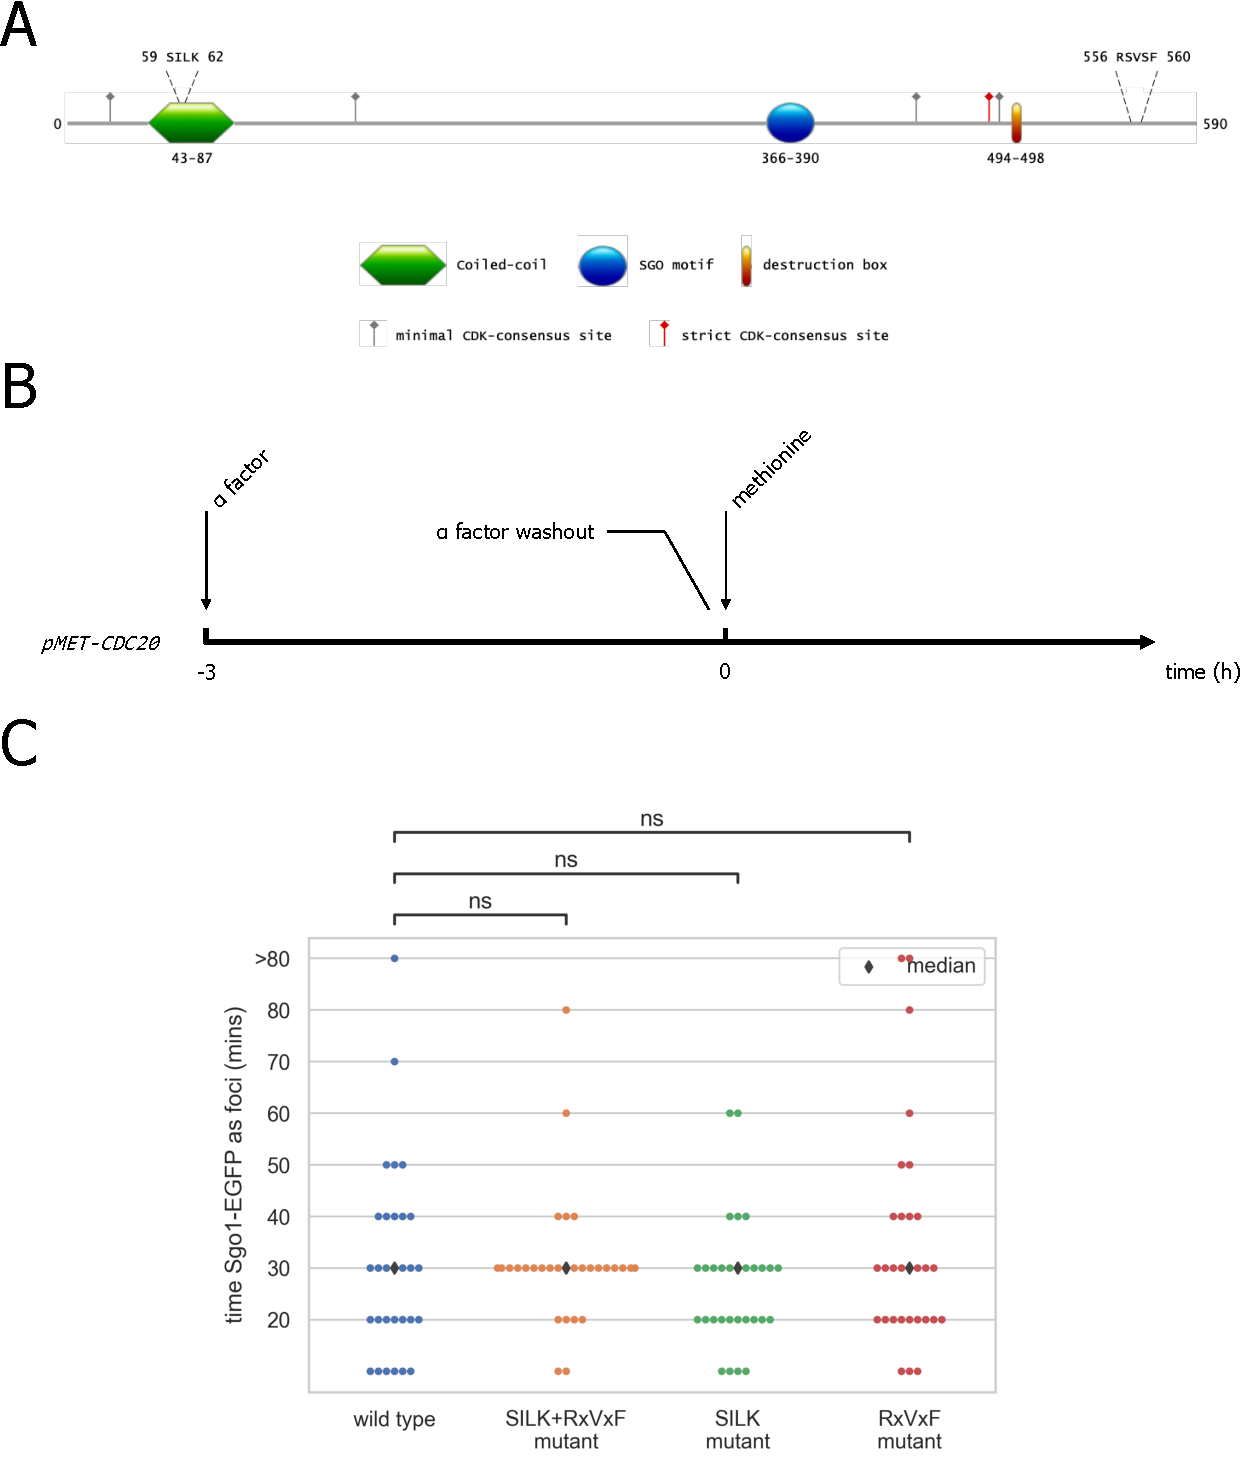
\includegraphics[width=0.9\textwidth]{chapter3/figures/Sgo1 putative PP1 binding mutants.pdf}
  \caption[Neither timely re-localisation nor the function of Sgo1 requires its putative PP1 binding sites]{Neither timely re-localisation nor the function of Sgo1 requires its putative PP1 binding sites. (A) Linear schematics of budding yeast Sgo1 protein. Putative PP1 binding motifs SILK and RSVSF are located at amino acid positions 59-62 and 556-560, respectively. (B) Schematics of the imaging experiment. (C) Quantification of the time of Sgo1-EGFP signal being visualised as foci. The two-tailed independent t-test was used to calculate statistical significance. (*) P<0.05; (ns) not significant. (D) Spot assay testing the benomyl sensitivity of the strains. Five-fold serial dilutions of indicated strains spotted on rich medium with 0 or 10 \si{\micro\gram/\milli\litre} benomyl.}
  \label{fig:sgo1phosphomutant}
\end{figure}

\subsection{PP2A-Rts1 might regulate Sgo1 phosphorylation}

Another attempt to identify the phosphatase involved in the re-localisation of Sgo1 focused on its interacting phosphatase PP2A-Rts1. \cite{Nerusheva2014} showed by ChIP-qPCR that deleting \textit{RTS1} or abolishing Sgo1-PP2A interaction led to an increased association of Sgo1 with the peri-centromeric chromatin in the absence of tension but not upon tension, leaving PP2A as an interesting candidate phosphatase for Sgo1 de-localisation remain to be elucidated. 

PP2A belongs to the type 2 protein phosphatase, PP2, the other phospho-protein phosphatase regulating cellular metabolism than PP1 \citep{Ingebritsen1983ProteinRegulation}. Highly conserved across species, it is demonstrated important in a large number of cellular processes including cell cycle regulation \citep{Janssens2001ProteinSignalling}. Interestingly, despite being one of the most abundant proteins in a cell, accounting for 1\% of total cellular proteins in some cases, PP2A possesses excellent substrate specificity and fine-tuned spatiotemporal regulation \citep{Shi2009Serine/threonineStructure}. This is because of its complicated regulatory mechanism. PP2A core enzyme is composed of a scaffold subunit (A subunit) and a catalytic subunit (C subunit). The core enzyme can interact with one of the various regulatory subunits (B subunit), which targets the substrates specifically, to form the holoenzyme. Four families of regulatory subunit have been identified, namely B (B55), B' (B56), B'' and B''', with each one further having several isoforms \citep{Shi2009Serine/threonineStructure}. In budding yeast, the picture is less complex. There are only two regulatory subunits, Cdc55 and Rts1, corresponding to B and B', respectively \citep{Zhao1997SaccharomycesFunctions}. 

Consistent with PP2A's delicate regulation mechanism, shugoshins specifically interact with the PP2A-B' holoenzyme \citep{Kitajima2006a, Riedel2006, Tang2006a}. Structural data suggest that two human Sgo1 proteins form a dimmer and bind the B' and C subunit of one PP2A holoenzyme through the conserved coiled-coil domain \citep{Xu2009StructureInteraction}. Mutations of the expected contact residues in budding yeast are sufficient to abolish its Sgo1-PP2A interaction, suggesting that this structure is likely to be conserved (Figure~\ref{fig:sgo1phosphorts1d}A). A recent study indicated the existence of further interacting site(s) on Sgo1 with the conserved binding pocket of PP2A-B' \citep{Ueki2021AMitosis}. 

PP2A-B' acts as the effector of many of the shugoshins' functions. It is well established that this interaction is essential for cohesion protection in meiosis I through localised de-phosphorylation of the meiosis-specific kleisin subunit, Rec8, of cohesin \citep{Marston2004a, Kitajima2004a, Katis2004, Rabitsch2004TwoII, Rattani2013Sgol2Oocytes, Llano2008Shugoshin-2Mice, Lee2008} and vertebrate mitosis by counteracting the prophase pathway \citep{Shintomi2009ReleasingSgo1, Rivera2009ShugoshinExtracts, Orth2011ShugoshinMad2, Huang2007, Tang2006a, Tanno2010, McGuinness2005ShugoshinCells, Kitajima2005, Salic2004VertebrateMitosis}. Although there exists conflicting data \citep{Verzijlbergen2014, Eshleman2014}, the bi-orientation promoting function of shugoshins has been reported to require interaction with PP2A-B'\citep{Peplowska2014, Rivera2012}. The interaction has also been indicated involved in spindle checkpoint silencing \citep{Rattani2013Sgol2Oocytes}. 

The commitment to investigating PP2A-Rts1 was decided before the re-establishment of the importance of H2A-pS121 in Sgo1 tension-dependent re-localisation. Instead, we were interested in the hypothesis that Sgo1 post-translational modifications could be the key to its localisation and that PP2A-Rts1 might regulate them. It is derived from the fact that shugoshin phosphorylation has been reported in multiple species \citep{Llano2008Shugoshin-2Mice, Tanno2010, Rattani2013Sgol2Oocytes, Pouwels2007ShugoshinPlk1, Kawashima2007, Lee2014RegulationPhosphorylation, Liu2013, Liu2013a, Clarke2005, Resnick2006INCENPDrosophila, Nogueira2014, Yahya2020} with a few cases affecting its localisation. In humans, CDK phosphorylates Sgo1 at T346 and enables the interaction with cohesin, targeting Sgo1 to the inner centromere. Tension-dependent dephosphorylation of this site then abolishes the interaction and liberates Sgo1 for the association with kinetochore-proximal H2A-pT120, leading to its re-localisation \citep{Liu2013, Liu2013a}. There are also studies reporting CPC-dependent phosphorylation of human Sgo1 affects its localisation \citep{Pouwels2007ShugoshinPlk1, Lee2014RegulationPhosphorylation}. The localisation of \textit{Drosophila} shugoshin ortholog MEI-S332 seems to be dominantly under phospho-regulation. Its centromeric localisation in both mitosis and meiosis requires the phosphorylation by CPC \citep{Resnick2006INCENPDrosophila, Nogueira2014}, whereas the removal during the metaphase-anaphase transition depends on the direct binding and phosphorylation by POLO kinase \citep{Clarke2005}. Despite that the functions have not been elucidated, Sgo1 has been shown to be phosphorylated in budding yeast \citep{Yahya2020, Barton2019MechanismsCerevisiae}. 

To test the hypothesis, we started by asking whether the phosphorylation status of Sgo1 is altered upon \textit{RTS1} deletion. Sgo1-6HIS-3FLAG was immuno-precipitated from wild type or \textit{rts1$\Delta$}. Due to the Sgo1 expression level being cell-cycle-dependent, cells were arrested in metaphase without tension using benomyl for a higher yield. Immuno-precipitated peptides were then digested by trypsin, subjected to phospho-enrichment and identified by MS (Figure~\ref{fig:sgo1phosphorts1d}). Similar to the previous Sgo1 IP-MS done in the lab, amino acid 185-276 could not be revealed in the output data \citep{Barton2019MechanismsCerevisiae}. This is because this region lacks trypsin recognition residue lysine and hence cannot be digested to lengths short enough for MS analysis. Within the two repeats conducted, peptides of amino acid 143-155, 418-433, 475-485 and 484-494 were consistently detected to be phosphorylated. Relative intensities of phosphorylated peptides between wild type and \textit{rts1$\Delta$} were compared (Figure~\ref{fig:sgo1phosphorts1d}C). Phosphorylated peptides showing the same direction of enrichment in both repeats were considered genuine. The analysis indicated that the Sgo1 peptide of amino acid 418-433 showed increased phosphorylation while the peptide of amino acid 484-494 showed reduced phosphorylation in \textit{rts1$\Delta$}. Due to the fact that mass spectrometers can only detect the number of phosphorylation sites in a peptide but not the exact location, all phosphorylatable residues, serine, threonine and tyrosine, in the identified peptide have the potential to be regulated. Therefore, I concluded that PP2A-Rts1 could down-regulate the phosphorylation of Sgo1 at S421, S423 and S426 whereas up-regulate that at S486, S487, T493 and S496. 

\begin{figure}[htbp]
  \centering
  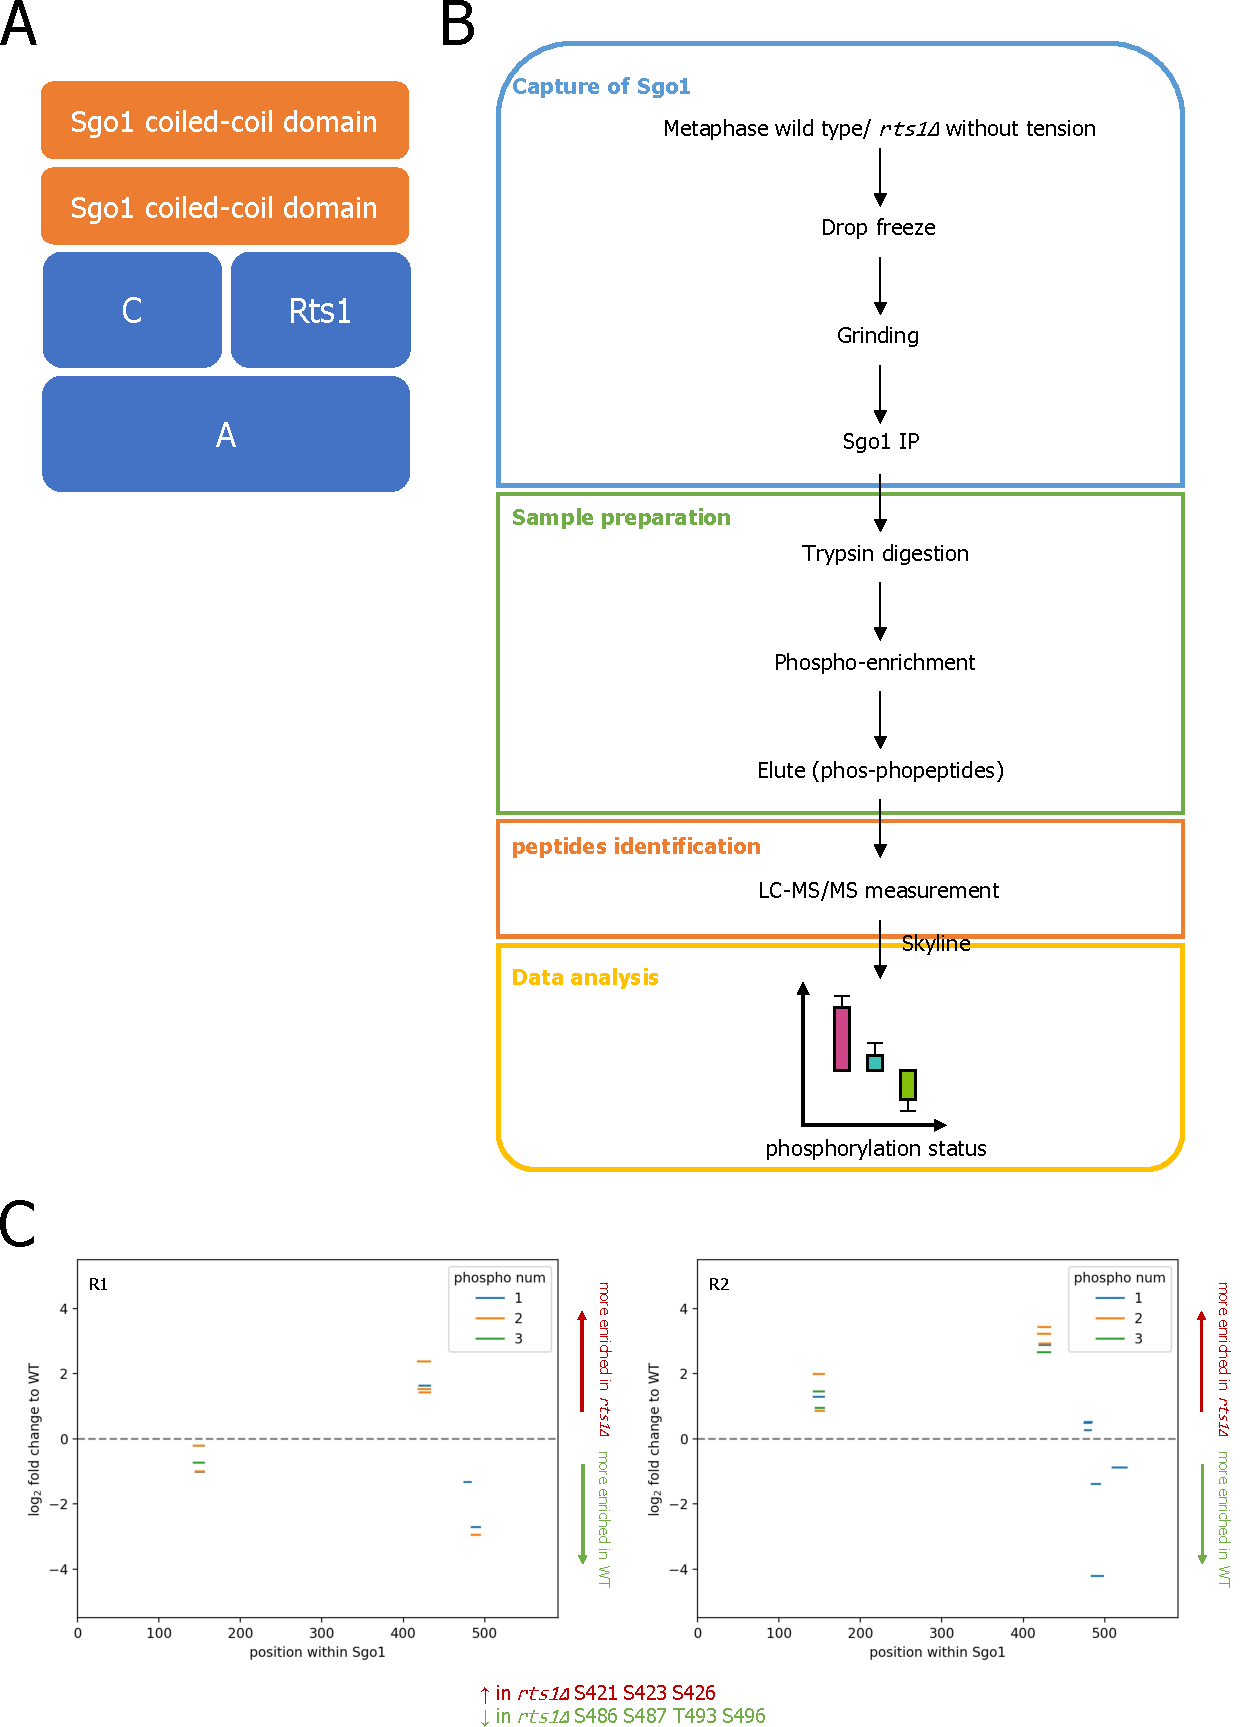
\includegraphics[width=0.9\textwidth]{chapter3/figures/Sgo1 phospho in rts1d.pdf}
  \caption[IP-MS detected changes in Sgo1 phosphorylation in the absence of Rts1]{IP-MS detected changes in Sgo1 phosphorylation in the absence of Rts1. (A) Cartoon of Sgo1-PP2A interaction (revised from \cite{Xu2009StructureInteraction}). (B) Schematics of the Sgo1 IP-MS experiment (C) relative intensities of phosphorylated Sgo1 peptides between wild type and \textit{rts1$\Delta$}. Each bar indicates a single Sgo1 peptide with amino acids of Sgo1 indicated on the x-axis. mono-, di- and tri-phosphorylated forms of the same peptide are indicated by differently coloured bars. Amino acid residues potentially more phosphorylated in \textit{rts1$\Delta$} are marked in red and those potentially less phosphorylated are marked in green. }
  \label{fig:sgo1phosphorts1d}
\end{figure}

\nomenclature{IP}{ImmunoPrecipitation}

\subsection{Sgo1 re-localization is independent of the phosphorylation at S421 or S487}

To test the functional relevance of the potential Sgo1 phosphorylation regulated by PP2A-Rts1, I wanted to measure the benomyl sensitivity of Sgo1 phospho-mutants to assess the functionality of their Sgo1 proteins. Therefore, I picked one site from each group identified as down-regulated or up-regulated by PP2A-Rts1 in the previous experiment and acquired both the phospho-null and phospho-mimic mutants from the Marston lab yeast collections. Wild type and \textit{sgo1$\Delta$} were included as the positive and negative control. The result of the spot assay was shown in Figure~\ref{fig:sgo1phosphomutants}A. \textit{sgo1$\Delta$} indicated strong sensitivity to benomyl as expected. Interestingly, the phospho-null mutant of the down-regulated site (S421A) and the phospho-mimic mutant of the up-regulated site (S487D) showed mildly increased viability compared to wild type on the benomyl-containing plate whereas their opposite phospho-mutants (S421D and S487A) had slightly reduced viability. This suggests that Sgo1 phosphorylation regulated by PP2A-Rts1 is relevant to its mitotic functions. However, \textit{rts1$\Delta$} also showed comparable benomyl sensitivity to the wild type, arguing against the idea. 

Since the aim of the project is to understand the mechanism of Sgo1 localisation regulation, I decided to leave the confusion aside and directly investigated the localisation of Sgo1 in those mutants. Hence, I used live-cell imaging to determine the duration of Sgo1 staying at the peri-centromere as in the previous experiments (Figure~\ref{fig:sgo1phosphomutants}B). As measured before, the duration of Sgo1-EGFP being as foci had a median of 30 \si{\minute}. The phospho-mutants were not statistically different from the wild type, suggesting that, whether genuinely phosphorylated or not, these sites are not involved in regulating Sgo1 localisation. Thus, I concluded that Sgo1 re-localization is independent of the phosphorylation at S421 or S487 (Figure~\ref{fig:sgo1phosphomutants}C). 

\begin{figure}[htbp]
  \centering
  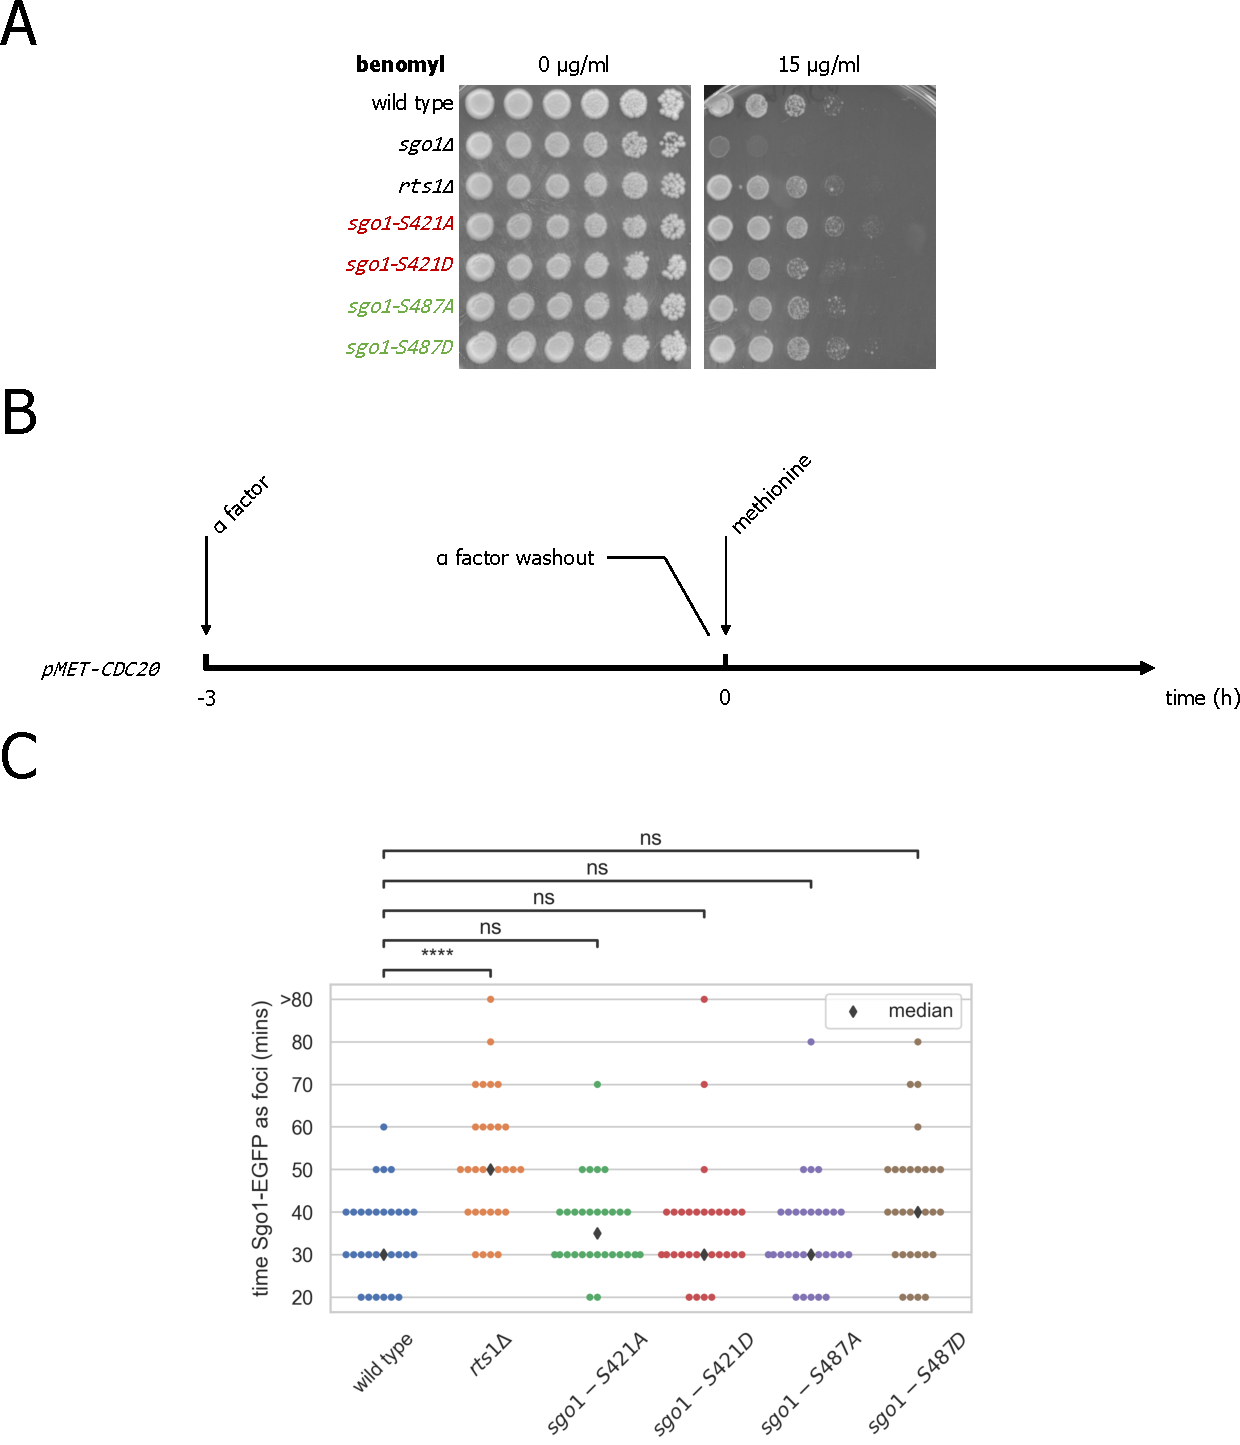
\includegraphics[width=0.9\textwidth]{chapter3/figures/sgo1 phospho mutants.pdf}
  \caption[Phenotypical characterisation of mutants with putative PP2A-Rts1-regulated phosphorylation sites of Sgo1 mutated]{Phenotypical characterisation of mutants with putative PP2A-Rts1-regulated phosphorylation sites of Sgo1 mutated. (A) Spot assay testing the benomyl sensitivity of the strains. Five-fold serial dilutions of indicated strains spotted on rich medium with 0 or 15 \si{\micro\gram/\milli\litre} benomyl. The red and green colours indicate whether the site is potentially more or less phosphorylated in \textit{rts1$\Delta$}. (B) Schematics of the imaging experiment. (C) Quantification of the time of Sgo1-EGFP signal being visualised as foci. The two-tailed independent t-test was used to calculate statistical significance. (****) P<0.0001; (ns) not significant. }
  \label{fig:sgo1phosphomutants}
\end{figure}

\subsection{PP2A-Rts1 is required for timely sister kinetochore separation}

On the contrary to the phospho-mutants, \textit{rts1$\Delta$} did show a 20-\si{\minute} increase in the time Sgo1-EGFP being visualised as foci in Figure~\ref{fig:sgo1phosphomutants}C, which is in consistency with \cite{Nerusheva2014}. This suggests PP2A-Rts1 is required for the timely removal of Sgo1 from the peri-centromere. However, the lack of information on inter-kinetochore distance in that experiment prevented us from distinguishing between (A) PP2A-Rts1 is the phosphatase de-localising Sgo1, likely by de-phosphorylating H2A-pS121, and (B) PP2A-Rts1 is required to generate enough tension for Sgo1 re-localisation on time. Therefore, I decided to include the inter-kinetochore distance measure in the experiment. Besides, The PP2A-binding-defective mutant \textit{sgo1-3A} was also included to study if the interaction is important here. The standard G1-to-metaphase live-cell imaging was conducted as previously described (Figure~\ref{fig:sgo1rts1mutants}A). Notably, by the time I performed the experiment, the camera of our wide-field microscope was swapped to Photometrics Prime 95B due to a product demonstration, resulting in a different-sized field of view from the previous experiments (Figure~\ref{fig:sgo1rts1mutants}B). In spite of that, the dynamics of Sgo1-EGFP localisation and inter-kinetochore distance of the wild type are the same as before. The result indicated that, despite a 15-\si{\minute} delay in the emergence, the vanish of Sgo1-EGFP foci was around 30 \si{\minute} later in \textit{rts1$\Delta$} (Figure~\ref{fig:sgo1rts1mutants}C). This leads to a 15-\si{\minute} increase in the duration of Sgo1 staying as foci, which is comparable to the results in Figure~\ref{fig:sgo1phosphomutants}C and \cite{Nerusheva2014}. However, when examining the inter-kinetochore distance, \textit{rts1$\Delta$} showed about 30 \si{\minute} delay than the wild type (Figure~\ref{fig:sgo1rts1mutants}C), indicating that PP2A-Rts1 is also required for timely separation of sister kinetochores. This means that the delay in Sgo1 de-localisation in \textit{rts1$\Delta$} is likely due to its delayed tension establishment, arguing against the hypothesis that PP2A-Rts1 is the phosphatase directly removes Sgo1. It can also be supported by the observation that the inter-kinetochore distance for Sgo1 to disperse was roughly the same between \textit{rts1$\Delta$} and the wild type. In further support, \textit{sgo1-3A}, whose Rts1 centromeric enrichment is abolished in mitosis \citep{Eshleman2014}, showed a very similar Sgo1-EGFP and Mtw1-tdTomato dynamics to the wild type (Figure~\ref{fig:sgo1rts1mutants}C). 

As mentioned before, Sgo1 association with the peri-centromere chromatin was increased in \textit{rts1$\Delta$} in the absence of tension. Apart from its original aim, this imaging experiment also provided an opportunity to alternatively test the finding. Hence, I quantified the fluorescence intensities of Sgo1-EGFP foci for the wild type and \textit{rts1$\Delta$} while tension was not established. Surprisingly, there was no significant difference observed (Figure~\ref{fig:sgo1rts1mutants}D). One possible explanation is that, albeit the total amount remains similar, the turnover rate of peri-centromeric Sgo1 might be reduced in \textit{rts1$\Delta$}, resulting in increased ChIP signal. 

\begin{figure}[htbp]
  \centering
  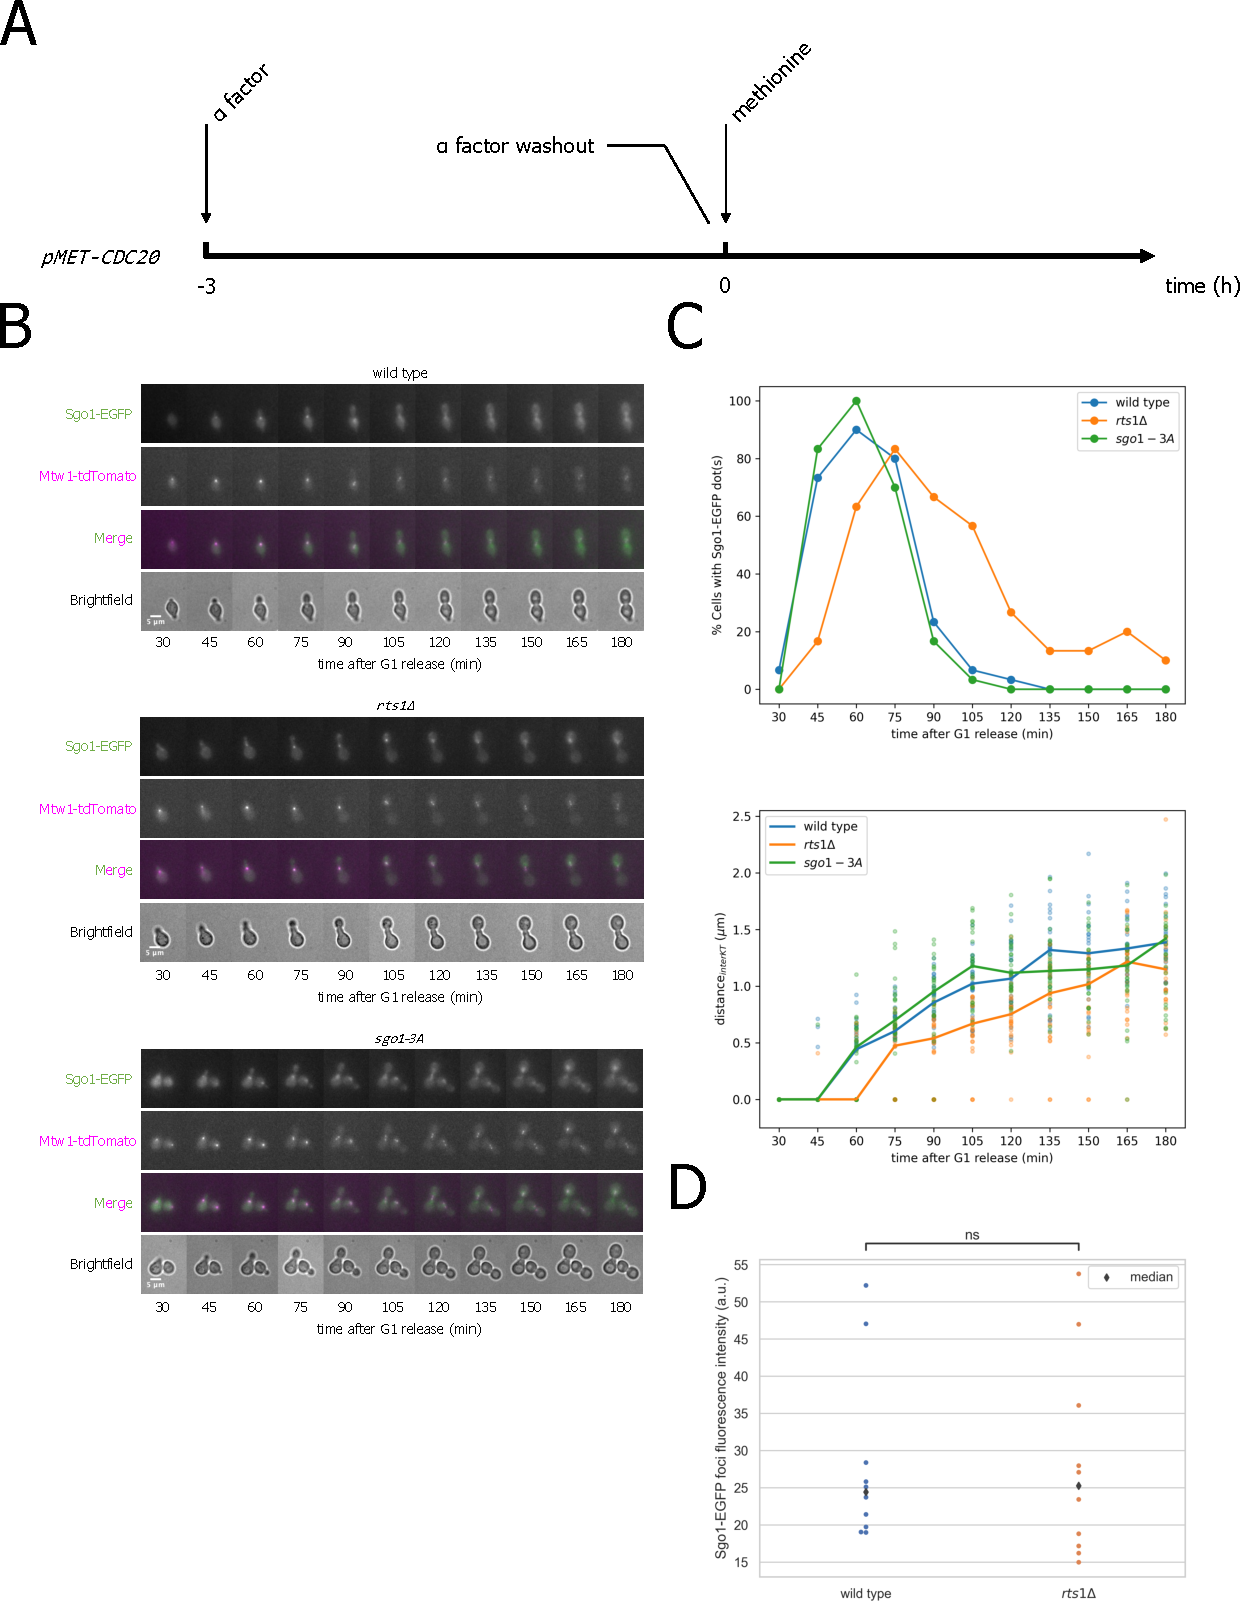
\includegraphics[width=0.9\textwidth]{chapter3/figures/Sgo1 rts1 mutants.pdf}
  \caption[PP2A-Rts1 is required for timely sister kinetochore separation but not for reducing Sgo1 level at peri-centromere]{PP2A-Rts1 is required for timely sister kinetochore separation but not for reducing Sgo1 level at peri-centromere. (A) Schematics of the imaging experiment. (B) Montages of representative time-lapse imaging. (C) N=30 cells for each strain were followed over time and quantified. Top panel: the percentage of cells with Sgo1-EGFP foci was shown as a function of time. Bottom panel: median inter-kinetochore distance as a function of time. Individual data points are shown as dots. (D) N=10 cells for the wild type and \textit{rts1$\Delta$} were quantified for the highest fluorescence intensities of Sgo1-EGFP foci among all frames. (ns) not significant.}
  \label{fig:sgo1rts1mutants}
\end{figure}

\subsection{Tension induces mild chromosome condensation}

Interphase chromosomes have to be condensed during mitosis to reduce space occupied, remove sister chromatids catenation, provide physical properties able to withstand forces during movement and therefore facilitate faithful chromosome segregation \citep{Antonin2016ChromosomeMitosis, Piskadlo2016NovelCondensation, Beseda2020MitoticVariability, Takahashi2019FoldingChromosomes}. The current model of chromosome condensation recognises it to be driven by the condensin-mediated compaction pathway and histone-mediated contraction pathway in parallel \citep{Wilkins2014, Kruitwagen2015}. Interestingly, key players from both pathways have been reported to interact with shugoshin or the H2A phosphorylation enabling Sgo1 chromatin association, including Topoisomerase II \citep{Zhang2020FunctioningMitosis} and condensin itself \citep{Verzijlbergen2014, Yahya2020} from the condensin-mediated pathway and CPC \citep{Abad2022MechanisticCPC} from the histone-mediated pathway. This makes Sgo1 and H2A phosphorylation potentially important in chromosome condensation. Indeed, in budding yeast, both compaction and contraction were impaired in the absence of Sgo1 \citep{Kruitwagen2018}. 

Our previous finding that H2A-pS121 and possibly Sgo1 re-distribute from the centromere to the whole genome by tension provides a potential molecular explanation for the model proposed by \cite{Kruitwagen2018}, where SAC silencing is required for further chromosome condensation. If it is true, we would expect increased chromosome condensation upon the establishment of tension. Hi-C has been used to investigate chromosome condensation in various species \citep{Kakui2017Condensin-mediatedYeast, Schalbetter2017SMCContext, Lazar-Stefanita2017CohesinsCellcycle, Naumova2013OrganizationChromosome}. To test the hypothesis, I took advantage of Hi-C experiments conducted by \cite{Paldi2020ConvergentPericentromeres} and compared data from metaphase cells with and without tension. The Hi-C ratio map revealed the conformational changes in peri-centromere chromatin by tension, indicated by the red cross around the core centromeres, as reported in the paper (Figure~\ref{fig:Hi-C+-tension}A). Besides, the tension sample showed increased inter-centromere contact (the blue dots at the intersection of centromeres of different chromosomes) and increased inter-arm contact (the blue 'wings' extending diagonally from the centromeres). Importantly, It indicated a mild increase in long-range \textit{in cis} contact (the two light blue lines beside the diagonal) and a mild decrease in short-range contact (the light red line along the diagonal), both of which are the characteristics of chromosome condensation described by \cite{Kakui2018SMCLandscape}. As an alternative to the ratio map, I also visualised the Hi-C difference map, where the contact probability at each coordinate of one sample is simply subtracted by that of the other one (Figure~\ref{fig:Hi-C+-tension}B). Consistently, it also revealed the mild increase in long-range \textit{in cis} contact and the decrease in short-range contact. The Hi-C difference further showed blue dots along the diagonal, which might represent increased loop formation in the tension sample. To obtain a more quantitative view, the contact probabilities of the genome excluding the centromeres were plotted as a function of distance (Figure~\ref{fig:Hi-C+-tension}C). Albeit to a mild extent, the difference between curves of tension and no tension sample did mimic the difference between interphase and mitosis in different species \citep{Kakui2018SMCLandscape}. The contact probabilities of the tension sample showed a reduction in the distances less than 20 kb, an increase in 20 to around 150 kb and another decrease in distances greater, which can also be inferred from the slope plot below. This is in good quantitative agreement with other chromosome condensation research using budding yeast, where the interval of increased contact probability was observed between 10 to 100 kb \citep{Kakui2018SMCLandscape, Schalbetter2017SMCContext, Lazar-Stefanita2017CohesinsCellcycle}. Notably, the increase in long-range interaction was stronger at chromosomal regions further away from the centromeres, a phenomenon that has been reported in budding yeast chromosome condensation \citep{Neurohr2011ALength}. Visualisation of individual chromosomes identified a strong increase in long-range interaction at chrXII, where rDNA was located, further supporting that the difference observed here is due to genuine chromosome condensation rather than artefacts from data analysis. Therefore, I concluded that a mild chromosome condensation is induced upon the establishment of tension. 

\begin{figure}[htbp]
  \centering
  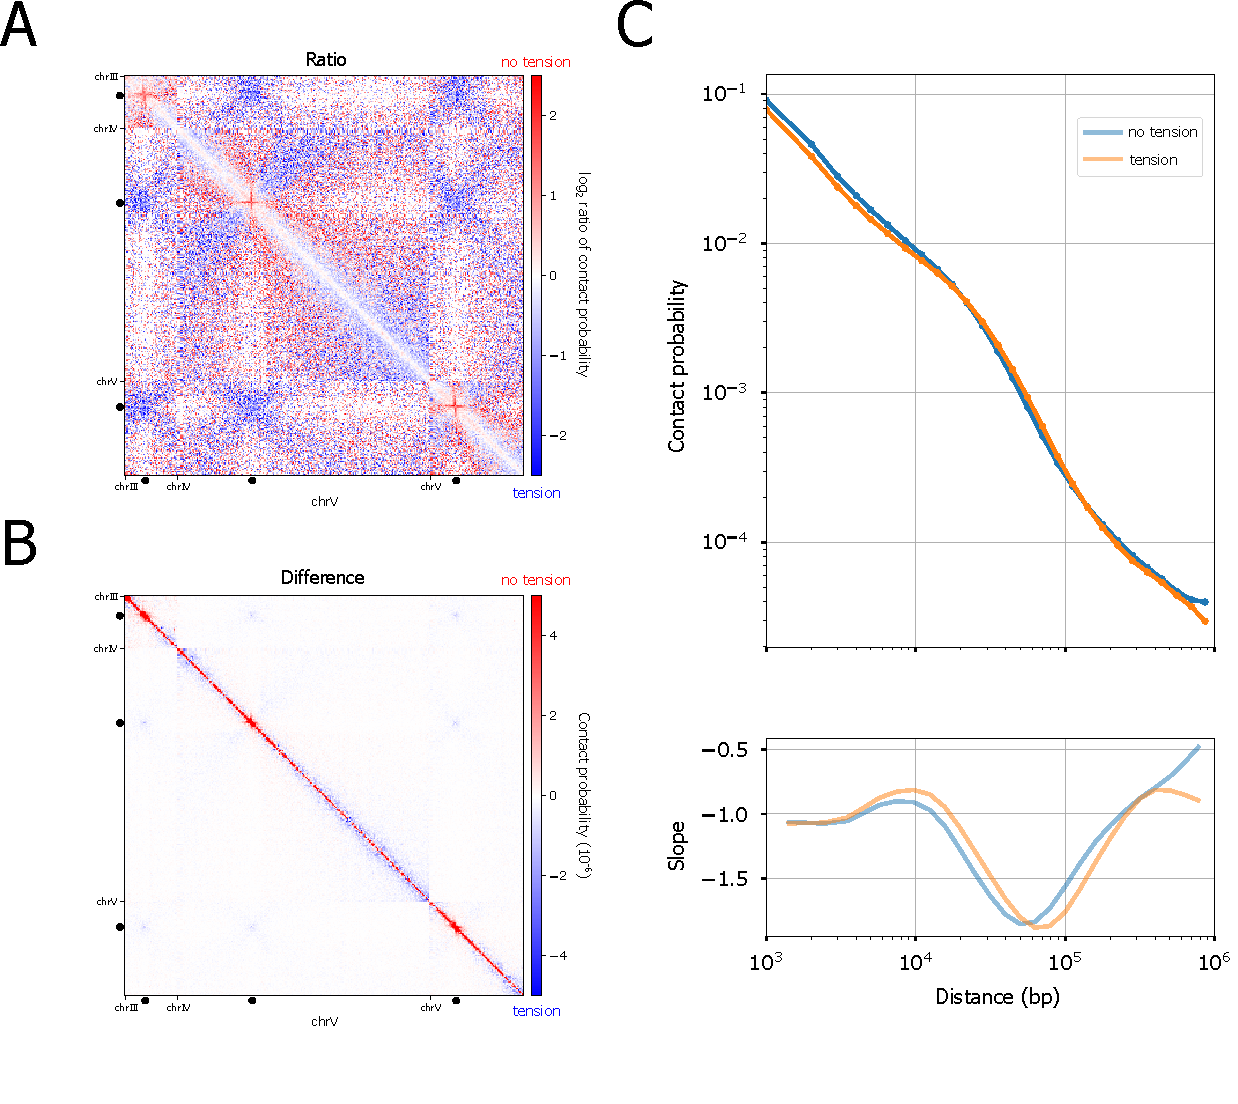
\includegraphics[width=0.9\textwidth]{chapter3/figures/+-tension Hi-C.pdf}
  \caption[Long-range \textit{in cis} interactions are mildly increased upon the establishment of tension]{Long-range \textit{in cis} interactions are mildly increased upon the establishment of tension. (A-C) Analyses of Hi-C of cells arrested in metaphase with or without tension from \cite{Paldi2020ConvergentPericentromeres}. (A) Hi-C ratio map (5kb binning) of chromosome III, IV and V. Black dots represent the coordinates of the core centromeres. (B) Hi-C difference map (5kb binning) of chromosome III, IV and V (no tension - tension). Black dots represent the coordinates of the core centromeres. (C) Top: median contact probability as a function of genomic distance, excluding contacts across the 50kb regions flanking the core centromeres. Bottom: The slopes of the curves above.}
  \label{fig:Hi-C+-tension}
\end{figure}

\subsection{Cohesin is not required for the concentration of Sgo1 at centromere-proximal location}

In the absence of tension, the association of Sgo1 with chromatin shows three major peaks, at the core centromere and the two peri-centromeric borders \citep{Verzijlbergen2014, Paldi2020ConvergentPericentromeres}. Intriguingly, this is different from H2A-pS121, whose distribution profile is rather bell-shaped (Figure~\ref{fig:sgo1comparison}). Given its necessary role in localising Sgo1, this result is quite surprising and it suggests that there might be other factors determining Sgo1 localisation. It has been shown in humans that interaction with cohesin is key to Sgo1 localisation to the inner centromere \citep{Liu2013a}. Also, in budding yeast, cohesin depletion results in a reduction in the ChIP signal at the centromeric region \citep{Verzijlbergen2014}. These results supported the idea that cohesin could be the factor mentioned above. However, this is in contradiction with the experiment used to demonstrate shugoshin's function in tension sensing, where Sgo1 is shown to be required for delaying cell cycle progression upon cohesin depletion \citep{Indjeian2005a}. As kinetochore-microtubule attachment is undisturbed, this experiment implies that Sgo1 should be localised at the peri-centromere to maintain CPC localisation for error correction. 

\begin{figure}[htbp]
  \centering
  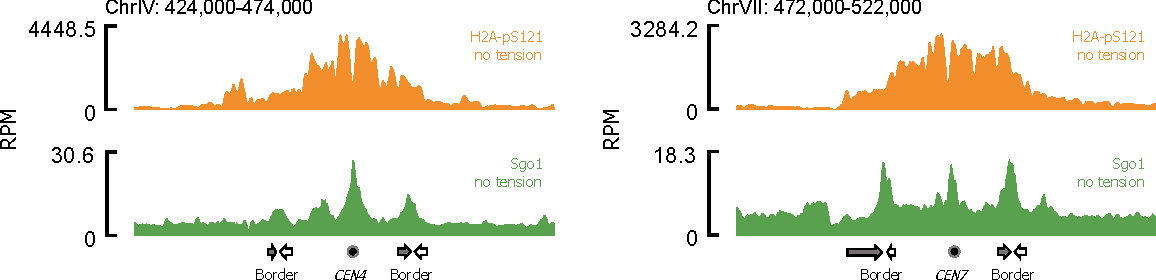
\includegraphics[width=0.9\textwidth]{chapter3/figures/Sgo1 comparison.pdf}
  \caption[H2A-pS121 ChIP-seq profile is qualitatively different from Sgo1]{H2A-pS121 ChIP-seq profile is qualitatively different from Sgo1. ChIP-seq profiles of H2A-pS121 and Sgo1 \citep{Paldi2020ConvergentPericentromeres} at the 50kb regions of chromosome IV and VII centromeres. Convergent genes at the peri-centromere borders are marked as arrows. }
  \label{fig:sgo1comparison}
\end{figure}

To solve the enigma, we sought to investigate the localisation of Sgo1 upon cohesin depletion by microscopy method. Cells used for Sgo1-EGFP imaging that additionally bear \textit{pMET-SCC1} were used and the experimental procedure was the same as the one in Figure~\ref{fig:bub1metscc1} (Figure~\ref{fig:sgo1metscc1}A). Surprisingly, unlike the wild type, Sgo1-EGFP remained its foci signal till the end of the experiment in \textit{pMET-SCC1} (Figure~\ref{fig:sgo1metscc1}B and C). This result is in favour of the classic genetics experiment \citep{Indjeian2005a} but is against the ChIP-qPCR results \citep{Verzijlbergen2014}. It might again reflect the fundamental difference in methodology principles between ChIP and fluorescence microscopy as in Figure~\ref{fig:sgo1rts1mutants}. Another possible explanation is that cohesin is not required for the recruitment of Sgo1 to the centromeric region but for its subtle localisation to a more confined sub-region as in humans \citep{Liu2013a}. Furthermore, the fact that Sgo1 localisation resembles Bub1 upon cohesin depletion (Figure~\ref{fig:bub1metscc1}) supports the notion from previous experiments that the localisation of Bub1 and H2A-pS121 is the determining factor of Sgo1 localisation. 

To ensure the efficacy of cohesin, I further conducted a mitotic time-course experiment using the \textit{pMET-SCC1} strain in the presence and absence of methionine, followed by western blotting to measure the expression level of Scc1. Spindle IF was used to determine the stages of the cell cycle (Figure~\ref{fig:sgo1metscc1}D). Albeit the sub-optimal synchronisation (Figure~\ref{fig:sgo1metscc1}E), it can still be seen that cells went through metaphase and anaphase in the absence of methionine, whereas they were arrested in metaphase when methionine was added. As expected, without methionine, Scc1 accumulated since the G1 release but started to decrease upon anaphase onset, accompanied by the emergence of the band at lower molecular weight, which represents the cleaved products \citep{Alexandru2001PhosphorylationYeast}. In the presence of methionine, the lack of the band representing cleaved products agreed with the metaphase arrest indicated by the spindle IF (Figure~\ref{fig:sgo1metscc1}E). Importantly, at the same exposure time, the Scc1 signal is largely reduced compared to no Scc1 depletion but still remained visible, suggesting an incomplete depletion (Figure~\ref{fig:sgo1metscc1}D). Therefore, we could not rule out the possibility that residual cohesin is sufficient to support the concentration of Sgo1-EGFP at centromere proximity. 

\begin{figure}[htbp]
  \centering
  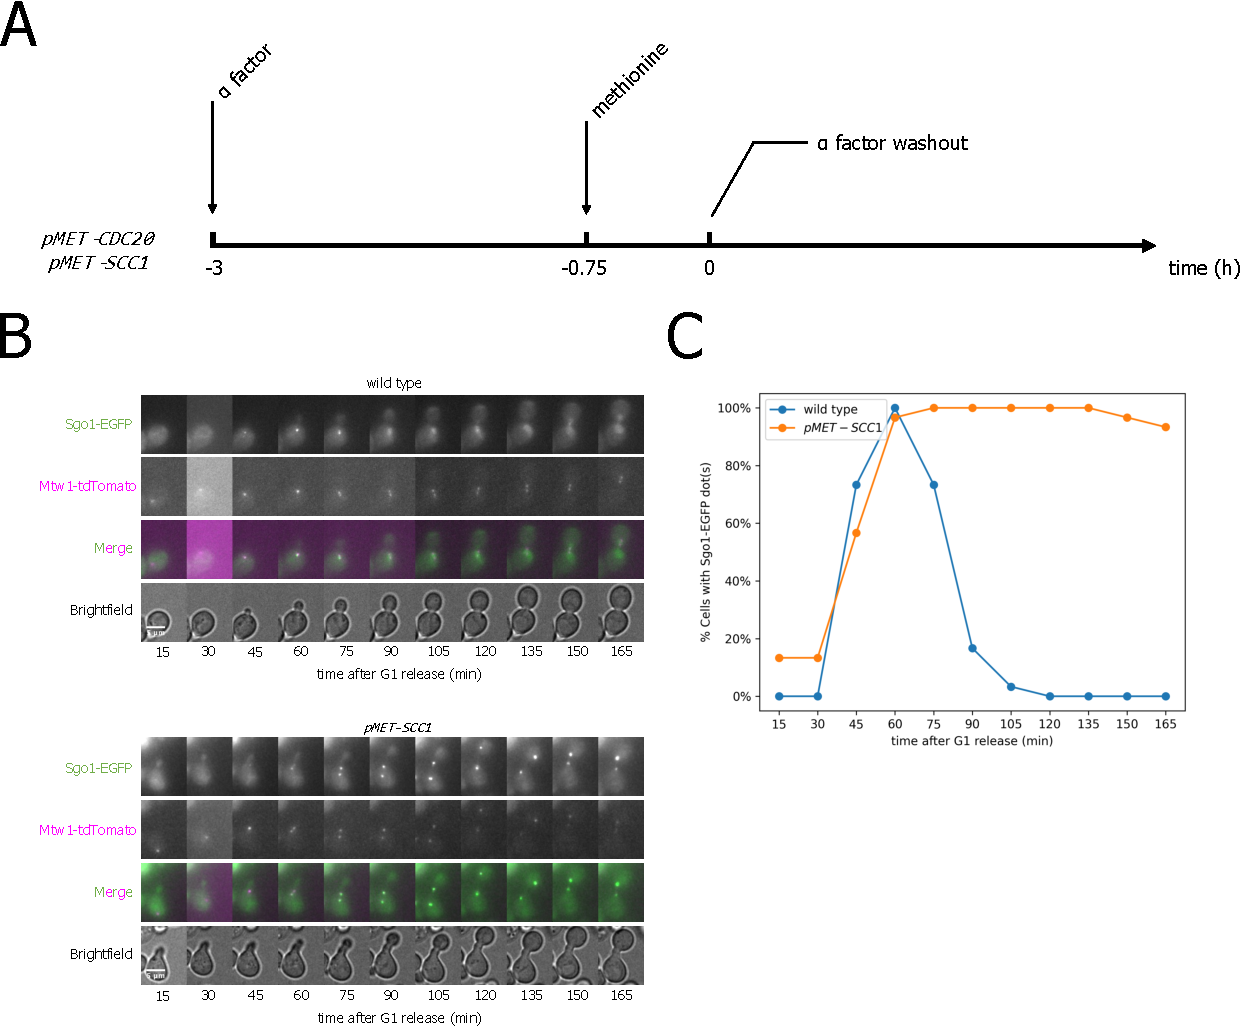
\includegraphics[width=0.9\textwidth]{chapter3/figures/Sgo1 pMET-SCC1.pdf}
  \caption[Sgo1 remains concentrated proximal to the centromere upon cohesin depletion]{Sgo1 remains concentrated proximal to the centromere upon cohesin depletion. (A) Schematics of experimental procedures. (B) Montages of representative time-lapse imaging. (C) N=30 cells for each strain were followed over time and quantified. The percentage of cells with Sgo1-EGFP foci was shown as a function of time. (D) Western blotting on cells arrested in metaphase without tension using anti-myc antibody to detect the expression level of Scc1-myc18. Pgk1 was used as the loading control. (E) The proportion of cells with metaphase or anaphase spindle over time by tubulin IF.}
  \label{fig:sgo1metscc1}
\end{figure}

\nomenclature{qPCR}{quantitative Polymerase Chain Reaction}
\nomenclature{RPM}{Reads Per Million}

\section{Discussion}
\subsection{Model for tension-dependent re-localisation of Sgo1}

Tension-dependent re-localisation of Sgo1 has been observed in various species and shown to be functionally important. To understand the mechanism by which budding yeast Sgo1 is re-localised under tension, we started with a naive model (Figure~\ref{fig:naive}) where the balance between Bub1 and a counteracting phosphatase determines the level of local phosphorylation important for the localisation of Sgo1, and tension is able to reduce the local activity of Bub1 at peri-centromere and hence flip the balance towards the phosphatase. Yet, questions remained to be answered for this model. It was unknown how Bub1 activity in a particular area is regulated by tension. Bub1 substrate H2A-S121 is known to be required for Sgo1 localisation but whether the regulation of its phosphorylation is the key to Sgo1 re-localisation was untested. Lastly, the identity of the phosphatase involved was also to be elucidated. 

The observations that Bub1 remains at the kinetochore after the establishment of tension \citep{Bokros2021YeastAnaphase, Nerusheva2014} and that contacts between the core centromere and the peri-centromere borders are reduced by tension \citep{Paldi2020ConvergentPericentromeres} led us to the hypothesis that tension could regulate local Bub1 activity by pulling kinetochore-localised Bub1 from its substrate(s) at the peri-centromere borders. However, the tetO arrays at one peri-centromere border stayed a similar distance to one of the Bub1-mNG foci regardless of the tension, making it difficult to draw a conclusion on this hypothesis (Figure~\ref{fig:periCEN}). Instead, it was noticed that the fluorescence intensity of Bub1 foci experienced a sharp decrease coinciding with the separation of sister kinetochores, suggesting the kinetochore localisation of Bub1 might be regulated by tension (Figure~\ref{fig:bub1mtw1}). This raised an alternative explanation that tension could de-localise Bub1 from the kinetochore and hence it is physically separated from its peri-centromeric substrate(s). A following experiment revealed that Bub1-mNG foci maintained their intensity when tension is abolished by cohesin depletion, indicating tension is indeed required for Bub1 de-localisation on top of kinetochore-microtubule attachment (Figure~\ref{fig:bub1metscc1}). The sufficiency of Bub1 removal for Sgo1 de-localisation was demonstrated by the prompt dispersal of Sgo1-EGFP foci upon Bub1 depletion (Figure~\ref{fig:bub1aid}). Moreover, with similar cell cycle progression, indicated by the inter-kinetochore distance, cells bearing \textit{Bub1-EGFP} had their fluorescence foci dimmed 15 \si{\minute} earlier than the ones bearing \textit{SGO1-EGFP}, suggesting Bub1 de-localisation happens before Sgo1 de-localisation (Figure~\ref{fig:bub1sgo1}). Though the experiment would be more solid if Bub1 and Sgo1 were tagged with fluorescence proteins of different colours, similar maturation time and sufficient brightness, in a single strain. Nevertheless, the experiments above pointed to the conclusion that the de-localisation of Bub1 from the kinetochore by tension is upstream Sgo1 tension-dependent re-localisation. 

Due to its well-established role in shugoshin localisation in various species and the fact that it is a substrate of Bub1, it is tempting to hypothesise that the phospho-regulation of H2A-S121 is the key to tension-dependent re-localisation of Sgo1. To test this idea, we made phospho-specific antibodies. It was found that this phosphorylation was quickly reduced when Bub1 is depleted, which fits the predicted behaviour of the substrate by the naive model (Figure~\ref{fig:ph2abub1aid}). In further support of the hypothesis, albeit the total H2A-pS121 remained at similar levels in the presence or absence of tension, ChIP-seq revealed distinct distributions over the genome, with the phosphorylation being more spread along the chromosome arms upon tension whereas more enriched at centromeres in the tension-less condition (Figure~\ref{fig:ph2achipseq2nd}). This re-distribution corresponds well with the re-localisation of Sgo1, making H2A-S121 plausible to be the substrate in the naive model. However, the notion is in contradiction with the results by \cite{Nerusheva2014} that Sgo1 can still be localised to the peri-centromere in the H2A phospho-mimic mutant H2A-S121D in a Bub1-dependent manner. It was then noticed a likely strain confusion in those experiments (Figure~\ref{fig:h2as121dseq}). ChIP-qPCR experiment with re-constructed strains showed a low association of Sgo1 with peri-centromeric chromatin in the phospho-mimic mutant, indicating that Sgo1 cannot be concentrated if the H2A phosphorylation is homogeneously distributed over the genome, which emphasised the importance of the spatial regulation of H2A-pS121 to Sgo1 localisation (Figure~\ref{fig:sgo1chiph2amutants}). The conclusion is further confirmed by the results from an imaging experiment, where Sgo1-EGFP did not form any focus in the H2A phospho-mimic mutant (Figure~\ref{fig:sgo1imagingh2amutants}). Therefore, I concluded that the re-distribution of H2A-pS121 is likely to underlie the re-localisation of Sgo1. 

Regarding the phosphatase counteracting Bub1 to de-phosphorylate H2A-pS121, we hypothesised PP1 and PP2A-Rts1 as potential candidates. Interestingly, \textit{GLC7}, the gene encoding the PP1 catalytic subunit, showed genetic interaction with \textit{SGO1}, indicated by that \textit{sgo1$\Delta$} is able to suppress the temperature sensitivity of \textit{glc7-10} and \textit{glc7-12} mutant (Figure~\ref{fig:growthassay}). Microscopy then revealed that Sgo1-EGFP foci did not vanish even though enough tension had been generated in those mutants, showing that PP1 is required for the re-localisation of Sgo1 (Figure~\ref{fig:sgo1glc712} and Figure~\ref{fig:sgo1glc710}). Nevertheless, Bub1 depletion after Sgo1 had been localised still caused quick dispersal of Sgo1-EGFP foci despite PP1 being inactivated, suggesting that the requirement of PP1 for Sgo1 de-localisation is unlikely due to direct counteracting of Bub1 activity (Figure~\ref{fig:bub1aidglc712}). Due to the complexity of this experiment, an easier method would be simply monitoring H2A-pS121 in the same condition by western blotting. It was later found that the kinetochore fluorescence intensity of Bub1-mNG was maintained upon PP1 inactivation, showing PP1 being also required for Bub1 de-localisation (Figure~\ref{fig:bub1glc712}). Hence, it is likely that PP1 is required for Sgo1 re-localization due to its role in de-localising Bub1. Rts1 has been shown to decrease Sgo1 association with peri-centromeric chromatin in the absence of tension \citep{Nerusheva2014}. However, the fluorescence intensity of Sgo1-EGFP foci in \textit{rts1$\Delta$} was not significantly different from that of the wild type, arguing an opposite interpretation. Furthermore, Sgo1-EGFP was de-localised at a similar inter-kinetochore distance with the wild type in \textit{rts1$\Delta$}, indicating PP2A-Rts1 is not required for the sensitivity of Sgo1 localisation to tension (Figure~\ref{fig:sgo1rts1mutants}). Thus, whether PP2A-Rts1 is the phosphatase de-phosphorylating H2A-pS121 was not further investigated. In conclusion, neither PP1 nor PP2A-Rts1 appears to be the phosphatase predicted by the naive model, though it could be complicated by possible redundancy, where more than one phosphatase can de-phosphorylate H2A-pS121. 

Based on the results from the experiments above, we proposed the following model for the tension-dependent re-localisation of Sgo1 in budding yeast. H2A-pS121 is responsible for Sgo1 recruitment and its level is determined by the kinase-phosphatase balance between Bub1 and an unknown phosphatase (Figure~\ref{fig:finalmodel}A). In the tension-less situation, SAC remains ON and Bub1 is localised at the kinetochore, causing a restricted, high kinase activity at spatially proximal chromatin. H2A-S121 at the peri-centromere is thus highly phosphorylated and concentrates Sgo1 locally. Upon the establishment of tension, SAC is turned OFF and Bub1 is de-localised from the kinetochore. Meanwhile, diffusing Bub1 reaches chromosome arms. Together, the shift of local kinase-phosphatase balance at both regions leads to a re-distribution of H2A-pS121 from the peri-centromere to chromosome arms. Sgo1 is then re-localised following this re-distribution (Figure~\ref{fig:finalmodel}B). 

\begin{figure}[htbp]
  \centering
  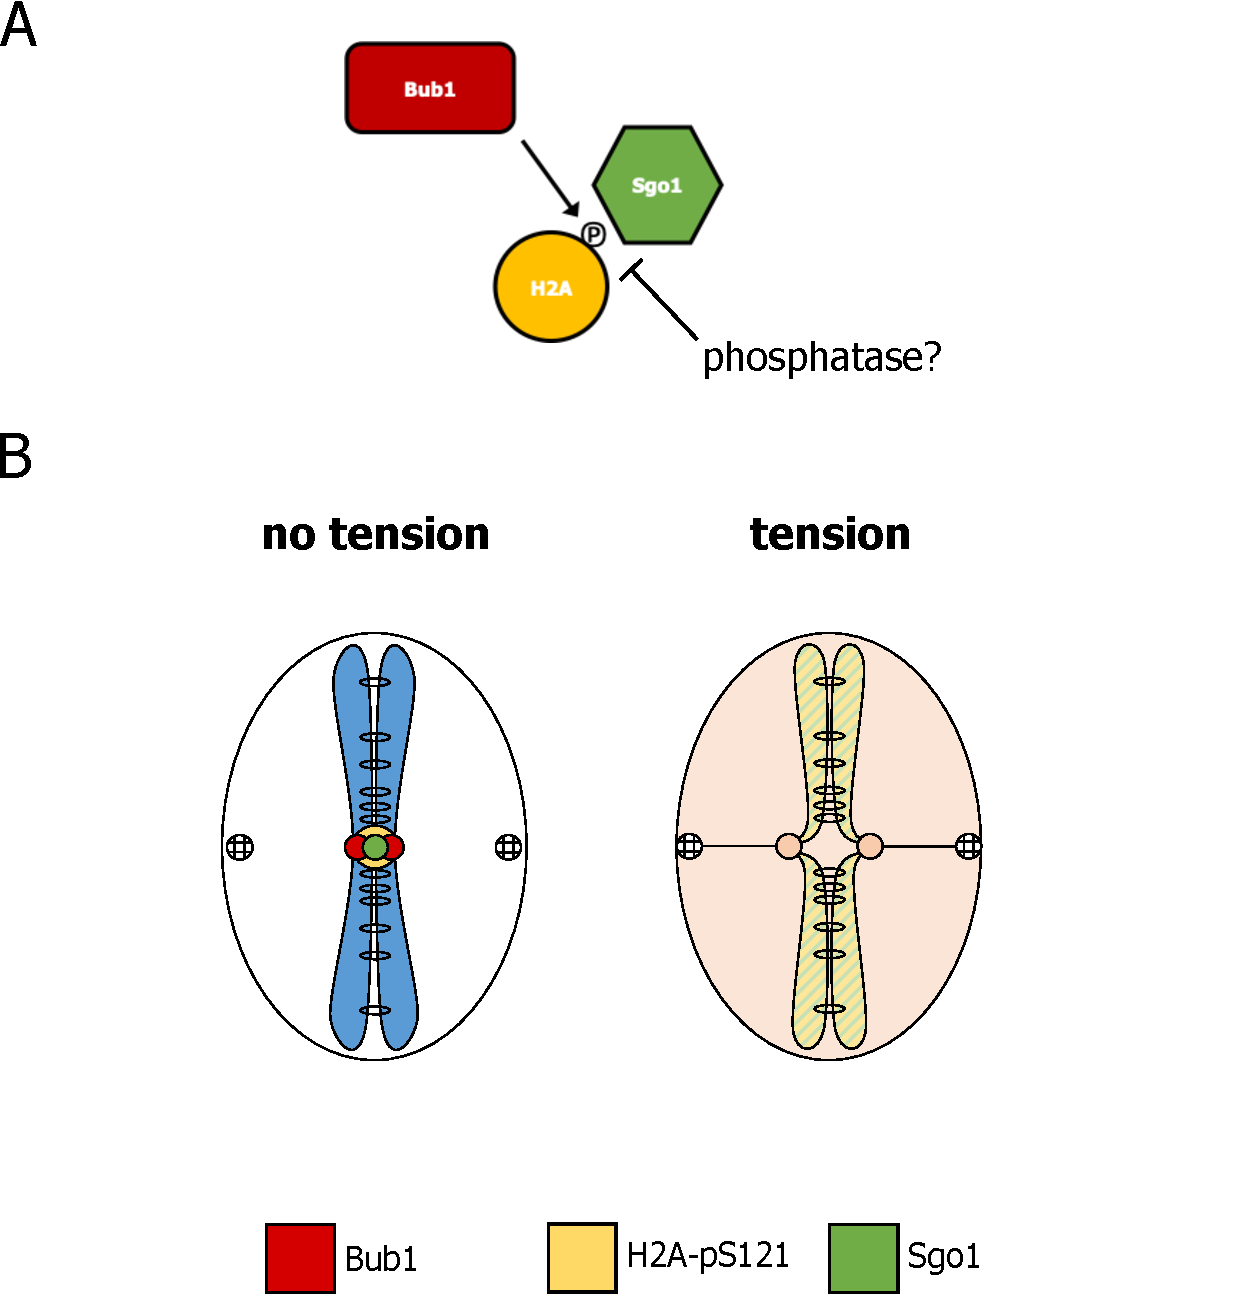
\includegraphics[width=0.9\textwidth]{chapter3/figures/graphic_model_final.pdf}
  \caption[Schematics of tension-dependent re-localisation of Sgo1]{Schematics of tension-dependent re-localisation of Sgo1. (A) Molecular machinery determining the localisation of Sgo1. The balance between Bub1 kinase and an unknown phosphatase determines the phosphorylation level of H2A at serine 121 and thus Sgo1 recruitment. (B) Spatial regulation of Bub1, H2A-pS121 and Sgo1 by tension. In the absence of tension, Bub1 is localised at the kinetochores and locally phosphorylates H2A at the peri-centromeric region, which then recruits Sgo1 to the peri-centromere. Upon the establishment of tension, Bub1 diffuses away from the kinetochore and reaches chromatin outside the peri-centromere, shifting the local kinase-phosphatase balance at both places. This leads to the H2A-S121 de-phosphorylation at the peri-centromere but phosphorylation at other parts of the genome, which titrates Sgo1 away from the peri-centromere.}
  \label{fig:finalmodel}
\end{figure}

This model (Figure~\ref{fig:finalmodel}B) processes the same notion as the yeast model proposed by \cite{Nerusheva2014} that opposing kinase and phosphatase are at the core of Sgo1 tension-dependent re-localisation. However, the details of the two models are rather different. \cite{Nerusheva2014} model proposes that tension increases the distance between kinetochore-localised Bub1 and its non-H2A-S121 substrate at the peri-centromere, leading to the de-phosphorylation by Sgo1-bound PP2A-Rts1 and eventually Sgo1 de-localisation. The differences between the two models majorly arise for three reasons. First, the analyses of G1-to-metaphase Bub1 live-cell imaging are different. \cite{Nerusheva2014} classified cells with the criteria that whether the Bub1 foci were visible by eye. Due to the persistence of Bub1 foci, the result was interpreted as Bub1 being removed from the kinetochore much later than Sgo1 re-localisation, leading to the hypothesis that kinetochore-bound Bub1 is pulled away from its substrate by tension. Whereas in this study, the fluorescence intensity of Bub1 foci was further quantified, which showed a sharp decrease around the same time, if not slightly earlier, when Sgo1 is re-localised. This observation brought up the possibility that Bub1 kinetochore localisation itself could be regulated by tension and it triggers downstream de-phosphorylation, which is revealed in the model proposed in this study. Second, the two models disagree on whether H2A-S121, the known Bub1 substrate important for Sgo1 localisation, is the key substrate regulated in the process. As mentioned above, a likely strain confusion gave rise to the interpretation that Bub1 substrate other than H2A-S121 is the key to Sgo1 re-localisation in \cite{Nerusheva2014}. However, with re-constructed strains, experiments conducted in this study suggested the opposite. Third, \cite{Nerusheva2014} model recognises PP2A-Rts1 as the phosphatase de-phosphorylating Bub1 substrate because the Sgo1 ChIP signal at peri-centromere was increased in the absence of tension and that the duration of Sgo1 foci was increased by 15 \si{\minute} in \textit{rts1$\Delta$}. Nevertheless, repeating the imaging experiment in this study did not show higher fluorescence intensities of Sgo1 foci in \textit{rts1$\Delta$}, asking for an alternative interpretation of the ChIP data. Detailed analysis of inter-kinetochore distance indicated a similar value at which Sgo1 foci are dispersed between \textit{rts1$\Delta$} and the wild type, suggesting the delay observed in \cite{Nerusheva2014} was probably due to reduced tension. 

The human model for tension-dependent re-localisation of Sgo1 describes a very different picture \citep{Liu2013a}. In the model, upon the establishment of tension, Sgo1 is de-phosphorylated at T346 by an unknown phosphatase, which switches it from cohesin-bound to H2A-pT120-bound. Given that cohesin is enriched at the inner centromere while H2A-pT120 is proximal to the kinetochore, Sgo1 moves from the inner centromere towards the kinetochore-proximal chromatin. However, there is evidence suggesting that the yeast model proposed in this study (Figure~\ref{fig:finalmodel}B) could also be conserved in humans. The key event of our yeast model is the re-distribution of H2A-pS121, the yeast equivalent of human H2A-pT120. Interestingly, in humans, disruption of the kinetochore localisation of Bub1, either by a point mutation \citep{Asghar2015} or by fusing the Bub1 kinase domain to BubR1, which allows the kinase domain to be part of the diffusible MCC complex \citep{Wang2022SpatialMitosis}, could lead to a similar spread of H2A-pT120 to the chromosome arms. Notably, in both cases, the centromeric localisation of shugoshin proteins was comprised. Although \cite{Liu2013a} showed that H2A-pT120 remains at kinetochore-proximal chromatin under tension, \cite{Asai2020} reported a decrease in the IF intensities of H2A-pT120. It is possible that the difference here resembles what has been discussed above about the different interpretations of Bub1 live-cell imaging. Moreover, centromeric Bub1 and Sgo2 were reported to decrease upon tension in that research \citep{Asai2020}. Therefore, the sequential de-localisation of Bub1, H2A-pT120 and shugoshins might also exist in humans. A unified model can be proposed in combination with \cite{Liu2013a} model. Potentially, in human cells, tension both de-localises Bub1 from the kinetochore and de-phosphorylates Sgo1, resulting in the majority of Sgo1 being moved to chromosome arms while a small but observable portion remaining at the centromeric region. This might also be true in budding yeast, as residual Bub1 \citep{Nerusheva2014, Bokros2021YeastAnaphase}, H2A-pS121 (this study) and Sgo1 \citep{Paldi2020ConvergentPericentromeres} have been observed at the old locations after their re-distributions upon tension. 

The major limitation of the proposed model (Figure~\ref{fig:finalmodel}B) lies in the unidentified phosphatase. Using general phosphatase inhibitors might be a good start to test the idea. Nevertheless, various difficulties and artefacts from cell death, yeast cell wall and changed pH of media were encountered in those experiments, which will not be elaborated on here. Apart from it, a final proof of this model would be showing that Sgo1 is indeed localised at chromosome arms once tension is established. In favour of this idea, over-expressed Sgo1 can be detected on chromosome arms by ChIP in cycling budding yeast and the enrichment is largely dependent on Bub1 \citep{Clift2009}. However, available Sgo1 ChIP-seq in the presence or absence of tension did not show an obvious difference in arm enrichment \citep{Paldi2020ConvergentPericentromeres}. Yet, it is worth noting that this ChIP-seq was not calibrated and that the Sgo1 ChIP signal is barely distinguishable from noise due to its low protein abundance and the fact that it does not directly bind DNA. Because of the undissolved nuclear envelope of budding yeast in mitosis, it is unable to distinguish chromosome arm localisation from nuclear localisation by microscopy, leaving a direct test of the hypothesis challenging. 

Shugoshin has been proposed as the tension sensor which translates the mechanical force into biochemical signals that can be read by the cell \citep{Indjeian2005a, Nerusheva2014, Marston2015}. However, the sole dependence of Sgo1 localisation on Bub1 localisation found in this study makes it rather a signal transducer. Indeed, shugoshin processes feature beneficial for this role. Positive feedback of its own localisation has been reported in human cells \citep{Liang2019ACells} and budding yeast \citep{Roy2019}, which gives Sgo1 the potential to respond quickly to a signal. How is tension sensed by the cells then? Extensive research has been conducted and various, not necessarily mutually exclusive models have been proposed on this topic \citep{Hindriksen2017TheLocalization, McVey2021AuroraSegregation, Broad2020AuroraCells}. Data obtained in this study are in line with the model proposed by \cite{Roy2019} that PP1 is recruited to Spc105 (Knl1) upon tension to de-phosphorylate the MELT motifs and thus release Bub1. In support of this idea, human Knl1 has been reported to undergo conformational changes when tension is established \citep{Roscioli2020}. 

Further work is required to validate the yeast model proposed here. To draw a final conclusion about whether PP1 has a role in de-phosphorylating H2A-pS121, a time course experiment followed by H2A-pS121 western blotting, similar to Figure~\ref{fig:ph2abub1aid}, in PP1 temperature-sensitive mutants could be performed. Although suffered from the sub-optimal signal-to-noise ratio, it might still be worth conducting a calibrated Sgo1 ChIP-seq to distinguish whether Sgo1 is localised to chromatin arms or is dispersed to the nucleus after re-localisation. More advanced ChIP-seq-like technologies, such as CUT\&RUN sequencing, could also be considered. As for the human model of Sgo1 tension-dependent re-localisation, it is important to quantify the amount of Bub1, H2A-pT120 and shugoshins at centromeric regions, possibly by IF, before and after tension. Given the release of T2T \citep{Nurk2022TheGenome}, the first complete human reference genome that can cover the centromeres, sequencing-based technologies could also be applied to investigate the question now. 

\nomenclature{T2T}{Telomere-to-Telomere}
\nomenclature{MCC}{Mitotic Checkpoint Complex}

\subsection{The regulation of Bub1 localisation potentially links chromosome condensation to SAC status}

Chromosome condensation is essential to both mitosis and meiosis and has been observed since the $19
^{th}$ century, but the detailed molecular mechanisms remain unclear \citep{Antonin2016ChromosomeMitosis, Piskadlo2016NovelCondensation, Beseda2020MitoticVariability, Takahashi2019FoldingChromosomes}. 

The regulation of Bub1 localisation potentially links chromosome condensation to SAC status
A
Why was Bub1 and Sgo1 indicated in chromosome condensation
W
preliminary data only
to be verified
I
model agrees well with literature
chromosome condensation metaphase or anaphase?
all three shit are linked to the re-localisation of Bub1 from the kinetochore, SAC silencing hallmark
why after SAC
autonomous or not
F
sgo1d Hi-C
H2A A mutant Hi-C
condensin ChIP-seq
Top2 ChIP-seq
CPC/H3-S10 ChIP-seq
Hi-C all mutants
all +/- tension
A mutants better have both subtypes  mutated  

\subsection{Role of cohesin in localising Sgo1}

Role of cohesin in Sgo1 localisation
A
not required for coarse localisation
W
fine localisation remain to be dissected
I
Hongtao Yu might still be right
F
Sgo1 ChIP-seq in met-SCC1 (Could be tricky)
structural data and make mutants specifically abolish Sgo1 cohesin interaction and then ChIP-seq

\subsection{PP2A could regulate Sgo1 functions}

\section{Materials and methods}
\subsection{Budding yeast methods}
\subsubsection{Strain construction}
\subsubsection{Yeast spot assay}
\subsection{Microscopy methods}
\subsubsection{FRET}
The FRET experiment was performed on a Nikon Ti2 inverted microscope equipped with a 100x Plan ApoChromat NA 1.45 oil lens and Prime 95B CMOS (sCMOS) camera. Fluorophores were excited with GFP and emission in the mCherry channel was recorded. Subsequently, standard GFP-GFP and mCherry-mCherry excitation and emission were performed. 

bleed-through from both fluorophores to the FRET channel are subtracted in ImageJ using the following formula: 
Acceptor in FRET channel (Co-efficient A) =	Mean intensity of Acceptor using FRET set/ Mean intensity of Acceptor using acceptor set

Donor in FRET channel (Co-efficient B) = Mean intensity of Donor only using FRET filter set/ Mean intensity of Donor only using Donor filter set

FRET Specimen - (A * FRET Specimen using Acceptor filter set) - (B * FRET Specimen using Donor filter set)

Protocol

Use 3 samples

Acceptor Only
Donor Only
FRET Sample
Collect 5 images

Acceptor Only using Acceptor filter set
Acceptor Only using the FRET filter set
Donor Only using the Donor filter set
Donor Only using the FRET filter set
FRET Specimen Only using FRET filter set

reference \citep{Gordon1998QuantitativeMicroscopy}

\subsubsection{Live-cell imaging}
Cells bearing \textit{pMET-CDC20} from patches on -MET plates were inoculated in 10 \si{\milli\litre} of CSM -MET and incubated at RT with shaking at 250 rpm overnight. Cells were diluted to $OD_{600}$=0.2 in 10 \si{\milli\litre} of CSM -MET in the morning, incubating at RT with shaking at 250rpm for over 1 \si{\hour}, allowing cells to enter the exponential phase. Then, cells were re-diluted to $OD_{600}$=0.2 in 10 \si{\milli\litre} of CSM -MET and 10 \si{\micro\litre} of 10 \si{\micro\gram/\milli\litre} alpha factor was added for G1 synchronization. After 1.5 \si{\hour}, another 5 \si{\micro\litre} of 10 \si{\micro\gram/\milli\litre} alpha factor was added. 1.5 \si{\hour} later, shmoo morphology was checked by a light microscope to ensure G1 arrest. 1 \si{\milli\litre} of cell culture was transferred to a 1.5 \si{\milli\litre} Eppendorf tube and concentrated by centrifuging at 3000 rpm for 3 \si{\minute} then removing 700 \si{\micro\litre} of supernatant. 250 \si{\micro\litre} of concentrated cell culture was loaded onto an 8-well Ibidi dish pre-treated with concanavalin A (preparation see separate protocol) and incubated at RT on bench for 15 \si{\minute} to allow cells to bind the bottom of the dish. The supernatant was removed using a bench aspirator and cells were washed twice with 250 \si{\micro\litre} of SC. After the final wash, 250 \si{\micro\litre} of SC was added to each well for imaging. 

\nomenclature{MET}{METhionine}

\subsubsection{Using AID system in microscopy}

\subsubsection{Quantification of fluorescence intensity}

\nomenclature{RT}{Room Temperature}
\nomenclature{rpm}{revolutions per minute}

\subsection{Protein methods}
\subsubsection{Western blotting}
normal protein
H2A-pS121
\subsubsection{Western blotting with big gel}
\subsubsection{Generation of phospho-specific antibody for H2A-pS121}
\subsubsection{ChIP}
for qPCR
for seq
\subsubsection{IP-MS}
cell growth
drop freeze
grinding
ab to dynabeads
IP
Bradford
silver stain
dry SDS-PAGE
instant blue
in-gel digestion
stage-tip
phospho-enrichment
mass spec
\nomenclature{MS}{Mass Spectrometry}
\subsection{DNA methods}
\subsubsection{qPCR}

\begin{table}[htbp]
\centering
\renewcommand{\arraystretch}{1.5}
\caption{qPCR primers}
\label{tab:qpcr}
\resizebox{\textwidth}{!}{%
\begin{tabular}{ccccl}
\hline
\multicolumn{1}{c}{Species}            & \multicolumn{1}{c}{Locus}  & \multicolumn{1}{c}{Direction} & \multicolumn{1}{c}{Number} & \multicolumn{1}{c}{Sequence}                 \\
\hline
\multirow{2}{*}{\textit{S.cerevisiae}} & \multirow{2}{*}{CEN4(a)}   & Forward   & 794    & CCGAGGCTTTCATAGCTTA      \\
                                       &                            & Reverse   & 795    & ACCGGAAGGAAGAATAAGAA     \\
\multirow{2}{*}{\textit{S.cerevisiae}} & \multirow{2}{*}{CEN4(b)}   & Forward   & 8172   & GCCGAGGCTTTCATAGCTTA     \\
                                       &                            & Reverse   & 8173   & GACGATAAAACCGGAAGGAAG    \\
\multirow{2}{*}{\textit{S.cerevisiae}} & \multirow{2}{*}{ARM4}      & Forward   & 8175   & GCTACCACCAATAACACAGTTGAG \\
                                       &                            & Reverse   & 8176   & GTACCTTCCCTGATAATCCGTCT  \\
\multirow{2}{*}{\textit{S.cerevisiae}} & \multirow{2}{*}{peri-CEN4} & Forward   & 8599   & TGTAACGGTCATGGTTGTCTTC   \\
                                       &                            & Reverse   & 8600   & ACCTCATTCGTCATGTGAGAGA   \\
\multirow{2}{*}{\textit{S.pombe}}      & \multirow{2}{*}{CEN}      & Forward   & 2179   & CAGACAATCGCATGGTACTATC   \\
                                       &                            & Reverse   & 2180   & AGGTGAAGCGTAAGTGAGTG     \\
\multirow{2}{*}{\textit{S.pombe}}      & \multirow{2}{*}{OTR}  & Forward   & 2183   & GCGTCGGAAGGTTGAGAATA     \\
                                       &                            & Reverse   & 2184   & CTGCACTAGCAATTGGATCG  
\\
\hline                                                             

\end{tabular}%
}
\end{table}
\nomenclature{OTR}{OuTer Repeat}

\subsubsection{Library preparation for Illumina sequencing}
\subsection{Computational methods}
\subsubsection{Image analysis}
ImageJ
\subsubsection{ChIP-seq data analysis}
sparK
\subsubsection{MS data analysis}
Maxquant
\subsubsection{phospho-peptide analysis}
Skyline
\subsubsection{Hi-C data analysis}
HicExplorer 
cooltools
\subsubsection{Code availability}
\chapter{Discussion}

\section{Final discussion}

Accurate chromosome segregation is a fundamental requirement for eukaryotic life, which relies on the specialised locus called the centromere. The spatial regulation of critical proteins is the key to the realisation of centromeric function. This work aimed to study the spatial organisation and dynamics of two vital centromeric proteins, CENP-A and Shugoshins, and explore whether they are interrelated. In this chapter, the latter aim will be discussed based on the literature and data collected in this work. Furthermore, both experimental and theoretical approaches were adopted for this work, providing an opportunity to reflect on the use of the two methodologies in centromere biology research. 

\subsection{The potential link between the spatial pattern of CENP-A nucleosomes and tension sensing}

CENP-A nucleosomes display a non-random distribution at the centromere, where they form distinct islands interspersed by canonical H3 nucleosomes \citep{Blower2002ConservedHumans, Dunleavy2011H3.3Phase., Kyriacou2018}. On the other hand, the inner/ peri-centromeric localisation of Shugoshins is altered in response to tension, which is hypothesised to be important for tension sensing \citep{Huang2007, Liu2013, Asai2020, Lee2008, Gomez2007, Eshleman2014, Nerusheva2014, Paldi2020ConvergentPericentromeres, Clarke2005, Kawashima2007}. The idea that these two phenomena are relevant lies in the speculations that \textbf{a)} the spatial pattern of CENP-A nucleosomes is required to localise Shugoshins properly to sense tension and that \textbf{b)} it might enable the centromeric chromatin mechanical properties necessary for tension sensing. 

The first speculation was based on evidence from budding yeast. In this organism, the kinetochore facilitates the targeted loading of cohesin \citep{Hinshaw2015StructuralLoading, Hinshaw2017TheComplex, Fernius2009EstablishmentCsm3, Fernius2013Cohesin-DependentEstablishment, Natsume2013KinetochoresRecruitment}, which is able to shape peri-centromeric chromatin conformation \citep{Paldi2020ConvergentPericentromeres}. Altering the conformation caused a change in the ChIP pattern of Sgo1 \citep{Paldi2020ConvergentPericentromeres}. It is unclear whether this is due to the direct binding of Sgo1 to cohesin as in humans \citep{Liu2013, Hara2014, Garcia-Nieto2023StructuralProtection} or that the spatial distribution of H2A-S121 phosphorylation by Bub1 is dependent on the organisation of peri-centromeric chromatin. Either way, the chromatinic distribution of Sgo1 is linked to the location of the CENP-A nucleosome. Generalising this speculation to higher eukaryotes, which have more CENP-A nucleosomes clustered into islands in 1D, one can deduce that the spatial pattern of CENP-A nucleosomes is important for the proper localisation of Sgo1 required for tension sensing. However, in this work, it was found that cohesin-depleted cells, examined by microscopy, were still able to localise Sgo1 to the peri-centromeric region, which suggested that, at least at the coarse-grain level, cohesin is not required for the localisation of Sgo1 (Figure~\ref{fig:sgo1metscc1}). More importantly, as in \cite{Indjeian2005a}, the cell cycle was arrested in this case, indicating an intact tension sensing upon cohesin depletion. Together, they argued against the speculation above, where cohesin connects the CENP-A pattern to Shugoshins localisation and tension sensing. Alternatively, the speculation could be subject to other experimental tests. For example, a natural deduction from the speculation is that Shugoshins should localise at the intervals between CENP-A islands on a 1D centromere in higher eukaryotes. A Sgo1 IF experiment using the extended chromatin technique \citep{Blower2002ConservedHumans, Dunleavy2011H3.3Phase., Kyriacou2018} shall be able to test the prediction. 

Centromeric chromatin is more condensed than canonical one because of CENP-C and CENP-N, CCAN components recruited by CENP-A nucleosomes \citep{Geiss2014, Panchenko2011, Zhou2022}. Its physical properties might further be affected by the SMC complexes cohesin and condensin enriched locally \citep{Verzijlbergen2014, Haase2012Bub1Dynamics, Paldi2020ConvergentPericentromeres}. It is possible that these unique properties are necessary for tension sensing, assuming that tension sensing happens at the centromeric chromatin. However, the exact location for tension sensing has been a long-standing  debate \citep{McVey2021AuroraSegregation}. Since both the kinetochore and centromeric chromatin undergo deformation upon tension \citep{Goshima2000EstablishingYeast, Roscioli2020}, inter- and intra-kinetochore tension has been individually proposed to be important. A final conclusion is hindered because each of them is supported by extensive experimental evidence. In this work, it was found that the localisation of the peri-centromeric protein Sgo1 follows the localisation of the kinetochore protein Bub1 in response to tension (Figure~\ref{fig:bub1aid} and ~\ref{fig:bub1sgo1}). This result implies that it is likely to be the intra-kinetochore rather than the inter-kinetochore tension that is sensed, arguing against the assumption of the second speculation. 

In summary, the experimental results of this work do not support the two speculations and therefore not in favour of the hypothesis that the spatial pattern of CENP-A nucleosomes and tension sensing are related. However, the results above could not provide a direct test of the hypothesis. The experiment for this purpose should be examining tension sensing in cells with controlled distribution of CENP-A nucleosomes. A possible setting would be using budding yeast strains with engineered centromeres which contain several copies of consecutive or interspersed CDEI-III sequences. 

\subsection{The use of experimental and theoretical methods in centromere biology research}

% Benefits of Mathematical Modeling
% Humans make models to make sense of the world—to organize information and provide predictability. In the biological sciences, models are commonly expressed using words or diagrams, which often suffer from a lack of preci- sion. Mathematics is the most precise language we have for describing the processes we think are happening and for comparing this with what we can observe. Even attempting to make a mathematical model helps to clarify ideas, define assumptions and identify missing information. A working mathemati- cal description is a potent tool, simplifying large amounts of information, providing precise predictions to aid further experimental tests, and allowing rapid exploration of the range of properties of the system to help understand design–function relationships. Importantly, a mathematical model also aids generalization of insights gained from one system to other systems.
% However, the rigour of a mathematical model is no guarantee that it is correct. Models will always be based on incomplete and often incorrect knowledge. They should be judged by their usefulness—their ability to explain current knowledge and to guide the attainment of new knowledge.
% Our Modeling Approach—Simplified Stochastic Simulations
% There are many kinds of mathematical models (many examples are provided in this book). Our approach has been to use computer-based stochastic sim- ulations, which are a relatively “mathematics-light” way to add or remove possible processes and which naturally provide noise. The battle between a parameter-averse physicist (“We don’t need to put that in”) and a parameter- addicted biologist (“But we know it’s not that simple”) results in a compro- mise where complex processes are represented in simplified or idealized ways. Our hope is that this simplification exposes rather than obscures the funda- mentals of the system. Details are important, of course, but fundamentals are more important.
% \include{chapter5/chapter5}
% \include{chapter6/chapter6}

%%%% START APPENDICIES

%% Execute the appendix commands. To allow use of include
%% for appendix files, the commands are maintained in a
%% separate file.
%%
%% This file must also be listed in the \includeonly command.
%%
%% edengapp.tex - Addition to edength Latex2e thesis class
%%
%% Copyright (C) 2010-2017 Mathew Topper <damm_horse@yahoo.co.uk>
%%
%%
%%   ABOUT
%%
%% This is required to start the appendicies for a Latex2e template which
%% corresponds to the regulations regarding layout of a thesis submitted
%% within the University of Edinburgh.

%%%% START APPENDIX

%% These commands must be '\included' to '\include' the appendx.tex files.
\appendix

%% Add appendicies heading to the TOC but without a number
\noappendicestocpagenum
\addappheadtotoc

%% Change 'Chapter' to 'Appendix'
\renewcommand{\chaptername}{Appendix}

%% Equations should have the chapter letter in them.
\renewcommand{\theequation}{\Alph{chapter}.\arabic{equation}}


%% Appendix files. Start each with \chapter
% \chapter{Yeast Strains and Plasmids}
\label{append:strainsplasmids}

\begin{longtable}{p{0.2\textwidth}p{0.7\textwidth}}
\caption{\textit{Saccharomyces cerevisiae} strains}
\label{tab:cerevisiaetable}\\
\hline
\textbf{Strain number} & \textbf{Genotype}
\\
\hline                 
\endfirsthead
\caption{\textit{Saccharomyces cerevisiae} strains}\\
\hline
\textbf{Strain number} & \textbf{Genotype}
\\
\hline 
\endhead
\hline
\endfoot
AMy827          & \textit{MATa, ade2-1, leu2-3, ura3,   trp1-1, his3-11,15, can1-100, GAL, psi+, sgo1$\Delta$::KanMX6}                                                                                                                                                          \\
AMy1176         & \textit{MATa, ade2-1, leu2-3, ura3,   trp1-1, his3-11,15, can1-100, GAL, psi+}                                                                                                                                                                         \\
AMy1282         & \textit{MATalpha, his1 MATING TYPE   TESTER STRAIN}                                                                                                                                                                                                    \\
AMy1290         & \textit{MATa, ade2-1, leu2-3, ura3,   trp1-1, his3-11,15, can1-100, GAL, psi+, PDS1-HA -LEU2::pds1}                                                                                                                                                    \\
AMy2508         & \textit{MATa, ade2-1, leu2-3, ura3,   trp1-1, his3-11,15, can1-100, GAL, psi+, pMET-CDC20::URA3}                                                                                                                                                       \\
AMy2594         & \textit{MATa, his1 MATING TYPE TESTER   STRAIN}                                                                                                                                                                                                        \\
AMy5197         & \textit{MATalpha, bar1, ade2-1,   leu2-3,112, ura3-1, trp1-1, his3-11,15, bub1$\Delta$K::HPH}                                                                                                                                                                 \\
AMy6650         & \textit{MATa, ade2-1, leu2-3, ura3-1   trp1-1, his3-11,15, can1-100, GAL, ssd1-d2, glc7$\Delta$::LEU2,   trp1-1::glc7-10::TRP1}                                                                                                                               \\
AMy6652         & \textit{MATa, ade2-1, leu2-3, ura3-1   trp1-1, his3-11,15, can1-100, GAL, ssd1-d2, glc7$\Delta$::LEU2,   trp1-1::glc7-12::TRP1}                                                                                                                               \\
AMy6654         & \textit{MATa, ade2-1, leu2-3, ura3-1   trp1-1, his3-11,15, can1-100, GAL, ssd1-d2, glc7$\Delta$::LEU2, trp1-1::GLC7::TRP1}                                                                                                                                    \\
AMy7344         & \textit{MATa, ade2-1, leu2-3, ura3,   trp1-1, his3-11,15, can1-100, GAL, psi+, BUB1-6HA::TRP1}                                                                                                                                                         \\
AMy8070         & \textit{MATa, ade2-1, leu2-3, ura3,   trp1-1, his3-11,15, can1-100, GAL, psi+, SGO1-GFP::KanMX6,   MTW1-mCherry::HphMX4, pMET-CDC20::URA3}                                                                                                             \\
AMy9126         & \textit{MATa, ade2-1, leu2-3, ura3,   trp1-1, his3-11,15, can1-100, GAL, psi+, SGO1-yeGFP::KanMX6}                                                                                                                                                     \\
AMy9233         & \textit{MATa, ade2-1, leu2-3, ura3,   trp1-1, his3-11,15, can1-100, GAL, psi+, SGO1-yeGFP::KanMX6,   MTW1-tdTomato::NAT, pMET-CDC20::URA3}                                                                                                             \\
AMy9735         & \textit{MATa, ade2-1, leu2-3, ura3,   trp1-1, his3-11,15, can1-100, GAL, psi+, SGO1-yeGFP::KanMX6,   MTW1-tdTomato::NAT, pMET-CDC20::URA3, rts1$\Delta$::KanMX6}                                                                                              \\
AMy9873         & \textit{MATa, ade2-1, leu2-3, ura3,   trp1-1, his3-11,15, can1-100, GAL, psi+, sgo1(Y47A;Q50A;S52A)-yeGFP::KanMX6,   MTW1-tdTomato::NAT, pMET-CDC20::URA3}                                                                                             \\
AMy10132        & \textit{MATa, ade2-1, leu2-3, ura3,   trp1-1, his3-11,15, can1-100, GAL, psi+, (hta2-htb2)$\Delta$::KanMX6,   (hta1-htb1)$\Delta$::NAT, SGO1-6HA::hphMX, pMET-CDC20::URA3 Plasmid contains:   HTA1-HTB1, HIS3, ARS4-CEN6}                                            \\
AMy10134        & \textit{MATa, ade2-1, leu2-3, ura3,   trp1-1, his3-11,15, can1-100, GAL, psi+, (hta2-htb2)$\Delta$::KanMX6,   (hta1-htb1)$\Delta$::NAT, pMET-CDC20::URA3 Plasmid contains: HTA1-HTB1, HIS3,   ARS4-CEN6}                                                             \\
AMy10137        & \textit{MATa, ade2-1, leu2-3, ura3,   trp1-1, his3-11,15, can1-100, GAL, psi+, (hta2-htb2)$\Delta$::KanMX6,   (hta1-htb1)$\Delta$::NAT, SGO1-6HA::hphMX, MET-CDC20::URA3 Plasmid contains:   HTA1-HTB1 (Modified from HTA1-S122D-HTB1) TRP1 ARS4-CEN6}               \\
AMy10824        & \textit{MATalpha, ade2-1, leu2-3, ura3,   trp1-1, his3-11,15, can1-100, GAL, psi+, sgo1-S421A-yEGFP::KanMX6}                                                                                                                                           \\
AMy10825        & \textit{MATalpha, ade2-1, leu2-3, ura3,   trp1-1, his3-11,15, can1-100, GAL, psi+, sgo1-S421D-yEGFP::KanMX6}                                                                                                                                           \\
AMy11173        & \textit{MATalpha, ade2-1, leu2-3, ura3,   trp1-1, his3-11,15, can1-100, GAL, psi+, sgo1-S487A-yeGFP::KanMX6}                                                                                                                                           \\
AMy11504        & \textit{MATalpha, ade2-1, leu2-3, ura3,   trp1-1, his3-11,15, can1-100, GAL, psi+, sgo1-S487D-yeGFP::KanMX6}                                                                                                                                           \\
AMy11683        & \textit{MATa, ade2-1, leu2-3, ura3,   trp1-1, his3-11,15, can1-100, GAL, psi+, (hta2-htb2)$\Delta$::KanMX6,   (hta1-htb1)$\Delta$::NAT, SGO1-6HA::hphMX, MET-CDC20::URA3 bub1$\Delta$::KanMX6 Plasmid   contains: HTA1-HTB1 (Modified from HTA1-S122D-HTB1) TRP1 ARS4-CEN6} \\
AMy21187        & \textit{MATa, ade2-1, leu2-3, ura3,   trp1-1, his3-11,15, can1-100, GAL, psi+, sgo1-S59V K556A V558A   F560A-yeGFP::KanMX}                                                                                                                             \\
AMy21188        & \textit{MATa, ade2-1, leu2-3, ura3,   trp1-1, his3-11,15, can1-100, GAL, psi+, sgo1-S59V-yeGFP::KanMX}                                                                                                                                                 \\
AMy21474        & \textit{MATa, ade2-1, leu2-3, ura3,   trp1-1, his3-11,15, can1-100, GAL, psi+, sgo1-K556A V558A F560A-yeGFP::KanMX}                                                                                                                                    \\
AMy21821        & \textit{MATa, ade2-1, leu2-3, ura3,   trp1-1, his3-11,15, can1-100, GAL, psi+, sgo1-S59V K556A V558A   F560A-yeGFP::KanMX, MTW1-tdTomato::NAT, pMET-CDC20::URA3}                                                                                       \\
AMy21824        & \textit{MATa, ade2-1, leu2-3, ura3,   trp1-1, his3-11,15, can1-100, GAL, psi+, sgo1-S59V-yeGFP::KanMX,   MTW1-tdTomato::NAT, pMET-CDC20::URA3}                                                                                                         \\
AMy22777        & \textit{MATa, ade2-1, leu2-3, ura3,   trp1-1, his3-11,15, can1-100, GAL, psi+ , sgo1-K71R-yeGFP::kanMX,   MTW1-mCherry::HphMX4, pMET-CDC20::URA3}                                                                                                      \\
AMy22860        & \textit{MATa, ade2-1, leu2-3, ura3,   trp1-1, his3-11,15, can1-100, GAL, psi+, sgo1-K71Q-yeGFP::kanMX::`LEU2,   MTW1-mCherry::HphMX4, pMET-CDC20::URA3}                                                                                                \\
AMy24855        & \textit{MATa, ade2-1, leu2-3, ura3,   trp1-1, his3-11,15, can1-100, GAL, psi+, sgo1-K556A V558A F560A-yeGFP::KanMX,   MTW1-tdTomato::NAT, pMET-CDC20::URA3}                                                                                            \\
AMy29444        & \textit{MATa, ade2-1, leu2-3, ura3,   trp1-1, his3-11,15, can1-100, GAL, psi+, rts1$\Delta$::KanMX6, SGO1-6HIS-3FLAG::URA3}                                                                                                                                   \\
AMy30287        & \textit{MATa, ade2-1, leu2-3, ura3,   trp1-1, his3-11,15, can1-100, GAL, psi+, (hta2-htb2)$\Delta$::KanMX6,   (hta1-htb1)$\Delta$::NAT, SGO1-6HA::hphMX, pMET-CDC20::URA3 Plasmid contains:   HTA1-S122D-HTB1, HIS3, ARS4-CEN6}                                      \\
AMy30321        & \textit{MATa, ade2-1, leu2-3, ura3,   trp1-1, his3-11,15, can1-100, GAL, psi+, (hta2-htb2)$\Delta$::KanMX6,  (hta1-htb1)$\Delta$::NAT, SGO1-6HA::hphMX,   pMET-CDC20::URA3 Plasmid contains: HTA1-S122A-HTB1, TRP1, ARS4-CEN6}                                       \\
AMy30335        & \textit{MATa, ade2-1, leu2-3, ura3,   trp1-1, his3-11,15, can1-100, GAL, psi+, sgo1-S421A-yEGFP::KanMX6,   MTW1-tdTomato::NAT, pMET-CDC20::URA3}                                                                                                       \\
AMy30337        & \textit{MATa, ade2-1, leu2-3, ura3,   trp1-1, his3-11,15, can1-100, GAL, psi+, sgo1-S487A-yeGFP::KanMX6,   MTW1-tdTomato::NAT, pMET-CDC20::URA3}                                                                                                       \\
AMy30338        & \textit{MATa, ade2-1, leu2-3, ura3,   trp1-1, his3-11,15, can1-100, GAL, psi+, sgo1-S487D-yeGFP::KanMX6,   MTW1-tdTomato::NAT, pMET-CDC20::URA3}                                                                                                       \\
AMy30338        & \textit{MATa, ade2-1, leu2-3, ura3,   trp1-1, his3-11,15, can1-100, GAL, psi+, sgo1-S487D-yeGFP::KanMX6,   MTW1-tdTomato::NAT, pMET-CDC20::URA3}                                                                                                       \\
AMy30344        & \textit{MATa, ade2-1, leu2-3,112,   ura3,  his3-11,15, can1-100, GAL, psi+,   SGO1-yeGFP::KanMX6, MTW1-tdTomato::NAT, pMET-CDC20::URA3,   scc1::pMET-SCC1myc18::TRP1 (also URA3+)}                                                                     \\
AMy31020        & \textit{MATa, ade2-1, leu2-3, ura3,   trp1-1, his3-11,15, can1-100, GAL, psi+, BUB1-mNeonGreen::KanMX6,   MTW1-tdTomato::NAT,p MET-CDC20::URA3}                                                                                                        \\
AMy31026        & \textit{MATalpha, ade2-1, leu2-3, ura3,   trp1-1, his3-11,15, can1-100, GAL, psi+, sgo1$\Delta$::KanMX6, glc7$\Delta$::LEU2,   trp1-1::glc7-10::TRP1}                                                                                                                \\
AMy31028        & \textit{MATalpha, ade2-1, leu2-3, ura3,   trp1-1, his3-11,15, can1-100, GAL, psi+, sgo1$\Delta$::KanMX6,  glc7$\Delta$::LEU2, trp1-1::glc7-12::TRP1}                                                                                                                 \\
AMy31030        & \textit{MATalpha, ade2-1, leu2-3, ura3,   trp1-1, his3-11,15, can1-100, GAL, psi+, sgo1$\Delta$::KanMX6, glc7$\Delta$::LEU2,   trp1-1::GLC7::TRP1}                                                                                                                   \\
AMy31069        & \textit{MATa, ade2-1, leu2-3, ura3,   trp1-1, his3-11,15, can1-100, GAL, psi+, BUB1-mNeonGreen::KanMX6,   HTB1-mCherry::NAT, pMET-CDC20::URA3}                                                                                                         \\
AMy31085        & \textit{MATa, ade2-1, leu2-3, ura3,   trp1-1, his3-11,15, can1-100, GAL, psi+, glc7$\Delta$::LEU2, trp1-1::glc7-12::TRP1,   SGO1-yeGFP::KanMX6, MTW1-tdTomato::NAT, pMET-CDC20::URA3}                                                                         \\
AMy31100        & \textit{MATa, ade2-1, leu2-3,112,   ura3-1, trp1-1, his3-11,15, bub1$\Delta$K::HPH, glc7$\Delta$::LEU2, trp1-1::glc7-10::TRP1}                                                                                                                                       \\
AMy31102        & \textit{MATa, ade2-1, leu2-3,112,   ura3-1, trp1-1, his3-11,15, bub1$\Delta$K::HPH, glc7$\Delta$::LEU2, trp1-1::glc7-12::TRP1}                                                                                                                                       \\
AMy31188        & \textit{MATa, ade2-1, leu2-3, ura3,   trp1-1, his3-11,15, can1-100, GAL, psi+, glc7$\Delta$::LEU2, trp1-1::glc7-10::TRP1,   SGO1-yeGFP::KanMX6, MTW1-tdTomato::NAT, pMET-CDC20::URA3}                                                                         \\
AMy31282        & \textit{MATa, ade2-1, leu2-3, ura3,   trp1-1, his3-11,15, can1-100, GAL, psi+, leu2::tetR-tdTomato::LEU2,   tetOx224-URA3 (tetOs $\sim$8kb to right of CEN1), BUB1-mNeonGreen::KanMX6,   pMET-CDC20::URA3}                                             \\
AMy31311        & \textit{MATa, ade2-1, leu2-3, ura3,   trp1-1, his3-11,15, can1-100, GAL, psi+, BUB1-mNeonGreen::KanMX6,   MTW1-tdTomato::NAT, glc7$\Delta$::LEU2, trp1-1::glc7-12::TRP1, pMET-CDC20::URA3}                                                                    \\
AMy31333        & \textit{MATa, ade2-1, leu2-3, ura3,   trp1-1, his3-11,15, can1-100, GAL, psi+, BUB1-mNeonGreen::KanMX6,   MTW1-tdTomato::NAT, pMET-CDC20::URA3, scc1::pMET-SCC1myc18::TRP1 (also URA3+)}                                                               \\
AMy31495        & \textit{MATa, ade2-1, leu2-3, ura3,   trp1-1, his3-11,15, can1-100, GAL, psi+, ura3::pADH1-OsTIR1-9MYC::URA3,   BUB1-3V5-AID::hphMX, SGO1-yeGFP::KanMX6, MTW1-tdTomato::NAT, glc7$\Delta$::LEU2,   trp1-1::glc7-12::TRP1, pMET-CDC20::URA3}                   \\
AMy31495        & \textit{MATa, ade2-1, leu2-3, ura3,   trp1-1, his3-11,15, can1-100, GAL, psi+, ura3::pADH1-OsTIR1-9MYC::URA3,   BUB1-3V5-AID::hphMX, SGO1-yeGFP::KanMX6, MTW1-tdTomato::NAT, glc7$\Delta$::LEU2,   trp1-1::glc7-12::TRP1, pMET-CDC20::URA3}                   \\
AMy31535        & \textit{MATa, ade2-1, leu2-3, ura3,   trp1-1, his3-11,15, can1-100, GAL, psi+, ura3::pADH1-OsTIR1-9MYC::URA3,   BUB1-3V5-AID::hphMX, SGO1-yeGFP::KanMX6, MTW1-tdTomato::NAT, pMET-CDC20::URA3}                                                         \\
AMy31546        & \textit{MATa, ade2-1, leu2-3, ura3,   trp1-1, his3-11,15, can1-100, GAL, psi+, (hta2-htb2)$\Delta$::KanMX6,  (hta1-htb1)$\Delta$::NAT, SGO1-yeGFP::KanMX6,   MTW1-tdTomato::NAT, pMET-CDC20::URA3 Plasmid contains: HTA1-S122D-HTB1, HIS3,   ARS4-CEN6}              \\
AMy31548        & \textit{MATa, ade2-1, leu2-3, ura3,   trp1-1, his3-11,15, can1-100, GAL, psi+, (hta2-htb2)$\Delta$::KanMX6,  (hta1-htb1)$\Delta$::NAT, SGO1-yeGFP::KanMX6,   MTW1-tdTomato::NAT, pMET-CDC20::URA3 Plasmid contains: HTA1-S122A-HTB1, TRP1,   ARS4-CEN6}              \\
AMy31779        & \textit{MATa, ade2-1, leu2-3, ura3,   trp1-1, his3-11,15, can1-100, GAL, psi+, BUB1-6HA::TRP1,   scc1::pMET-SCC1myc18::TRP1 (also URA3+) , pMET-CDC20::URA3}                                                                                           \\
AMy31860        & \textit{MATa, ade2-1, leu2-3, ura3,   trp1-1, his3-11,15, can1-100, GAL, psi+, BUB1-6HA::TRP1, glc7$\Delta$::LEU2,   trp1-1::glc7-12::TRP1, pMET-CDC20::URA3}
\end{longtable}

\begin{table}[htb]
\centering
\renewcommand{\arraystretch}{1.5}
\caption{\textit{Schizosaccharomyces pombe} strains}
\label{tab:pombetable}
\begin{tabular}{p{0.2\textwidth}p{0.7\textwidth}}
\hline
\textbf{Strain number} & \textbf{Genotype}
\\
\hline
29 & \textit{h- ade6-216 leu1-32 ura4-D18 his3-D1 arg3-D4}
\\
\hline                                                             
\end{tabular}
\end{table}

\begin{table}[htb]
\centering
\renewcommand{\arraystretch}{1.5}
\caption{Plasmid list}
\label{tab:plasmids}
\begin{tabular}{p{0.225\textwidth}p{0.675\textwidth}}
\hline
\textbf{Plasmid   number} & \textbf{Description}                                                                    \\
\hline
AMp751           & Pringle tdTomato::NAT cassette for tagging                                    \\
AMp1175          & Longtine plasmid for C-terminal tagging with mCherry::NAT                      \\
AMp1278          & gRNA expression plasmid for budding yeast CRISPR                               \\
AMp1598          & For tagging of proteins with a yeast-optimised version of   mNeonGreen::kanMX6 \\
AMp2093          & sgRNA vector for CRISPR of   SGO1-K71R                                         \\
AMp2100          & Pringle tagging vector to tag   yeast genes with 3V5-AID::HPH 
\\
\hline                                                             

\end{tabular}
\end{table}

% END OF CHAPTER
% 



%%%% WRITE OUT BIBLIOGRAPHY

%% Path to bib file. Use \edbibliography command here or the
\edbibliography{bib/references}

%% Path to style file. 
% \bibliographystyle{agsm}
\bibliographystyle{apacite}

\end{document}
